\PassOptionsToPackage{numbers}{natbib} % passing an option to  natbib before tufte-book
\documentclass[justified,openany,nofonts]{tufte-book}

\usepackage{teacherEd}

\usepackage{framed}
\usepackage{comment}

%\newenvironment{teachingnote}{\begin{framed}\begin{itshape}\begin{bfseries}\noindent Teaching Note:}{\end{bfseries}\end{itshape}\end{framed}}
%\newcommand{\teachingnotes}{With Teaching Notes}
\excludecomment{teachingnote}
\newcommand{\teachingnotes}{}

%\def\fixnote#1{\begin{framed}{\color{red}Fixnote: #1}\end{framed}}  % Allows insertion of red notes about needed edits
\def\fixnote#1{}

%%% This sets how the enumerate command works
\renewcommand{\theenumi}{$(\mathrm{\arabic{enumi}})$}
\renewcommand{\labelenumi}{\theenumi}

\title{Parallels \\ in Geometry}
\author{\teachingnotes}
\publisher{Math 1166:  Spring 2015 \\ This document was typeset on \today.}
%\date{}


\begin{document}
\def\document#1{} %% Needed to add standards
\maketitle

%%%% Front matter
\pagenumbering{gobble}


\title{
\textbf{\textsf{
\Huge Parallels in Geometry \\
\Large Math 1166: Spring 2013
}}}
\author{}
\date{}
\maketitle



\begin{abstract}
Copyright \copyright~2012 Bart Snapp.

\vspace{.5cm}

\noindent
This work is licensed under the Creative Commons:
\begin{center}
Attribution-NonCommercial-ShareAlike License 
\end{center}
To view a copy of this license, visit
\[
\texttt{http://creativecommons.org/licenses/by-nc-sa/3.0/}
\]

\vspace{.5cm}

\noindent This document was typeset on \today.

\end{abstract}



\chapter*{Preface}


These notes are designed with future middle grades mathematics
teachers in mind.  While most of the material in these notes would be
accessible to an accelerated middle grades student, it is our hope
that the reader will find these notes both interesting and
challenging.  In some sense we are simply taking the topics from a
middle grades class and pushing ``slightly beyond'' what one might
typically see in schools. In particular, there is an emphasis on the
ability to communicate mathematical ideas.  Three goals of these notes
are:
\begin{itemize}
\item To enrich the reader's understanding of both numbers and algebra. 
From the basic algorithms of arithmetic---all of which have algebraic
underpinnings, to the existence of irrational numbers, we hope to show
the reader that numbers and algebra are deeply connected.
\item To place an emphasis on problem solving. The reader will be exposed 
to problems that ``fight-back.'' Worthy minds such as yours deserve
worthy opponents. Too often mathematics problems fall after a single
``trick.'' Some worthwhile problems take time to solve and cannot be done
in a single sitting.
\item To challenge the common view that mathematics is a body of knowledge 
to be memorized and repeated. The art and science of doing mathematics
is a process of reasoning and personal discovery followed by
justification and explanation. We wish to convey this to the reader,
and sincerely hope that the reader will pass this on to others as
well.
\end{itemize}
In summary---you, the reader, must become a doer of mathematics.  To
this end, many questions are asked in the text that follows. Sometimes
these questions are answered, other times the questions are left for
the reader to ponder. To let the reader know which questions are left
for cogitation, a large question mark is displayed:
\QM
The instructor of the course will address some of these questions. If
a question is not discussed to the reader's satisfaction, then I
encourage the reader to put on a thinking-cap and think, think, think!
If the question is still unresolved, go to the World Wide Web and
search, search, search!

This document is open-source. It is licensed under the Creative
Commons Attribution-NonCommercial-ShareAlike (CC BY-NC-SA)
License. Loosely speaking, this means that this document is available
for free. Anyone can get a free copy of this document (source or PDF)
from the following site:
\[
\texttt{http://www.math.osu.edu/\~{}snapp/109/}
\]
Please report corrections, suggestions, gripes, complaints, and
criticisms to Bart Snapp at: \texttt{snapp@math.osu.edu}


\section*{Thanks and Acknowledgments}

This document has a somewhat lengthy history. In the Fall of 2005 and
Spring of 2006, Bart Snapp gave a set of lectures at the University of
Illinois at Urbana-Champaign. His lecture notes were typed and made
available as an open-source textbook. Each semester since, those notes
have been revised and modified under the supervision of Alison Ahlgren and
Bart Snapp. A growing number of people have made contributions,
including Tom Cooney, Melissa Dennison, and Jesse Miller. A number of
students also contributed to that document by either typing original
hand-written notes or suggesting problems. They are: Camille Brooks,
Michelle Bruno, Marissa Colatosti, Katie Colby, Anthony `Tino'
Forneris, Amanda Genovise, Melissa Peterson, Nicole Petschenko, Jason
Reczek, Christina Reincke, David Seo, Adam Shalzi, Allice Son, Katie
Strle, Beth Vaughn.

In 2009, Greg Williams, a Master of Arts in Teaching student at
Coastal Carolina University, worked with Bart Snapp to produce an
early draft of the chapter on isometries.

In the Winter of 2010 and 2011, Bart Snapp gave a new set of lectures
at the Ohio State University. In this course the previous lecture
notes were heavily modified, resulting in a new text \textit{Parallels
in Geometry}.




\tableofcontents















%\pagenumbering{arabic}
%\pagestyle{fancy}
%%%%%%%%%%%%%%%%%%%%%%%%%%%%%%%%%%%%%%%%
%%%%%%% Sections to be included %%%%%%%%
%%%%%%%%%%%%%%%%%%%%%%%%%%%%%%%%%%%%%%%%
\setcounter{secnumdepth}{2}% turn on numbering for parts and chapters

\chapter{Proof by Picture}

\begin{quote}
A picture is worth a thousand words.

\hfill---Unknown
\end{quote}


\section{Basic Set Theory}

The word \textit{set} has more definitions in the dictionary than any
other word. In our case we'll use the following definition:

\begin{definition}\index{set} 
A \textbf{set} is any collection of elements for which we can always
tell whether an element is in the set or not.
\end{definition}

\begin{question} 
What are some examples of sets? What are some examples of things that
are not sets?
\end{question}
\QM

If we have a set $X$ and the element $x$ is inside of $X$, we write:
\[
x\in X\index{e@$\in$}\index{set theory symbols!in@$\in$}
\]
This notation is said ``$x$ in $X$.'' Pictorially we can imagine this
as:
\[
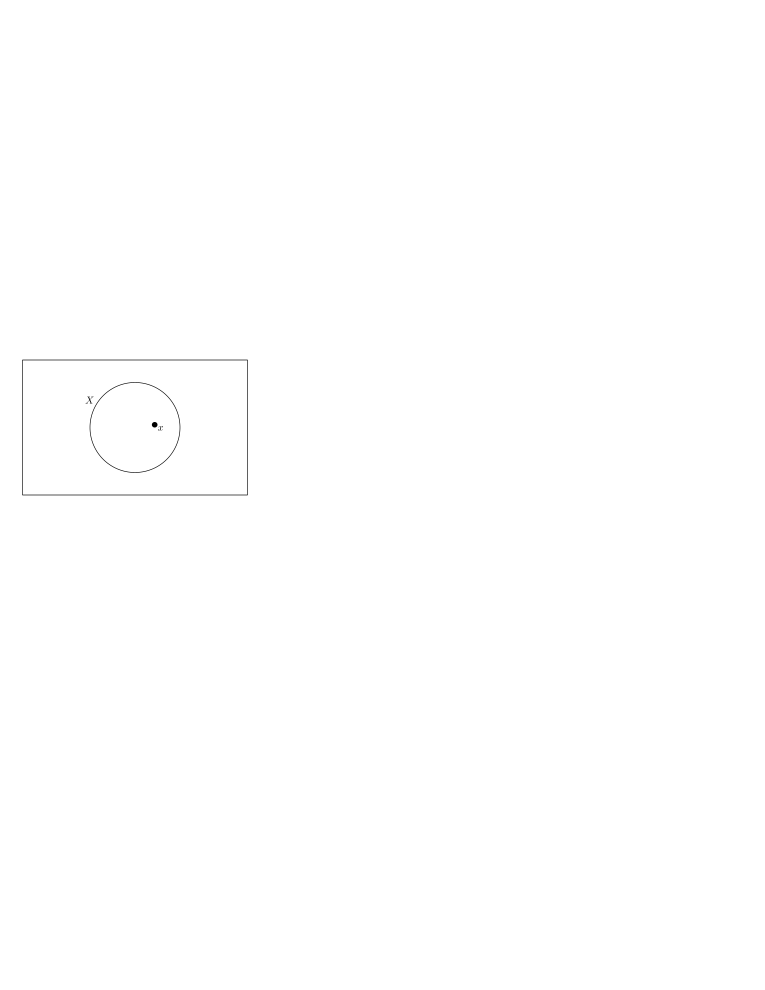
\includegraphics{../graphics/set1.pdf}
\]

\begin{definition} 
A \textbf{subset}\index{subset} $Y$ of a set $X$ is a set $Y$ such
that every element of $Y$ is also an element of $X$. We denote this
by:
\[
Y\subset X\index{set theory symbols!subset@$\subset$}
\] 
\end{definition}

If $Y$ is contained in $X$, we will sometimes loosely say that $X$ is
\textit{bigger} than $Y$.

\begin{question} 
Can you think of a set $X$ and a subset $Y$ where saying $X$ is bigger
than $Y$ is a bit misleading?
\end{question}
\QM

\begin{question} 
How is the meaning of the symbol $\in$ different from the meaning of
the symbol $\subset$?
\end{question}
\QM


\subsection{Union}


\begin{definition}\index{union}\index{u@$\cup$}\index{set theory symbols!union@$\cup$} Given two sets $X$ and $Y$, $X$ \textbf{union} $Y$ is the set of all the elements in $X$ or $Y$. We denote this by $X\cup Y$.
\end{definition}

Pictorially, we can imagine this as:

\[
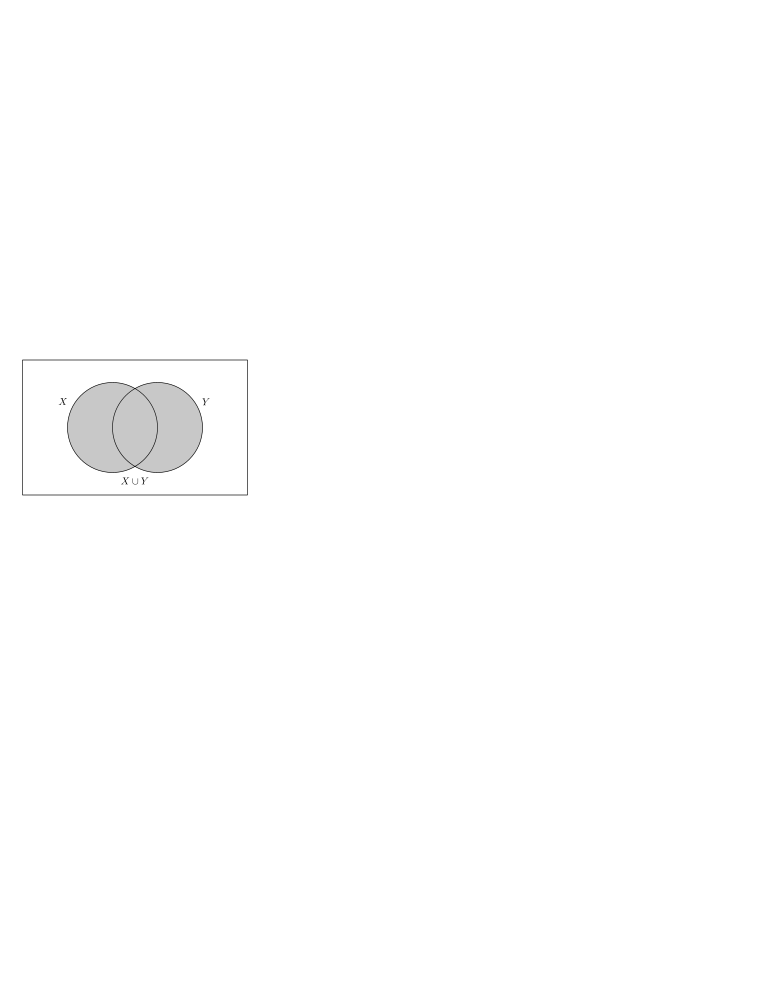
\includegraphics{../graphics/set2.pdf}
\]



\subsection{Intersection}

\begin{definition}\index{intersection}\index{set theory symbols!intersection@$\cap$} Given two sets $X$ and $Y$, 
$X$ \textbf{intersect} $Y$ is the set of all the elements that are simultaneously in $X$ and in $Y$. We denote this by $X\cap Y$. 
\end{definition}

Pictorially, we can imagine this as:
\[
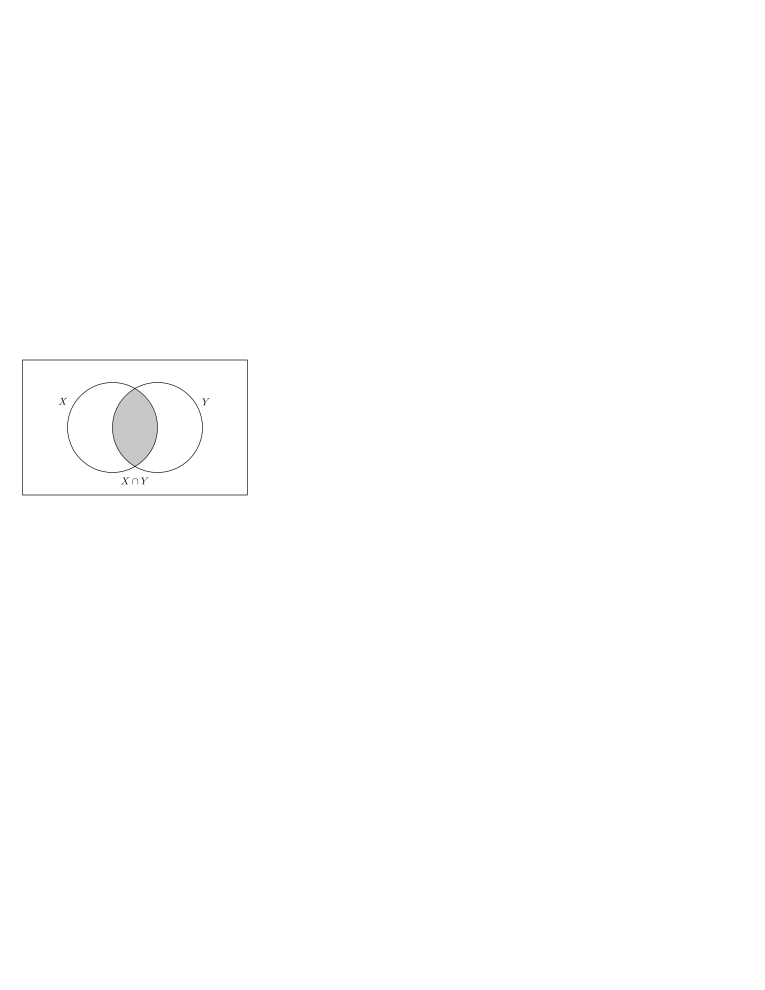
\includegraphics{../graphics/set3.pdf}
\]

\begin{question} Consider the sets $X$ and $Y$ below:
\[
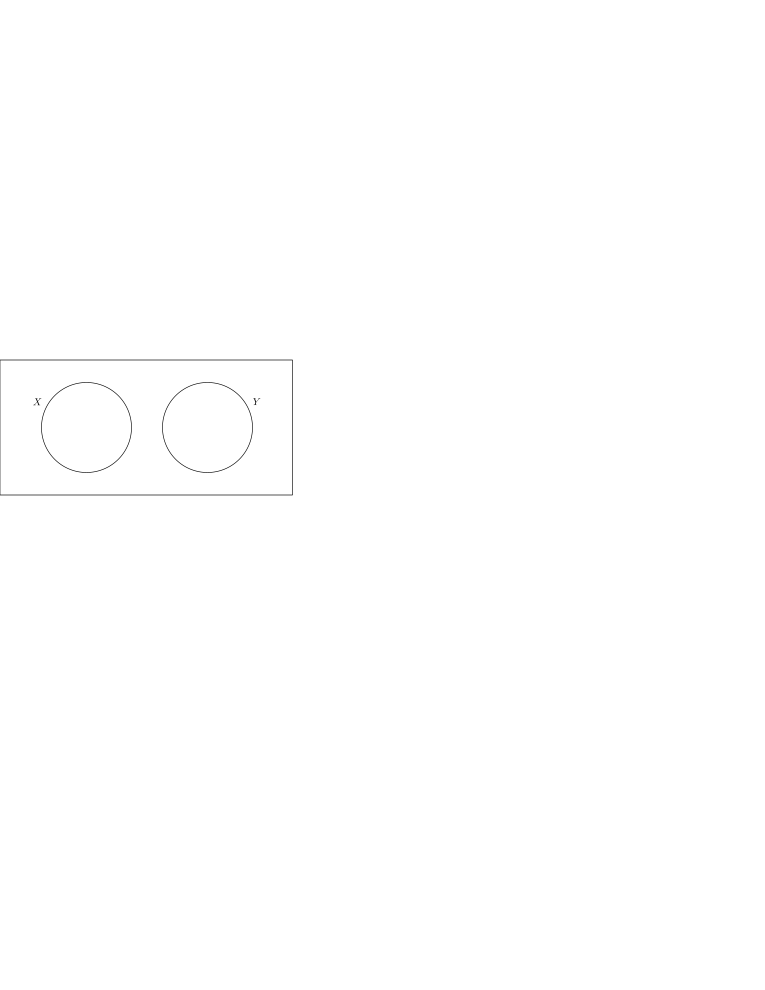
\includegraphics{../graphics/set4.pdf}
\]
What is $X\cap Y$?
\end{question}

I'll take this one: Nothing! We have a special notation for the set with no elements, it is called the \index{empty set}\textbf{empty set}. We denote the empty set by the symbol $\emptyset$.\index{set theory symbols!emptyset@$\emptyset$}




\subsection{Complement}

\begin{definition}\index{complement}\index{set theory symbols!complement@$-$} Given two sets $X$ and $Y$, 
$X$ \textbf{complement} $Y$ is the set of all the elements that are in $X$ and are not in $Y$. We denote this by $X-Y$.
\end{definition}

Pictorially, we can imagine this as:
\[

\includegraphics{../graphics/set5.pdf}
\]

\begin{question} Check out the two sets below:
\[
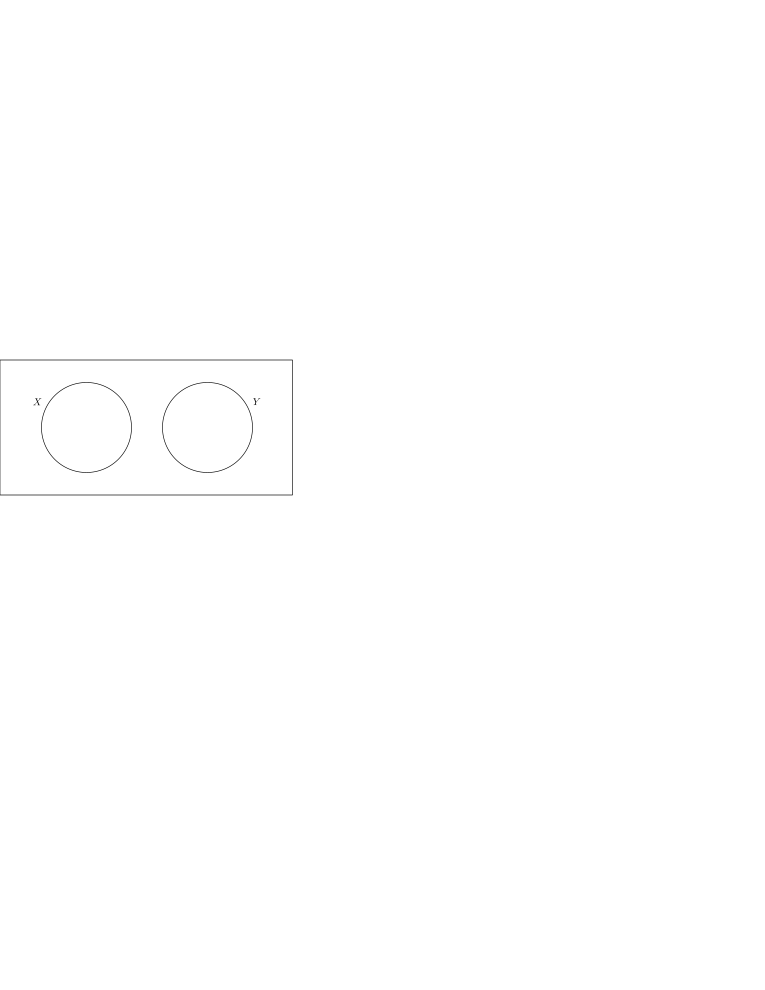
\includegraphics{../graphics/set4.pdf}
\]
What is $X-Y$? What is $Y-X$?
\end{question}
\QM


\subsection{Putting Things Together}

OK, let's try something more complex:

\begin{question} Prove that:
\[
X\cup (Y \cap Z) = (X \cup Y)\cap (X \cup Z)
\]
\end{question}

\begin{proof} 
Look at the left-hand side of the equation first. We can represent the
elements in $Y\cap Z$ with shaded region in the following diagram:
\[
\includegraphics{../graphics/setproof.pdf}
\]
So the union of this region with $X$ is represented the shaded
region in this diagram.
\[
\includegraphics{../graphics/setproof1.pdf}
\]
Now, looking at the right-hand side of the equation, $X\cup Y$ is
represented by this shaded region:
\[
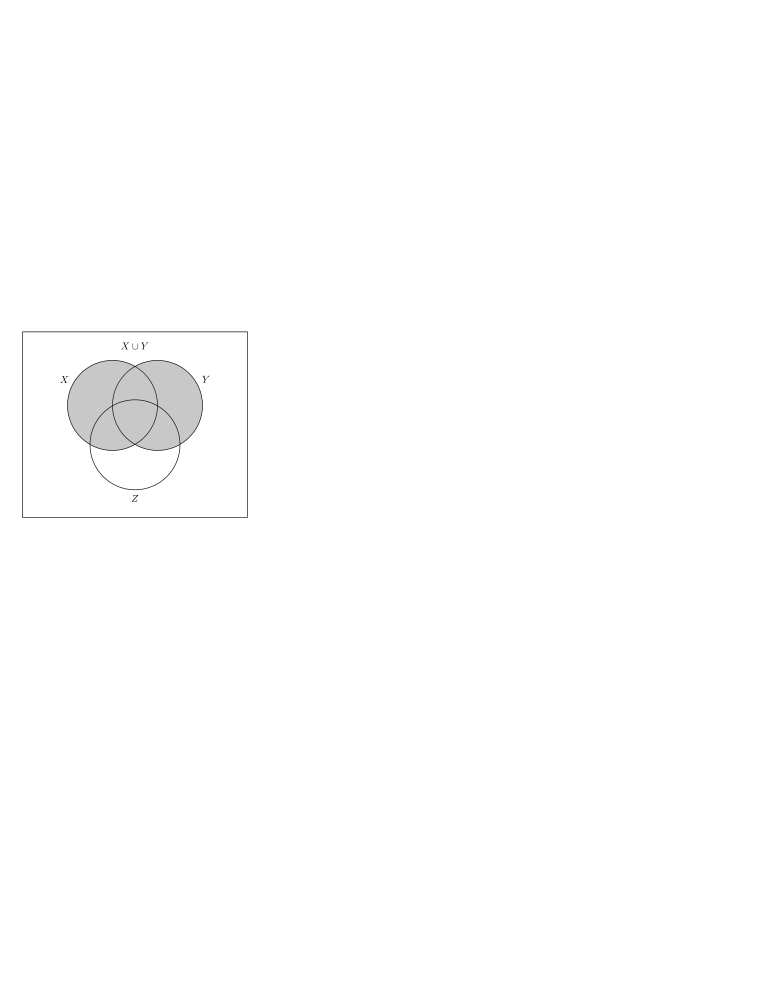
\includegraphics{../graphics/setproof2.pdf}
\]
And $X\cup Z$ is represented by this shaded region:
\[
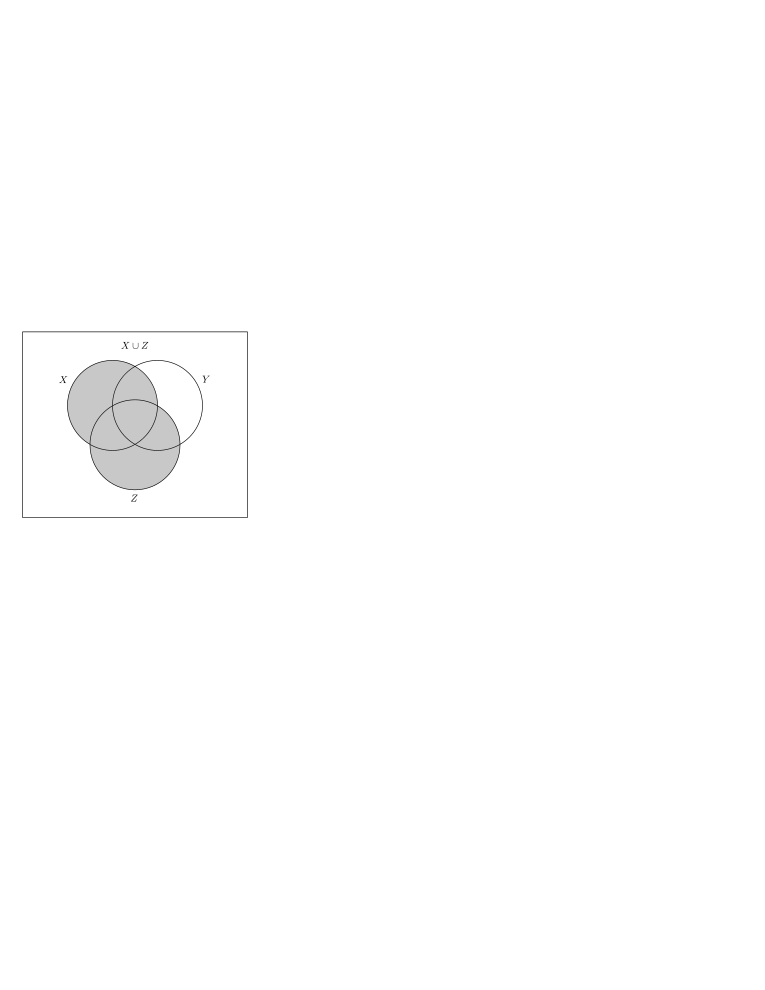
\includegraphics{../graphics/setproof3.pdf}
\]
The region shaded in both of the diagrams, which is the
intersection of $X\cup Y$ and $X\cup Z$, is represented by the shaded
region below.
\[
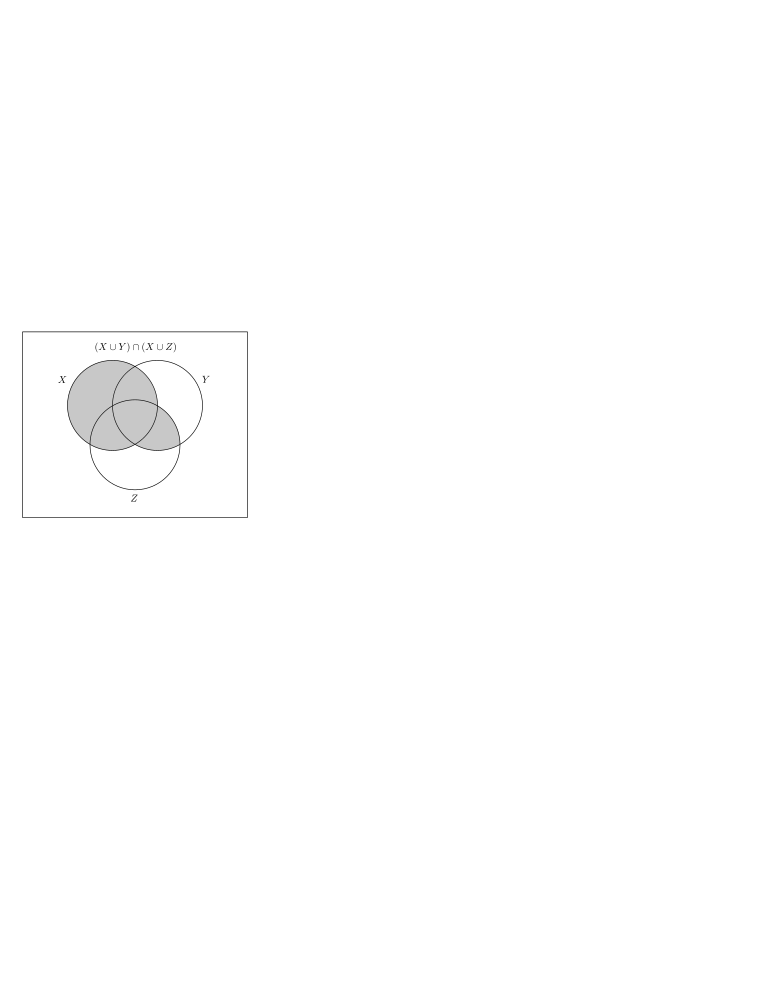
\includegraphics{../graphics/setproof4.pdf}
\]
Comparing the diagrams representing the left-hand and right-hand sides
of the equation, we see that the same regions are shaded, and so we
are done.
\end{proof}

\begin{problems}

\begin{enumerate}
\item Given two sets $X$ and $Y$, explain what is meant by $X\cup Y$.
\item Given two sets $X$ and $Y$, explain what is meant by $X\cap Y$.
\item Given two sets $X$ and $Y$, explain what is meant by $X - Y$.
\item Explain the difference between the symbols $\in$ and $\subset$.
\item If we let $X$ be the set of ``right triangles'' and we let $Y$ be the set of ``equilateral triangles'' does the picture below show the relationship between these two sets?
\[
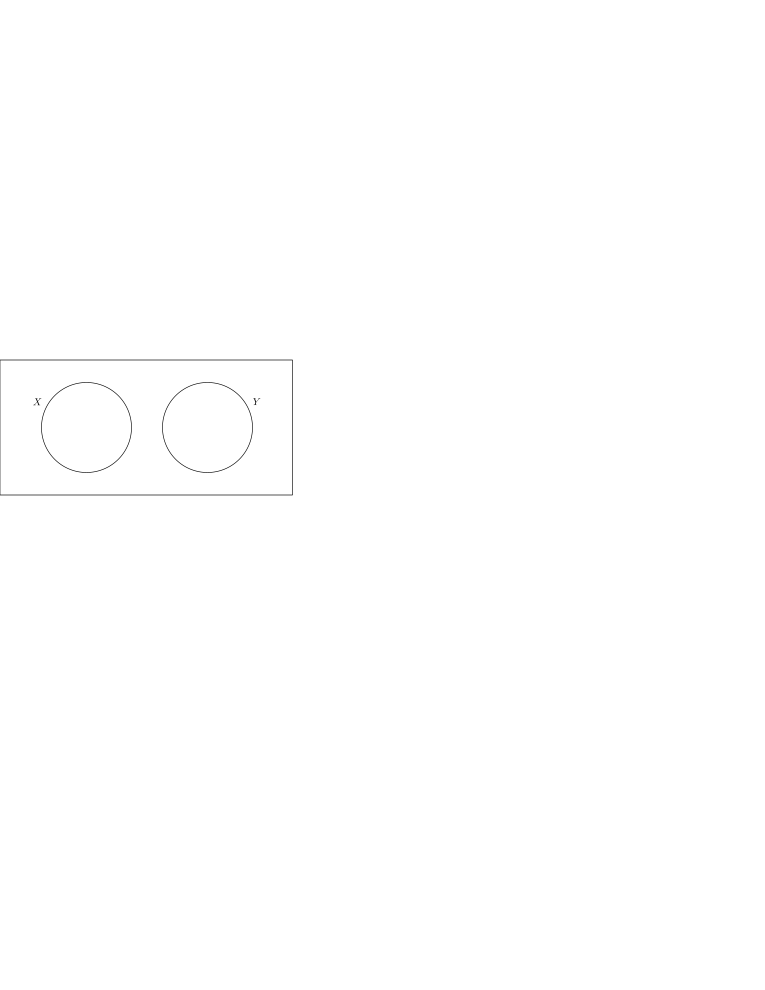
\includegraphics{../graphics/set4.pdf}
\]
Explain your reasoning.
\item If $X = \{1,2,3,4,5\}$ and $Y = \{3,4,5,6\}$ find:
\begin{enumerate}
\item $X\cup Y$
\item $X\cap Y$
\item $X-Y$
\item $Y-X$
\end{enumerate}
In each case explain your reasoning. 
\item Let $n\Z$ represent the integer multiples of $n$. So for example:
\[
3\Z = \{\dots,-12,-9,-6,-3,0,3,6,9,12,\dots\}
\]
Compute the following:
\begin{enumerate}
\item $3\Z\cap 4\Z$
\item $2\Z\cap 5\Z$
\item $3\Z\cap 6\Z$
\item $4\Z\cap 6\Z$
\item $4\Z\cap 10\Z$
\end{enumerate}
In each case explain your reasoning. 
\item Make a general rule for intersecting sets of the form $n\Z$ and
  $m\Z$. Explain why your rule works.
\item Prove that:
\[
X = (X\cap Y) \cup (X-Y)
\]
\item Prove that:
\[
X-(X-Y) = (X\cap Y)
\]
\item Prove that:
\[
X \cup (Y-X) = (X\cup Y)
\]
\item Prove that:
\[
X \cap (Y-X) = \emptyset
\]
\item Prove that:
\[
(X-Y)\cup (Y-X) = (X\cup Y)-(X\cap Y)
\]
\item Prove that:
\[
X\cup (Y \cap Z) = (X \cup Y)\cap (X \cup Z)
\]
\item Prove that:
\[
X\cap (Y \cup Z) = (X \cap Y)\cup (X \cap Z)
\]
\item Prove that:
\[
X - (Y \cap Z) = (X -Y)\cup (X - Z)
\]
\item Prove that:
\[
X - (Y \cup Z) = (X -Y)\cap (X -Z)
\]
\item If $X\cup Y = X$, what can we say about the relationship between the sets $X$ and $Y$? Explain your reasoning.
\item If $X\cup Y = Y$, what can we say about the relationship between the sets $X$ and $Y$? Explain your reasoning.
\item If $X\cap Y = X$, what can we say about the relationship between the sets $X$ and $Y$? Explain your reasoning.
\item If $X\cap Y = Y$, what can we say about the relationship between the sets $X$ and $Y$? Explain your reasoning.
\item If $X-Y =\emptyset$, what can we say about the relationship between the sets $X$ and $Y$? Explain your reasoning.
\item If $Y-X =\emptyset$, what can we say about the relationship between the sets $X$ and $Y$? Explain your reasoning.
\end{enumerate}
\end{problems}


\newpage



\section{Tessellations}

Go to the internet and look up M.C.\ Escher.\index{Escher, M.C.} He
was an artist. Look at some of his work. When you do your search be
sure to include the word ``tessellation'' OK? Back already? Very
good. Sometimes Escher worked with tessellations. What's a
tessellation? I'm glad you asked:

\begin{definition}\index{tessellation} A \textbf{tessellation} is a pattern of 
polygons fitted together to cover the entire plane without
overlapping.  
\end{definition}
While it is impossible to actually cover the entire plane with shapes,
if we give you enough of a tessellation, you should be able to continue
it's pattern indefinitely.  Here are pieces of tessellations:
\[
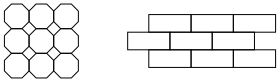
\includegraphics{../graphics/semiRegTess.pdf}
\]
On the left we have a tessellation of a square and an octagon. On the
right we have a ``brick-like'' tessellation.

\begin{definition}\index{tessellation!regular}\index{regular!tessellation}
A tessellation is called a \textbf{regular tessellation} if it is
composed of copies of a single regular polygon and these polygons meet
vertex to vertex.\index{regular!polygon}
\end{definition}


\begin{example} Here are some examples of regular tessellations:
\[
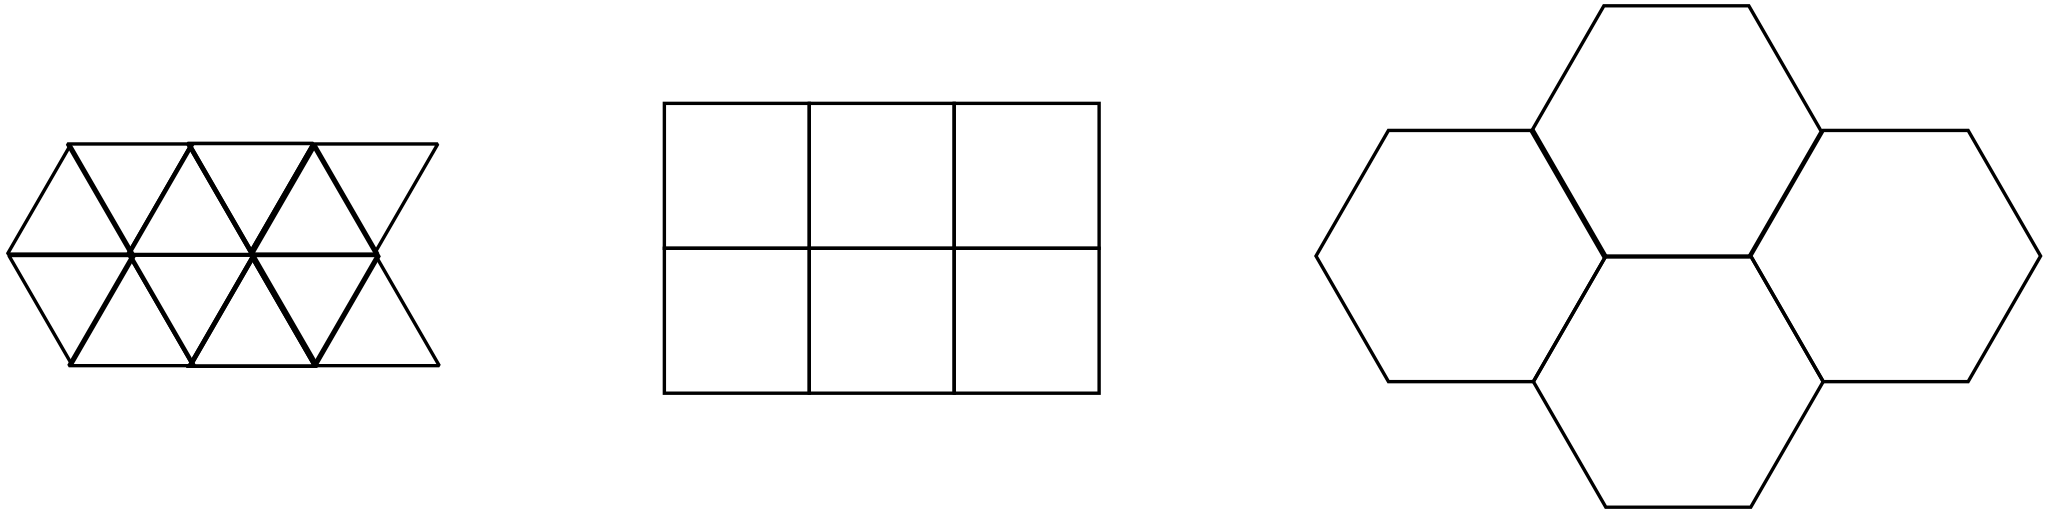
\includegraphics{../graphics/regtess.pdf}
\]
\end{example}

Johannes Kepler\index{Kepler, Johannes}, who lived from 1571--1630,
was one of the first people to study tessellations. He certainly knew
the next theorem:

\begin{theorem} There are only $3$ regular tessellations.
\end{theorem}

\begin{question} Why is the theorem above true?
\end{question}
\QM

Since one can prove that there are only three regular tessellations,
and we have shown three above, then that is all of them. On the other
hand there are lots of nonregular tessellations. Here are two
different ways to tessellate the plane with a
triangle:\index{tessellation!triangles}
\[
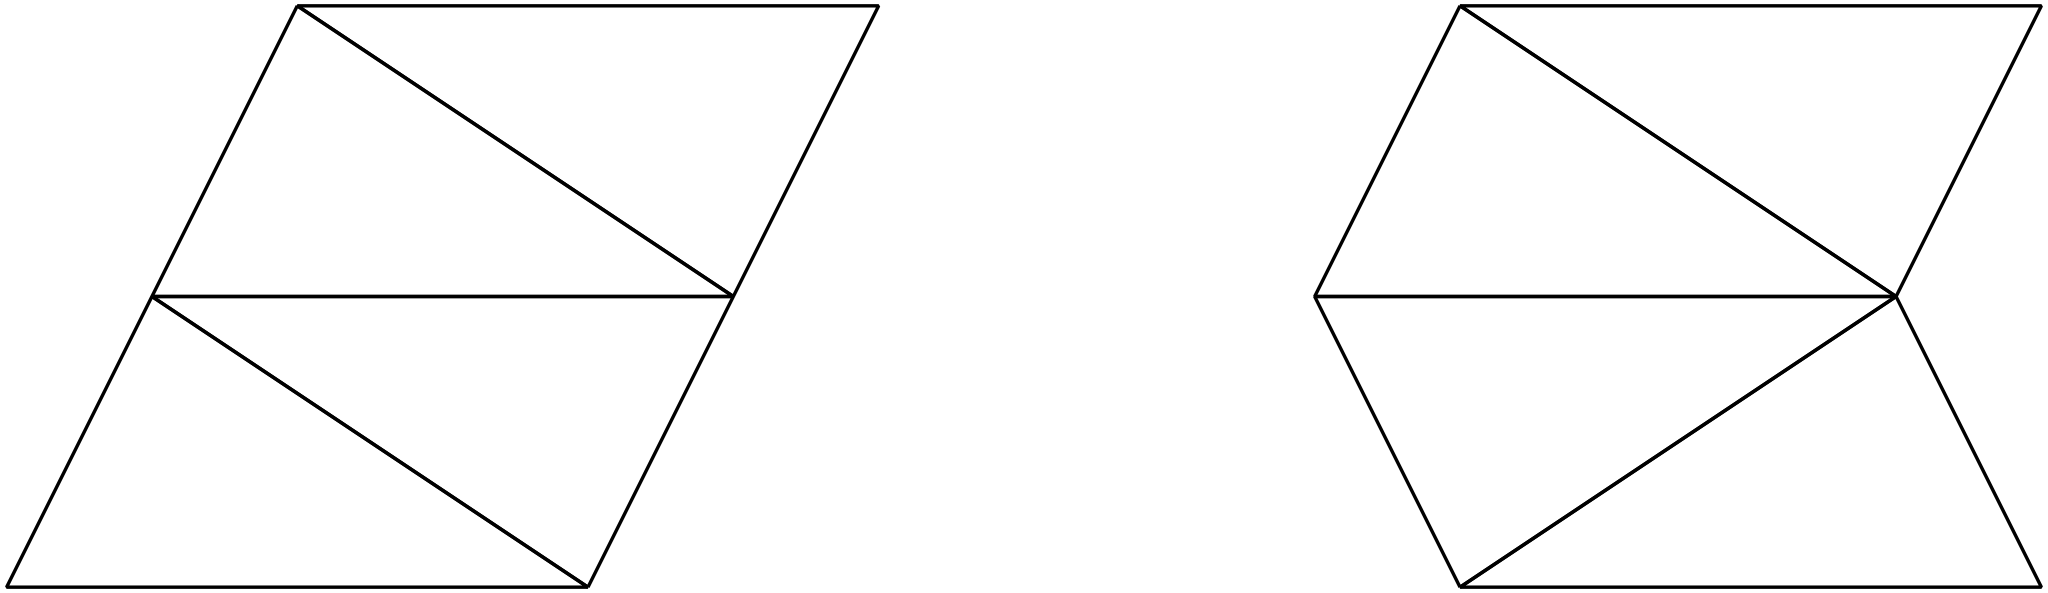
\includegraphics{../graphics/triangletess.pdf}
\]
Here is a way that you can tessellate the plane with any old
quadrilateral:
\[\index{tessellation!any quadrilateral}\index{quadrilateral!tessellation of}
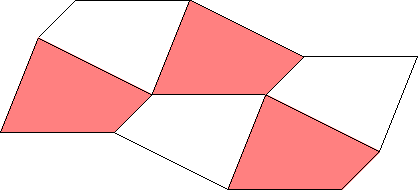
\includegraphics{../graphics/quadtess.pdf}
\]

\subsection{Tessellations and Art}

How does one make art with tessellations? To start, a little
decoration goes a long way. Check this out: Decorate two squares as
such:
\[
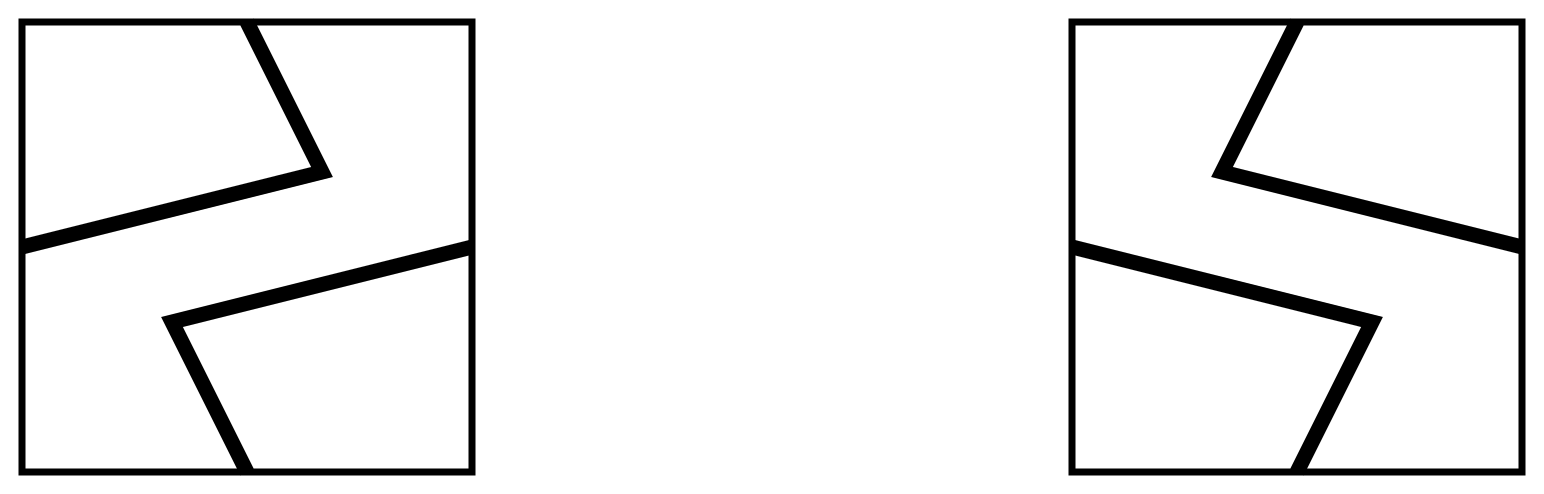
\includegraphics{../graphics/lightningsquares.pdf}
\]
Tessellate them randomly in the plane to get this lightning-like picture:
\[

\includegraphics{../graphics/lightningtess.pdf}
\]
\begin{question} 
What sort of picture do you get if you tessellate these decorated
squares randomly in a plane?
\[
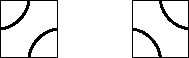
\includegraphics{../graphics/watersquares.pdf}
\]
\end{question}
\QM

Another way to go is to start with your favorite tessellation:
\[
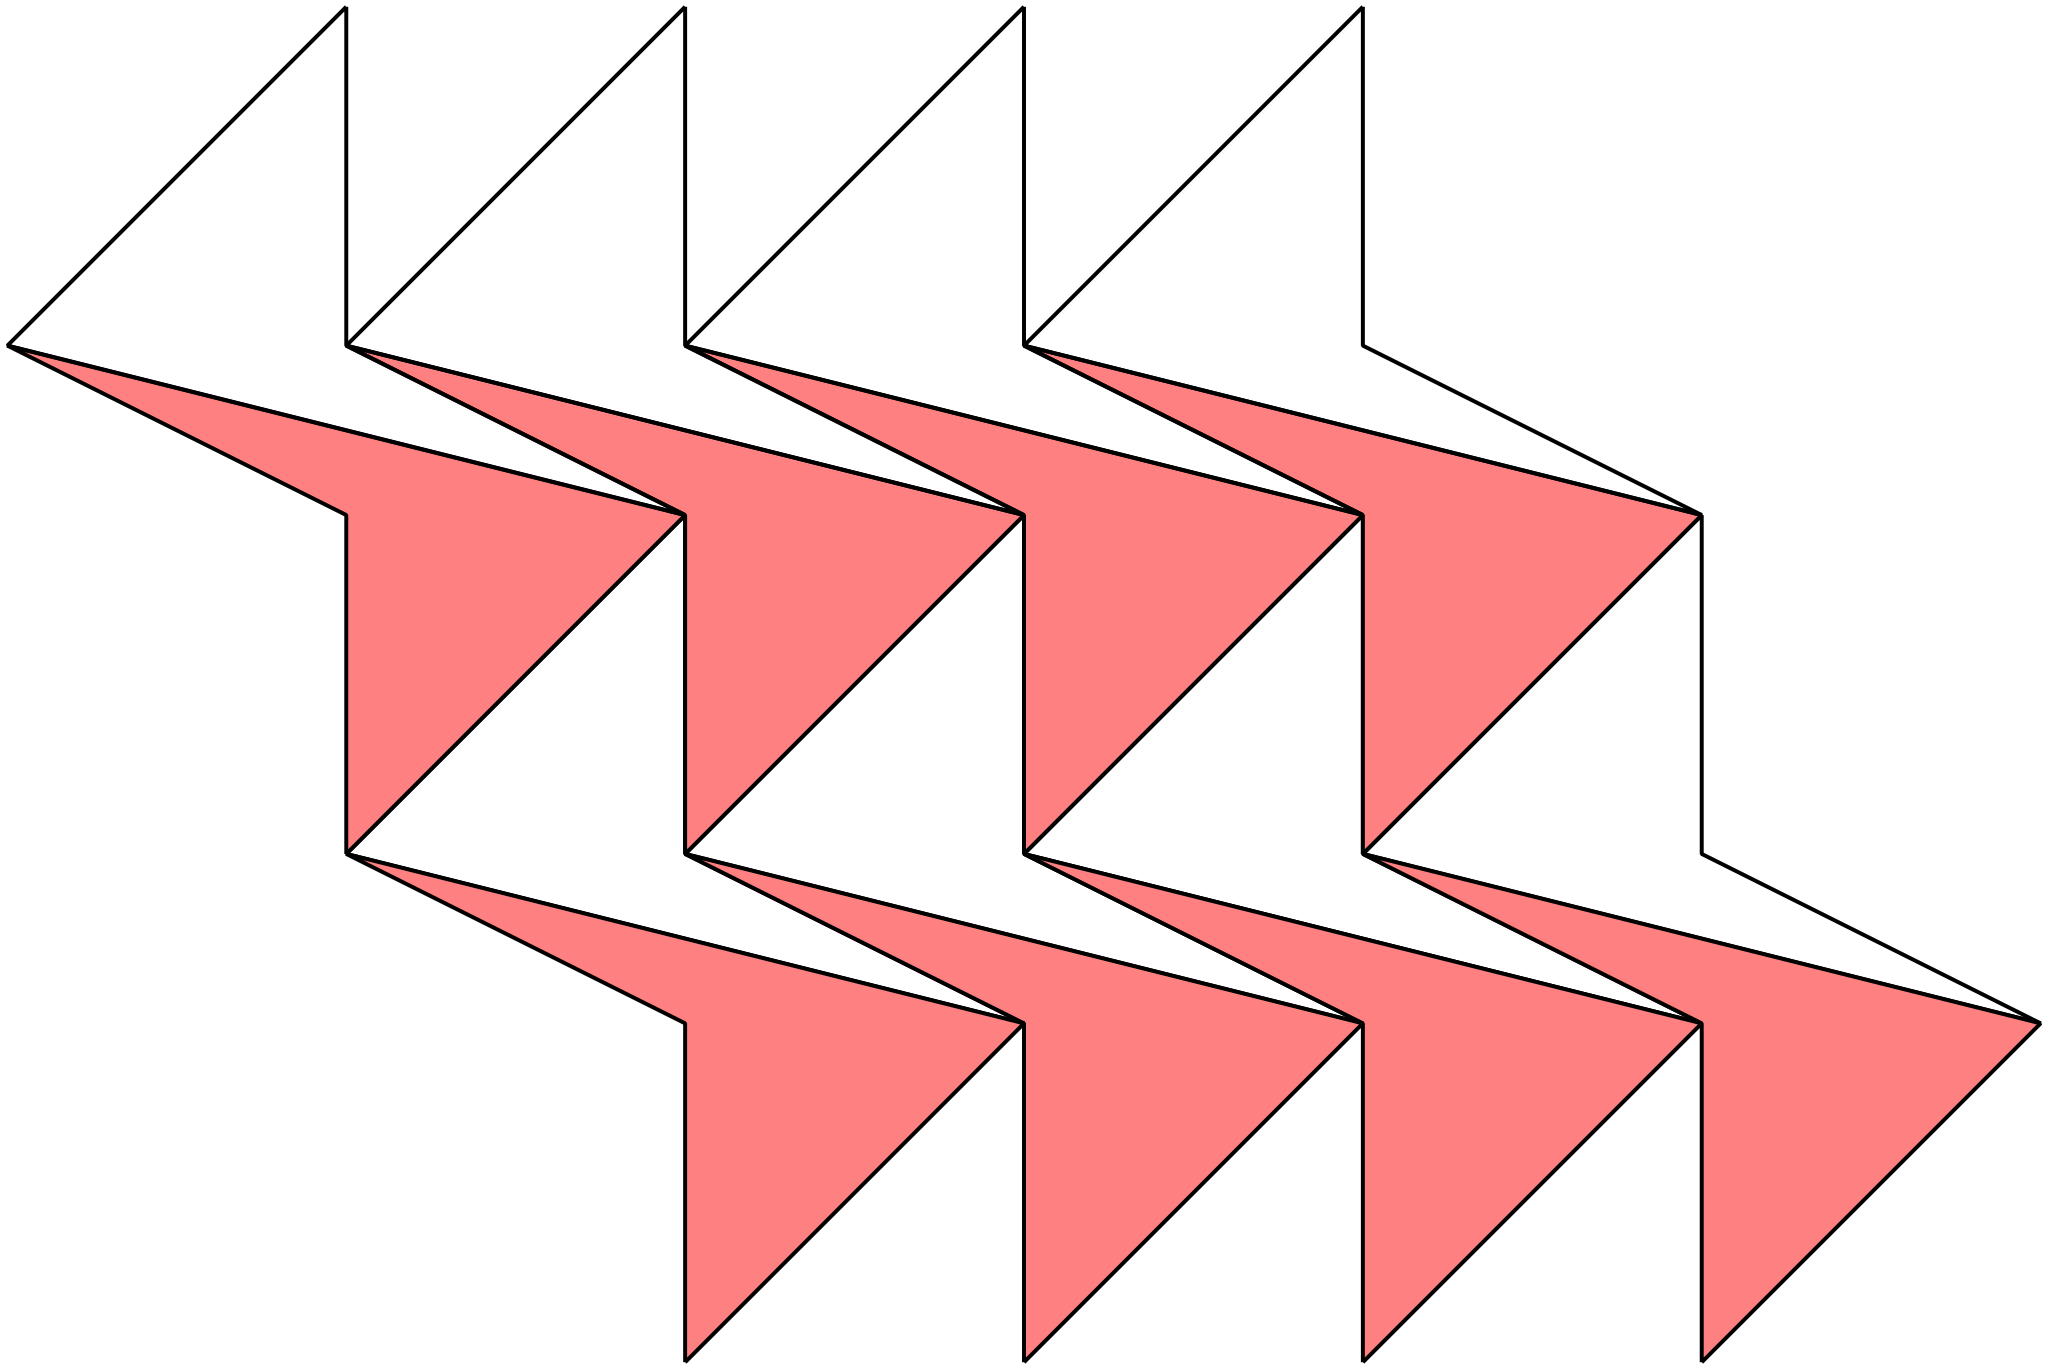
\includegraphics{../graphics/nonconvextess.pdf}
\]
Then you modify it a bunch to get something different:
\[
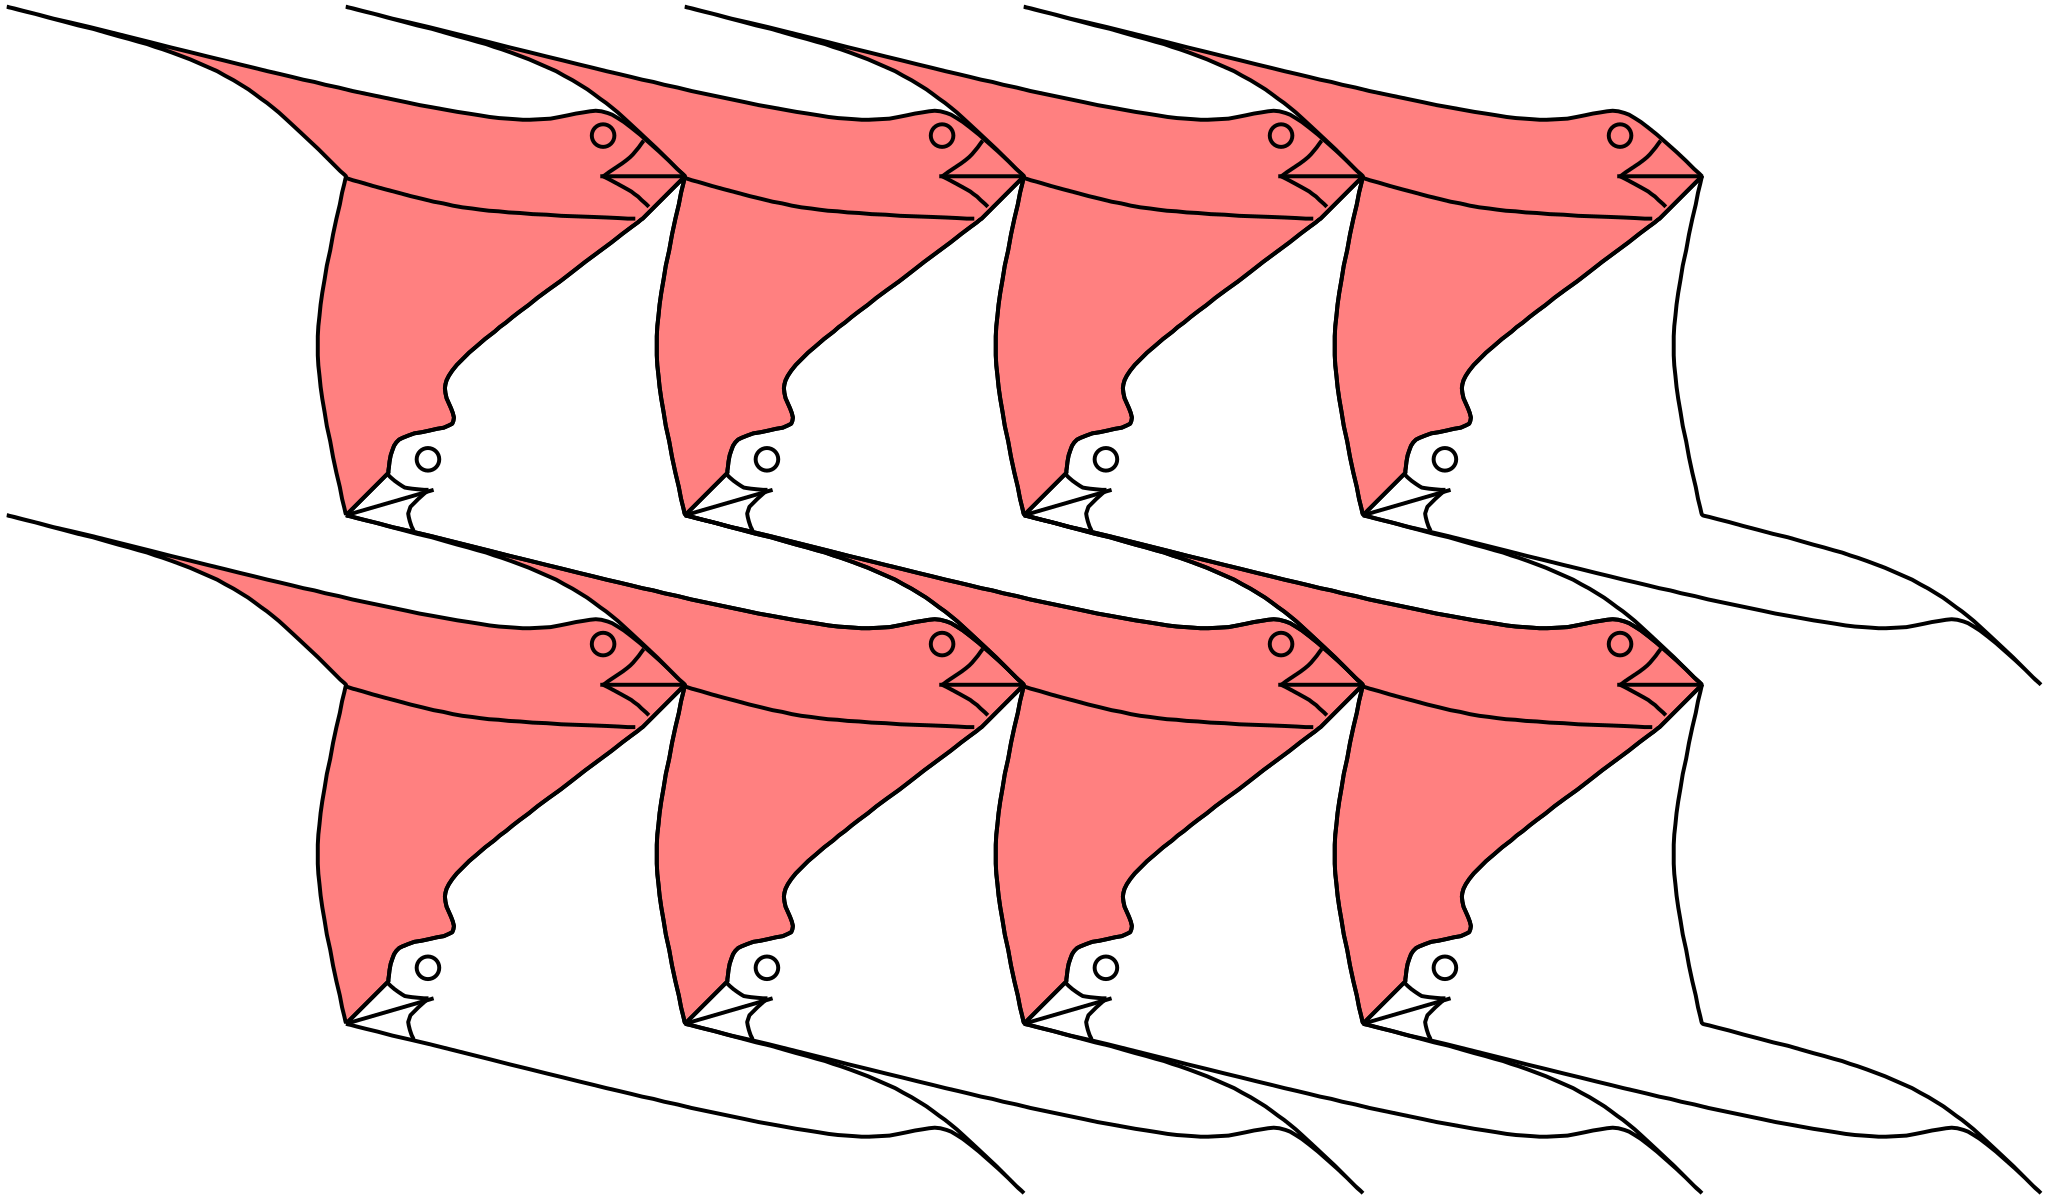
\includegraphics{../graphics/birdstess.pdf}
\]

\begin{question} What kind of art can you make with tessellations?
\end{question}
\QM


I'm not a very good artist, but I am a mathematician. So let's use a
tessellation to give a proof! Let me ask you something:

\begin{question} What is the most famous theorem in mathematics? 
\end{question}
Probably the Pythagorean Theorem comes to mind. Let's recall the statement of the Pythagorean Theorem:

\begin{theorem}[Pythagorean Theorem]\index{Pythagorean Theorem} Given a right triangle, the sum of the squares of the 
lengths of the two legs equals the square of the length of 
the hypotenuse.  Symbolically, if $a$ and $b$ represent the 
lengths of the legs and $c$ is the length of the hypotenuse, 
\[
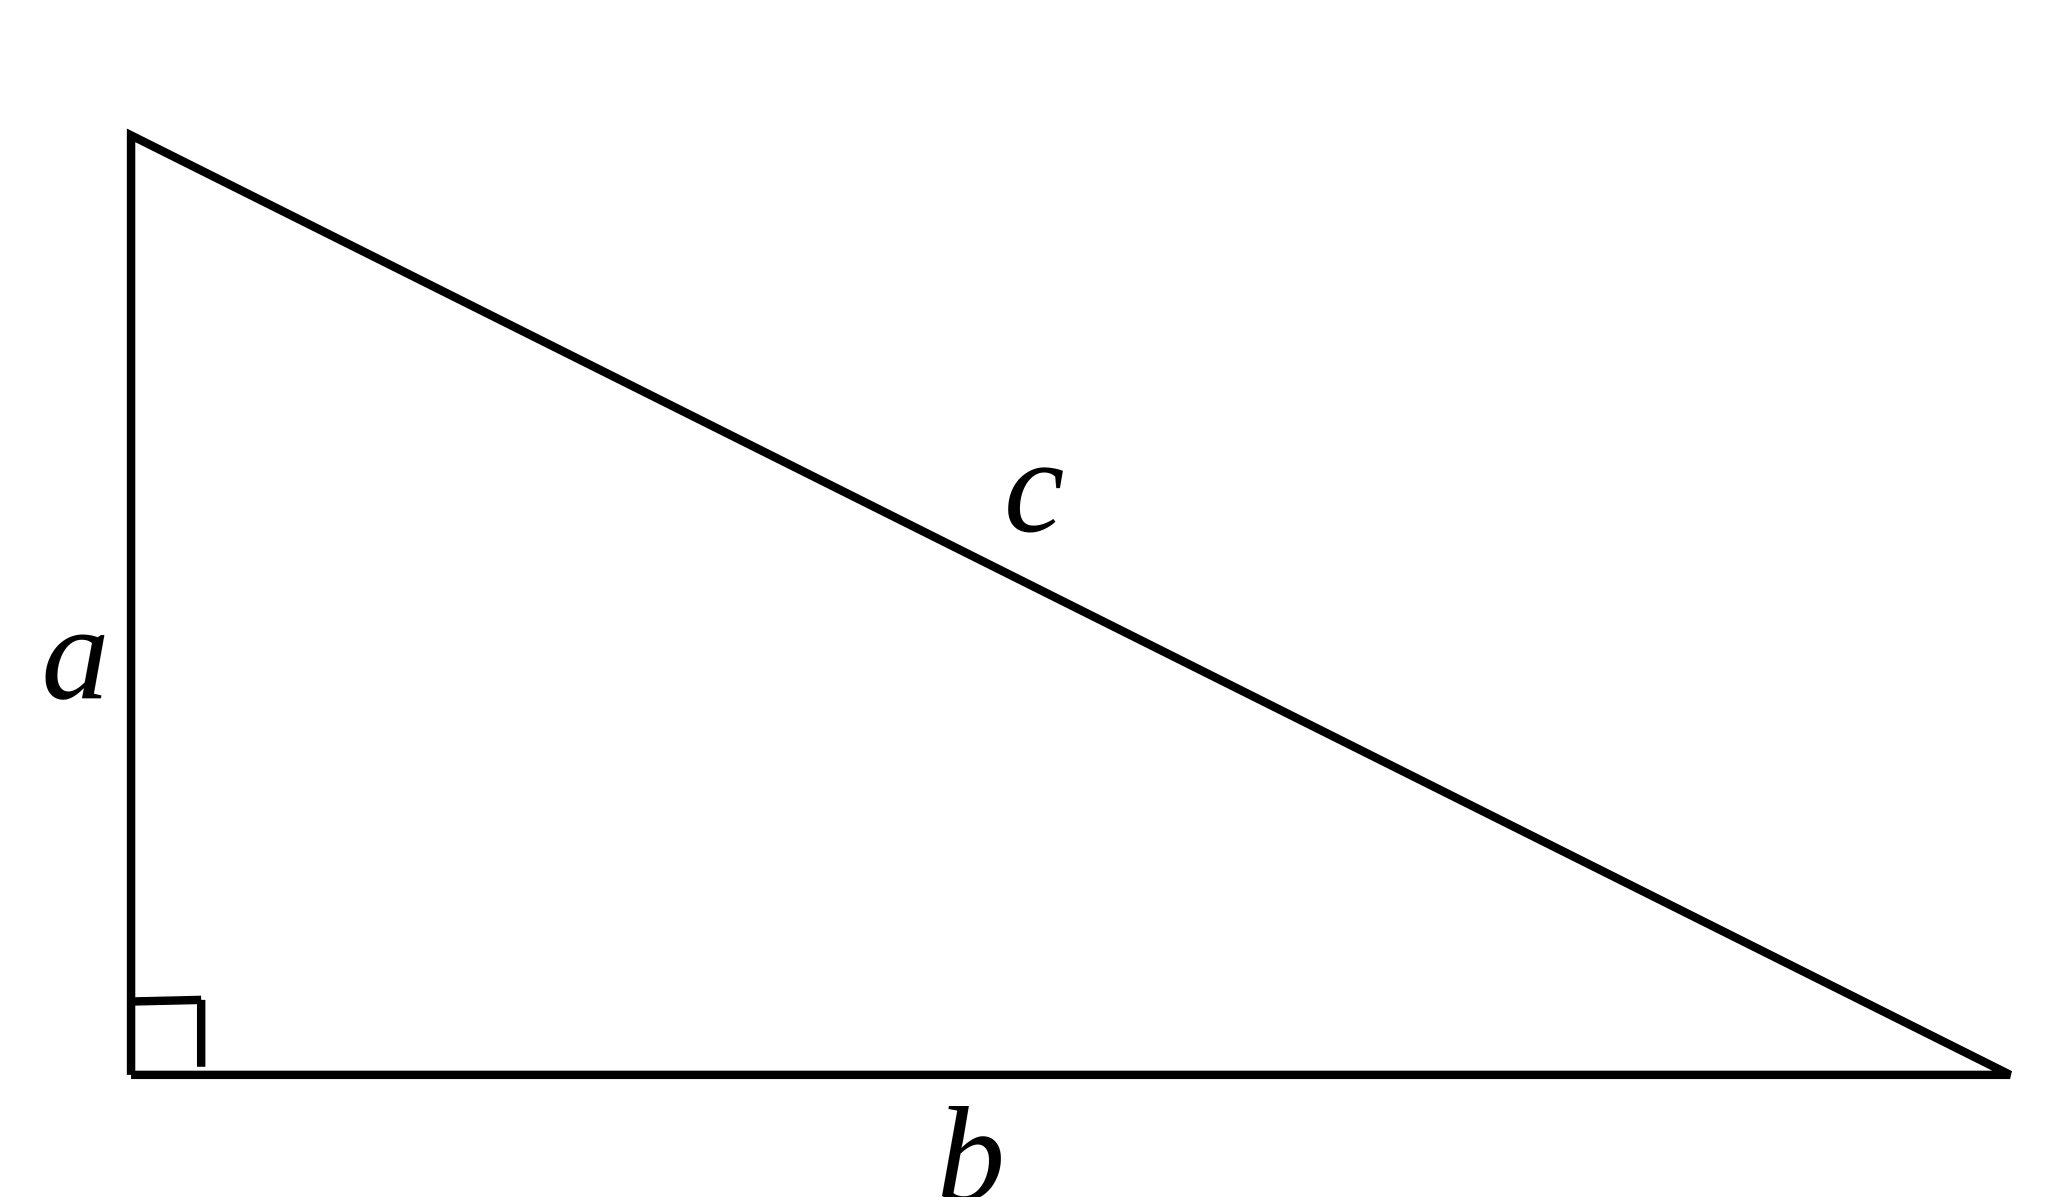
\includegraphics{../graphics/pbppyth.pdf}
\]
then 
\[
a^2 + b^2 = c^2.
\]
\end{theorem}


Let's give a proof! Check out this tessellation involving $2$ squares:
\[
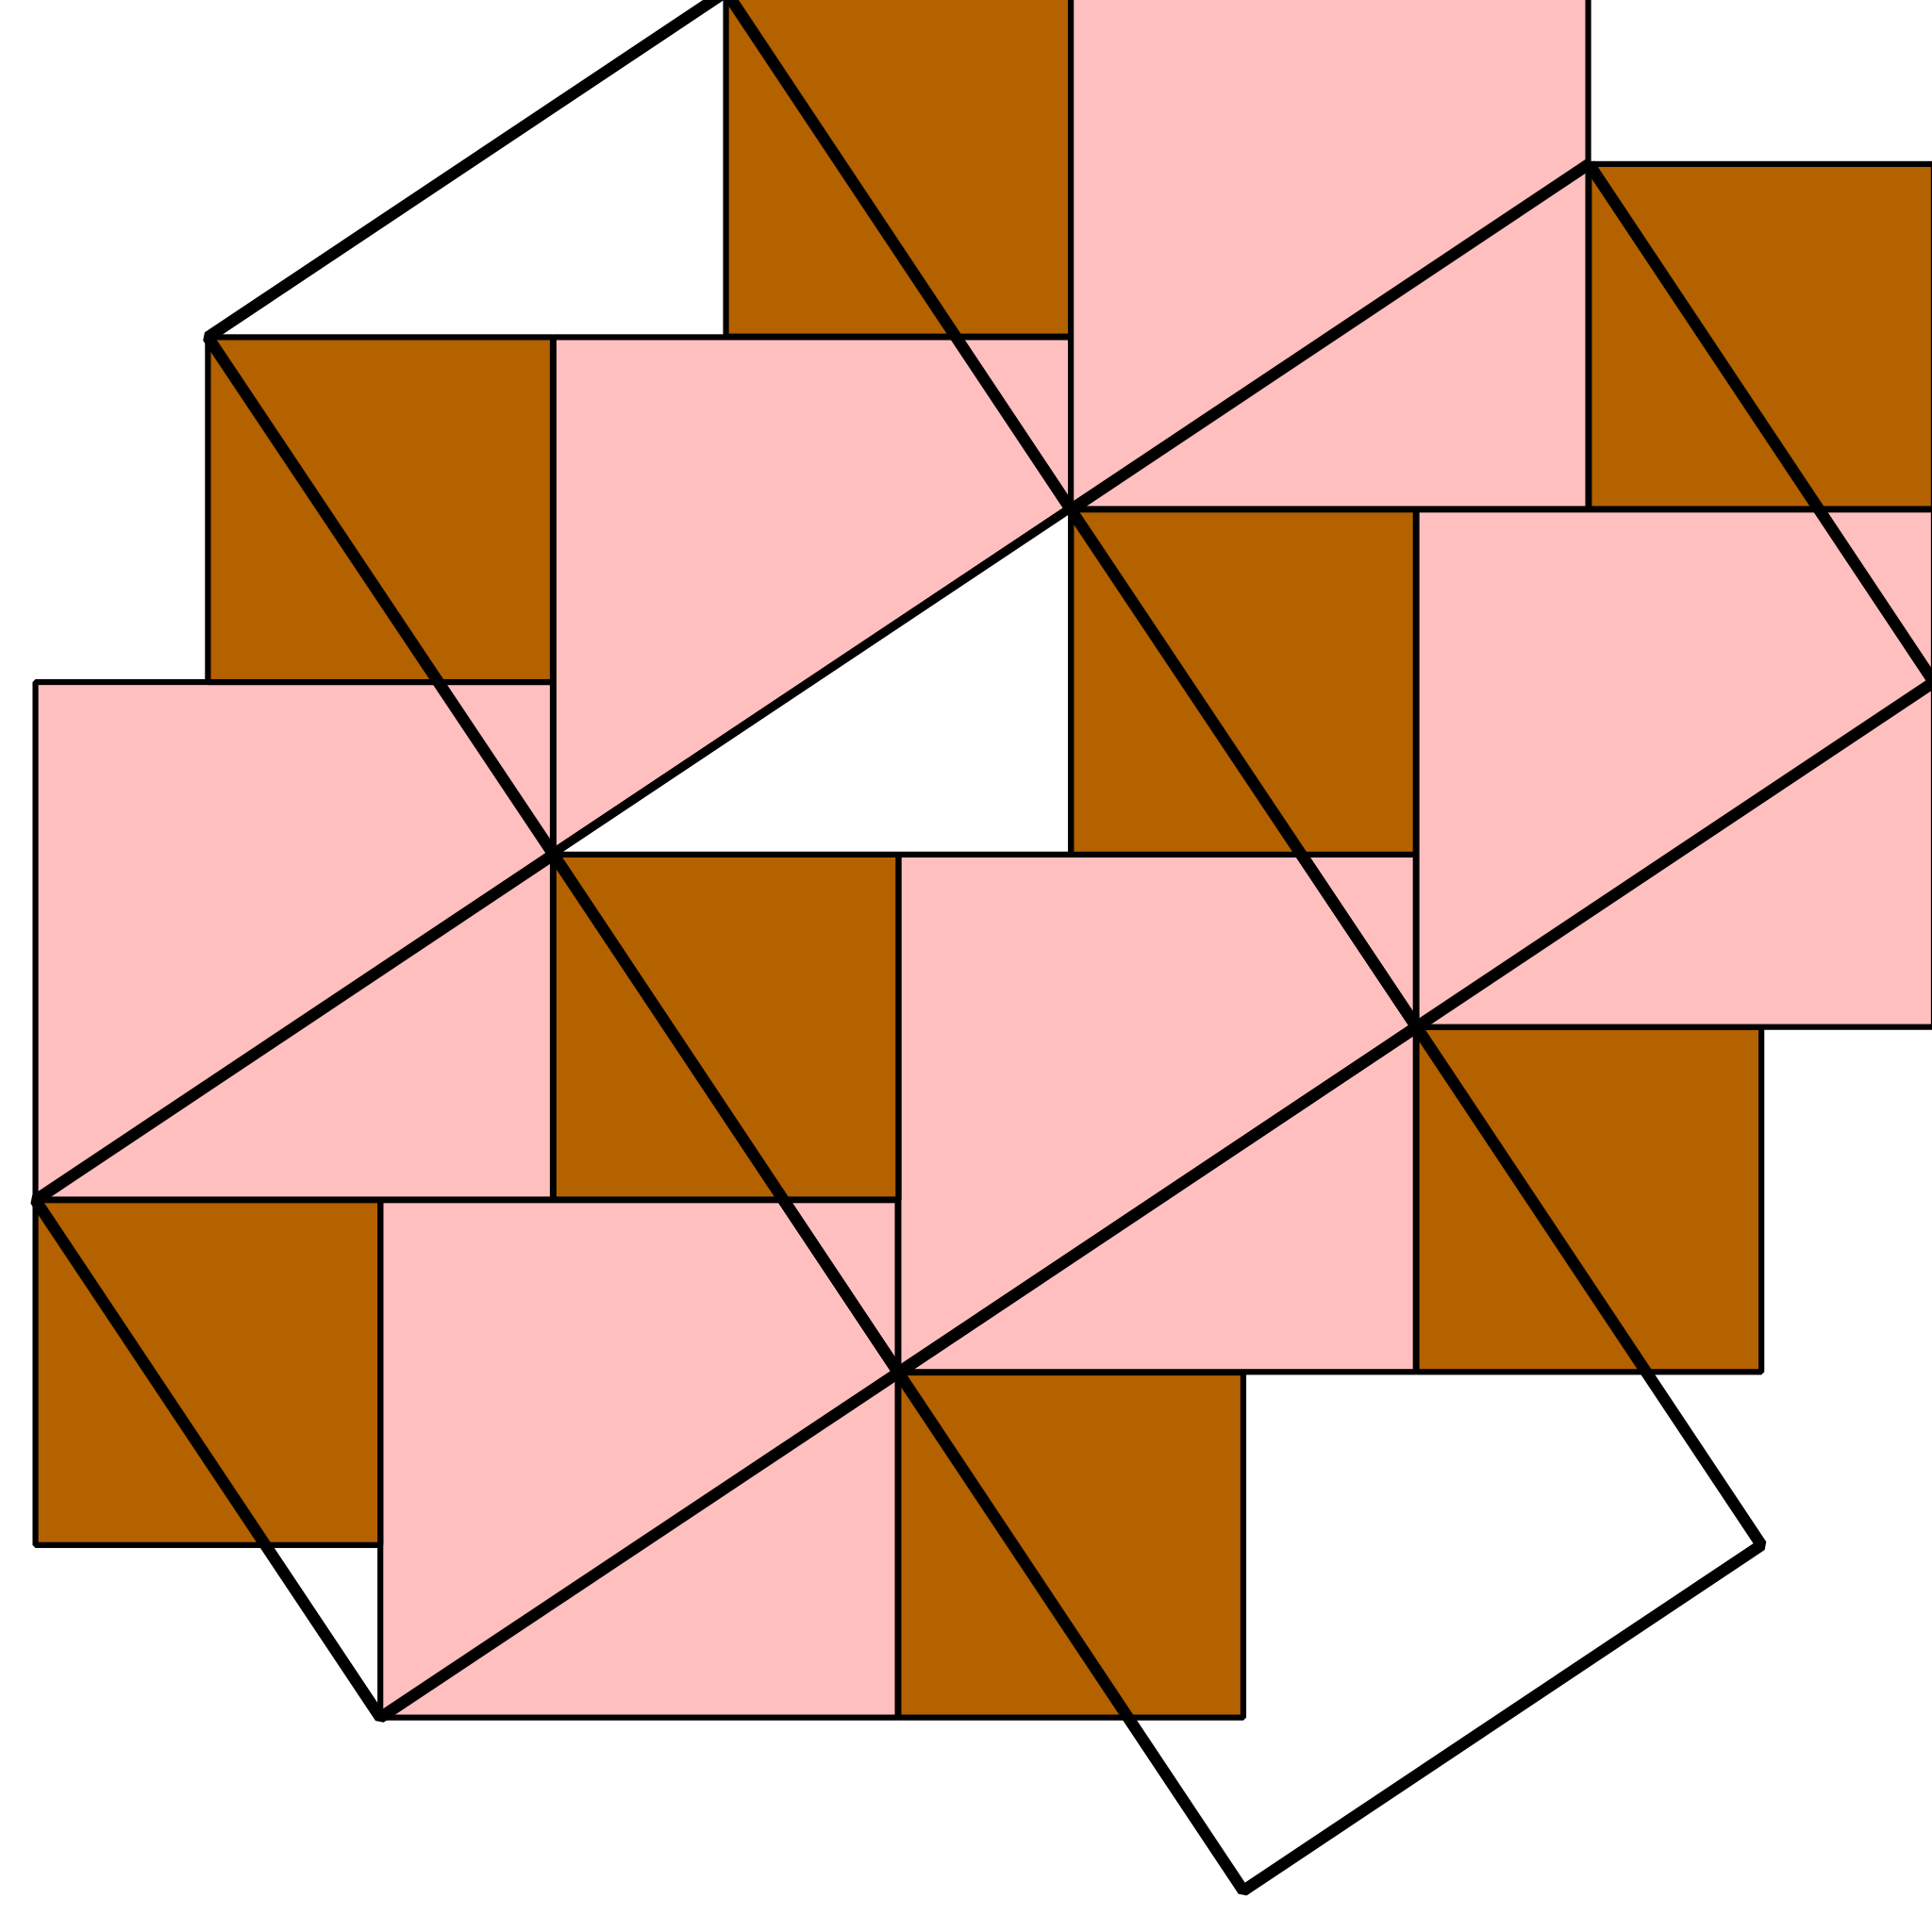
\includegraphics{../graphics/pbppyth2.pdf}
\]
\begin{question} How does the picture above ``prove'' the Pythagorean Theorem?
\end{question}
\begin{proof}[Solution]  
The white triangle is our right triangle. The area of the middle
overlaid square is $c^2$, the area of the small dark squares is $a^2$,
and the area of the medium lighter square is $b^2$. Now label all the
``parts'' of the large overlaid square:
\[
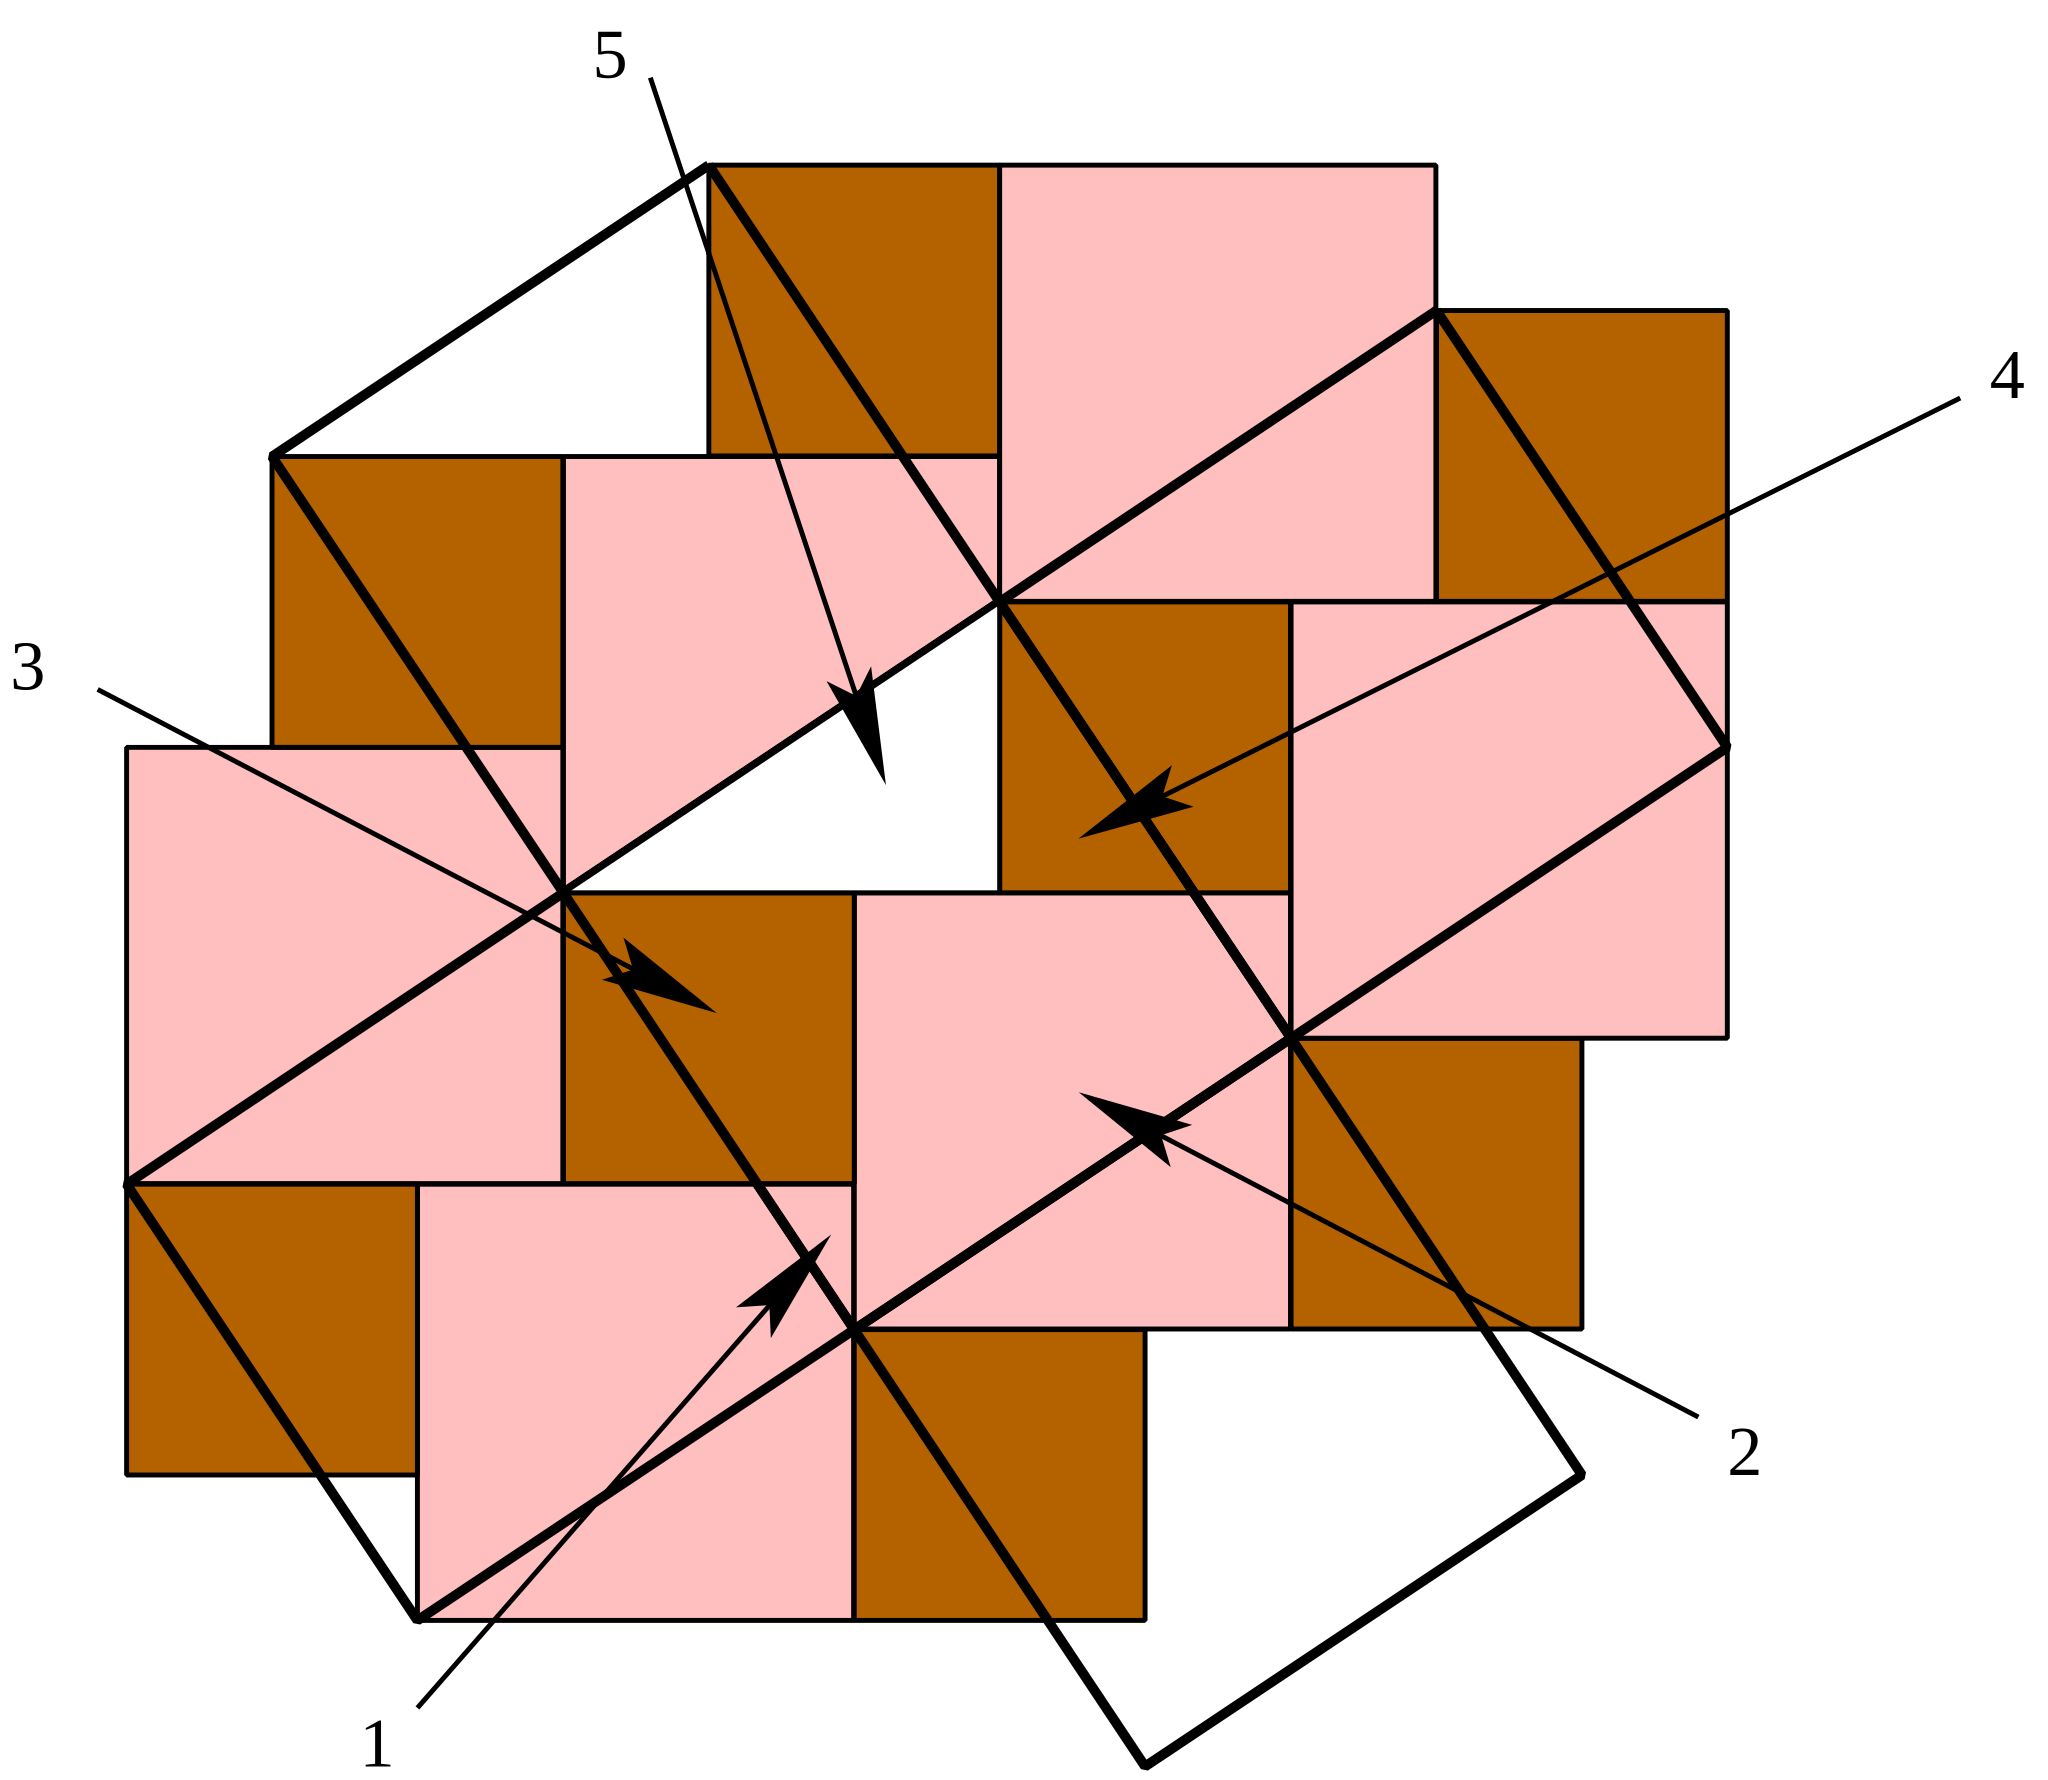
\includegraphics{../graphics/pbppyth2a.pdf}
\]
From the picture we see that
\begin{align*}
a^2 &= \{\text{3 and 4}\}\\
b^2 &= \{\text{1, 2, and 5}\}\\
c^2 &= \{\text{1, 2, 3, 4, and 5}\}
\end{align*}
Hence
\[
c^2 = a^2 + b^2
\]
Since we can always put two squares together in this pattern, this
proof will work for any right triangle.
\end{proof}

\begin{question} Can you use the above tessellation to give a dissection proof of the Pythagorean Theorem?
\end{question}
\QM



\begin{problems}

\begin{enumerate}
\item Show two different ways of tessellating the plane with a given scalene triangle. Label your picture as necessary.
\item Show how to tessellate the plane with a given quadrilateral. Label your picture.
\item Show how to tessellate the plane with a nonregular hexagon. Label your picture.
\item Give an example of a polygon with $9$ sides that tessellates the plane.
\item Give examples of polygons that tessellate and polygons that do
  not tessellate.
\item Give an example of a triangle that tessellates the plane where
  both $4$ and $8$ angles fit around each vertex.
\item True or False: Explain your conclusions.
\begin{enumerate}
\item There are exactly 5 regular tessellations.
\item Any quadrilateral tessellates the plane.
\item Any triangle will tessellate the plane.
\item If a triangle is used to tessellate the plane, then it is always
  the case that exactly $6$ angles will fit around each vertex.
\item If a polygon has more than 6 sides, then it cannot tessellate the plane.
\end{enumerate}
\item Given a regular tessellation, what is the sum of the angles
  around a given vertex?
\item Given that the regular octagon has $135$ degree angles, explain
  why you cannot give a regular tessellation of the plane with a
  regular octagon.
\item \label{tesstable} Fill in the following table:
\begin{center}
\begin{tabular}{|c || c| c| c|}\hline
 Regular & Does it      &  Measure & If it tessellates, how  \\
 $n$-gon & tessellate?  &  of an angle &  many surround each vertex?  \\
\hline\hline
$3$-gon &  &  &  \\ \hline
$4$-gon &  &  &  \\ \hline
$5$-gon &  &  &  \\ \hline
$6$-gon &  &  &  \\ \hline
$7$-gon &  &  &  \\ \hline
$8$-gon &  &  &  \\ \hline
$9$-gon &  &  &  \\ \hline
$10$-gon &  &  &  \\ \hline
\end{tabular}
\end{center}
Hint: A regular $n$-gon has interior angles of $180(n-2)/n$ degrees. 
\begin{enumerate}
\item What do the shapes that tessellate have in common?
\item Make a graph with the number of sides of an $n$-gon on the
  horizontal axis and the measure of a single angle on the vertical
  axis. Briefly describe the relationship between the number of sides
  of a regular $n$-gon and the measure of one of its angles.
\item What regular polygons \textit{could} a bee use for building
  hives? Give some reasons that bees seem to use hexagons.\index{bees}
\end{enumerate}
\item Considering that the regular $n$-gon has interior angles of
  $180(n-2)/n$ degrees, and Problem \ref{tesstable} above, prove that
  there are only 3 regular tessellations of the plane.
\item Explain how the following picture ``proves'' the Pythagorean
  Theorem.
\[
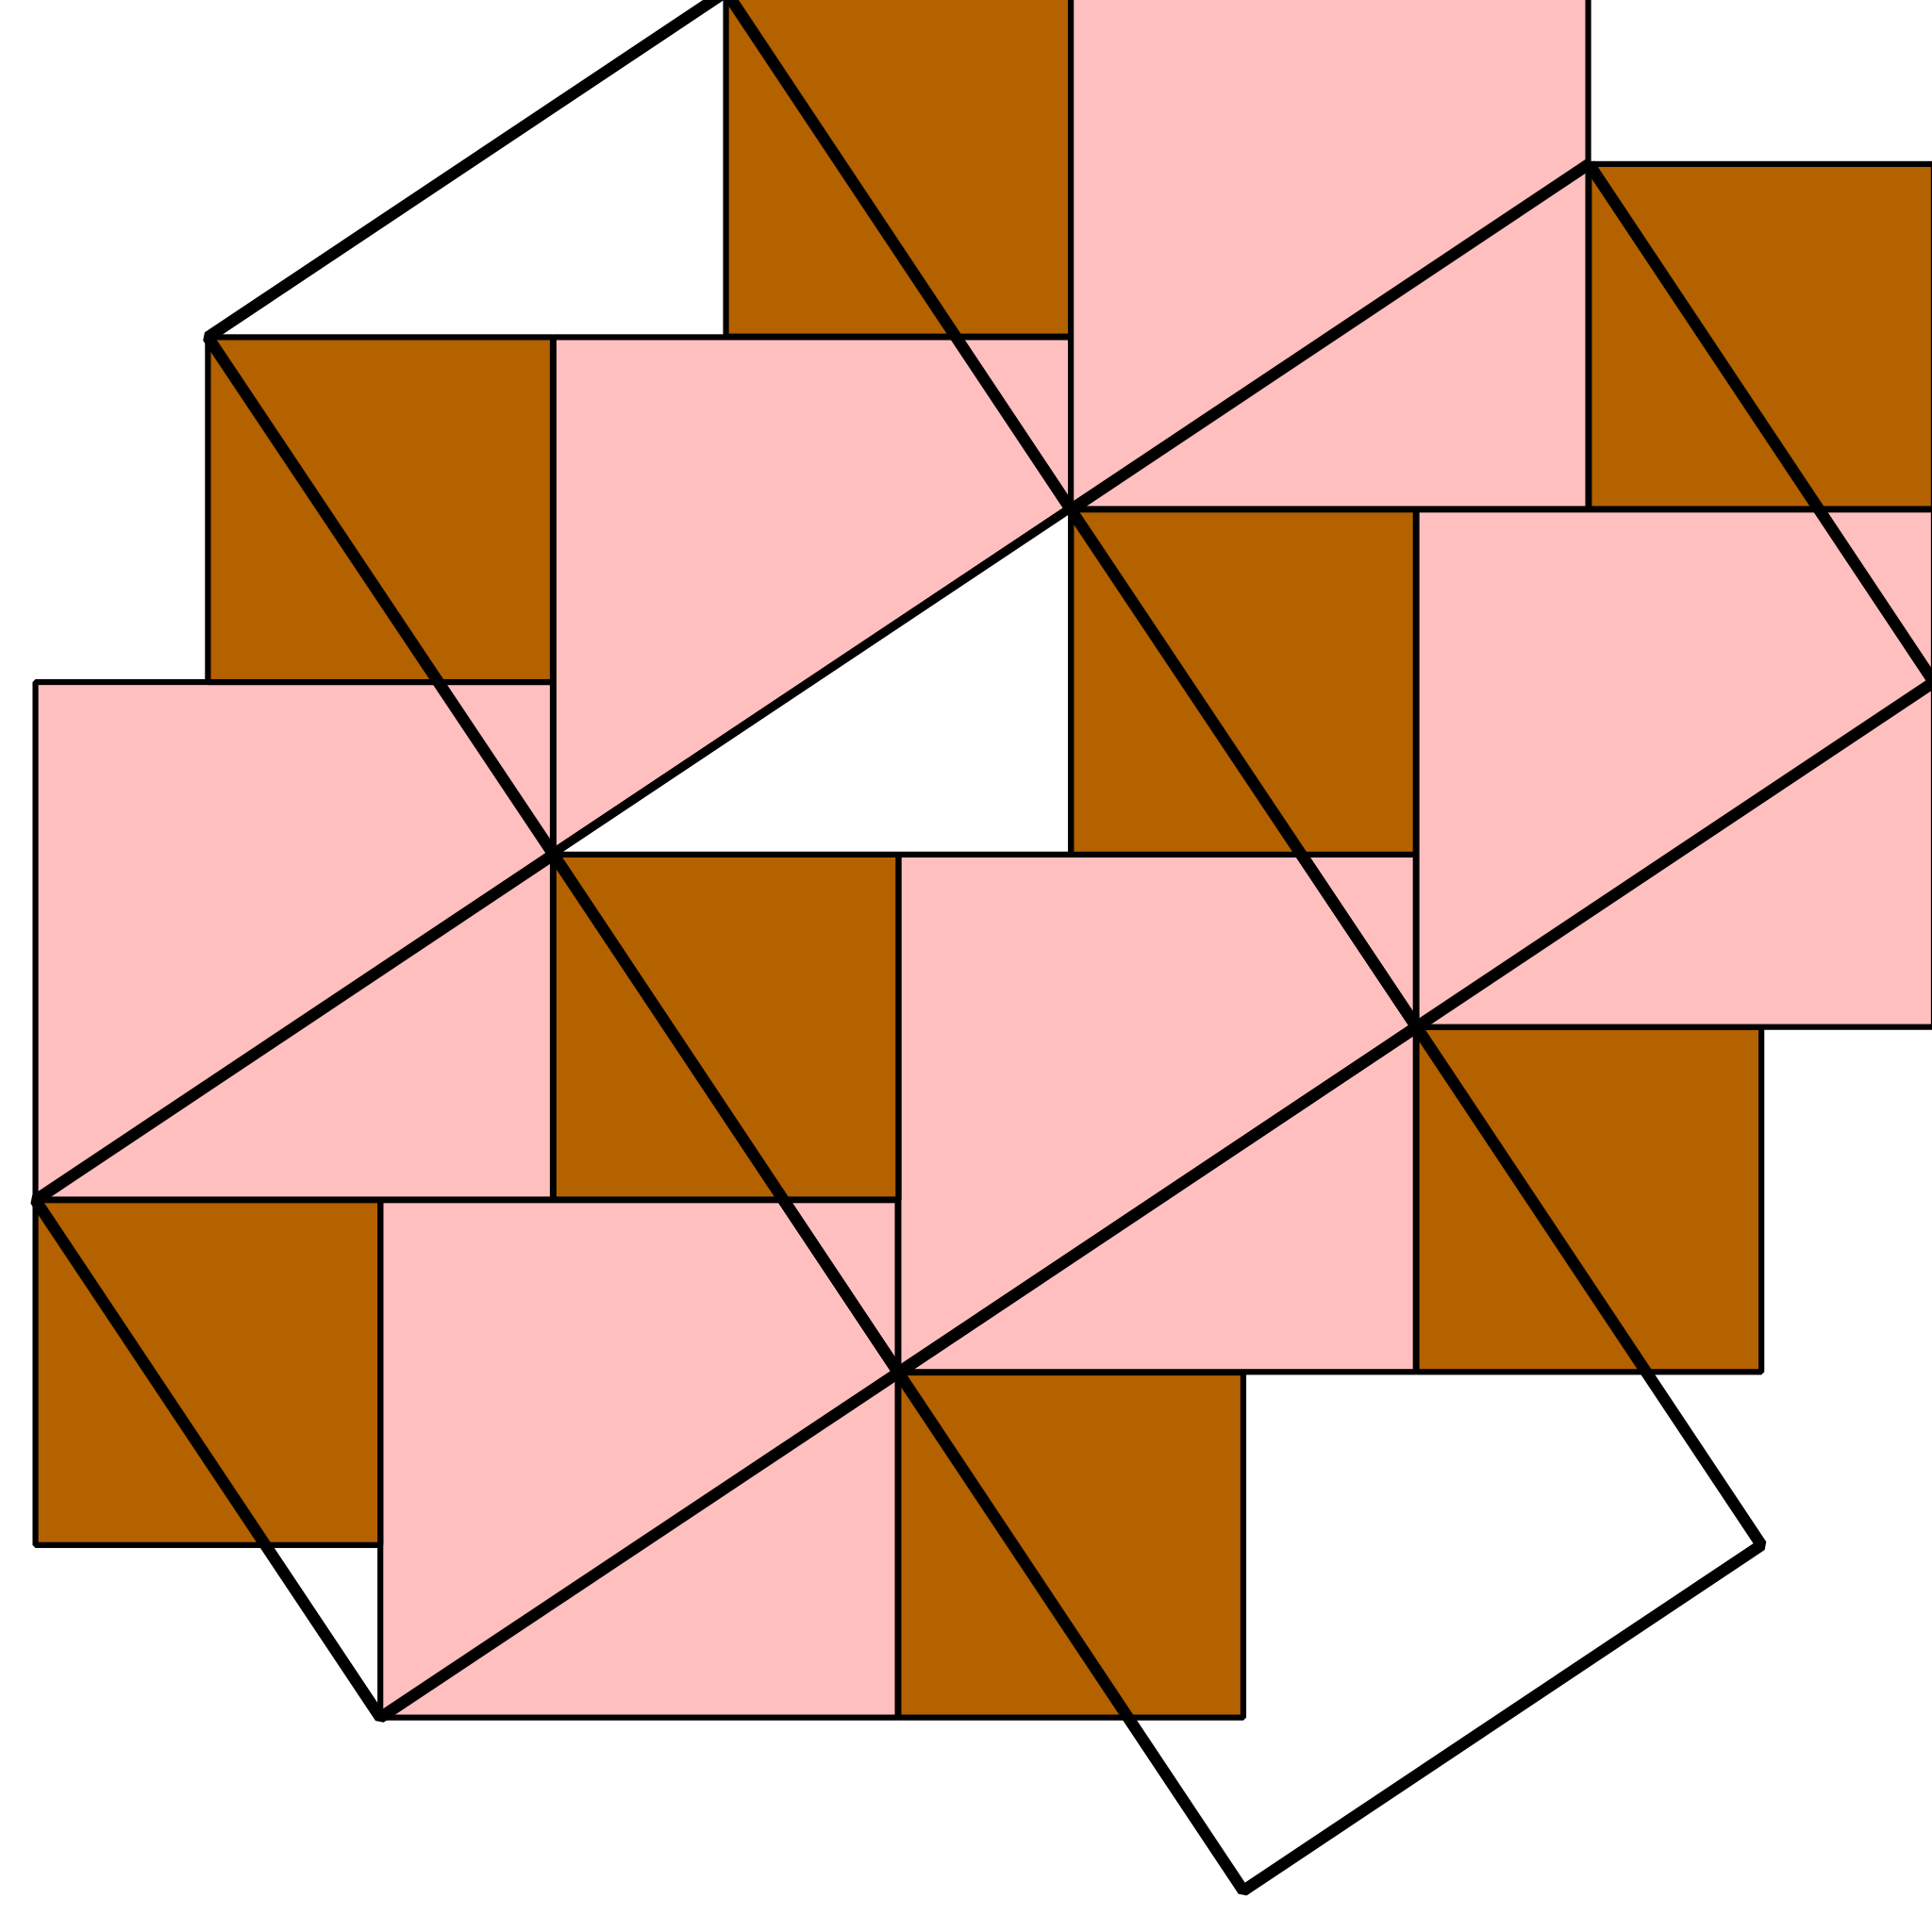
\includegraphics{../graphics/pbppyth2.pdf}
\]
\end{enumerate}
\end{problems}


\newpage



\section{Proof by Picture}
\marginnote{Most of the \textit{pictures} from this section are adapted from the wonderful source books: \cite{nelsen} and \cite{nelsen1}.}  

Pictures generally do not constitute a proof on their own. However, a
good picture can show insight and communicate concepts better than
words alone. In this section we will show you pictures giving the idea
of a proof and then ask you to supply the words to finish off the
argument. 


\subsection{Proofs Involving Right Triangles}

Let's start with something easy:

\begin{question} Explain how the following picture ``proves'' that
  the area of a right triangle is half the base times the height.
\[
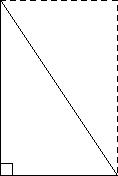
\includegraphics{../graphics/pbpAreaRight.pdf}
\]
\end{question}
\QM 

That wasn't so bad was it? Now for a game of \textit{whose-who}:

\begin{question} What is the most famous theorem in mathematics? 
\end{question}
Probably the Pythagorean Theorem comes to mind. Let's recall the statement of the Pythagorean Theorem:

\begin{theorem}[Pythagorean Theorem]\index{Pythagorean Theorem} Given a right triangle, the sum of the squares of the 
lengths of the two legs equals the square of the length of 
the hypotenuse.  Symbolically, if $a$ and $b$ represent the 
lengths of the legs and $c$ is the length of the hypotenuse, 
\[
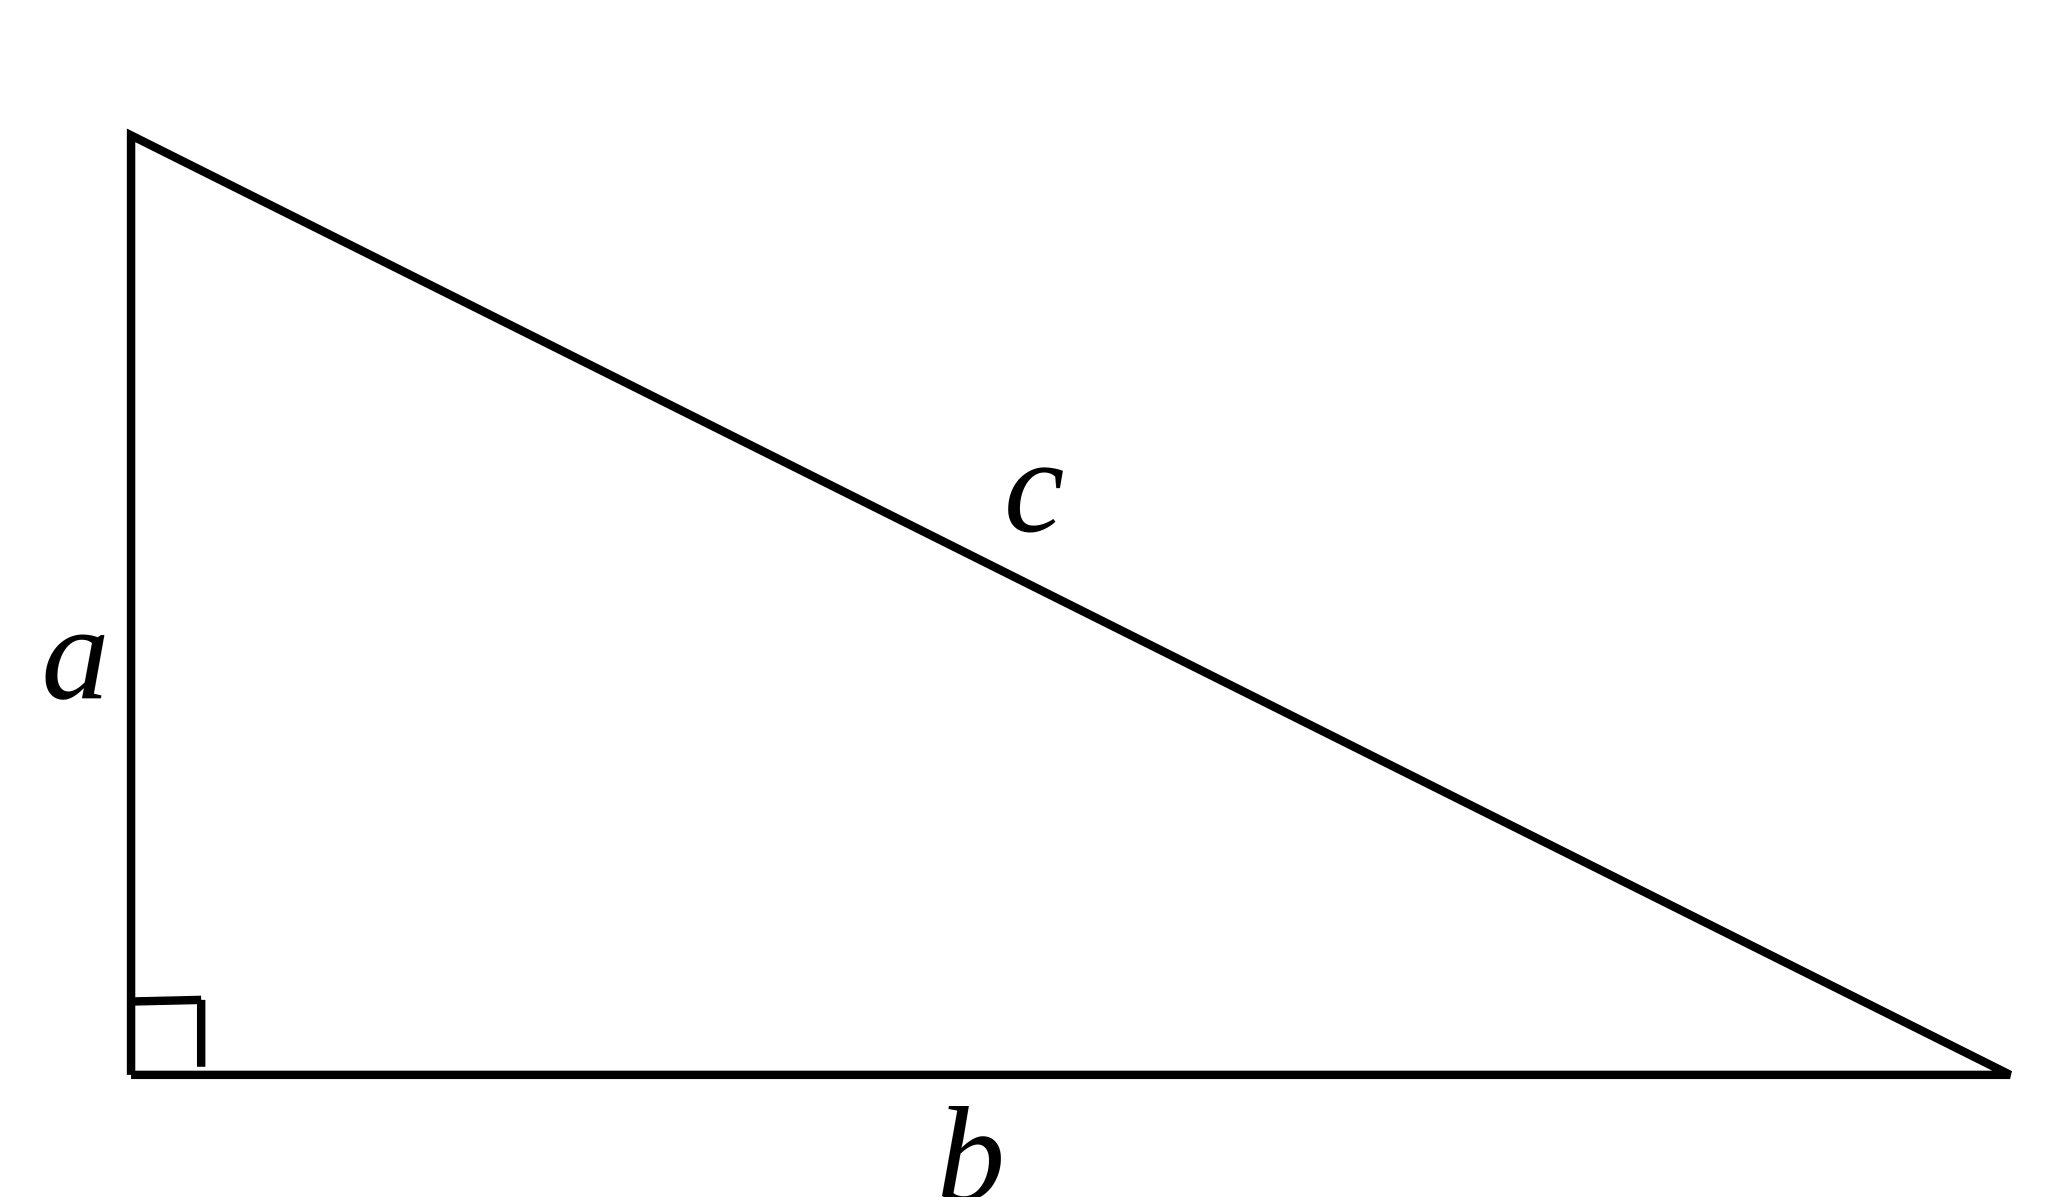
\includegraphics{../graphics/pbppyth.pdf}
\]
then 
\[
a^2 + b^2 = c^2.
\]
\end{theorem}
\begin{question} What is the converse to the Pythagorean Theorem? Is it true? How do you prove it?
\end{question}
\QM

While everyone may know the Pythagorean Theorem, not as many know how to prove it. Euclid's proof goes kind of like this: 

Consider the following picture:
\[
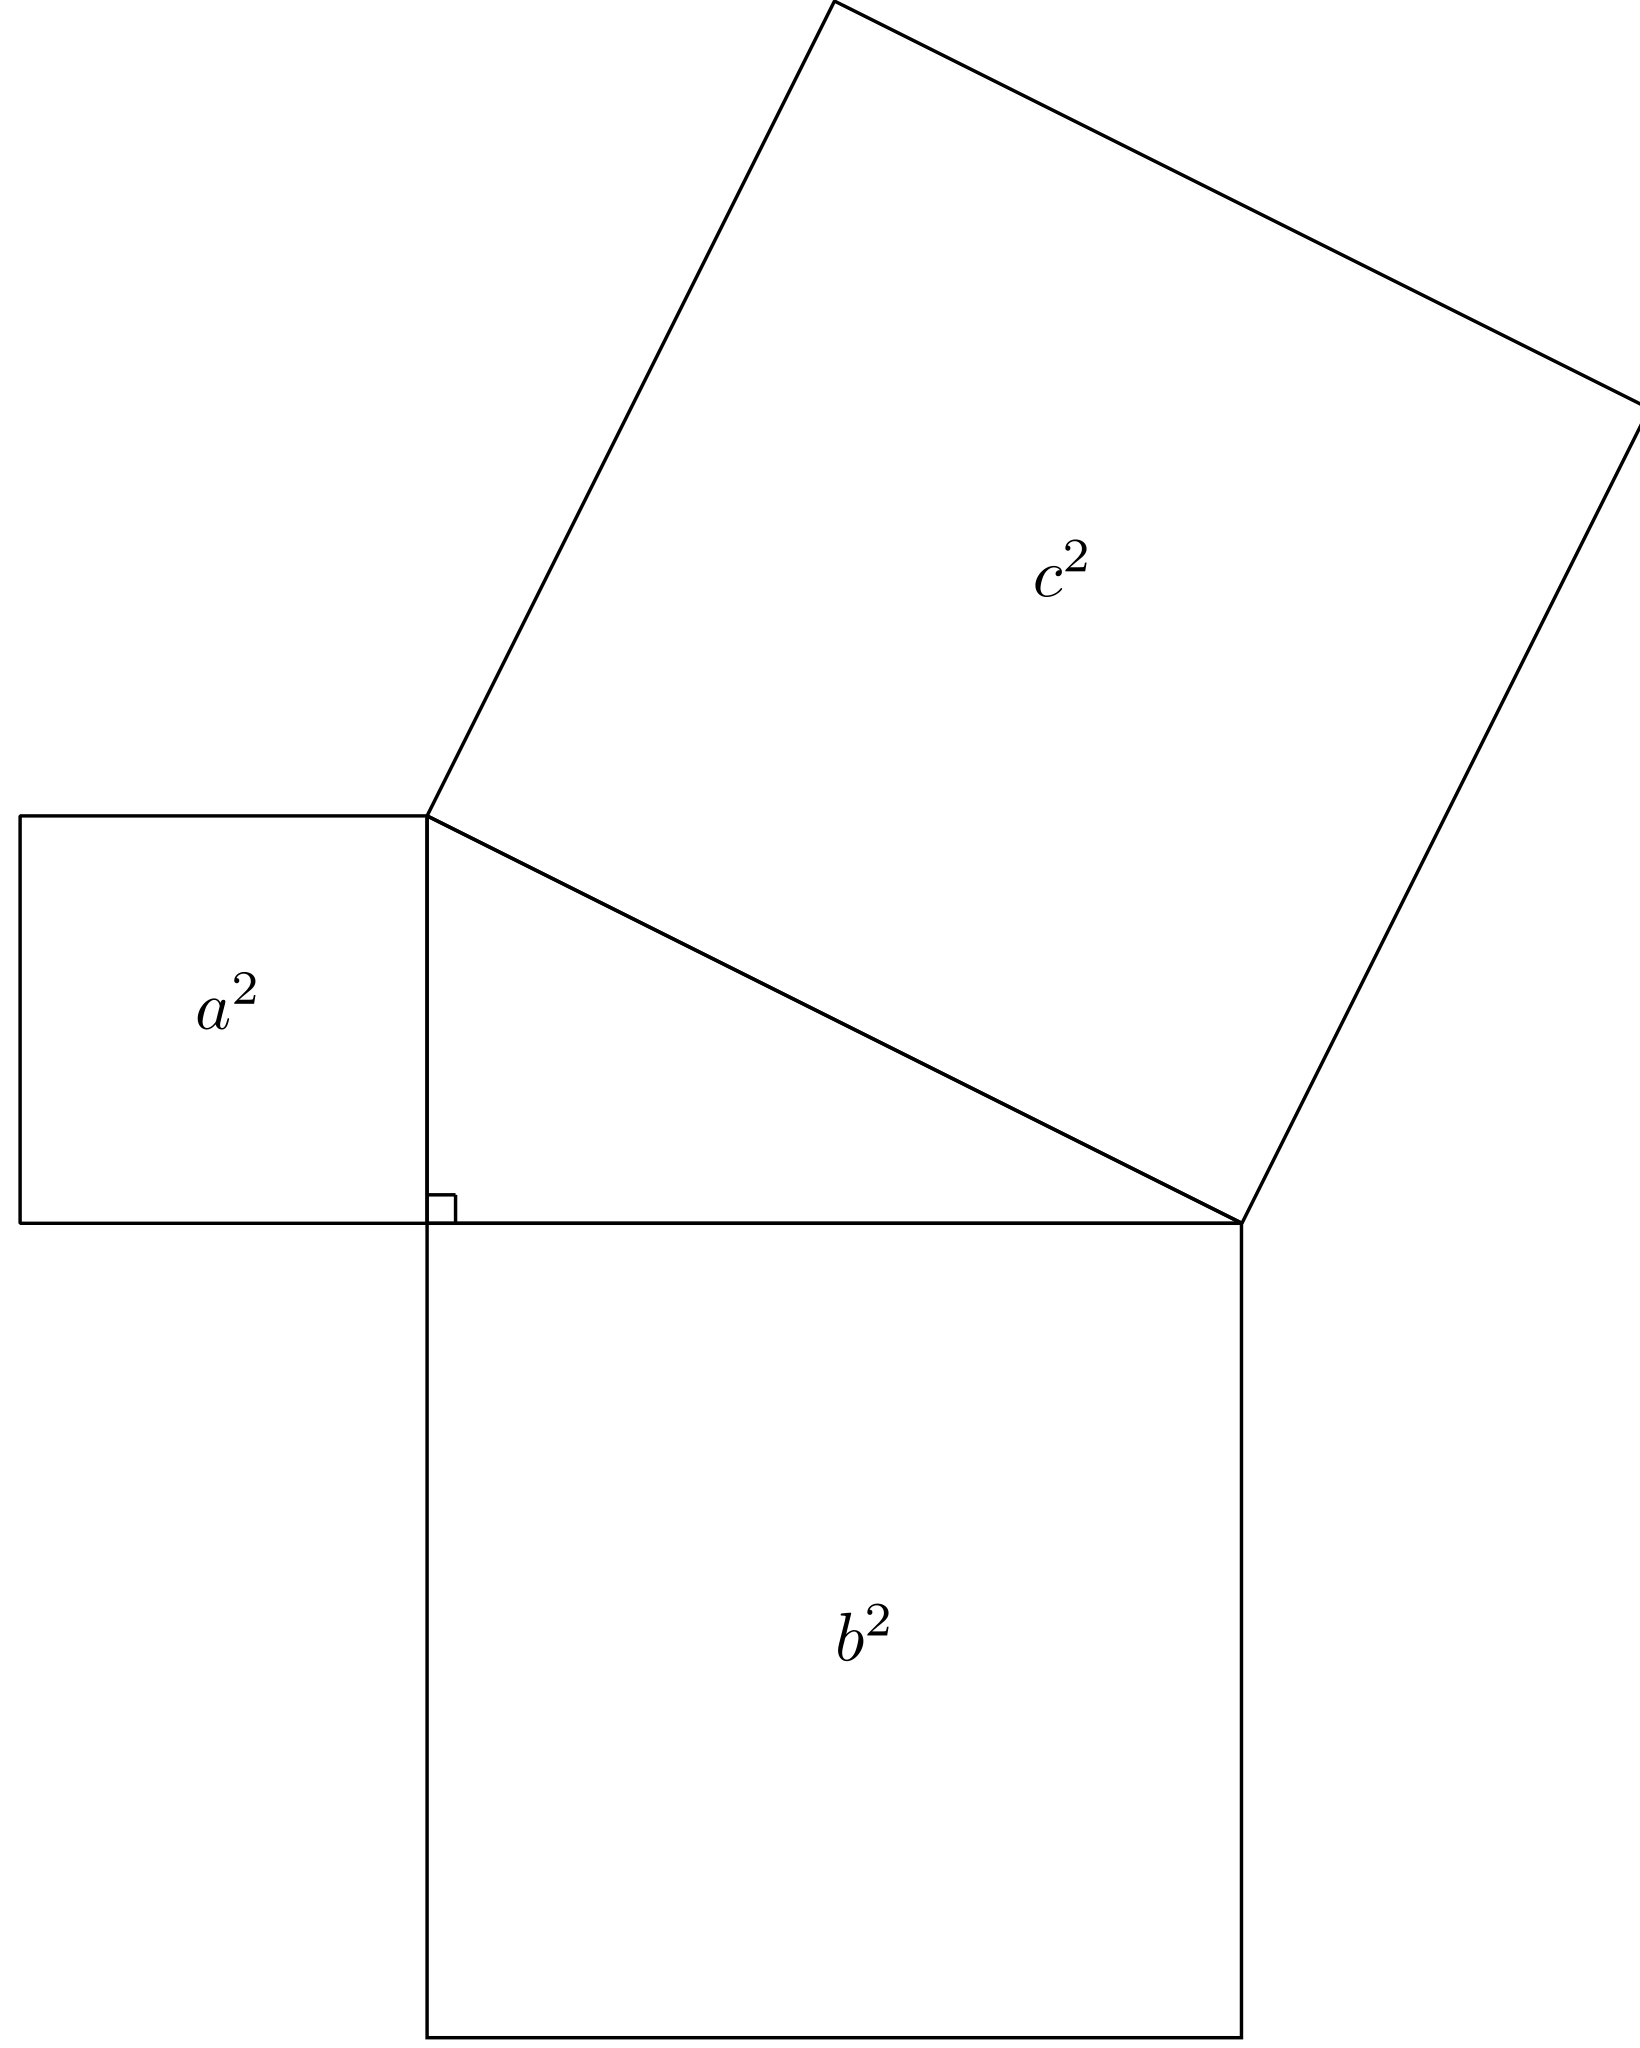
\includegraphics[scale=0.8]{../graphics/pbppythsqr.pdf}
\]
Now, cut up the squares $a^2$ and $b^2$ in such a way that they fit into $c^2$ perfectly. When you give a proof that involves cutting up the shapes and putting them back together, it is called a \textbf{dissection proof}.\index{dissection proof} The trick to ensure that this is actually a proof is in making sure
that your dissection will work no matter what right triangle you are
given. Does it sound complicated? Well it can be. 


Is there an easier proof?  Sure, look at:
\[
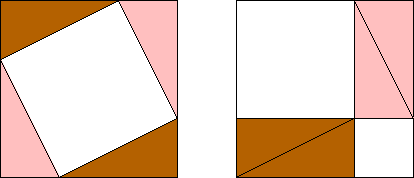
\includegraphics{../graphics/pbppyth1.pdf}
\]
\begin{question} How does the picture above ``prove'' the Pythagorean Theorem?
\end{question}


\begin{proof}[Solution] Both of the large squares above are the same size. Moreover both the unshaded regions above must have the same area. The large white square on the left has an area of $c^2$ and the two white squares on the right have a combined area of $a^2 + b^2$. Thus we see that:
\[
c^2 = a^2 + b^2
\]
\end{proof}


Now a paradox:

\begin{paradox}\index{paradox!triangle dissection} What is wrong with this picture?
\[
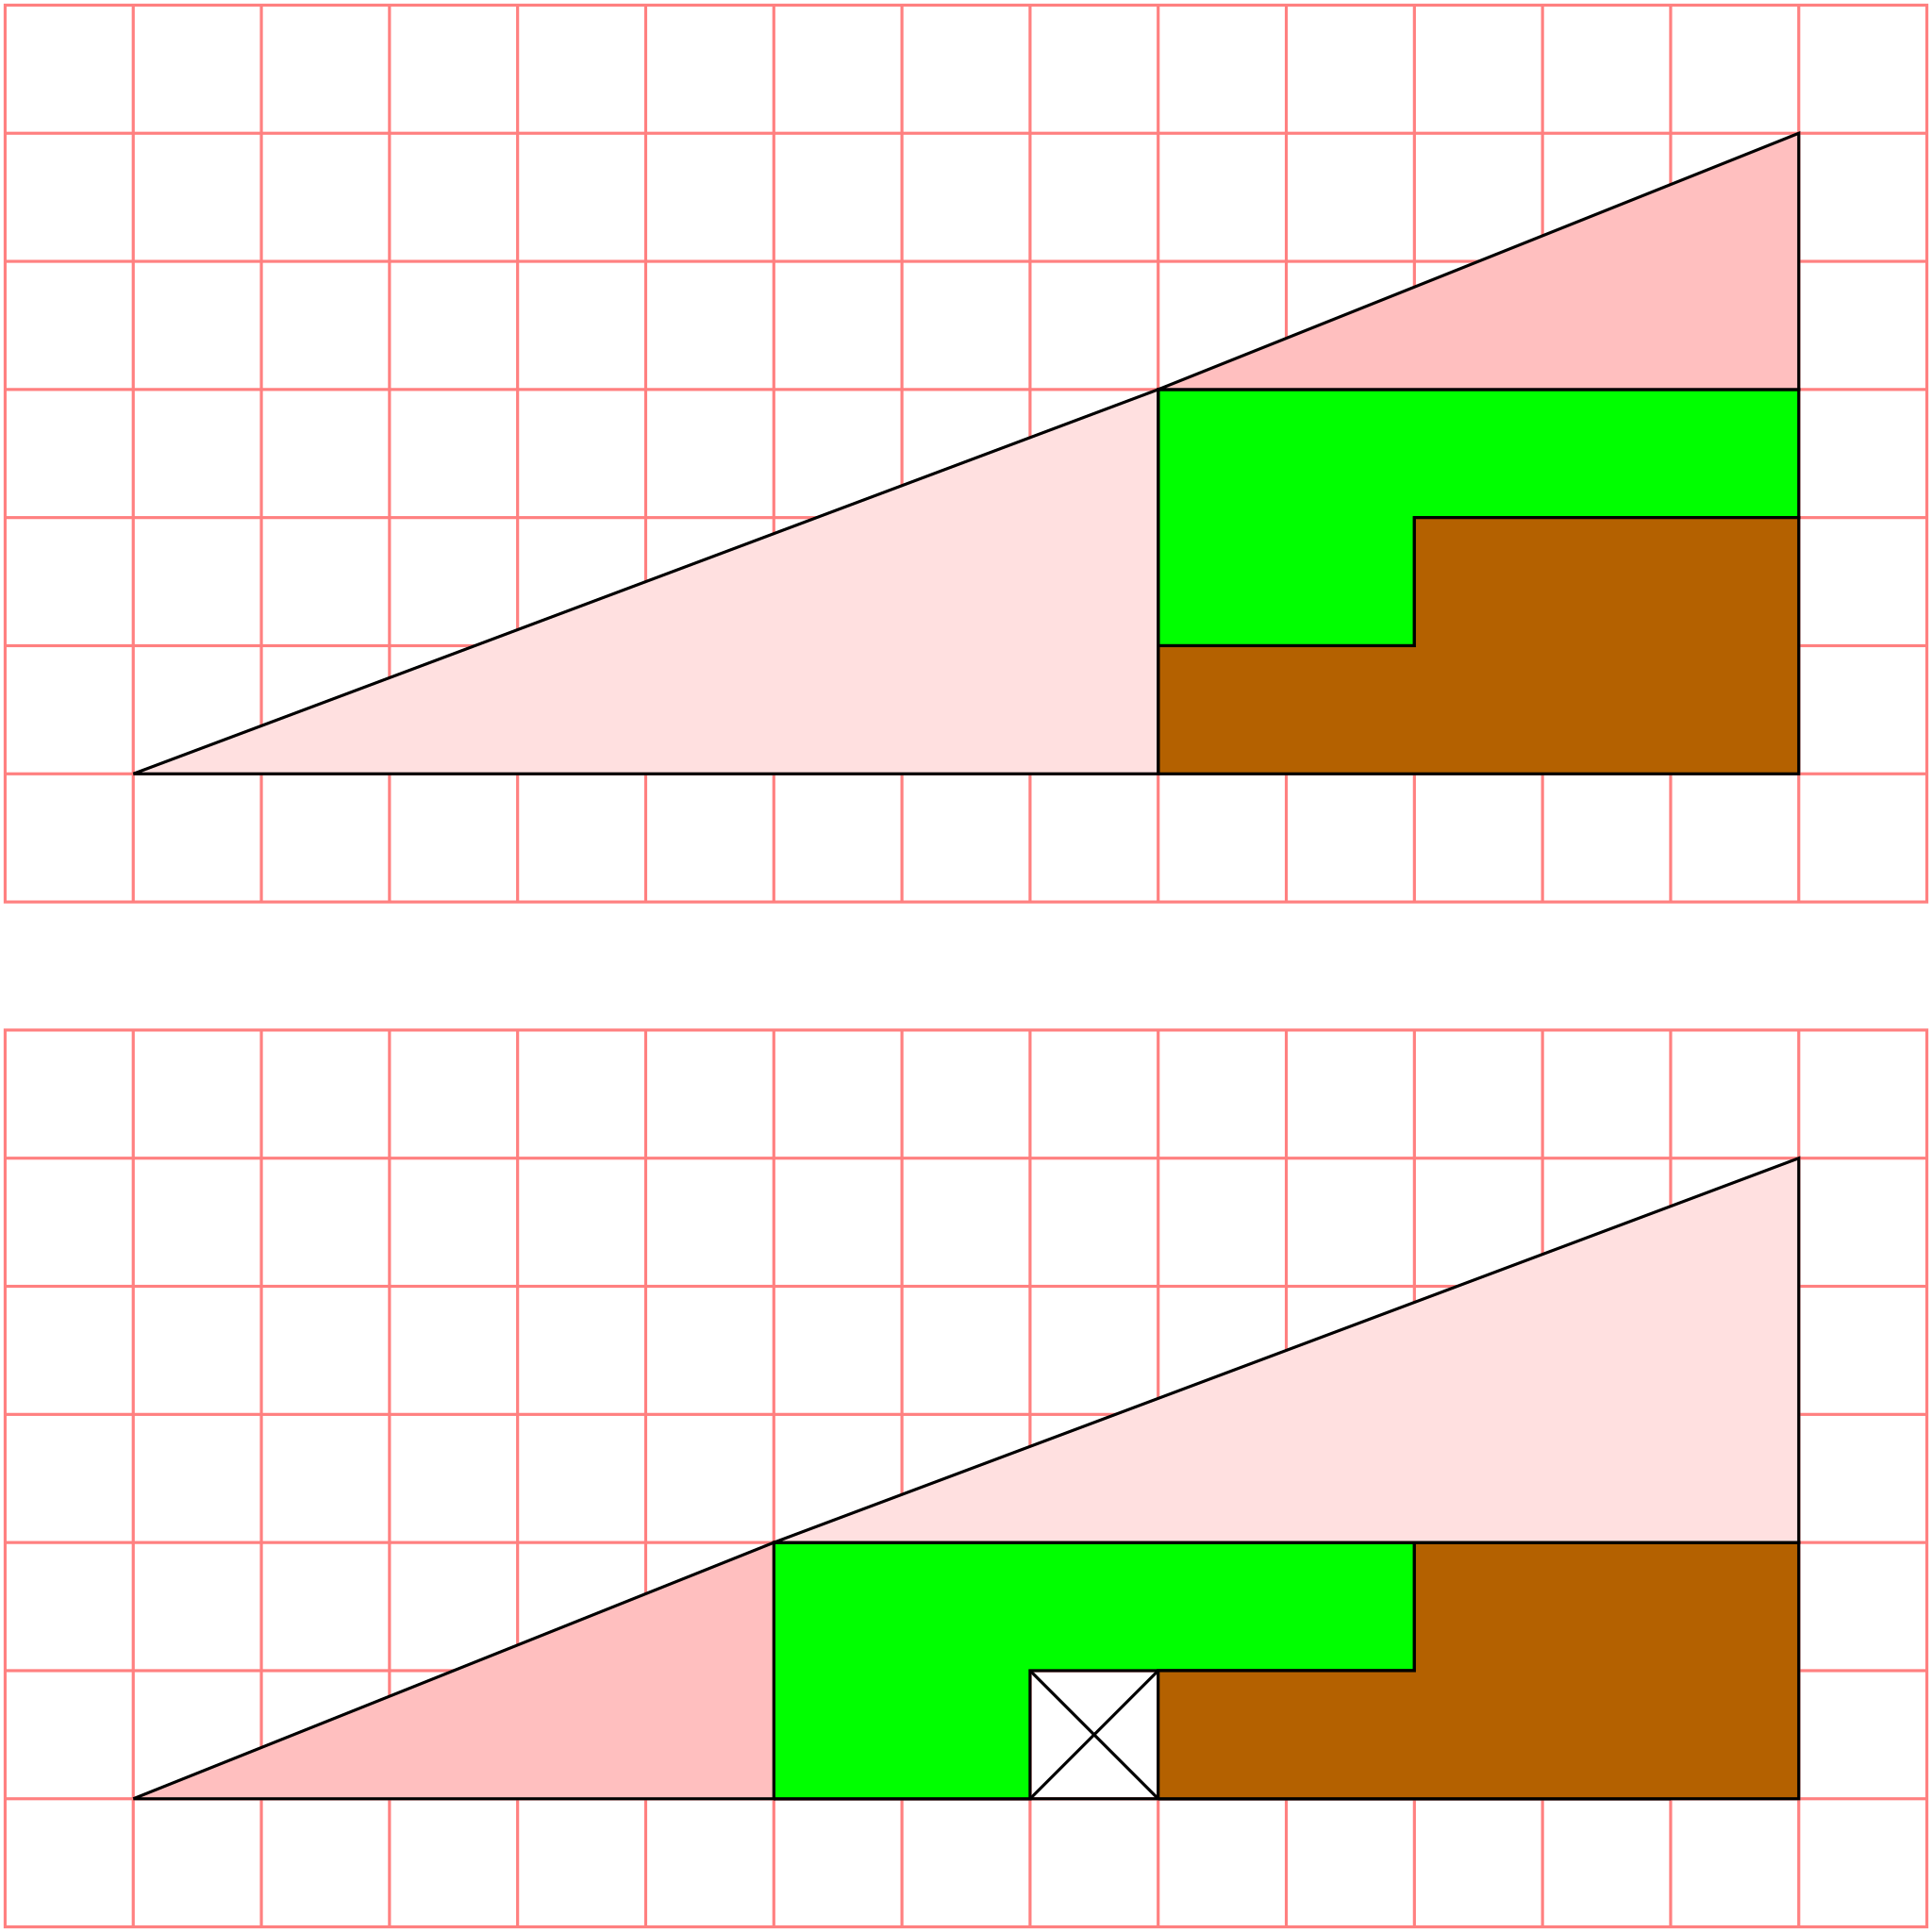
\includegraphics[scale=0.8]{../graphics/triparadox.pdf}
\]
\end{paradox}

\begin{question} 
How does this happen?   
% (See CITATION ERROR % \cite{gardner2} 
% Chapter 8, for a wonderful discussion of puzzling pictures like this one.)
\end{question}
\QM

\subsection{Proofs Involving Boxy Things}

Consider the problem of \textit{Doubling the Cube}.\index{doubling the cube} If a mathematician asks us to double a cube, he or she is asking us to double the \textbf{volume} of a given cube. One may be tempted to merely double each side, but this doesn't double the volume! 

\begin{question} Why doesn't doubling each side of the cube double the volume of the cube? 
\end{question}
\QM

Well, let's answer an easier question first. How do you double the area of a square? Does taking each side and doubling it work? 
\[
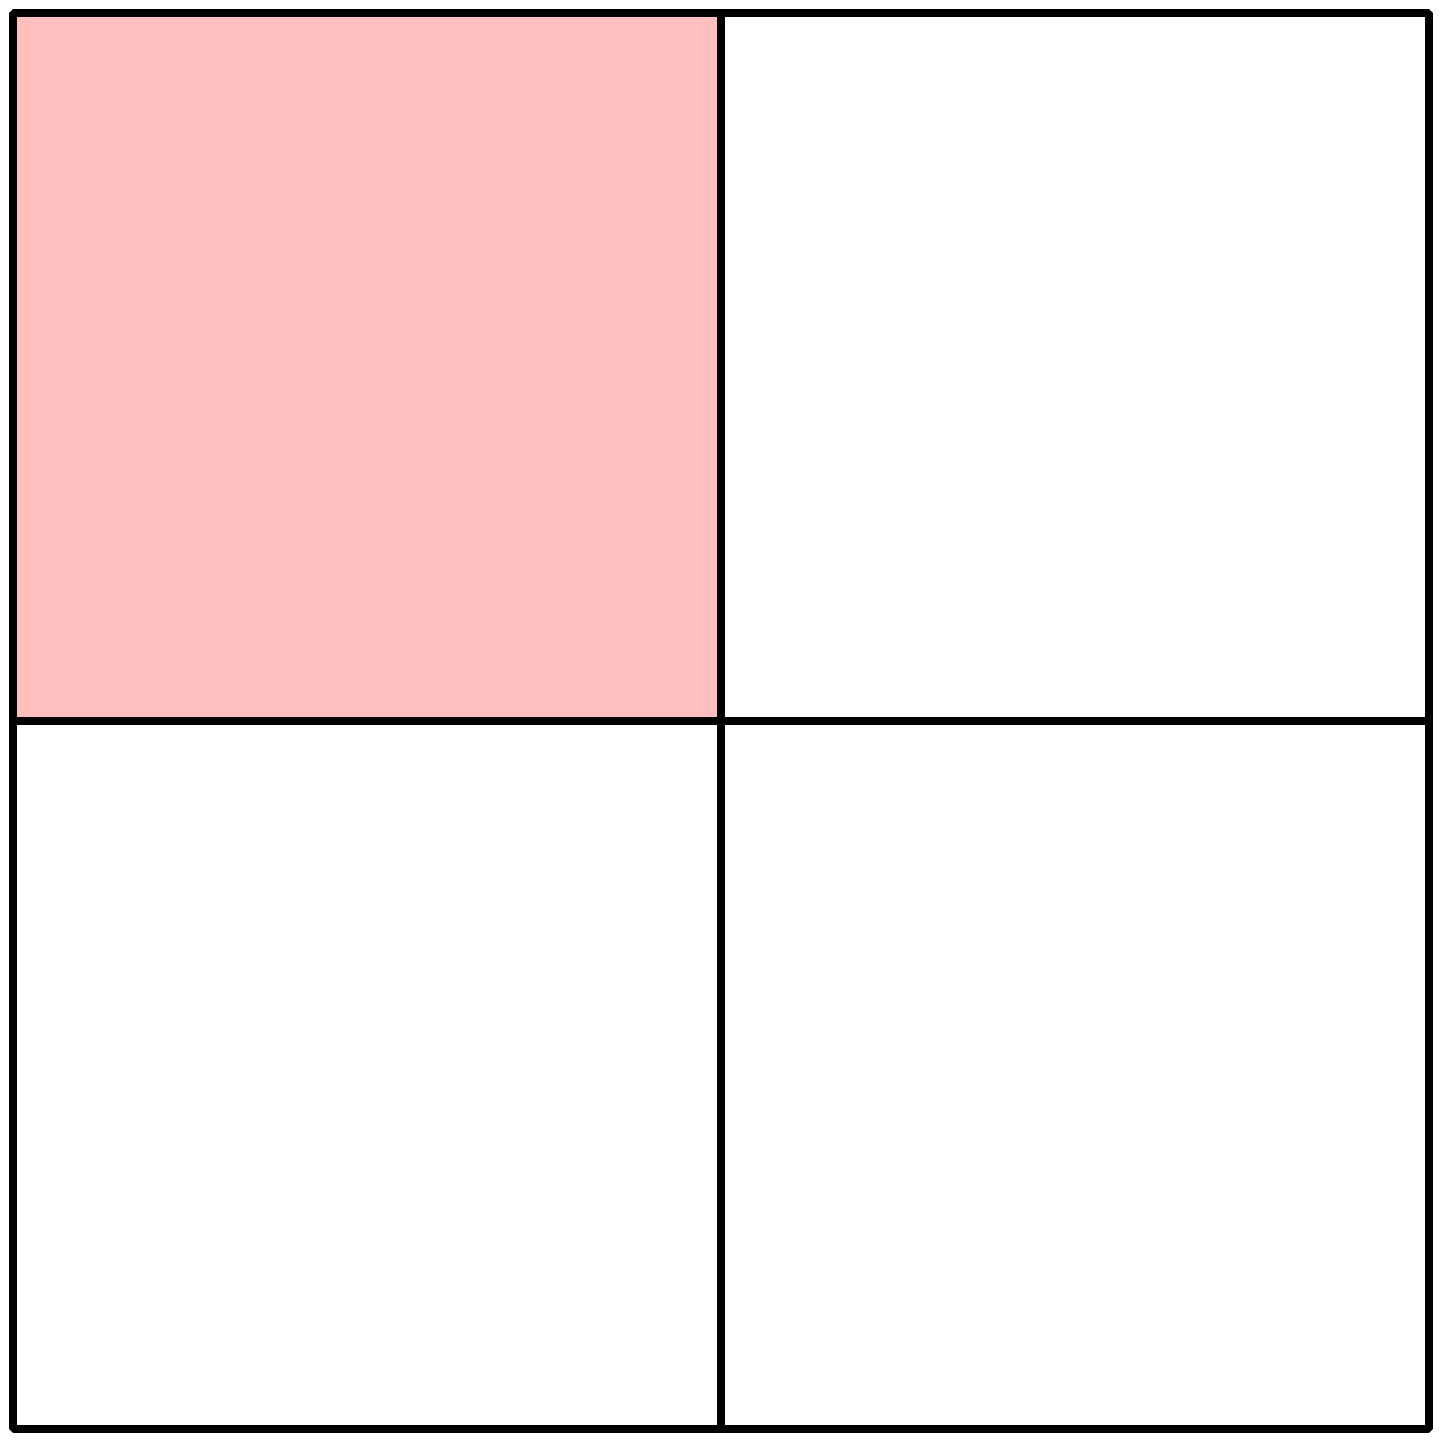
\includegraphics{../graphics/pbpsquare.pdf}
\]
No!  You now have four times the area. So you \textbf{cannot} double the area of a square merely by doubling each side.
What about for the cube? Can you double the volume of a cube merely by doubling the length of every side? Check this out:
\[
\includegraphics[scale=.4]{../graphics/119VolumeCube.pdf}
\]
Ah, so the answer is again no. If you double each side of a cube you have $8$ times the volume.

\begin{question}
What happens to the area of a square if you multiply the sides by an
arbitrary integer? What about the volume of a cube? Can you explain
what is happening here?
\end{question} 
\QM



\subsection{Proofs Involving Infinite Sums}

As is our style, we will start off with a question:

\begin{question} Can you add up an infinite number of terms and still get a 
finite number?
\end{question}


Consider $1/3$.  Actually, consider the decimal notation for $1/3$:
\[
\frac{1}{3} = .333333333333333333333333333333\dots
\]
But this is merely the sum:
\[
.3 + .03 + .003 + .0003 + .00003 + .000003 + \cdots
\]
It stays less than $1$ because the terms get so small so 
quickly.  Are there other infinite sums of this sort?  You 
bet! Check out this picture:
\[
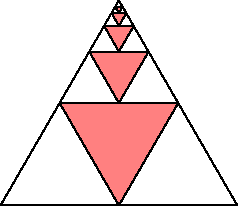
\includegraphics{../graphics/pbptriangle.pdf}
\]
\begin{question} Explain how the picture above ``proves'' that:
\[
\frac{1}{4} + \left(\frac{1}{4}\right)^2 +  \left(\frac{1}{4}\right)^3 +  \left(\frac{1}{4}\right)^4 +  \left(\frac{1}{4}\right)^5 + \cdots = \frac{1}{3}
\]
\end{question}

\begin{proof}[Solution] Let's take it in steps.  If the big triangle has area 
$1$, the area of the shaded region below is $1/4$. 
\[
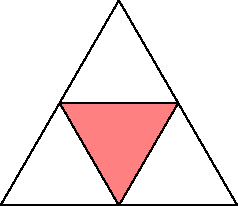
\includegraphics{../graphics/pbptriangle1.pdf}
\]
We also see that the area of the shaded region below 
\[
\includegraphics{../graphics/pbptriangle2.pdf}
\]
is:
\[
\frac{1}{4} + \left(\frac{1}{4}\right)^2
\]
Continuing on in this fashion we see that the area of all the shaded regions is:
\[
\frac{1}{4} + \left(\frac{1}{4}\right)^2 +  \left(\frac{1}{4}\right)^3 +  \left(\frac{1}{4}\right)^4 +  \left(\frac{1}{4}\right)^5 + \cdots
\]
But look, the unshaded triangles have twice as much area as 
the shaded triangle.  Thus the shaded triangles must have an
area of $1/3$.
\end{proof}



\subsection{Thinking Outside the Box}


A \textit{calisson}\index{calisson} is a French candy that sort of looks like two equilateral triangles stuck together. They usually come in a hexagon-shaped box. 

\begin{question} How do the calissons fit into their hexagon-shaped box?
\end{question}

If you start to put the calissons into a box, you quickly see that they can be placed in there with exactly three different orientations:
\[
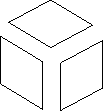
\includegraphics{../graphics/pbporicas.pdf}
\]
\begin{theorem}\label{T:cal} In any packing, the number of calissons with a given orientation is exactly one-third the total number of calissons in the box.
\end{theorem}

Look at this picture:
\[
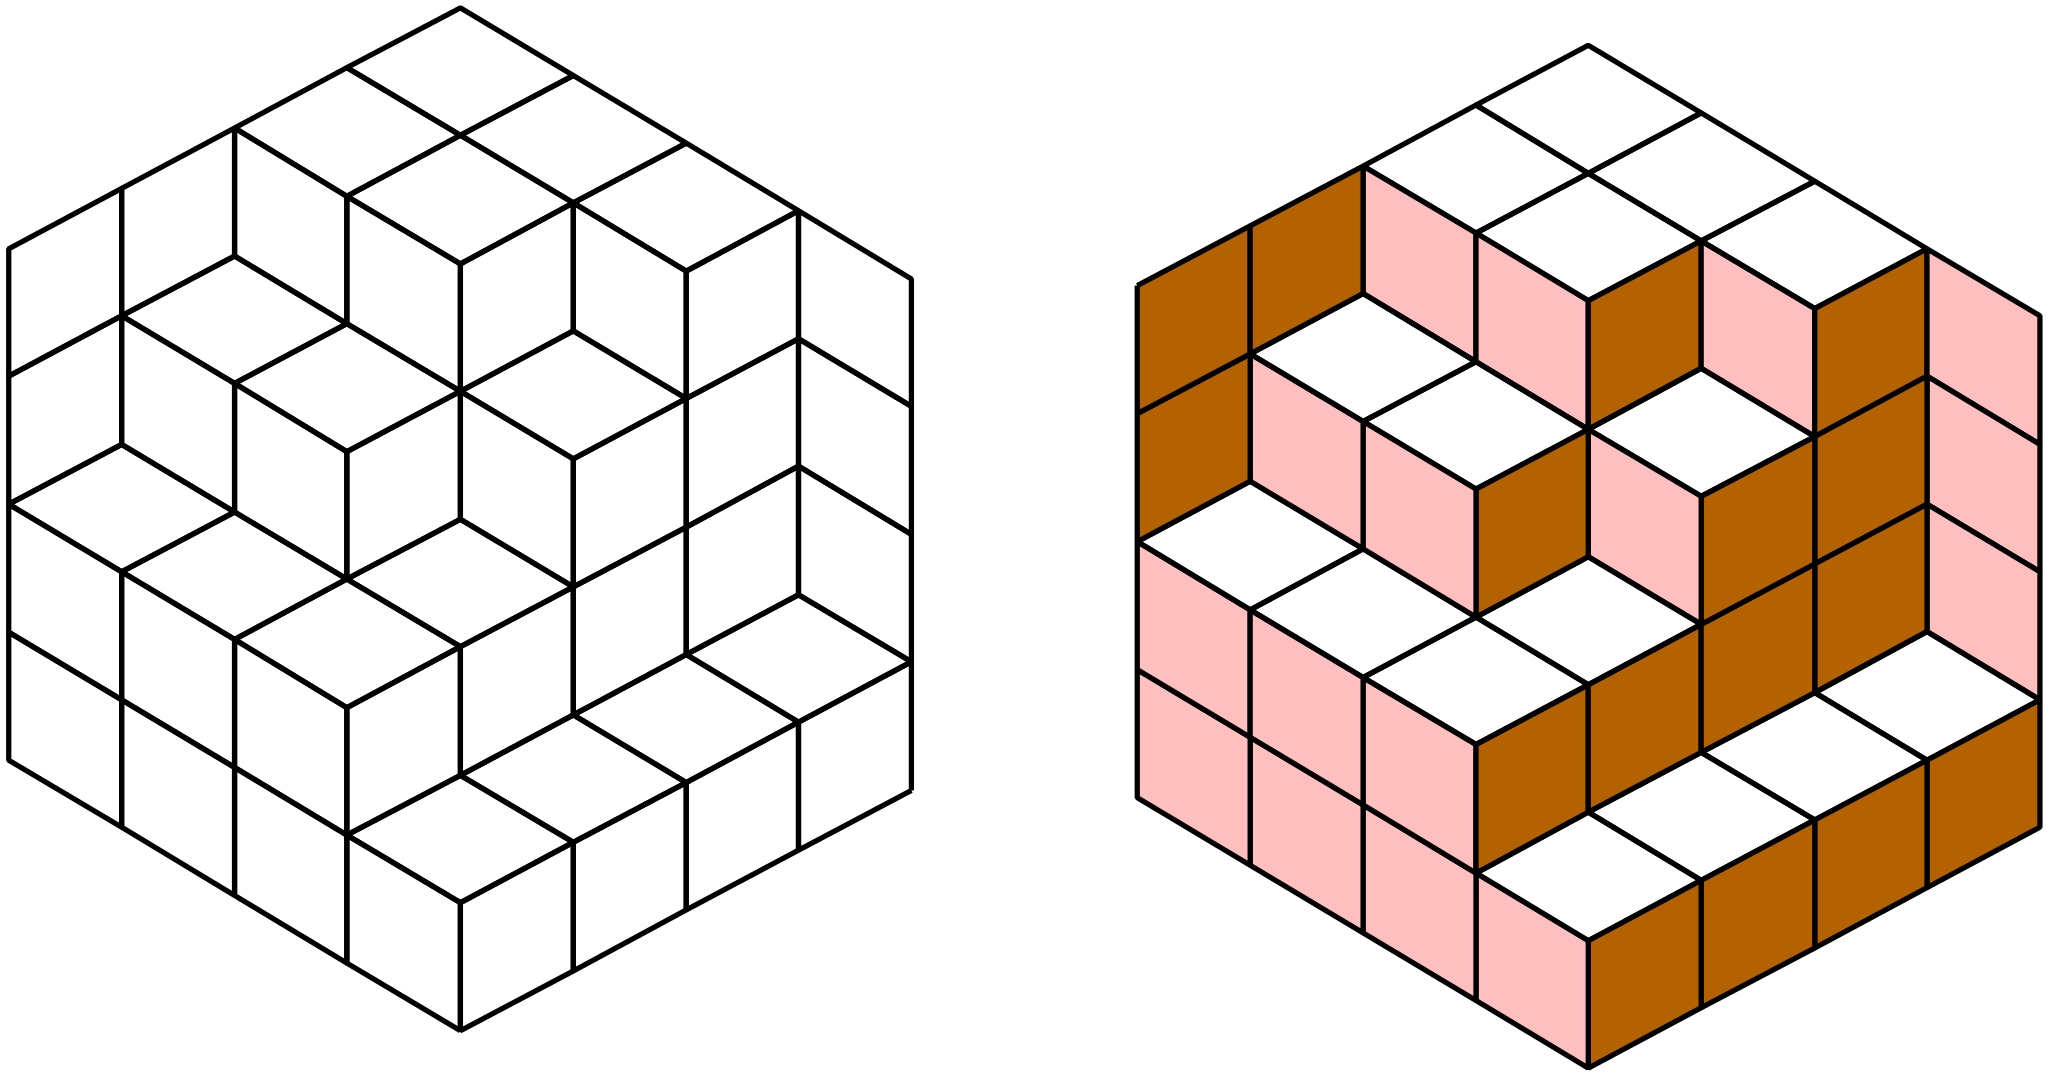
\includegraphics{../graphics/pbpcas.pdf}
\]

\begin{question} How does the picture above ``prove'' Theorem~\ref{T:cal}? Hint: Think outside the box!
\end{question}
\QM




\begin{problems}
\begin{enumerate}
\item Explain the rule
\[
\text{even} + \text{even} = \text{even}
\]
in two different ways. First give an explanation based on
pictures. Second give an explanation based on algebra. 
\item Explain the rule
\[
\text{odd} + \text{even} = \text{odd}
\]
in two different ways. First give an explanation based on
pictures. Second give an explanation based on algebra.
\item Explain the rule
\[
\text{odd} + \text{odd} = \text{even}
\]
in two different ways. First give an explanation based on
pictures. Second give an explanation based on algebra.
\item Explain the rule
\[
\text{even} \cdot \text{even} = \text{even}
\]
in two different ways. First give an explanation based on
pictures. Second give an explanation based on algebra.
\item Explain the rule
\[
\text{odd} \cdot \text{odd} = \text{odd}
\]
in two different ways. First give an explanation based on
pictures. Second give an explanation based on algebra.
\item Explain the rule
\[
\text{odd} \cdot \text{even} = \text{even}
\]
in two different ways. First give an explanation based on
pictures. Second give an explanation based on algebra.
\item\label{P:RTA} Explain how the following picture ``proves'' that
  the area of a right triangle is half the base times the height.
\[
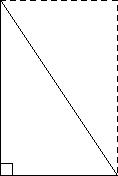
\includegraphics{../graphics/pbpAreaRight.pdf}
\]

\item Suppose you know that the area of a \textbf{right} triangle is
  half the base times the height. Explain how the following picture
  ``proves'' that the area of \textbf{every} triangle is half the base times the
  height.
\[
\includegraphics{../graphics/pbpDisTri.pdf}
\]
Now suppose that a student, say \textit{Geometry Giorgio} attempts to
solve a similar problem. Again knowing that the area of a right
triangle is half the base times the height, he draws the following
picture:
\[
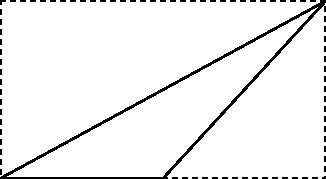
\includegraphics{../graphics/pbpDisTriGio.pdf}
\]
\textit{Geometry Giorgio} states that the diagonal line cuts the
rectangle in half, and thus the area of the triangle is half the base
times the height. Is this correct reasoning? If so, give a complete
explanation. If not, give correct reasoning based on \textit{Geometry
  Giorgio}'s picture.


\item Suppose you know that the area of a \textbf{right} triangle is
  half the base times the height. Explain how the following picture
  ``proves'' that the area of any triangle is half the base times the
  height. Note, this way of thinking is the basis for Cavalieri's
  Principle.\index{Cavalieri's Principle}
\[
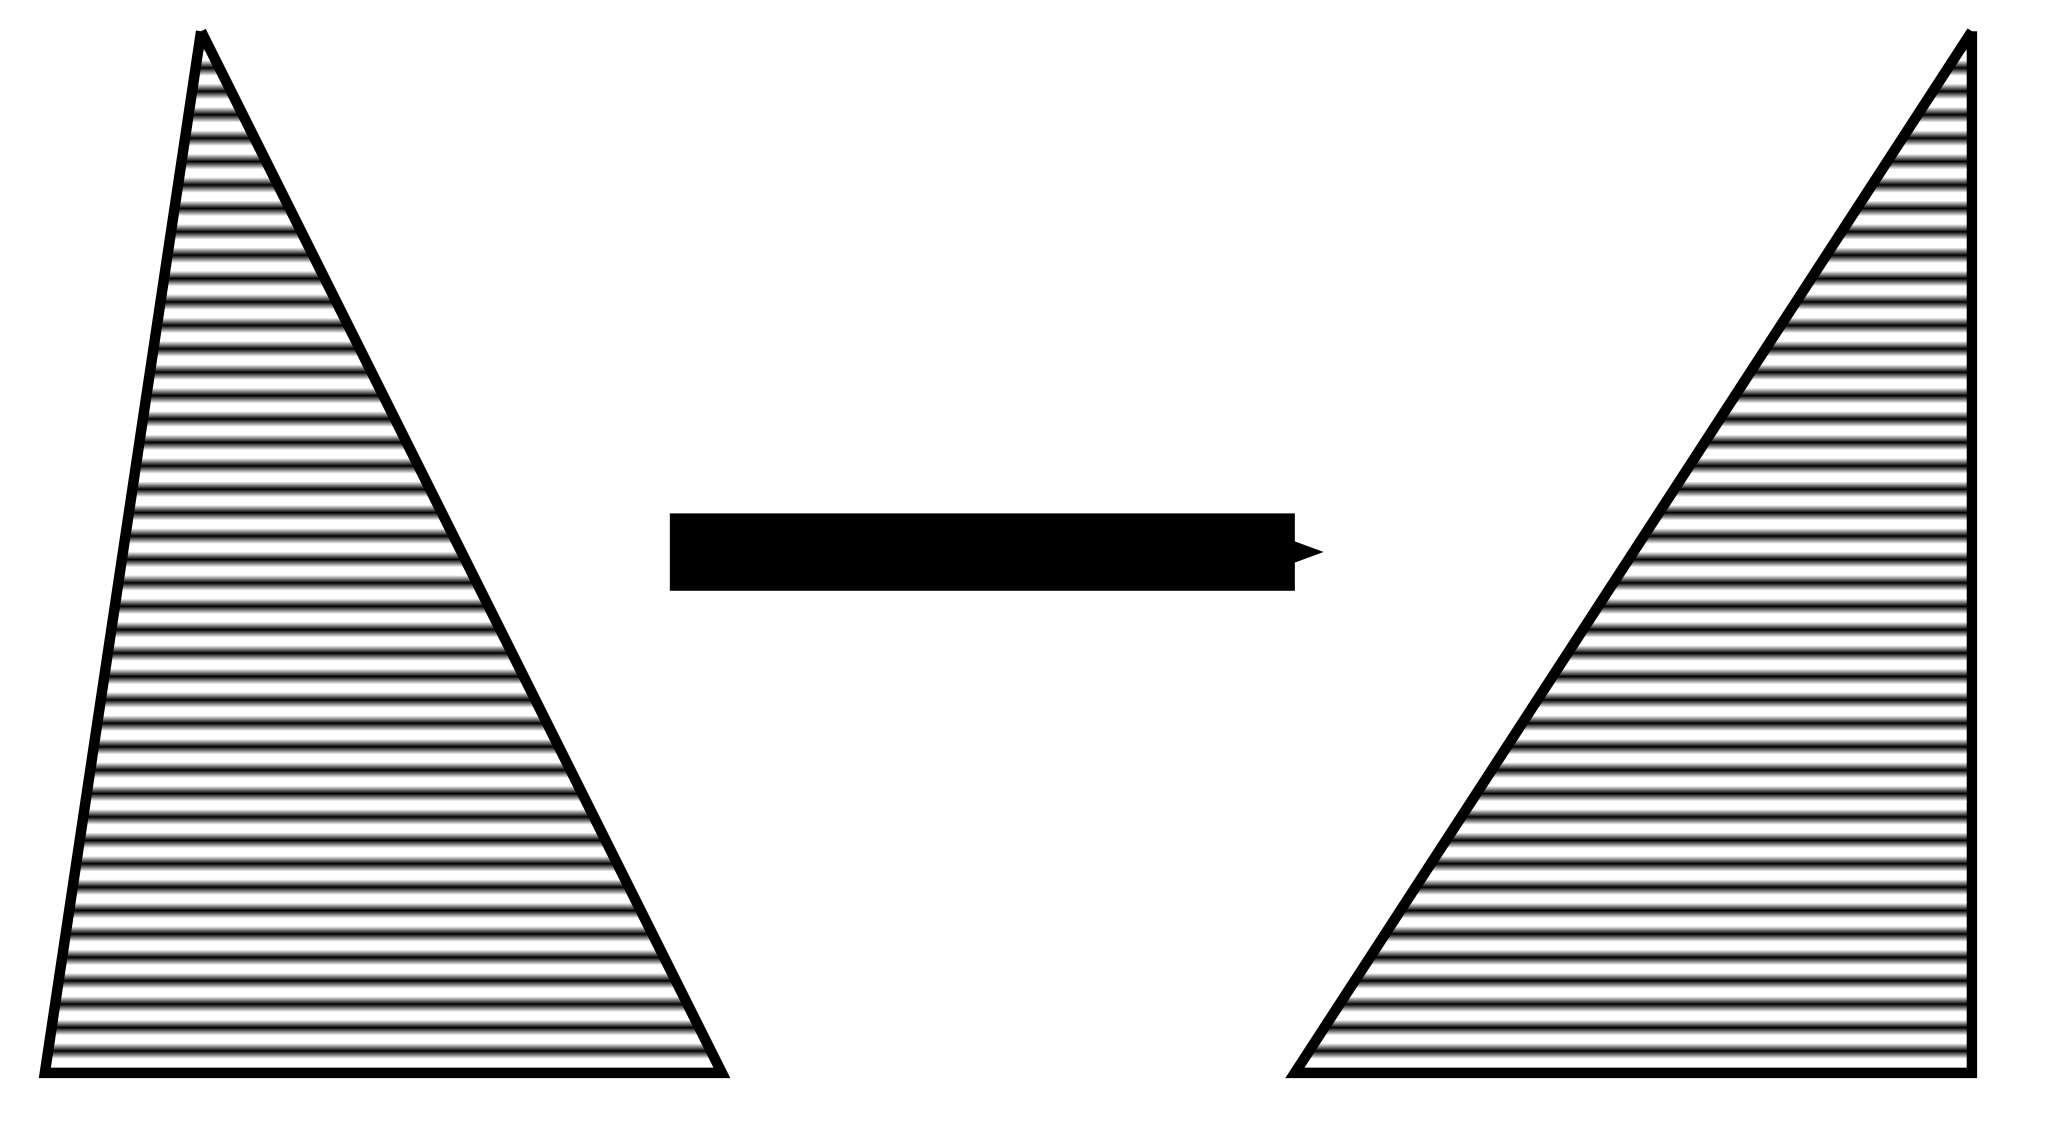
\includegraphics{../graphics/pbpShearTri.pdf}
\]
\item Explain how the following picture ``proves'' that the area of
  any parallelogram is base times height. Note, this way of thinking
  is the basis for Cavalieri's Principle.\index{Cavalieri's Principle}
\[
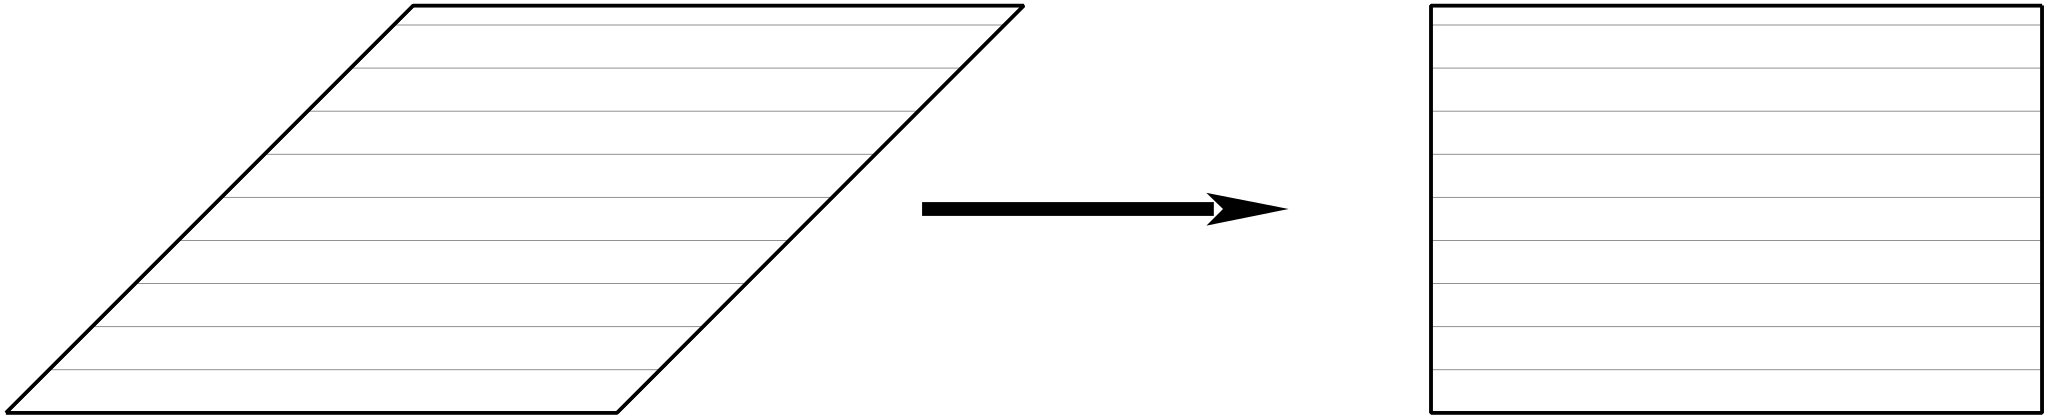
\includegraphics{../graphics/pbpShearPara.pdf}
\]

\item Explain how to use a picture to ``prove'' that a triangle of a
  given area could have an arbitrarily large perimeter.

\item Give two explanations of how the following picture ``proves''
  the Pythagorean Theorem, one using algebra and one without algebra. 
\[
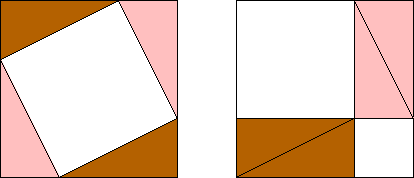
\includegraphics{../graphics/pbppyth1.pdf}
\]
\item Give two explanations of how the following picture ``proves''
  the Pythagorean Theorem, one using algebra and one without algebra. 
\[
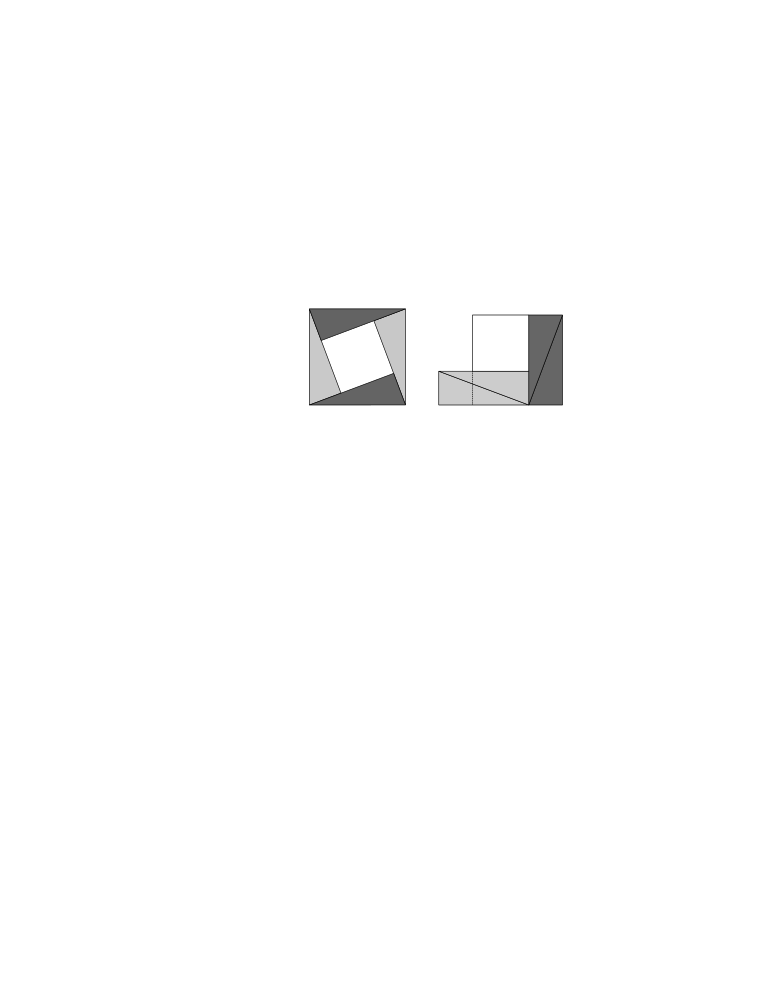
\includegraphics{../graphics/pbppyth3.pdf}
\]
\item Explain how the following picture ``proves'' the Pythagorean Theorem.
\[
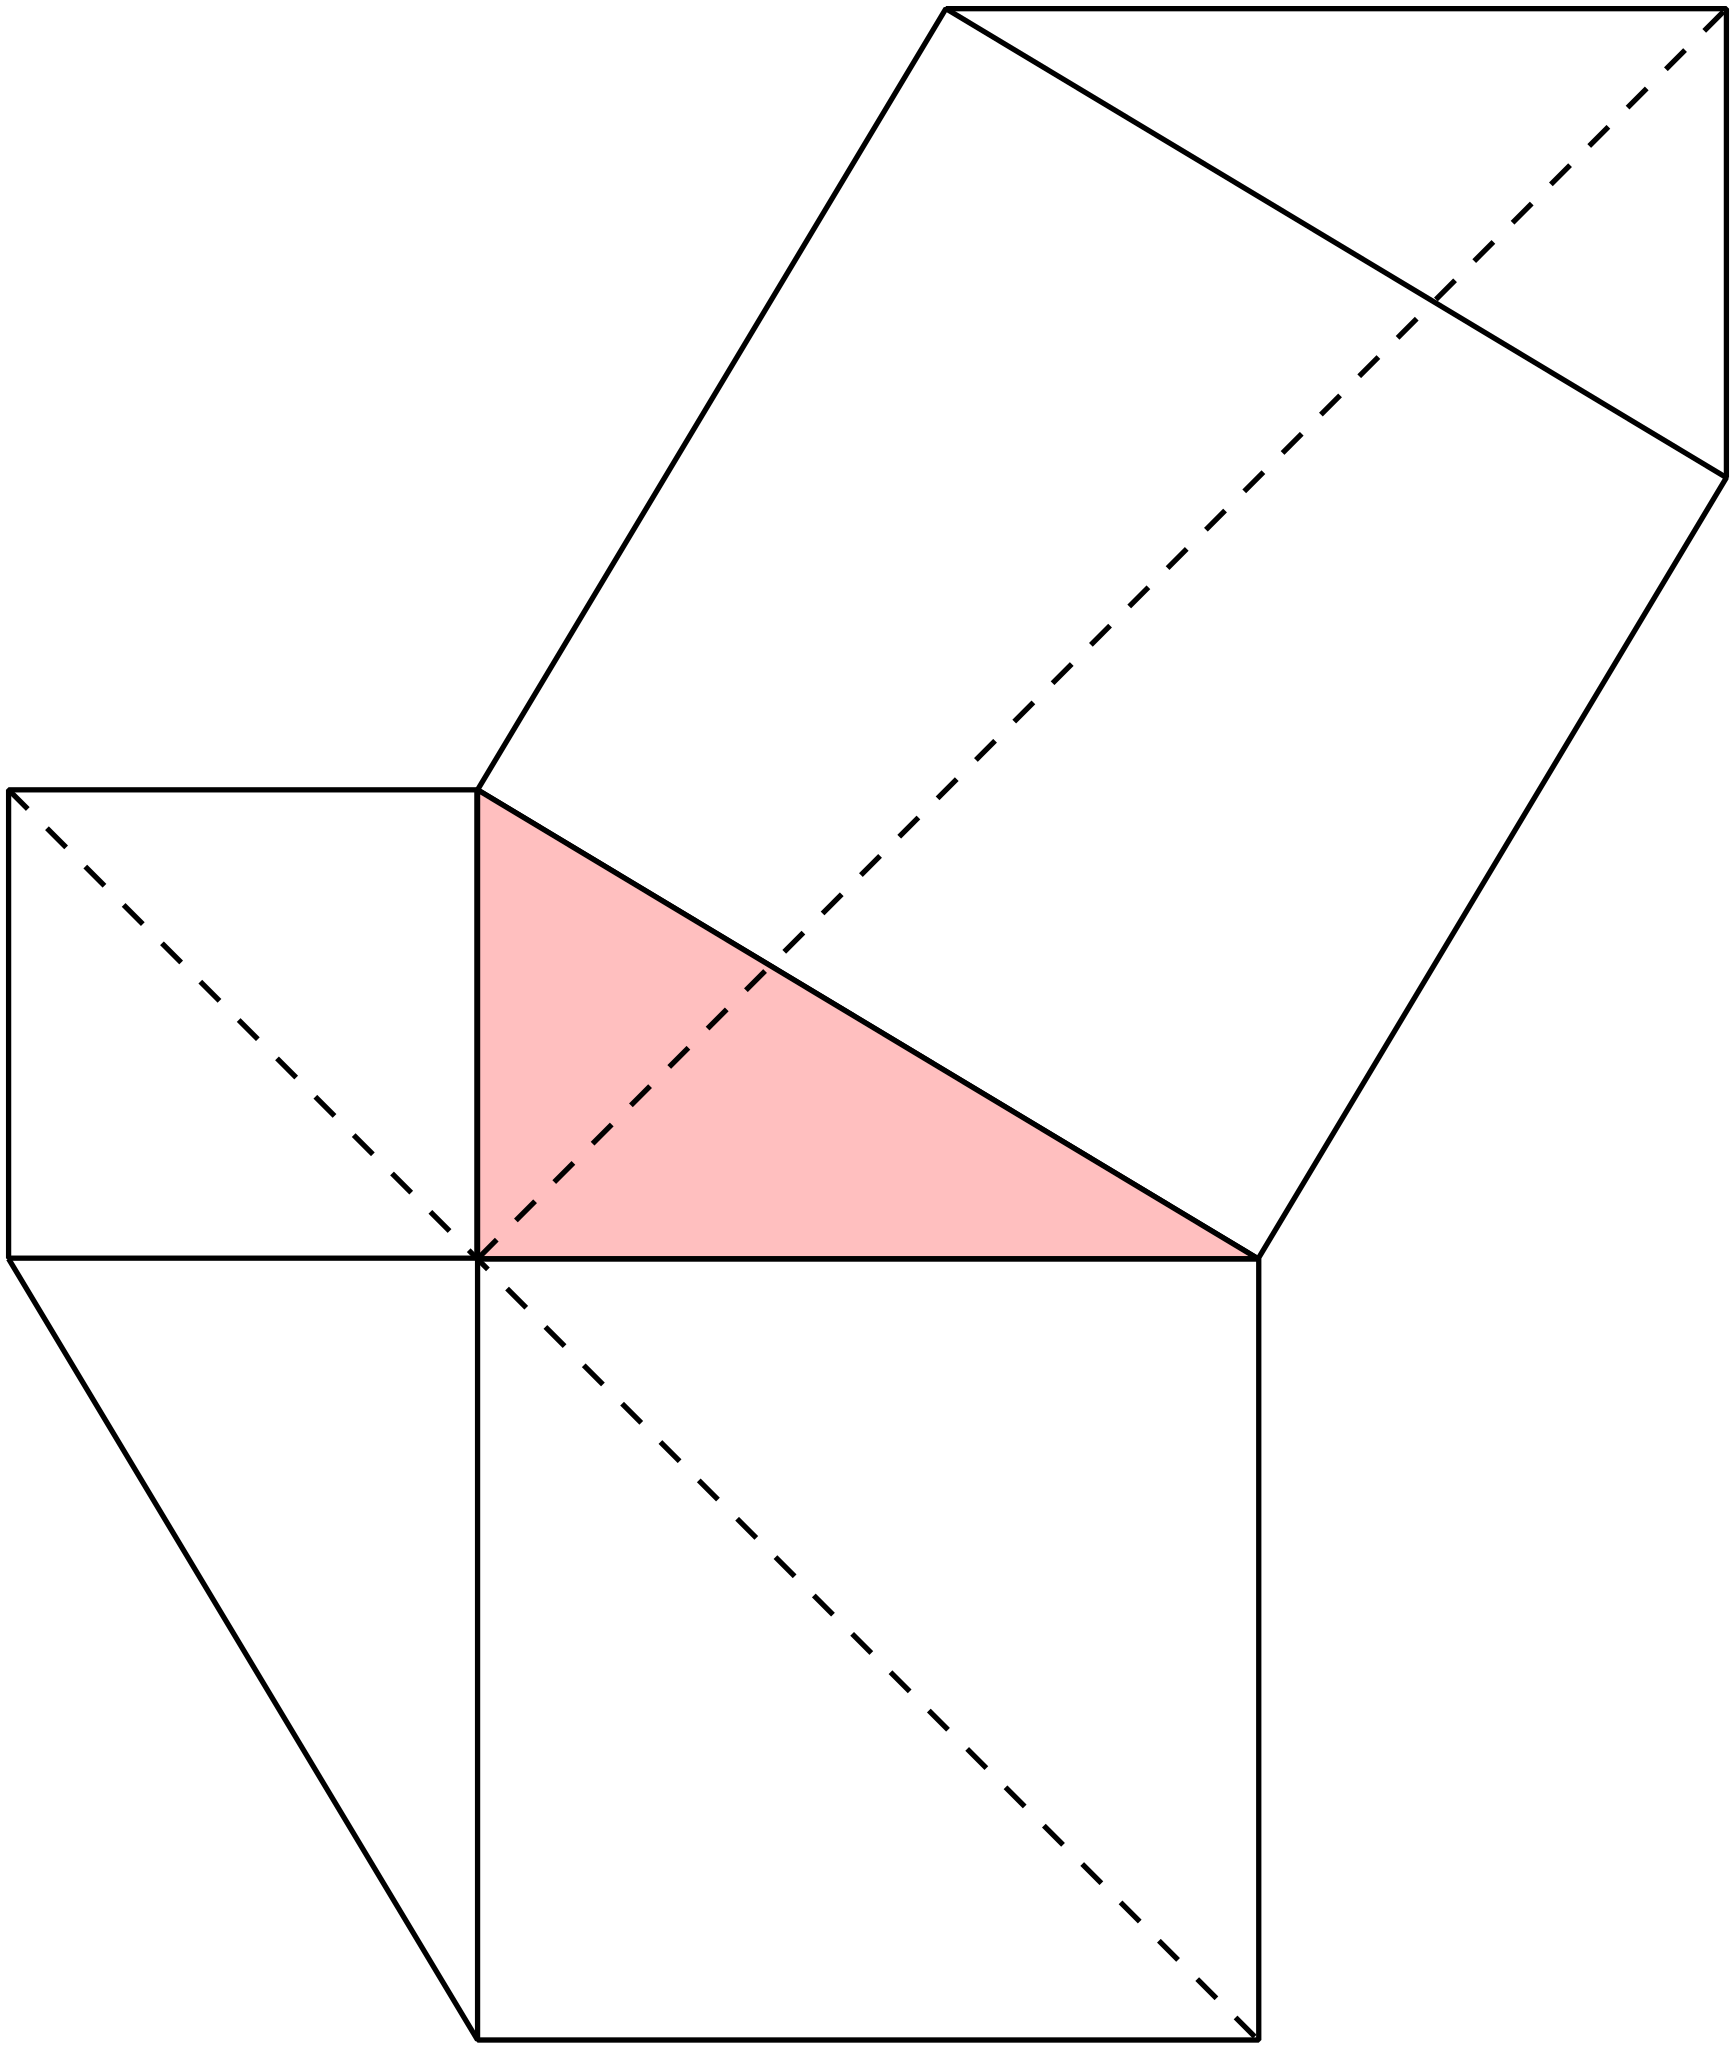
\includegraphics{../graphics/pbpdavinci.pdf}
\]
Note: This proof is due to Leonardo da Vinci.
%\item Explain how the following picture ``proves'' the Pythagorean Theorem.
%\[
%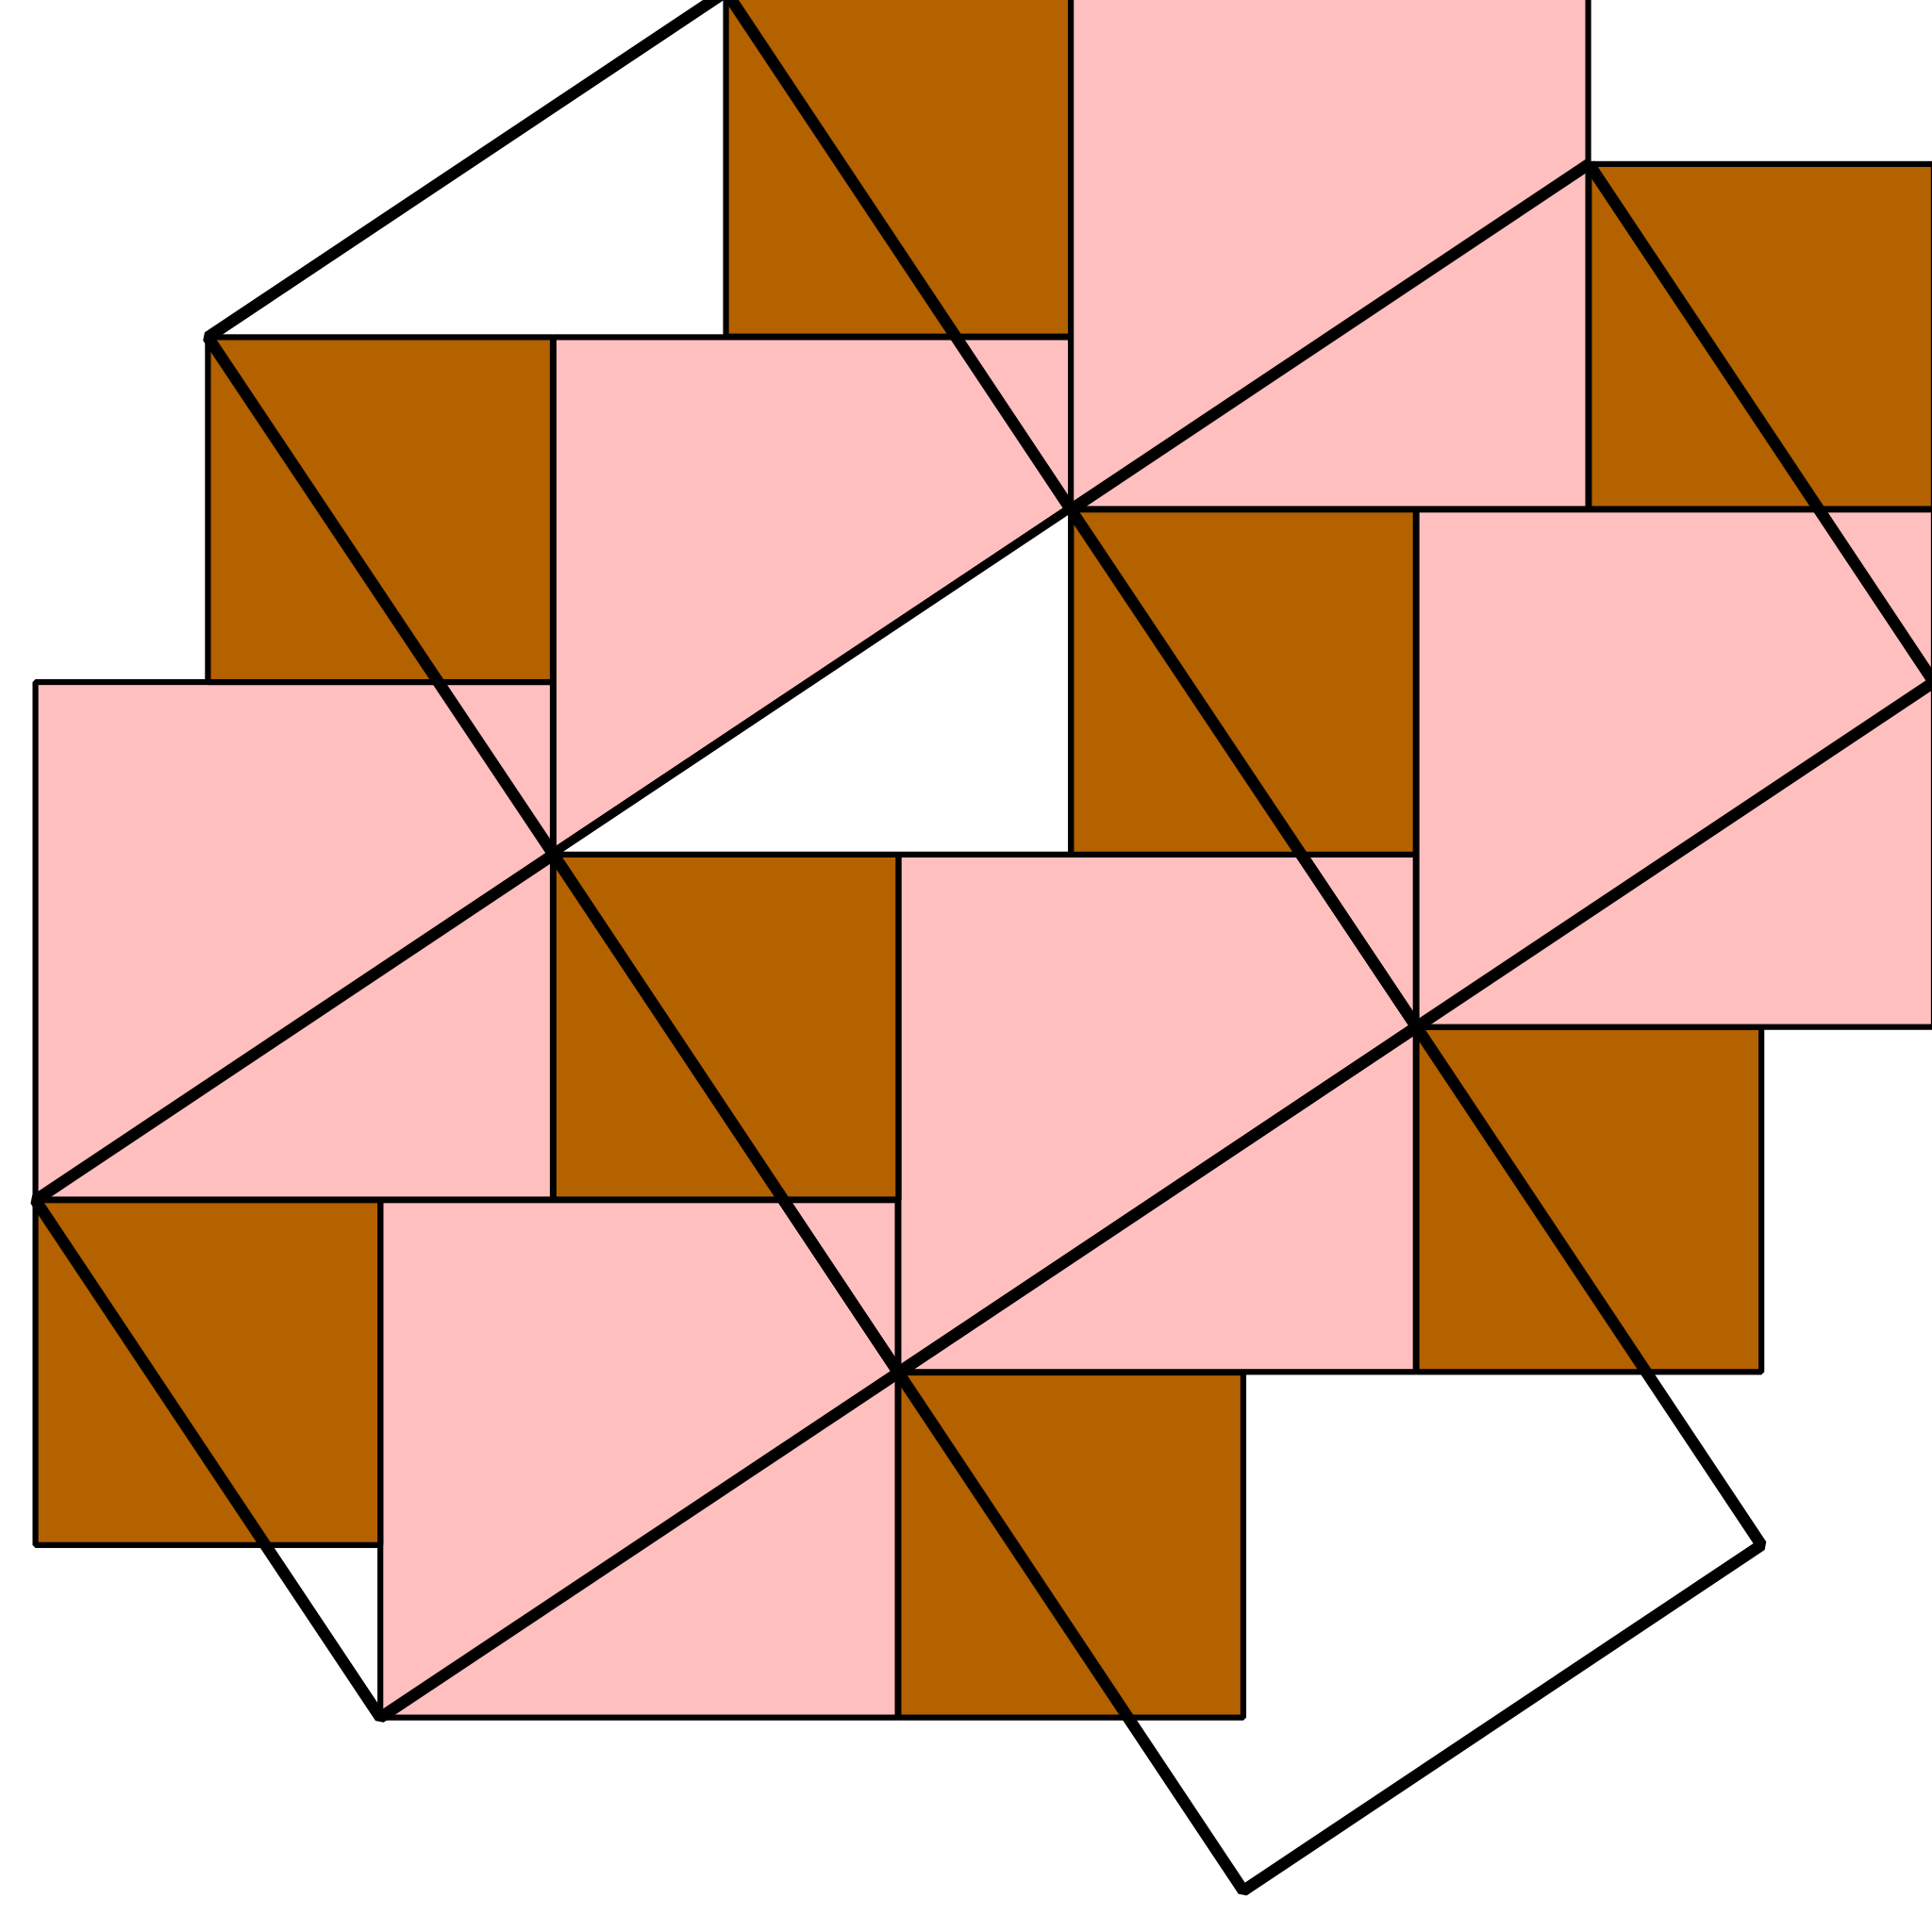
\includegraphics{../graphics/pbppyth2.pdf}
%\]
%\item Use the following tessellation to give a dissection proof of the Pythagorean Theorem.
%\[
%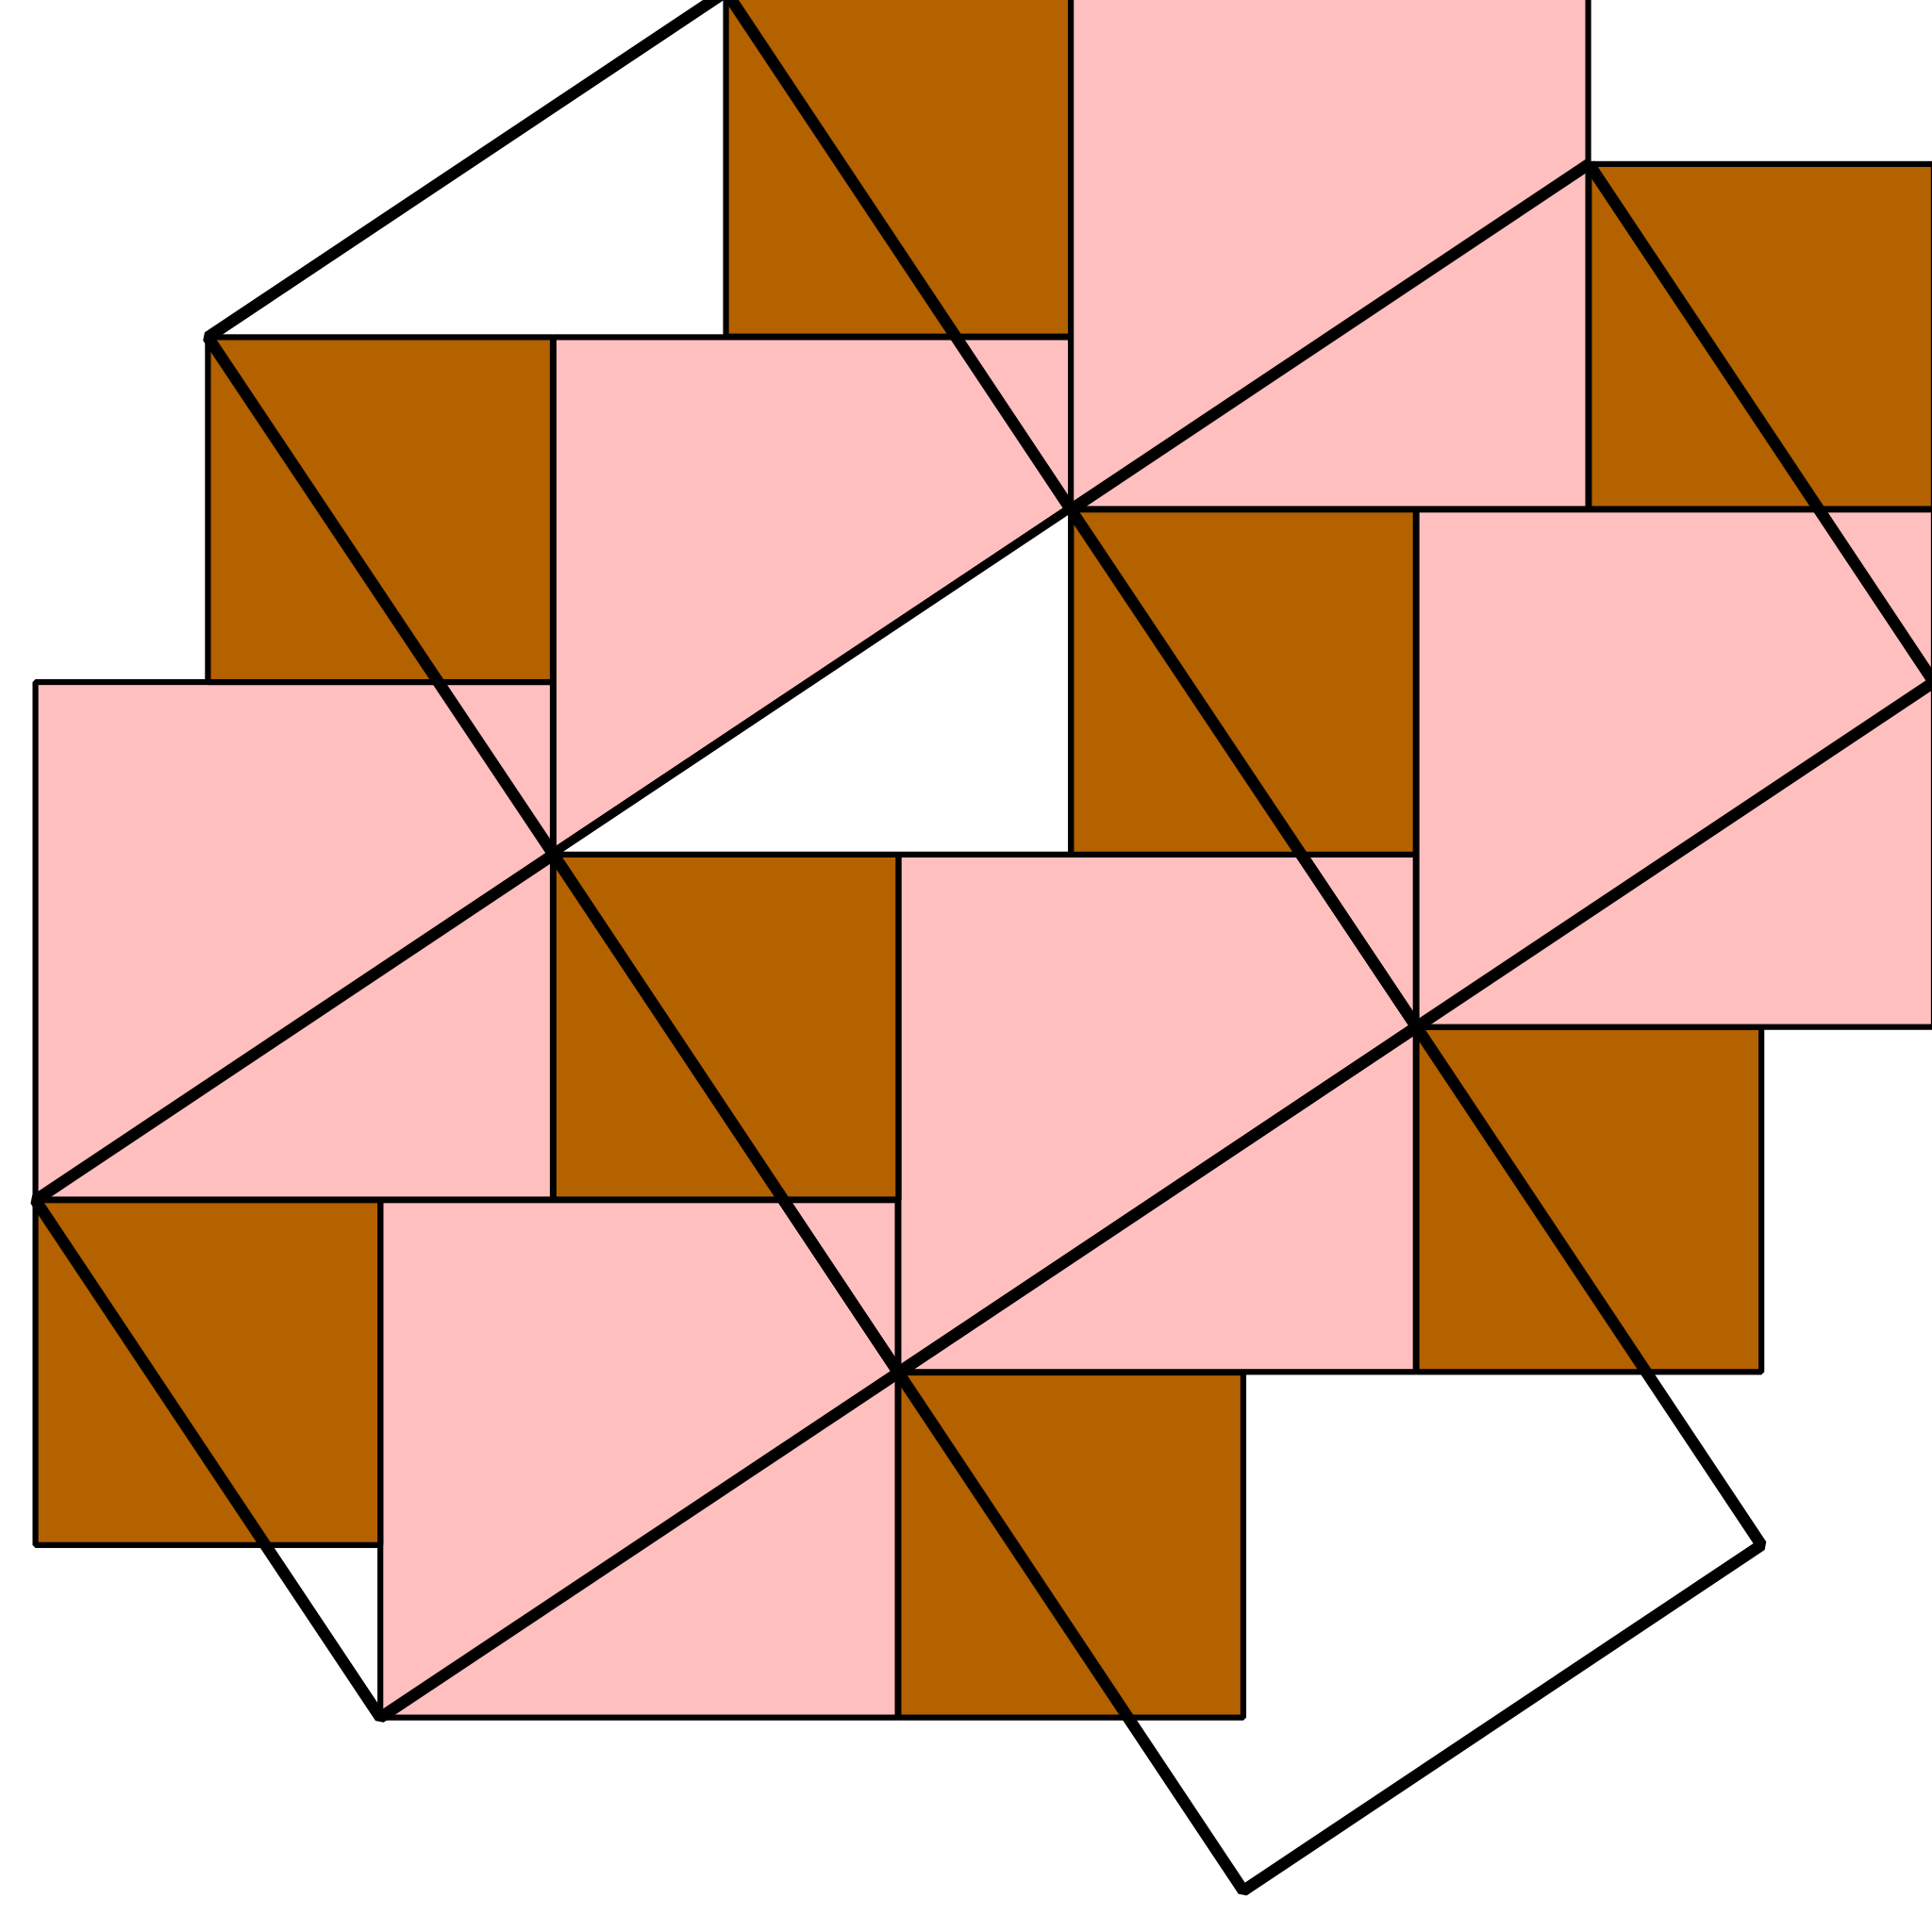
\includegraphics{../graphics/pbppyth2.pdf}
%\]
%\item Explain how the following picture ``proves'' the Pythagorean Theorem.
%\[
%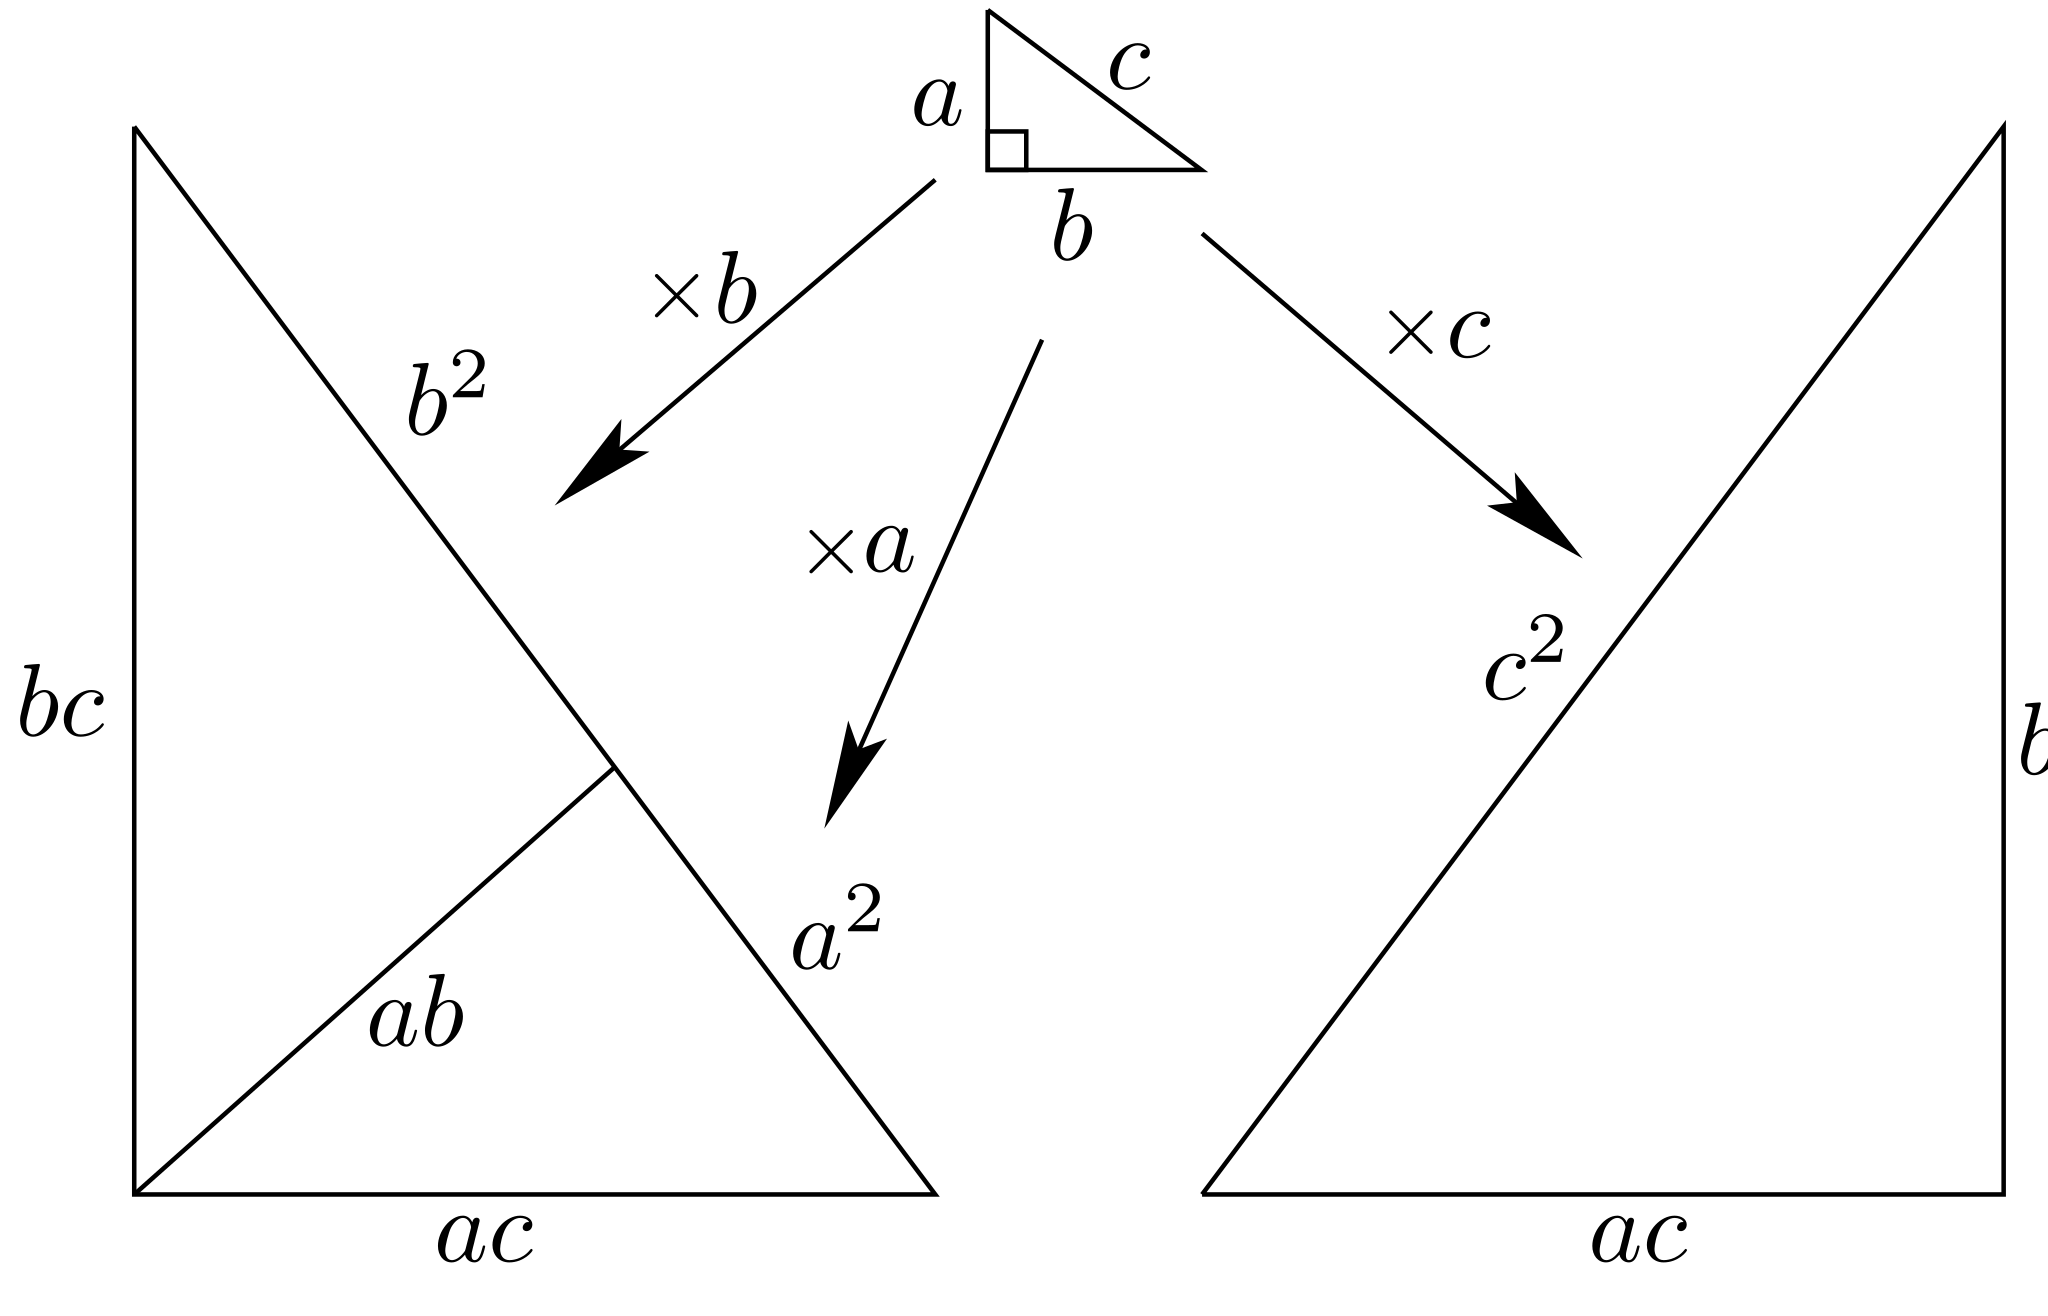
\includegraphics{../graphics/pbpdilation.pdf}
%\]
\item\label{P:pbptrap} Recall that a trapezoid is a quadrilateral with two parallel sides. Consider the following picture:
\[
\includegraphics{../graphics/trap.pdf}
\]
How does the above picture prove that the area of a trapezoid is
\[
\mathrm{area}= \frac{h(b_1 + b_2)}{2},
\]
where $h$ is the height of the trapezoid and $b_1$, $b_2$, are the lengths of the parallel sides?
\item Explain how the following picture ``proves'' the Pythagorean Theorem.
\[
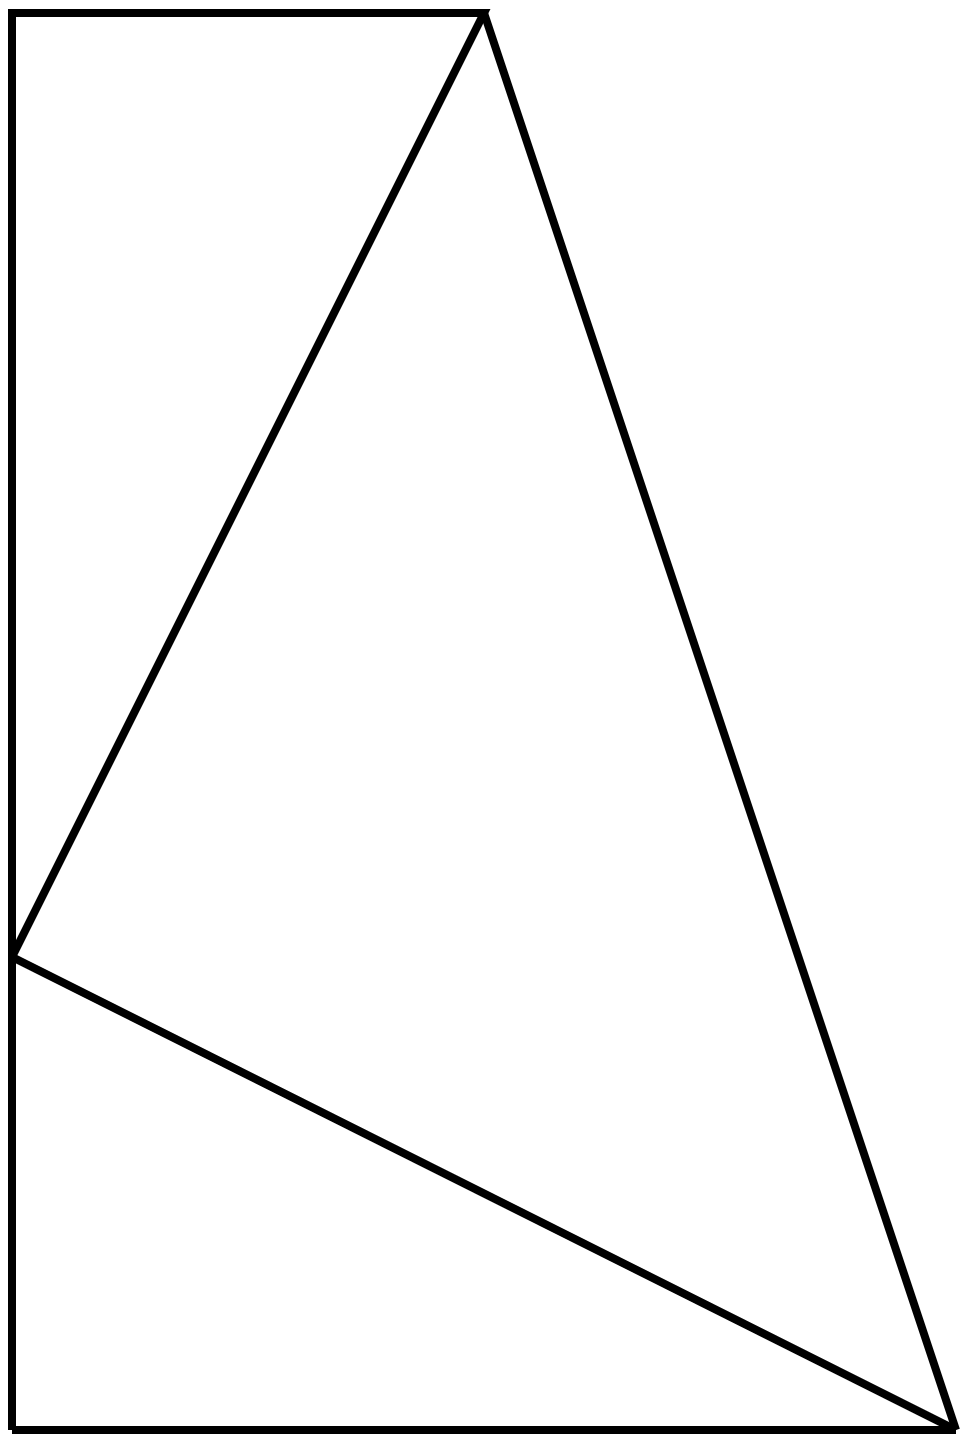
\includegraphics{../graphics/pbptrap.pdf}
\]
Note: This proof is due to James A.\ Garfield, the 20th President of the United States.
\item Look at Problem~\ref{P:pbptrap}. Can you use a similar picture
  to prove that the area of a parallelogram
\[
\includegraphics{../graphics/para.pdf}
\]
is the length of the base times the height?
\item Explain how the following picture ``proves'' that the area of a
  parallelogram is base times height.
\[
\includegraphics{../graphics/para3.pdf}
\]
Now suppose that a student, say \textit{Geometry Giorgio} attempts to
solve a similar problem. In an attempt to prove the formula for the
area of a parallelogram, \textit{Geometry Giorgio} draws the following
picture:
\[
\includegraphics{../graphics/paragiorgio.pdf}
\]
At this point \textit{Geometry Giorgio} says that he has proved the
formula for area of a parallelogram. What do you think of his picture?
Give a complete argument based on his picture.

\item Which of the above ``proofs'' for the formula for the area of a
  parallelogram is your favorite? Explain why.

\item Explain how the following picture ``proves'' that the area of a
  quadrilateral is equal to half of the area of the parallelogram
  whose sides are parallel to and equal in length to the diagonals of
  the original quadrilateral.
\[
\includegraphics[scale=.7]{../graphics/pbpquadarea.pdf}
\]

\item Explain how the following picture ``proves'' that if a
  quadrilateral has two opposite angles that are equal, then the
  bisectors of the other two angles are parallel or on top of each
  other.
\[
\includegraphics[scale=.7]{../graphics/119hw5_2.pdf}
\]



\break

\item\label{P:Tparadox1} Why might someone find the following picture
  disturbing? How would you assure them that actually everything is
  good and well in the geometrical world?
\[
\includegraphics[scale=.8]{../graphics/triparadox.pdf}
\]



\item\label{P:Tparadox2} Why might someone find the following picture
  disturbing? How would you assure them that actually everything is
  good and well in the geometrical world?
\[
\includegraphics[scale=.8]{../graphics/triparadox2.pdf}
\]


\item How could you explain to someone that doubling the lengths of each side of a cube does not double the volume of the cube?

\item\label{P:sq1}  Explain how the following picture ``proves'' that:
\[
\frac{1}{2} + \left(\frac{1}{2}\right)^2 +  \left(\frac{1}{2}\right)^3 +  \left(\frac{1}{2}\right)^4 +  \left(\frac{1}{2}\right)^5 + \cdots = 1
\]
\[
\includegraphics{../graphics/pbpsqgeo.pdf}
\]
\item\label{P:sq2}  Explain how the following picture ``proves'' that if $0 < r < 1$:
\[
r + r(1-r) + r(1-r)^2 + r(1-r)^3 + \cdots = 1
\]
\[
\includegraphics{../graphics/pbpgengeo.pdf}
\]
\item\label{P:tri1} Explain how the following picture ``proves'' that:
\[
\frac{1}{4} + \left(\frac{1}{4}\right)^2 +  \left(\frac{1}{4}\right)^3 +  \left(\frac{1}{4}\right)^4 +  \left(\frac{1}{4}\right)^5 + \cdots = \frac{1}{3}
\]
\[
\includegraphics{../graphics/pbptriangle.pdf}
\]
\item Considering Problem~\ref{P:sq1}, Problem~\ref{P:sq2}, and
  Problem~\ref{P:tri1} can you give a new picture ``proving'' that: 
\[
\frac{1}{4} + \left(\frac{1}{4}\right)^2 +  \left(\frac{1}{4}\right)^3 +  \left(\frac{1}{4}\right)^4 +  \left(\frac{1}{4}\right)^5 + \cdots = \frac{1}{3}
\]
Carefully explain the connection between your picture and the
mathematical expression above.

\item Explain how the following picture ``proves'' that  in any packing, the number of calissons with a given orientation is exactly one-third the total number of calissons in the box.
\[
\includegraphics{../graphics/pbpcas.pdf}
\]
\end{enumerate}
\end{problems}


\chapter{Compass and Straightedge Constructions}
\begin{quote} 
\begin{tabular}{rl}
\textit{Mephistopheles:} & I must say there is an obstacle \\
                         & That prevents my leaving:\\
                         & It's the pentagram on your threshold.\\
\textit{Faust:}          & The pentagram impedes you? \\
                         & Tell me then, you son of hell,\\
                         & If this stops you, how did you come in?\\
\textit{Mephistopheles:} & Observe! The lines are poorly drawn;\\
                         & That one, the outer angle, \\
                         & Is open, the lines don't meet.
\end{tabular}

\hfill---G\"othe, \textit{Faust} act I, scene III
\end{quote}

\section{Constructions}

About a century before the time of \index{Euclid}Euclid,
\index{Plato}Plato---a student of \index{Socrates}Socrates---declared
that the compass and straightedge should be the only tools of the
geometer. Why would he do such a thing? For one thing, both the the
compass and straightedge are fairly simple instruments. One draws
circles, the other draws lines---what else could possibly be needed to
study geometry? Moreover, rulers and protractors are far more complex
in comparison and people back then couldn't just walk to the campus
bookstore and buy whatever they wanted. However, there are other
reasons:
\begin{enumerate}        
\item Compass and straightedge constructions are \textbf{independent
  of units}.
\item Compass and straightedge constructions are \textbf{theoretically
  correct}.
\item Combined, the compass and straightedge seem like
  \textbf{powerful tools}.
\end{enumerate}



\paragraph{Compass and straightedge constructions are \textbf{independent of units}.} 
Whether you are working in centimeters or miles, compass and
straightedge constructions work just as well. By not being locked to
set of units, the constructions given by a compass and straightedge
have certain generality that is appreciated even today.


\paragraph{Compass and straightedge constructions are \textbf{theoretically correct}.} 
In mathematics, a correct method to solve a problem is more valuable
than a correct solution. In this sense, the compass and straightedge
are ideal tools for the mathematician. Easy enough to use that the
rough drawings that they produce can be somewhat relied upon, yet
simple enough that the tools themselves can be described
theoretically. Hence it is usually not too difficult to connect a
given construction to a formal proof showing that the construction is
correct.


\paragraph{Combined, the compass and straightedge seem like \textbf{powerful tools}.} 
No tool is useful unless it can solve a lot of problems. Without a
doubt, the compass and straightedge combined form a powerful
tool. Using a compass and straightedge, we are able to solve many
problems exactly. Of the problems that we cannot solve exactly, we can
always produce an approximate solution.





\index{constructions|see{compass and straightedge \textit{or}
    origami}} We'll start by giving the rules of compass and
straightedge constructions:

\subsubsection*{Rules for Compass and Straightedge Constructions}
\begin{enumerate}
\item You may only use a compass and straightedge.
\item You must have two points to draw a line.
\item You must have a point and a line segment to draw a circle. The
  point is the center and the line segment gives the radius.
\item Points can only be placed in two ways:
\begin{enumerate}
\item As the intersection of lines and/or circles.
\item As a \textbf{free point}\index{free point}, meaning the location
  of the point is not important for the final outcome of the
  construction.
\end{enumerate}
\end{enumerate}

Our first construction is also Euclid's first construction:

\begin{construction}[Equilateral Triangle]\index{compass and straightedge!equilateral triangle} We wish to construct an equilateral triangle given the length of one 
side.
\begin{enumerate} 
\item Open your compass to the width of the line segment.
\item Draw two circles, one with the center being each end point 
of the line segment.
\item The two circles intersect at two points.  Choose one and 
connect it to both of the line segment's endpoints.
\end{enumerate}
\[
\includegraphics{../graphics/eqtri.pdf}
\]
\end{construction}

Euclid's second construction will also be our second construction:

\begin{construction}[Transferring a Segment]\index{compass and straightedge!transferring a segment}
Given a segment, we wish to move it so that it starts on a given
point, on a given line.
\begin{enumerate}        
\item Draw a line through the point in question.
\item Open your compass to the length of the line segment and draw a circle with the given point as its center.
\item The line segment consisting of the given point and the intersection of the circle and the line 
is the transferred segment.
\end{enumerate}
\end{construction}

If you read \emph{The Elements}, you'll see that Euclid's construction is
much more complicated than ours.   Apparently, Euclid felt the need to
justify the ability to move a distance. Many sources say that Euclid
used what is called a \index{compass!collapsing}\index{collapsing
compass}\textit{collapsing compass}, that is a compass that collapsed
when it was picked up. However, I do not believe that such an
invention ever existed. Rather this is something that lives in the
conservative geometer's head.


Regardless of whether the difficulty of transferring distances was theoretical
or physical, we need not worry when we do it.  In fact, Euclid's
proof of the above theorem proves that our modern way of using the
compass to transfer distances is equivalent to using the so-called
collapsing compass.

\begin{question} Exactly how would one prove that the modern compass is equivalent 
to the collapsing compass? Hint: See Euclid's proof.
\end{question}
\QM


\begin{construction}[Bisecting a Segment]\index{compass and straightedge!bisecting a segment} 
Given a segment, we wish to cut it in half.
\begin{enumerate}
\item Open your compass to the width of the segment.
\item Draw two circles, one with the center being at each end point 
of the line segment.
\item The circles intersect at two points.  Draw a line through 
these two points.
\item The new line bisects the original line segment.
\end{enumerate}
\[
\includegraphics{../graphics/bisectseg.pdf}
\]
\end{construction}

\begin{construction}[Perpendicular to a Line through a Point]\index{compass and straightedge!perpendicular to a line through a point}  
Given a point and a line, we wish to construct a line perpendicular to
the original line that passes through the given point.
\begin{enumerate}
\item Draw a circle centered at the point large enough  
       to intersect the line in two distinct points.
\item Bisect the line segment. The line used to do this 
       will be the desired line.
\end{enumerate}
\[
\includegraphics{../graphics/perpfrompoint.pdf}
\]
\end{construction}





\begin{construction}[Bisecting an Angle]\index{compass and straightedge!bisecting an angle} 
We wish to divide an angle in half.
\begin{enumerate}
\item Draw a circle with its center being the vertex of the 
angle.
\item Draw a line segment where the circle intersects the lines.
\item Bisect the new line segment.  The bisector will bisect the angle.
\end{enumerate}
\[
\includegraphics{../graphics/bisectangle.pdf}
\]
\end{construction}


We now come to a very important construction:

\begin{construction}[Copying an Angle]\index{compass and straightedge!copying an angle} 
Given a point on a line and some angle, we wish to copy the 
given angle so that the new angle has the point as its 
vertex and the line as one of its edges.
\begin{enumerate}
\item Open the compass to a fixed width and make a circle 
centered at the vertex of the angle.
\item Make a circle of the same radius on the line with the point.
\item Open the compass so that one end touches the $1$st circle 
where it hits an edge of the original angle, with the other end of the compass extended to where the $1$st circle hits the other edge of the original angle.
\item Draw a circle with the radius found above with its center 
where the second circle hits the line.
\item Connect the point to where the circles meet. This is the other leg of the angle we are constructing.
\end{enumerate}
\[
\includegraphics{../graphics/copyangle.pdf}
\]
\end{construction}



\begin{construction}[Parallel to a Line through a Point]\index{compass and straightedge!parallel to a line through a point} 
 Given a line and a point, we wish to construct another line parallel
 to the first that passes through the given point.
\begin{enumerate}
\item Draw a circle around the given point that passes through the given line at two points.
\item We now have an isosceles triangle, duplicate this triangle.
\item Connect the top vertexes of the triangles and we get a parallel line.
\end{enumerate}
\vspace{1cm}
\[
\includegraphics{../graphics/parallel.pdf}
\]
\end{construction}


\begin{question} Can you give another different construction?
\end{question}
\QM


\begin{problems}
\begin{enumerate}
\item What are the rules for compass and straightedge constructions?
\item What is a collapsing compass? Why don't we use them or worry about them any more?
\item Prove that the collapsing compass is equivalent to the modern compass.
\item Given a line segment, construct an equilateral triangle whose edge has the length of the given segment. Explain the steps in your construction.
\item Use a compass and straightedge to bisect a given line segment. Explain the steps in your construction.
\item Given a line segment with a point on it, construct a line perpendicular to the segment that passes through the given point. Explain the steps in your construction.
\item Use a compass and straightedge to bisect a given angle. Explain the steps in your construction.
\item Given an angle and some point, use a compass and straightedge to copy the angle so that the new angle has as its vertex the given point. Explain the steps in your construction.
\item Given a point and line, construct a line perpendicular to the given line that passes through the given point. Explain the steps in your construction.
\item Given a point and line, construct a line parallel to the given line that passes through the given point. Explain the steps in your construction.
\item Given a length of $1$, construct a triangle whose perimeter is a
  multiple of $6$. Explain the steps in your construction.
\item Construct a $30$-$60$-$90$ right triangle. Explain the steps in your
  construction.
\item Given a length of $1$, construct a triangle with a perimeter of
  $3 + \sqrt{5}$. Explain the steps in your construction.
\item Given a length of $1$, construct a triangle with a perimeter that is a multiple of
  $2 + \sqrt{2}$. Explain the steps in your construction.
\item Here is a circle and here is the side length of an inscribed
  regular $5$-gon.
\[
\includegraphics{../graphics/5gonPiece.pdf}
\]
Construct the regular $5$-gon. Explain the steps in your construction.
\item Here is a piece of a regular $7$-gon.
\[
\includegraphics{../graphics/7gonPiece.pdf}
\]
Construct the entire regular $7$-gon. Explain the steps in your
construction.
\end{enumerate}
\end{problems}

\newpage



\section{Anatomy of Figures}


In studying geometry we seek to discover the points that can be
obtained given a set of rules. In our case the set of rules consists
of the rules for compass and straightedge constructions.

\begin{question} 
In regards to compass and straightedge constructions, what is a
\textit{point}?
\end{question}
\QM

\begin{question}
In regards to compass and straightedge constructions, what is a
\textit{line}?
\end{question}
\QM


\begin{question}
In regards to compass and straightedge constructions, what is a
\textit{circle}?
\end{question}
\QM


OK, those are our basic figures, pretty easy right? Now I'm going to
quiz you about them:

\begin{question} 
Place two points randomly in the plane. Do you expect to be able to
draw a single line that connects them?
\end{question}
\QM

\begin{question} 
Place three points randomly in the plane. Do you expect to be able to
draw a single line that connects them?
\end{question}
\QM

\begin{question} 
Place two lines randomly in the plane. How many points do you expect
them to share?
\end{question}
\QM


\begin{question} 
Place three lines randomly in the plane. How many points do you expect
all three lines to share?
\end{question}
\QM


\begin{question} 
Place three points randomly in the plane. Will you (almost!) always be
able to draw a circle containing these points? If no, why not? If yes,
how do you know?
\end{question}
\QM




\subsection{Lines Related to Triangles}

Believe it or not, in mathematics we often try to study the simplest
objects as deeply as possible. After the objects listed above,
triangles are among the most basic of geometric figures, yet there is
much to know about them.  There are several lines that are commonly
associated to triangles. Here they are:
\begin{itemize}
\item Perpendicular bisectors of the sides.
\item Bisectors of the angles.
\item Altitudes of the triangle.
\item Medians of the triangle. 
\end{itemize}

The first two lines above are self-explanatory. The next two need definitions.

\begin{definition}\index{altitude} 
An \textbf{altitude} of a triangle is a line segment originating at a
vertex of the triangle that meets the line containing the opposite
side at a right angle.
\end{definition}


\begin{definition}\index{median} 
A \textbf{median} of a triangle is a line segment that connects a
vertex to the midpoint of the opposite side.
\end{definition}

\begin{question} 
The intersection of any two lines containing the altitudes of a
triangle is called an \textbf{orthocenter}\index{orthocenter}. How
many orthocenters does a given triangle have?
\end{question}
\QM


\begin{question} 
The intersection of any two medians of a triangle is called a
\textbf{centroid}\index{centroid}. How many centroids does a given
triangle have?
\end{question}
\QM


\begin{question} What is the physical meaning of a centroid?
\end{question}
\QM




\subsection{Circles Related to Triangles}


There are also two circles that are commonly associated to
triangles. Here they are:
\begin{itemize}
\item The circumcircle.
\item The incircle.
\end{itemize}

These aren't too bad. Check out the definitions.

\begin{definition}\index{circumcircle}\index{circumcenter}
The \textbf{circumcircle} of a triangle is the circle that contains
all three vertexes of the triangle. Its center is called the
\textbf{circumcenter} of the triangle.
\[
\includegraphics[width=2in]{../graphics/circumcircle.pdf}
\]
\end{definition}

\begin{question} Does every triangle have a circumcircle?
\end{question}
\QM

\begin{definition}\index{incircle}\index{incenter}
The \textbf{incircle} of a triangle is the largest circle that will
fit inside the triangle. Its center is called the \textbf{incenter} of
the triangle.
\[
\includegraphics[width=2in]{../graphics/incircle.pdf}
\]
\end{definition}


\begin{question} Does every triangle have an incircle?
\end{question}
\QM


\begin{question} 
Are any of the lines described above related to these circles and/or
centers? Clearly articulate your thoughts.
\end{question}
\QM


\begin{problems}
\begin{enumerate}
\item Compare and contrast the idea of ``intersecting sets'' with the
  idea of ``intersecting lines.''
\item Place three points in the plane. Give a detailed discussion
  explaining how they may or may not be on a line.
\item Place three lines in the plane. Give a detailed discussion explaining
  how they may or may not intersect.
\item Explain how a perpendicular bisector is different from an
  altitude. Draw an example to illustrate the difference.
\item Explain how a median is different from an angle bisector.  Draw an
  example to illustrate the difference.
\item What is the name of the point that is the same distance from all
  three sides of a triangle? Explain your reasoning.
\item What is the name of the point that is the same distance from all
  three vertexes of a triangle? Explain your reasoning.
\item Could the circumcenter be outside the triangle? If so, draw a
  picture and explain. If not, explain why not using pictures as
  necessary.
\item Could the orthocenter be outside the triangle? If so, draw a
  picture and explain. If not, explain why not using pictures as
  necessary.
\item Could the incenter be outside the triangle? If so, draw a
  picture and explain. If not, explain why not using pictures as
  necessary.
\item Could the centroid be outside the triangle? If so, draw a
  picture and explain. If not, explain why not using pictures as
  necessary.
\item Are there shapes that do not contain their centroid? If so, draw
  a picture and explain. If not, explain why not using pictures as
  necessary.
\item Draw an equilateral triangle. Now draw the lines containing the
  altitudes of this triangle. How many orthocenters do you have as
  intersections of lines in your drawing? Hints:
\begin{enumerate}
\item More than one.
\item How many triangles are in the picture you drew?
\end{enumerate}
\item Given a triangle, construct the circumcenter. Explain the steps
  in your construction.\index{circumcenter}
\item Given a triangle, construct the orthocenter. Explain the steps
  in your construction.\index{orthocenter}
\item Given a triangle, construct the incenter. Explain the steps in
  your construction.\index{incenter}
\item Given a triangle, construct the centroid. Explain the steps in
  your construction.\index{centroid}
\item Given a triangle, construct the incircle. Explain the steps in
  your construction.\index{incircle}
\item Given a triangle, construct the circumcircle. Explain the steps
  in your construction.\index{circumcircle}
\item Given a circle, give a construction that finds its center. 
\item Where is the circumcenter of a right triangle? Explain your
  reasoning.
\item Where is the orthocenter of a right triangle? Explain your
  reasoning.
\item Can you draw a triangle where the circumcenter, orthocenter,
  incenter, and centroid are all the same point?  If so, draw a
  picture and explain. If not, explain why not using pictures as
  necessary.
\item True or False: Explain your conclusions.
\begin{enumerate}
\item An altitude of a triangle is always perpendicular to a line
  containing some side of the triangle.
\item An altitude of a triangle always bisects some side of the
  triangle.
\item The incenter is always inside the triangle.
\item The circumcenter, the centroid, and the orthocenter always lie in a line.
\item The circumcenter can be outside the triangle.
\item The orthocenter is always inside the triangle.
\item The centroid is always inside the incircle.
\end{enumerate}
\item Given 3 distinct points not all in a line, construct a circle
  that passes through all three points. Explain the steps in your
  construction.
\end{enumerate}
\end{problems}

\newpage

\section{Trickier Constructions}

\begin{question} 
How do you construct regular polygons? In particular, how do you
construct regular: $3$-gons, $4$-gons, $5$-gons, $6$-gons, $7$-gons,
$8$-gons, $10$-gons, $12$-gons, $17$-gons, $24$-gons, and $144$-gons?
\end{question}
\QM

Well the equilateral triangle is easy. It was the first construction
that we did. What about squares? What about regular hexagons? It turns
out that they aren't too difficult. What about pentagons? Or say
$n$-gons? We'll have to think about that. Let's leave the difficult
land of $n$-gons and go back to thinking about nice, three-sided
triangles.

\begin{construction}[SAS Triangle]\index{compass and straightedge!SAS triangle}  
Given two sides with an angle between them, we wish to construct the
triangle with that angle and two adjacent sides.
\begin{enumerate}
\item Transfer the one side so that it starts at the vertex of the
  angle.
\item Transfer the other side so that it starts at the vertex. 
\item Connect the end points of all moved line segments.
\end{enumerate}
\end{construction}

The ``SAS'' in this construction's name spawns from the fact that it
requires two sides with an angle \textit{between} them. The SAS
Theorem states that we can obtain a unique triangle given two sides
and the angle between them.


\begin{construction}[SSS Triangle]\index{compass and straightedge!SSS triangle} 
Given three line segments we wish to construct the triangle that has
those three sides if it exists.
\begin{enumerate}
\item Choose a side and select one of its endpoints.
\item Draw a circle of radius equal to the length of the second side
  around the chosen endpoint.
\item Draw a circle of radius equal to the length of the third side
  around the other endpoint.
\item Connect the end points of the first side and the intersection of
  the circles. This is the desired triangle.
\end{enumerate}
\end{construction}


\begin{question} 
Can this construction fail to produce a triangle? If so, show how. If
not, why not?
\end{question}
\QM

\begin{question}
Remember earlier when we asked about the converse to the Pythagorean
Theorem?\index{Pythagorean Theorem} Can you use the construction above
to prove the converse of the Pythagorean Theorem?
\end{question}
\QM

\begin{question}
Can you state the SSS Theorem?
\end{question}
\QM


\begin{construction}[SAA Triangle]\index{compass and straightedge!SAA triangle} 
Given a side and two angles, where the given side does not touch one
of the angles, we wish to construct the triangle that has this side
and these angles if it exists.
\begin{enumerate}
\item Start with the given side and place the adjacent angle at one of
  its endpoints.
\item Move the second angle so that it shares a leg with the leg of
  the first angle--not the leg with the side.
\item Extend the side past the first angle, forming a new angle with
  the leg of the second angle.
\item Move this new angle to the other endpoint of the side, extending
  the legs of this angle and the first angle will produce the desired
  triangle.
\end{enumerate}
\end{construction}


\begin{question} 
Can this construction fail to produce a triangle? If so, show how. If
not, why not?
\end{question}
\QM

\begin{question}
Can you state the SAA Theorem?
\end{question}
\QM

\begin{question} What about other combinations of S's and A's?
\[
\text{SSS},\quad \text{SSA},\quad \text{SAS},\quad \text{SAA},\quad \text{ASA},\quad \text{AAA} 
\]
\end{question}
\QM

\subsection{Challenge Constructions}

\begin{question} 
How can you construct a triangle given the length of one side $s$, the
length of the median to that side $m$, and the length of the
altitude of the opposite angle $a$?
\end{question}

\begin{proof}[Follow-Along] 
Use these lengths and follow the directions below.
\[
\includegraphics{../graphics/challenge1.pdf}
\]
\begin{enumerate}
\item Start with the given side.
\item Since the median hits our side at the center, bisect the given
  side.
\item Make a circle of radius equal to the length of the median
  centered at the bisector of the given side.
\item Construct a line parallel to our given line of distance equal to
  the length of the given altitude away.
\item Where the line and the circle intersect is the third point of
  our triangle. Connect the endpoints of the given side and the new
  point to get the triangle we want.
\end{enumerate}
\end{proof}


\begin{question} How can you construct a triangle given one angle $\alpha$, the 
length of an adjacent side $s$, and the altitude to that side $a$?
\end{question}

\begin{proof}[Follow-Along]
Use these and follow the directions below.
\[
\includegraphics{../graphics/challenge2.pdf}
\]
\begin{enumerate}
\item Start with a line containing the side.
\item Put the angle at the end of the side.
\item Draw a parallel line to the side of the length of the altitude
  away.
\item Connect the angle to the parallel side. This is the third
  vertex. Connect the endpoints of the given side and the new point to
  get the triangle we want.
\end{enumerate}
\end{proof}


\begin{question} How can you construct a circle with a given radius tangent 
to two other circles?
\end{question}

\begin{proof}[Follow-Along]
Use these and follow the directions below.
\[
\includegraphics{../graphics/challenge3.pdf}
\]
\begin{enumerate}
\item Let $r$ be the given radius, and let $r_1$ and $r_2$ be the
  radii of the given circles.
\item Draw a circle of radius $r_1 + r$ around the center of the
  circle of radius $r_1$.
\item Draw a circle of radius $r_2 + r$ around the center of the
  circle of radius $r_2$.
\item Where the two circles drawn above intersect is the center of the
  desired circle.
\end{enumerate}
\end{proof}


\begin{question} 
Place two tacks in a wall. Insert a sheet of paper so that the edges
hit the tacks and the corner passes through the imaginary line between
the tacks. Mark where the corner of the piece of paper touches the
wall. Repeat this process, sliding the paper around. What curve do you
end up drawing?
\end{question}
\QM

\begin{question} How can you construct a triangle given an angle and the 
length of the opposite side?
\end{question}

\begin{proof}[Solution] 
We really can't solve this problem completely because the information
given doesn't uniquely determine a triangle. However, we can still say
something. Here is what we can do:
\begin{enumerate}
\item Put the known angle at one end of the line segment. Note in the
  picture below, it is at the left end of the line segment and it is
  opening downwards.
\item Construct the perpendicular bisector of the given segment.
\item See where the bisector in Step 2 intersects the perpendicular of
  the other leg of the angle drawn from the vertex of the angle.
\item Draw arc centered at the point found in Step 3 that
  touches the endpoints of the original segment.
\end{enumerate}
\[
\includegraphics{../graphics/challenge4.pdf}
\]
Every point on the arc is a valid choice for the vertex of the
triangle.
\end{proof}

\begin{question} Why does the above method work?
\end{question}
\QM

\begin{question}\index{boat!lost at night} 
You are on a boat at night. You can see three lighthouses, and you
know their position on a map.  Also you know the angles of the light
rays between the lighthouses as measured from the boat.  How do you
figure out where you are?
\end{question}
\QM

\subsection{Problem Solving Strategies}

The harder constructions discussed in this section can be difficult to
do. There is no rote method to solve these problems, hence you must
rely on your brain. Here are some hints that you may find helpful:

\paragraph{Construct what you can.} 
You should start by constructing anything you can, even if you don't
see how it will help you with your final construction. In doing so you
are ``chipping away'' at the problem just as a rock-cutter chips away
at a large boulder. Here are some guidelines that may help when
constructing triangles:
\begin{enumerate}
\item If a side is given, then you should draw it.
\item If an angle is given and you know where to put it, draw it.
\item If an altitude of length $\l$ is given, then draw a line
  parallel to the side that the altitude is perpendicular to. This new
  line must be distance $\l$ from the side.
\item If a median is given, then bisect the segment it connects to and
  draw a circle centered around the bisector, whose radius is the
  length of the median.
\item If you are working on a figure, construct any ``mini-figures''
  inside the figure you are trying to construct. For example, many of
  the problems below ask you to construct a triangle. Some of these
  constructions have right-triangles inside of them, which are easier
  to construct than the final figure.
\end{enumerate}



\paragraph{Sketch what you are trying to find.} 
It is a good idea to try to sketch the figure that you are trying to
construct. Sketch it accurately and label all pertinent parts. If
there are special features in the figure, say two segments have the
same length or there is a right-angle, make a note of it on your
sketch. Also mark what is unknown in your sketch. We hope that doing
this will help organize your thoughts and get your ``brain juices''
flowing.\index{brain juices}

\begin{question} Why are the above strategies good?
\end{question}
\QM


\begin{problems}
\begin{enumerate}

%%% In Polya's book ``Mathematical Discovery'' he has some interesting
%%% notation for problems like the ones we give below. It may be good to
%%% use something like that in the future.

\item Construct a square. Explain the steps in your construction.

\item Construct a regular hexagon. Explain the steps in your construction.


\item Your friend Margy is building a clock. She needs to know how to align
the twelve numbers on her clock so that they are equally spaced on a
circle. Explain how to use a compass and straightedge construction to
help her out. Illustrate your answer with a construction and explain
the steps in your construction.

\item Construct a triangle given two sides of a triangle and the angle
  between them. Explain the steps in your construction.

\item State the SAS Theorem.

\item Construct a triangle given three sides of a triangle. Explain
  the steps in your construction.

\item State the SSS Theorem.


\item Construct a triangle given a side and two angles where one of
  the angles does not touch the given side. Explain the steps in your
  construction.

\item State the SAA Theorem.

\item Construct a triangle given a side between two given
  angles. Explain the steps in your construction.

\item State the ASA Theorem.

\item Explain why when given an isosceles triangle, that two
  of its angles have equal measure. Hint: Use the SAS Theorem.


\item Construct a figure showing that a triangle cannot always be
  uniquely determined when given an angle, a side adjacent to that
  angle, and the side opposite the angle. Explain the steps in your
  construction and explain how your figure shows what is
  desired. Explain what this says about the possibility of a SSA
  theorem.  Hint: Draw many pictures to help yourself out.

\item Give a construction showing that a triangle is uniquely
  determined if you are given a right-angle, a side touching that
  angle, and another side not touching the angle. Explain the steps in
  your construction and explain how your figure shows what is desired.

\item Construct a triangle given two adjacent sides of a triangle and
  a median to one of the given sides. Explain the steps in your
  construction.

\item Construct a triangle given two sides and the altitude to the
  third side. Explain the steps in your construction.

\item Construct a triangle given a side, the median to the side, and
  the angle opposite to the side. Explain the steps in your
  construction.

%\item Construct a triangle given two altitudes and an angle touching
%  one of them. Explain the steps in your construction. %% TANGENTS NEEDED


\item Construct a triangle given an altitude, and two angles not
  touching the altitude. Explain the steps in your construction.

\item Construct a triangle given the length of one side, the length of
  the the median to that side, and the length of the altitude of the
  opposite angle. Explain the steps in your construction.

\item Construct a triangle, given one angle, the length of an adjacent
  side and the altitude to that side. Explain the steps in your
  construction.

\item Construct a circle with a given radius tangent to two other
  given circles. Explain the steps in your construction.

\item Does a given angle and a given opposite side uniquely determine
  a triangle? Explain your answer.

\item You are on the bank of a river. There is a tree directly in
  front of you on the other side of the river. Directly left of you is
  a friend a known distance away. Your friend knows the angle starting
  with them, going to the tree, and ending with you. How wide is the
  river? Explain your work.

\item You are on a boat at night. You can see three lighthouses, and
  you know their position on a map.  Also you know the angles of the
  light rays from the lighthouses.  How do you figure out where you
  are? Explain your work.

\item Construct a triangle given an angle, the length of a side
  adjacent to the given angle, and the length of the angle's bisector
  to the opposite side. Explain the steps in your construction.

\item Construct a triangle given an angle, the length of the opposite
  side, and the length of the altitude of the given angle. Explain the
  steps in your construction.

\item Construct a triangle given one side, the length of the altitude
  of the opposite angle, and the radius of the circumcircle. Explain
  the steps in your construction.

\item Construct a triangle given one side, the length of the altitude
  of an adjacent angle, and the radius of the circumcircle. Explain
  the steps in your construction.

\item Construct a triangle given one side, the length of the median
  connecting that side to the opposite angle, and the radius of the
  circumcircle. Explain the steps in your construction.  

\item Construct a triangle given one angle and the lengths of the
  altitudes to the two other angles. Explain the steps in your
  construction.

\item Construct a circle with a given radius tangent to two given
  intersecting lines. Explain the steps in your construction.

\item Given a circle and a line, construct another circle of a given
  radius that is tangent to both the original circle and line. Explain
  the steps in your construction.

\item Construct a circle with three smaller circles of equal size
  inside such that each smaller circle is tangent to the other two and
  the larger outside circle. Explain the steps in your construction.

\end{enumerate}
\end{problems}


\chapter{Folding and Tracing Constructions}
\begin{quote} 
We don't even know if Foldspace introduces us to one universe or
many\dots

\hfill---Frank Herbert
\end{quote}

\section{Constructions}

While origami as an art form is quite ancient, folding and tracing constructions
in mathematics are relatively new. The earliest mathematical
discussion of folding and tracing constructions that I know of appears in
T.\ Sundara Row's book \textit{Geometric Exercises in Paper Folding},
\cite{row}, first published near the end of the Nineteenth Century. In
the Twentieth Century it was shown that every construction that is
possible with a compass and straightedge can be done with
folding and tracing. Moreover, there are constructions that are possible via
folding and tracing that are \textit{impossible} with compass and straightedge
alone. This may seem strange as you can draw a circle with a compass,
yet this seems impossible to do via paper-folding. We will address
this issue in due time. Let's get down to business---here are the
rules of folding and tracing constructions:


\subsubsection{Rules for Folding and Tracing Constructions}
\begin{enumerate}
\item You may only use folds, a marker, and semi-transparent paper.
\item Points can only be placed in two ways:
\begin{enumerate}
\item As the intersection of two lines. 
\item By marking ``through'' folded paper onto a previously placed
  point. Think of this as when the ink from a permanent marker
  ``bleeds'' through the paper.
\end{enumerate}
\item Lines can only be obtained in three ways:
\begin{enumerate}
\item By joining two points---either with a drawn line or a fold.
\item As a crease created by a fold. 
\item By marking ``through'' folded paper onto a previously placed
  line.
\end{enumerate}
\item One can only fold the paper when:
\begin{enumerate}
\item Matching up points with points.
\item Matching up a line with a line.
\item Matching up two points with two intersecting lines.
\end{enumerate}
\end{enumerate}


Now we are going to present several basic constructions. Compare these
to the ones done with a compass and straightedge. We will proceed by
the order of difficulty of the construction.


\begin{construction}[Transferring a Segment]\index{folding and tracing!transferring a segment}  
Given a segment, we wish to move it so that it starts on a given
point, on a given line.
\end{construction}


\begin{construction}[Copying an Angle]\index{folding and tracing!copying an angle} 
Given a point on a line and some angle, we wish to copy the given
angle so that the new angle has the point as its vertex and the line
as one of its edges.
\end{construction}

Transferring segments and copying angles using folding and tracing without a
``bleeding marker'' can be tedious. Here is an easy way to do it: 
\begin{center}
\textbf{Use 2 sheets of paper and a pen that will mark through multiple
sheets.}
\end{center}

\begin{question} 
Can you find a way to do the above constructions without using a
marker whose ink will pass through paper?
\end{question}
\QM

\begin{construction}[Bisecting a Segment]\index{folding and tracing!bisecting a segment} 
Given a segment, we wish to cut it in half.
\begin{enumerate}
\item Fold the paper so that the endpoints of the segment meet.
\item The crease will bisect the given segment.
\end{enumerate}
\[
\includegraphics{../graphics/origamiBisect.pdf}
\]
\end{construction}

\begin{question} 
Which rule for folding and tracing constructions are we using above?
\end{question}
\QM


\begin{construction}[Perpendicular through a Point]\index{folding and tracing!perpendicular through a point}  
Given a point and a line, we wish to construct a line perpendicular to
the original line that passes through the given point.
\begin{enumerate}
\item Fold the given line onto itself so that the crease passes though
  the given point.
\item The crease will be the perpendicular line.
\end{enumerate}
\[
\includegraphics{../graphics/origamiPerpPoint.pdf}
\]
\end{construction}

\begin{question} Which rule for folding and tracing constructions are we using above?
\end{question}
\QM




\begin{construction}[Bisecting an Angle]\index{folding and tracing!bisecting an angle} 
We wish to divide an angle in half.
\begin{enumerate}
\item Fold a point on one leg of the angle to the other leg so that
  the crease passes though the vertex of the angle.
\item The crease will bisect the angle.
\end{enumerate}
\[
\includegraphics{../graphics/origamiBangle.pdf}
\]
\end{construction}


\begin{question} Which rule for folding and tracing constructions are we using above?
\end{question}
\QM



\begin{construction}[Parallel through a Point]\index{folding and tracing!parallel through a point} 
 Given a line and a point, we wish to construct another line parallel
 to the first that passes through the given point.
\begin{enumerate}
\item Fold a perpendicular line through the given point.
\item Fold a line perpendicular to this new line through the given
  point.
\end{enumerate}
\[
\includegraphics{../graphics/origamiParaPoint.pdf}
\]
\end{construction}



Now there may be a pressing question in your head:

\begin{question} 
How the heck are we going to fold a circle?
\end{question}

First of all, remember the definition of a circle:

\begin{definition}\index{circle}
A \textbf{circle} is the set of points that are a fixed distance from
a given point.
\end{definition}

\begin{question} Is the center of a circle part of the circle?
\end{question}
\QM

Secondly, remember that when doing compass and straightedge
constructions we can \textbf{only} mark points that are intersections
of lines and lines, lines and circles, and circles and circles. Thus
while we technically draw circles, we can only actually mark certain
points on circles.  When it comes to folding and tracing constructions, drawing a
circle amounts to marking points a given distance away from a given
point---that is exactly what we can do with compass and straightedge
constructions.


\begin{construction}[Intersection of a Line and a Circle]
\index{folding and tracing!intersection of a line and a circle} We wish to
construct the points where a given line meets a given circle. Note: A
circle is given by a point on the circle and the central point.
\begin{enumerate} 
\item Fold the point on the circle onto the given line so that the
  crease passes through the center of the circle.
\item Mark this point though both sheets of paper onto the line.
\end{enumerate}
\[
\includegraphics{../graphics/origamiCircLine.pdf}
\]
\end{construction}

\begin{question} Which rule for folding and tracing constructions are we using above?
\end{question}
\QM

\begin{question} How could you check that your folding and tracing construction is correct?
\end{question}
\QM

\begin{construction}[Equilateral Triangle]\index{folding and tracing!equilateral triangle} 
We wish to construct an equilateral triangle given the length of one
side.
\begin{enumerate} 
\item Bisect the segment.
\item Fold one end of the segment onto the bisector so that the crease
  passes through the other end of the segment. Mark this point onto
  the bisector.
\item Connect the points.
\end{enumerate}
\[
\includegraphics{../graphics/origamiTriangle.pdf}
\]
\end{construction}

\begin{question} Which rules for folding and tracing constructions are we using above?
\end{question}
\QM







\begin{construction}[Intersection of Two Circles]\index{folding and tracing!intersection of two circles} 
We with to intersect two circles, each given by a center point and a
point on the circle. 
\begin{enumerate}
\item Use four sheets of tracing paper. On the first sheet, mark the
  centers of both circles. On the next two sheets, mark the center and
  point on each of the circle---one circle per sheet. 
\item Simply move the two sheets with the centers and points on the
  circles, so that the centers are over the centers from the first
  sheet, and the points on the circles coincide. Now on the fourth
  sheet, mark all points.
\end{enumerate}
\end{construction}
\QM


Think about the definition of a circle. In a similar fashion we can
define other common geometric figures:


\begin{definition} 
Given a point and a line, a \textbf{parabola}\index{parabola} is the
set of points such that each of these points is the same distance from
the given point as it is from the given line.
\[
\includegraphics[angle=90,scale=.4]{../graphics/parabolapointline.pdf}
\]
\end{definition}

We can also form a parabola from an \textit{envelope of
  tangents}:\index{envelope of tangents}
\[
\includegraphics[scale=.6]{../graphics/envelope.pdf}
\]
Using a similar idea we can essentially obtain a parabola using
folding and tracing.

\begin{construction}[Parabola]\index{folding and tracing!parabola} 
Given a point and a line we wish to construct a parabola.
\begin{enumerate}
\item Make a series of equally spaced marks on your line. 
\item Fold the point onto the marks.
\item Repeat the above step until an envelope of tangents forms.
\end{enumerate}
\end{construction}

\begin{question} 
Considering the definition of the parabola, can you explain why the
above construction makes sense?
\end{question}
\QM

\begin{question} Can you give a compass and straightedge construction of a parabola?
\end{question}
\QM

Our final basic folding and tracing construction is one that \textbf{cannot} be
done with compass and straightedge alone.\marginnote{This construction was discovered by S.T.\ Gormsen and verified by S.H.\ Kung.}



\begin{construction}[Angle Trisection]\index{trisecting the angle}\index{folding and tracing!trisecting the angle}
We wish to divide an angle into thirds.
\begin{enumerate}
\item Bisect the given angle.
\item Find two points (one on each leg of the angle) equidistant from the vertex of the angle.
\item Fold the two points found above so that one of them lands on the
  extension (behind the angle) of the angle bisector and one lands on
  the line containing the other leg of the triangle---this will be
  behind the vertex. You are basically folding the angle back over
  itself.
\item The crease from the last step will intersect the angle bisector
  at some point, mark it.
\item The angle with the above mark as its vertex, the bisector found
  above as one of its legs, and the line to either of the points found
  in step 2 above will be one third of the starting angle.
\end{enumerate}
\[
\includegraphics{../graphics/origamiTrisection.pdf}
\]
\end{construction}


\begin{problems}
\begin{enumerate}
\item What are the rules for folding and tracing constructions?
\item Use folding and tracing to bisect a given line segment. Explain the steps in
  your construction.
\item Given a line segment with a point on it, use folding and tracing to
  construct a line perpendicular to the segment that passes through
  the given point. Explain the steps in your construction.
\item Use folding and tracing to bisect a given angle. Explain the steps in your
  construction.
\item Given a point and line, use folding and tracing to construct a line parallel
  to the given line that passes through the given point. Explain the
  steps in your construction.
\item Given a point and line, use folding and tracing to construct a line
  perpendicular to the given line that passes through the given
  point. Explain the steps in your construction.
\item Given a circle (a center and a point on the circle) and line,
  use folding and tracing to construct the intersection. Explain the steps in your
  construction.
\item Given a line segment, use folding and tracing to construct an equilateral
  triangle whose edge has the length of the given segment. Explain the
  steps in your construction.
\item Explain how to use folding and tracing to transfer a segment.
\item Given an angle and some point, use folding and tracing to copy the angle so
  that the new angle has as its vertex the given point. Explain the
  steps in your construction.
\item Explain how to use folding and tracing to construct envelope of tangents for
  a parabola.
\item Explain how to use folding and tracing to trisect a given angle.
\item Use folding and tracing to construct a square. Explain the steps in your construction.
\item Use folding and tracing to construct a regular hexagon. Explain the steps in
  your construction.
\item Morley's Theorem states:\index{Morley's Theorem}
If you trisect the angles of any triangle with lines, then those lines
form a new equilateral triangle inside the original triangle.\index{equilateral triangle}\index{trisecting the angle}
\[
\includegraphics[scale=.5]{../graphics/morley.pdf}
\]
Give a folding and tracing construction illustrating Morley's Theorem. Explain the
steps in your construction.
\item Given a length of $1$, construct a triangle whose perimeter is a
  multiple of $6$. Explain the steps in your construction.
\item Construct a $30$-$60$-$90$ right triangle. Explain the steps in your
  construction.
\item Given a length of $1$, construct a triangle with a perimeter of
  $3 + \sqrt{5}$. Explain the steps in your construction.
\end{enumerate}
\end{problems}

\newpage


\section{Anatomy of Figures Redux}


Remember, in studying geometry we seek to discover the points that can
be obtained given a set of rules. Now the set of rules consists of the
rules for folding and tracing constructions.

\begin{question} 
In regards to folding and tracing constructions, what is a \textit{point}?
\end{question}
\QM

\begin{question}
In regards to folding and tracing constructions, what is a \textit{line}?
\end{question}
\QM


\begin{question}
In regards to folding and tracing constructions, what is a \textit{circle}?
\end{question}
\QM


OK, those are our basic figures, pretty easy right? Now I'm going to
quiz you about them (I know we've already gone over this, but it is
fundamental so just smile and answer the questions):

\begin{question} 
Place two points randomly in the plane. Do you expect to be able to
draw a single line that connects them?
\end{question}
\QM

\begin{question} 
Place three points randomly in the plane. Do you expect to be able to
draw a single line that connects them?
\end{question}
\QM

\begin{question} 
Place two lines randomly in the plane. How many points do you expect
them to share?
\end{question}
\QM


\begin{question} 
Place three lines randomly in the plane. How many points do you expect
all three lines to share?
\end{question}
\QM


\begin{question} 
Place three points randomly in the plane. Will you (almost!) always be
able to draw a circle containing these points? If no, why not? If yes,
how do you know?
\end{question}
\QM


%%%%%%%%%%%%%%%%%%%%%%%%%%%%%%%%%%%%%%%%%%%%%%%%%%%%%%%%%%%%%%%
%%%%%%%%%%%%%%%%%%%%%%%%%%%%%%%%%%%%%%%%%%%%%%%%%%%%%%%%%%%%%%%
%\subsection{Parallel Lines}
%
%When working with geometry in the plane we have the following fact:
%
%\begin{quote}
%Given a line and a point there is a unique line parallel to the first
%line that passes through the given point.
%\end{quote}
%
%If you recall the Construction of a Parallel through a Point, you
%might say that this fact is self-evident. The key word in the
%statement above is \textit{unique}. This means ``one and only.''
%
%HERE HERE HERE HERE HERE HERE
%
% HOW TO DO THIS JUSTICE???
% I was thinking to use ASA and Euclid's axioms - but is that 
% the right way to go? I'm just not sure - maybe I should see 
% what they do in the Missouri books.
%%%%%%%%%%%%%%%%%%%%%%%%%%%%%%%%%%%%%%%%%%%%%%%%%%%%%%%%%%%%%%%
%%%%%%%%%%%%%%%%%%%%%%%%%%%%%%%%%%%%%%%%%%%%%%%%%%%%%%%%%%%%%%%



\begin{problems}
\begin{enumerate}
\item In regards to folding and tracing constructions, what is a \textit{circle}?
  Compare and contrast this to a naive notion of a circle.
\item Explain how a perpendicular bisector is different from an
  altitude. Use folding and tracing to illustrate the difference.
\item Explain how a median different from an angle bisector.  Use
  folding and tracing to illustrate the difference.
\item Given a triangle, use folding and tracing to construct the
  circumcenter. Explain the steps in your
  construction.\index{circumcenter}
\item Given a triangle, use folding and tracing to construct the
  orthocenter. Explain the steps in your
  construction.\index{orthocenter}
\item Given a triangle, use folding and tracing to construct the incenter. Explain
  the steps in your construction.\index{incenter}
\item Given a triangle, use folding and tracing to construct the centroid. Explain
  the steps in your construction.\index{centroid}
\item Could the circumcenter be outside the triangle? If so explain
  how and use folding and tracing to give an example. If not, explain why not
  using folding and tracing to illustrate your ideas.
\item Could the orthocenter be outside the triangle? If so explain how and
  use folding and tracing to give an example. If not, explain why not using
  folding and tracing to illustrate your ideas.
\item Could the incenter be outside the triangle? If so explain how
  and use folding and tracing to give an example. If not, explain why not using
  folding and tracing to illustrate your ideas.
\item Could the centroid be outside the triangle? If so explain how
  and use folding and tracing to give an example. If not, explain why not using
  folding and tracing to illustrate your ideas.
\item Where is the circumcenter of a right triangle? Explain your
  reasoning and illustrate your ideas with folding and tracing.
\item Where is the orthocenter of a right triangle?  Explain your
  reasoning and illustrate your ideas with folding and tracing.


\item The following picture shows a triangle that has been folded
  along the dotted lines:
\[
\includegraphics{../graphics/origamiPBPTri.pdf}
\]
Explain how the picture ``proves'' the following statements:
\begin{enumerate}
\item The interior angles of a triangle sum to $180^\circ$. 
\item The area of a triangle is given by $bh/2$. 
\end{enumerate}
\item Use folding and tracing to construct a triangle given the length of one
  side, the length of the the median to that side, and the length of
  the altitude of the opposite angle. Explain the steps in your
  construction.
\item Use folding and tracing to construct a triangle given one angle, the length
  of an adjacent side and the altitude to that side. Explain the steps
  in your construction.
\item Use folding and tracing to construct a triangle given one angle and the
  altitudes to the other two angles. Explain the steps in your
  construction.
\item Use folding and tracing to construct a triangle given two sides and the
  altitude to the third side. Explain the steps in your construction.
\end{enumerate}
\end{problems}





\chapter{Toward Congruence and Similarity}  

%Key pieces
%\begin{itemize}
%\item Transformations and symmetries
%\item Congruence via isometries
%\item Parity of isometries
%\item 1166 parallel postulate
%\item Similarity via dilations
%\end{itemize}

\section{Transformations, Symmetry, and Congruence}
In school mathematics, transformations and symmetry have typically been small niche topics, separate from each other, separate from most of the rest of school mathematics, and receiving little curricular attention.  Congruence, on the other hand, is a more prominent idea that begins informally in the elementary grades as ``same shape, same size'' and culminates in high school with axioms, theorems, and proofs.  

In this section, we demonstrate how transformations can undergird both symmetry and congruence, thereby strengthening all three topics and also establishing groundwork for an analogous approach to similarity.  

\subsection{Transformations}
Informally, a transformation of the plane is a ``motion,'' such as a rotation or a stretch of the plane.  More formally, a transformation is a function that takes points in the plane as inputs and gives points as outputs.\standardhs{G-CO.2}  In school mathematics, we consider only transformations that take lines to lines, so that key geometric features are ``preserved.''  For example a triangle remains a triangle when it is rotated and even when it is stretched.  

Transformations are often specified using a coordinate system, but coordinates are not necessary.  For now, we will explore transformations without a coordinate system.  Later, we will use coordinates, along with matrices and vectors, to describe transformations.  

\begin{definition}
Transformations that preserve distances and angles are called \emph{isometries}, and the most important of these are \emph{basic rigid motions}: translations, rotations, and reflections.  
\end{definition}

\begin{question}
Is a transformation that stretches the plane an isometry?  Explain.  
\end{question}
\QM

Through exploration with transparencies, tracing paper, software,\standardhs{G-CO.2} it is not hard to see that the basic rigid motions have important properties.\standard{8.G.1} \standard{8.G.1a} \standard{8.G.1b} \standard{8.G.1c}  Based on such explorations, we write careful definitions of translation, reflection, rotation, by considering what is required to specify each transformation.\standardhs{G-CO.4}

\begin{definition}
The \emph{identity transformation}, sometimes called the ``do nothing'' transformation, doesn't move the plane at all.  As a function, the identity transformation takes a point to itself: The output is identical to the input.
\end{definition}

\begin{question}
Is the identity transformation a translation, rotation, or reflection?  Explain.  
\end{question}
\QM 

\subsection{Symmetry}
A \emph{symmetry} of a figure is a transformation that takes the figure onto itself, so that the figure is ``preserved'' by the transformation.  In everyday language, we sometimes say a figure is ``symmetrical,'' but mathematically we can be more precise by specifying the symmetry transformation(s) of the figure.\standardhs{G-CO.3}  

\begin{question}
What are the symmetries of a rectangle?  Be sure to specify the transformations.  
\end{question}
\QM

\subsection{Congruence}
Congruence is often defined using angles and side lengths.  But such a definition cannot apply to figures that are not polygons.  A more inclusive definition is as follows:  

\begin{definition}
Two figures (in the plane) are said to be \emph{congruent} to one another if there is a sequence of basic rigid motions that takes one figure onto the other.  
\end{definition}

The idea behind this definition is sometimes called the \emph{principle of superposition}, which states that congruent figures can be placed exactly on top of one another.  The above definition is more precise than superposition because it calls for an explicit sequence of basic rigid motions (e.g., translations, rotations, and reflections) rather than merely ``movement'' of one figure onto the other.  

\begin{question}
When we say that two polygons are congruent, why is the order of labeling the vertices important?  For example, if we know $\tri ABC \simeq \tri XYZ$, does it follow that $\tri ABC \simeq \tri YXZ$?  Explain.  (Hint:  Which angle of $\tri XYZ$ corresponds to $\angle A$?  Which side of $\tri ABC$ corresponds to $\overline{XZ}$?)
\end{question}
\QM

The above definition of congruence helps us in two directions.\standard{8.G.2}  First, if we have a sequence of basic rigid motions that takes one figure onto another, then we know the two figures are congruent.  Furthermore, the sequence of basic rigid motions sets up the correspondences between various parts of the figures.  Conversely, if two figures are congruent, then we know it is possible to find a sequence of basic rigid motions that takes one figure onto the other.  And the sequence of basic rigid motions often takes advantage of corresponding parts that are already known to be congruent. 

For triangles, we still have the familiar congruence criteria, such as side-side-side (SSS), side-angle-side (SAS), and angle-side-angle (ASA).  The key idea is that although triangles have six measures of sides and angles, most of the time (but not always) just three of these measures are sufficient to determine the triangle uniquely.  Students can develop intuition about these criteria by drawing triangles from given conditions.\standard{7.G.2}  The next step is to show, first, that the above definition fits with traditional notions of triangle congruence\standardhs{G-CO.7}, and, second, to prove that the triangle congruence criteria follow from the properties of the basic rigid motions.\standardhs{G-CO.8}

%To connect this definition of congruence with familiar notions of congruence, there are three parts:  
%
%Show that the if two triangles are congruent via rigid motions, then they are congruent in the familiar 
%sense of congrent angles and sides.  


\begin{problems}
\begin{enumerate}

\item What is required to specify a translation?  
\item What is required to specify a rotation? 
\item What is required to specify a reflection?  

Sometimes a sequence of transformations can be described as a single translation, rotation, or reflection.  

\item What kind of transformation is a translation followed by a translation?  Explain.  Be sure to consider any special cases.  
\item What kind of transformation is a rotation followed by a rotation?  Explain.  Be sure to consider any special cases.   
\item What kind of transformation is a reflection followed by another reflection?  Explain.  Be sure to consider any special cases.  

\item Will the letter P look like a P after a reflection?  What about after a sequence of two reflections?  What about after a sequence of 73 or 124 reflections?  Explain your reasoning.  

\item How will your answer to the previous problem change if you use a capital D?  Explain.  

\item Given a figure and its image after a translation, how do find the direction and distance of the translation?    How many points and images do you need?  
\item Given a figure and its image after a reflection, how do you find the line of reflection?  How many points and images do you need?  
\item Given a figure and its image after a rotation, how do you find the center and the angle of the rotation?  How many points and images do you need?  

\item Categorize the capital letters of the alphabet by their symmetries.  

\item Write the words COKE and PEPSI in capital letters so that they read vertically.  Use a mirror to look at a reflection of the words.  What is different about the reflections of the two words?  Explain.  

\item Describe all of the symmetries of the following figures: 
\begin{enumerate}
\item An equilateral triangle
\item An isosceles triangle that is not equilateral
\item A square
\item A rectangle that is not a square
\item A rhombus that is not a square
\item A (non-special) parallelogram
\item A regular $n-$gon
\end{enumerate}

\item What are the symmetries of a circle? 

\item How can you use the symmetries of a circle to determine whether a figure is indeed a circle?  

\item What are the symmetries of a line?  
\begin{enumerate}
\item Describe all translation symmetries.  
\item Describe all rotation symmetries.
\item Describe two types of reflection symmetries.
\item Given a line, describe a rotation symmetry and a reflection symmetry that have the same effect on a line.  How do the corresponding transformations differ in what they do to the surrounding space?  
\end{enumerate}

\item How can you use the symmetries of a line to determine whether a figure is indeed a line? 

\item Find some tessellations.  For each tessellation, describe all of its symmetries.  

\end{enumerate}

\end{problems}

\newpage 

\section{Euclidean and non-Euclidean Geometries}
The geometry of school mathematics is called \emph{Euclidean Geometry} for it is the geometry organized and detailed by Euclid more than 2,000 years ago.  To better understand the assumptions that underlie Euclidean geometry and the results that follow, it helps to be aware of non-Euclidean geometries.  Perhaps the most accessible of these is spherical geometry, because we can make use of basketballs that we can hold in our hands, and we can take advantage of our experience traveling on our (approximately spherical) Earth, modeled by a globe.  

\begin{question}
Before we talk about spheres, what does it mean to say that a plane is two-dimensional and space is three-dimensional?    What is ``dimension''?  
\end{question}
\QM

To think about spherical geometry, it helps to imagine a bug crawling on the surface of a sphere.  From the bug's perspective, the surface of the sphere is very much the same as the surface of a Euclidean plane.  Both surfaces are two-dimensional in the sense that the bug has two degrees of freedom:  forward/backward and left/right.  Any other movement can be expressed as a combination of these.  (We are assuming the bug must stay \emph{on the surface}:  It can neither fly away from nor burrow underneath the surface.)  Whereas the surface of a Euclidean plane is infinite and flat, the surface of a sphere is finite and curved.  But if the sphere is reasonably large (compared to the bug), then even a very smart bug might have trouble determining whether she or he was walking on a sphere or on a flat plane.

\begin{question}
Explain in your own words how to think about the surface of a sphere as two-dimensional.  
\end{question}
\QM

Points in spherical geometry are taken to be points on the surface of the sphere.  But ``lines'' present more of a challenge:  We want lines to be ``straight'', but any path on the surface of a sphere curves with the surface.  Suppose the bug travels forward along a path that is as straight as possible, being very careful to veer neither right nor left.  Alternatively, because lines should determine ``shortest paths'' between two points, stretch a rubber band between two points on a basketball or on a globe to find the shortest path.  (Try this!)  In both cases, you will find that best answer is that a ``line'' in spherical geometry is a \emph{great circle}, which is to say a circle that is as big as possible on the sphere.  From a three-dimensional perspective, the center of a great circle is the same as the center of the sphere.  
\begin{question}
Consider the pictures below. 
$$\includegraphics[scale=0.7]{../graphics/spherical1}$$
Are longitude lines on the earth ``lines'' in spherical geometry?  What about latitude lines?  Explain your reasoning.  
\end{question}
\QM

% Intrinsic vs. extrinsic curvature.  geodesics.  

In non-Euclidean geometries, many familiar results no longer hold.  In spherical geometry, for example, there are no parallel lines because any two ``lines'' (i.e., great circles) intersect in two points, and the sum of the angles in a triangle is greater than $180^\circ$.  
\begin{question}
Use the following picture to explain that the sum of the angles in a triangle in spherical geometry can be greater than $180^\circ$. 
$$\includegraphics[scale=0.7]{../graphics/spherical2}$$
\end{question}
\QM

Other non-Euclidean geometries are even stranger than spherical geometry!  In hyperbolic geometry, for example, parallel lines are not a fixed distance apart, and the sum of the angles in a triangle is less than $180^\circ$.  

The following statements characterize three different types of geometries:  
\begin{itemize}
\item \textbf{Euclidean geometry}: Given a line and a point not on the line, there is \emph{exactly one line} parallel to the given line.

\item \textbf{Spherical geometry}:  Given a line and a point not on the line, there are \emph{no lines} through the point parallel to the given line. 

\item \textbf{Hyperbolic geometry}:  Given a line and a point not on the line, there is \emph{more than one line} parallel to the given line. 
\end{itemize}

% Each of these geometries requires other postulates, of course.  Here we are merely highlighting a crucial distinction among them.  


In this course, we explore neither spherical nor hyperbolic geometry in detail, but keep these contrasting ideas in mind as we continue to dig into Euclidean geometry.  

\begin{problems}

\begin{enumerate}

\item From the above statements about angle sums in triangles, what can you conclude about angle sums in quadrilaterals  in spherical and hyperbolic geometries?

\item In Euclidean geometry, a rectangle is a quadrilateral with four right angles. 
\begin{enumerate}
\item What can you conclude about rectangles in spherical and hyperbolic geometries?  Explain.  
\item What does this imply about the usefulness of familiar (Euclidean) area formulas in these other geometries?  Explain your reasoning. 
\end{enumerate} 

\item In Euclidean geometry, when three distinct points $A$, $B$, and $C$, lie on a line, it is easy to tell which point is between the other two.  Does this work in spherical geometry?  Explain your reasoning.  

\item A bear goes traveling.  She walks due south for one mile, turns left $90^\circ$, and walks due east for one mile.  She again turns left $90^\circ$, and then walks due north for one mile, ending in the place where she started.  What color is the bear?  Explain your reasoning.  

\item When walking on a sphere, how could a bug check whether she or he was traveling straight.  

\item In Euclidean geometry, any two distinct points determine a unique line.  This is sometimes (but not always) true in spherical geometry.  What can you say about two distinct points that do not lie on a unique line in spherical geometry?  

\item In Euclidean geometry, given a line and a point, there is a unique perpendicular to the given line through the given point.  Describe how this sometimes fails in spherical geometry.  

\item Can the Euclidean definition of a circle make sense on a sphere?  Be sure that the center of the circle is a point on the sphere.  How would you measure the radius of the circle?  

% finding routes of planes or ships on the globe.  Get back to latitude lines. 

% rotations, reflections, and translations on a sphere? 

% Is radius perpendicular to tangent to circle?  

% poles of a great circle  

% perhaps compare area and circumference of the spherical and Euclidean circle.  

%  Problems about symmetries of a line on the sphere.  Use it to argue that great circles are straight.  
% Wrapping a ribbon on a sphere.    
% driving a car with fixed wheels (distance traveled). 

% antipodal points lie on opposite ends of a diameter
% lines are finite in extent
% exterior angle theorem 


\end{enumerate}

\end{problems}

\newpage 

\section{Assumptions in Mathematics}
Every area of mathematics is based on a set of assumptions, sometimes called axioms or postulates,\margincomment{In classical mathematics, ``axioms'' were self-evident statements that were common to many areas of science (including mathematics), whereas ``postulates'' were common-sense facts drawn from experience in specific areas, such as geometry.  In modern mathematics, this distinction is no longer seen as significant, and most assumptions are merely called axioms.  In deference to Euclid's \emph{Elements}, the word postulate is used almost exclusively to discuss key assumptions in geometry, as you will see below.}
which are merely statements that are accepted without proof.  They serve as the foundation of the theory being developed, and all other facts are proven beginning with these assumptions.  This approach is called the \emph{axiomatic method}.  

\dots Or at least that's how mathematics is imagined to work.  In practice, because mathematics is so vast and interconnected, most mathematical reasoning and problem solving starts ``in the middle''\margincomment{In this course, we started in the middle.  In this section, we are examining the foundation.} from a collection of accepted facts, with little worry about which statements were taken as assumptions and which were proven as theorems.  

% Incorporate meanings of fractions, and the fundamental assumption of school mathematics.  

\begin{question}
In school mathematics we can ``explain'' the properties of whole or rational numbers by appealing to models and to meanings of the arithmetic operations.  But in advanced mathematics courses, the real numbers are usually specified via axioms, some of the axioms have names.  

What are the names of the following axioms:  
\begin{enumerate}
\item $a + b = b + a$  
\item $a(bc) = (ab)c$
\item $a(b+c) = ab + ac$
\item If $a = b$ and $b = c$ then $a = c$ 
\end{enumerate}
\end{question}
\QM

Chances are you used the word ``property'' or ``law'' rather than ``axiom'' in your responses.  Some properties of arithmetic have important names, such as the \emph{distributive property of multiplication over addition}.  The fourth property above is called the transitive property of equality.  But in school mathematics, it is neither necessary to instructive to insist that every such property have a name that students are expected to recall.  

% Much of school mathematics proceeds along the same lines:  axioms, assumptions, and postulates are rarely explicit; 
% and outside of the high school geometry course, about the only commonly mentioned theorem is that of Pythagoras. 

%And there are choices.  For example, to build Euclidean geometry, we may choose any one of the following statements as an axiom and then prove the other two as theorems:   
%\begin{itemize}\parsep0pt\parskip0pt
%\item Given a line and a point not on the line, there is \emph{exactly one line} parallel to the given line.
%\item If parallel lines are cut by a transversal, then corresponding angles are congruent.
%\item The sum of the interior angles of a triangle is $180^\circ$.
%\end{itemize}
%
%In this course, we take the first statement as an axiom, and we prove the other two statements.  


\subsection{Assumptions for School Geometry}
We propose the following set of assumptions\margincomment{In addition to these geometric assumptions, we of course assume the properties of the algebra of real numbers.} for school geometry:  
{\small
\begin{itemize}
\item[(A1)] Through two distinct points passes a unique line.
\item[(A2)] Given a line and a point not on the line, there is exactly one line passing through the point which is parallel to the given line (Parallel postulate).
\item[(A3)] The points on a line can be placed in one-to-one correspondence with the real numbers so that differences measure distances (Ruler postulate).  
\item[(A4)] The rays with a common endpoint can be numbered so that differences measure angles and so that straight angles measure $180^\circ$ (Protactor postulate). 
\item[(A5)] Every basic rigid motion (rotation, reflection, or translation) has the following properties:
\begin{enumerate}[(i)]\parskip0pt
\item It maps a line to a line, a ray to a ray, and a segment to a segment.
\item It preserves distance and angle measure.
\end{enumerate}
\item [(A6)] Areas of geometric figures have the following properties: 
\begin{enumerate}[(i)]%\parskip0pt\parsep0pt
\item Congruent figures enclose equal areas.
\item Area is additive, i.e., the area of the union of two regions that overlap only at their boundaries is the sum of their areas. 
%\item Area is measured by tiling a region with a two-dimensional unit (such as a square) and parts of the unit, without gaps or overlaps. 
\item A rectangle with side-lengths $a$ and $b$ has area $ab$, where $a$ and $b$ can be any non-negative real numbers.
\end{enumerate}

\end{itemize}
}

\bigskip

These formal axioms, we should be clear, are intended not for students but for teachers.  And even teachers need not 
memorize them.  Instead, we suggest that teachers remember them informally in the following chunks:  

\begin{itemize}
\itemsep0em
\item Points, lines, and parallel lines behave as they should (A1 and A2) 
\item Distance and angle measure behave as they should (A3 and A4)
\item Basic rigid motions behave as they should (A5)
\item Area behaves as it should (A6)
\end{itemize}

We are almost ready to use these axioms to prove some basic results.  First, we need a crucial definition.  
\begin{definition}
Two distinct lines are said to be \textbf{parallel} if they have no point in common.
\end{definition}

Most of the time, of course, two distinct lines will have exactly one point in common.  

\begin{question}
Can the two distinct lines have more than one point in common?  Use the above axioms to explain your reasoning.  
\end{question}
\QM

%Lemma 2. If three lines L1, L2, and L3 have the property that L1 || L2 and L2 || L3,
%then L1 || L3.

The ruler postulate gives us a definition of betweenness, which allows to to define line segment and ray.    

\begin{definition}
If points $A$, $X$, and $B$ are on a line $l$, we say that $X$ is \emph{between} $A$ and $B$ if $AX + XB = AB$.
\end{definition}

\begin{question}
Use the concept of betweenness to define line segment $\overline{AB}$.  Now use the concept of betweenness to define ray $\overrightarrow{AB}$. 
\end{question}
\QM

\begin{question}
Use the protractor postulate to provide a definition of adjacent angles, analogous to betweenness for distances.  
\end{question}
\QM

\begin{theorem}
Let $l$ be a line and $O$ be a point on $l$. Let $R$ be the $180^\circ$
rotation around $O$. Then $R$ maps $l$ to to itself.  
\end{theorem}

\begin{question}
Can you prove this theorem?  
(Hint:  Pick points $P$ and $Q$ on $l$ so that $O$ is between them, and consider the straight angle $\angle POQ$.)
\end{question}
\QM

\begin{theorem}
Let $l$ be a line and $O$ be a point \emph{not} lying on $l$. Let $R$ be the $180^\circ$
rotation around $O$. Then $R$ maps $l$ to a line parallel to itself. 
\end{theorem}

Note:  The following proof uses function notation to describe the images under the rotation $R$.  Thus $R(l)$ is the image of line $l$, and $R(Q)$ is the image of point $Q$.  

\begin{proof}
Suppose $R(l)$ is not parallel to $l$.  Then $R(l)$ and $l$ have a point $Q$ in common.  Because $Q$ is on $R(l)$, there is a point $P$ on $l$, 
so that $R(P) = Q$. Because $R$ is a $180^\circ$ rotation around $O$, the three points $P$, $Q$, and $O$ lie in a line $m$. But
$Q$ is by assumption also a point in $l$, so $l$ and $m$  have two distinct points in common: $P$ and $Q$. 
But $l$ and $R(l)$ are distinct because $O$ is on $m$ but not on $l$. We have a contradiction, and thus $R(l)$ must be parallel to $l$.  
\end{proof}

%Lemma 1 (page 81) and Theorem 1 is proved.
%
%Corollary. Given a line L and point P not on L, there is a line parallel to L and
%passing through P.
%
%Pick Q on L.  Let O be the midpoint of PQ, and use Theorem 1.  
%
%Theorem 2. Two lines perpendicular to the same line are either identical or parallel


\begin{problems}
\begin{enumerate}
\item Use adjacent angles to prove that vertical angles are equal.    
\item Now use rotations to prove that vertical angles are equal.

\item Prove that alternate interior angles and corresponding angles of a transversal with respect to a pair of parallel lines are equal.
\item Prove that the sum of the interior angles of a triangle is $180^\circ$.
\item Prove: If a pair of alternate interior angles or a pair of corresponding angles of a transversal with respect to two lines are equal, then the lines are parallel.
\end{enumerate}
\end{problems}


\section{Dilations, Scaling, and Similarity}
In a previous section, we saw how transformations can be used as a foundation for describing congruence and explaining the triangle congruence criteria.  In this section, we show how transformations can be used to describe similarity.  Because the basic rigid motions all preserve distances, we need a new kind of transformation:  a dilation. 

\begin{definition}
Given a point $O$ and a positive number $r$, a \emph{dilation} about $O$ by scale factor $r$, is a mapping that takes a point $P$ to a point $P'$ so that $OP' = r\cdot OP$.  
\end{definition}

With this definition, rubber bands are natural tools for exploring dilations.  
Through explorations with rubber bands and with geometry software, we observe that a dilation has the following properties:\standardhs{G-SRT.1}%\standardhs{G-SRT.1a}\standardhs{G-SRT.1b}  

\begin{enumerate}[(i)]\parskip0pt\parsep0pt
\item It maps lines to lines, rays to rays, and segments to segments.
\item It changes distance by a factor of $r$, where $r$ is the scale factor of the dilation.
\item It maps every line passing through the center of dilation to itself, and it maps every line not passing through the center of the dilation to a parallel line.  
\item It preserves angle measure.
\end{enumerate}

We could assume these properties, just as we have assumed the properties of the basic rigid motions.  Instead, we use our assumptions about area to prove some of these properties.  These are the Side-Splitter Theorems.

Now we are ready to define similarity.\standard{8.G.4}  

\begin{definition}
A geometric figure is \emph{similar} to another if the second can be obtained from the first by a sequence of rotations, reflections, translations, and dilations.  
\end{definition}

\begin{center}
To Be Continued.
\end{center}

%If the objects are similar, try to find a single dilation that demonstrates the similarity.   If you cannot find such a dilation, explain how you know you cannot.  

\fixnote{Fold in Bart's notes on similarity, which are in a file called similarity.tex in the chapters directory}



\begin{problems}
\begin{enumerate}
\item Compare and contrast the ideas of \textit{equal triangles},
  \textit{congruent triangles}, and \textit{similar triangles}.
\item Explain why all equilateral triangles are similar to each other.
\item Explain why all isosceles right triangles are similar to each other. 
\item Explain why when given a right triangle, the altitude of the
  right angle divides the triangle into two smaller triangles each
  similar to the original right triangle.
\item The following sets contain lengths of sides of similar
  triangles. Solve for all unknowns---give all solutions. In each case
  explain your reasoning.
\begin{enumerate}
\item $\{3,4,5\}$, $\{6,8,x\}$
\item $\{3,3,5\}$, $\{9,9,x\}$
\item $\{5,5,x\}$, $\{10,4,y\}$
\item $\{5,5,x\}$, $\{10,8,y\}$
\item $\{3,4,x\}$, $\{4,5,y\}$ 
\end{enumerate}
\item A \textit{Pythagorean Triple}\index{Pythagorean Triple} is a set
  of three positive integers $\{a,b,c\}$ such that $a^2 + b^2 =
  c^2$. Write down an infinite list of Pythagorean Triples. Explain
  your reasoning and justify all claims.
\item Here is a right triangle, note it is \textbf{not} drawn to
  scale:
\[
\includegraphics{../graphics/origamiSimQ.pdf}
\]
Solve for all unknowns in the following cases.
\begin{enumerate}
\item $a = 3$, $b = ?$, $c = ?$, $d = 12$, $e = 5$, $f = ?$
\item $a = ?$, $b = 3$, $c = ?$, $d =8$, $e = 13$, $f = ?$
\item $a = 7$, $b = 4$, $c = ?$, $d =?$, $e = 11$, $f = ?$
\item $a = 5$, $b = 2$, $c = ?$, $d =6$, $e = ?$, $f = ?$
\end{enumerate}
In each case explain your reasoning.

\item Suppose you have two similar triangles. What can you say about
  the area of one in terms of the area of the other? Be specific and
  explain your reasoning.

\item During a solar eclipse we see that the apparent diameter of the
  Sun and Moon are nearly equal. If the Moon is around $240000$ miles
  from Earth, the Moon's diameter is about $2000$ miles, and the Sun's
  diameter is about $865000$ miles how far is the Sun from the Earth?
\begin{enumerate}
\item Draw a relevant (and helpful) picture showing the important
  points of this problem.
\item Solve this problem, be sure to explain your reasoning.
\end{enumerate}


\item When jets fly above $8000$ meters in the air they form a vapor
  trail. Cruising altitude for a commercial airliner is around $10000$
  meters. One day I reached my arm into the sky and measured the
  length of the vapor trail with my hand---my hand could just span the
  entire trail. If my hand spans $9$ inches and my arm extends $25$
  inches from my eye, how long is the vapor trail? Explain your
  reasoning.
\begin{enumerate}
\item Draw a relevant (and helpful) picture showing the important
  points of this problem.
\item Solve this problem, be sure to explain your reasoning.
\end{enumerate}

\item David proudly owns a 42 inch (measured diagonally) flat screen
  TV. Michael proudly owns a 13 inch (measured diagonally) flat screen
  TV. Dave sits comfortably with his dog Fritz at a distance of 10
  feet. How far must Michael stand from his TV to have the ``same''
  viewing experience?  Explain your reasoning.
\begin{enumerate}
\item Draw a relevant (and helpful) picture showing the important
  points of this problem.
\item Solve this problem, be sure to explain your reasoning.
\end{enumerate}

\item You love IMAX movies. While the typical IMAX screen is 72 feet
  by 53 feet, your TV is only a 32 inch screen---it has a 32 inch
  diagonal. How close do you have to sit to your screen to simulate
  the IMAX format? Explain your reasoning.
\begin{enumerate}
\item Draw a relevant (and helpful) picture showing the important
  points of this problem.
\item Solve this problem, be sure to explain your reasoning.
\end{enumerate}

\item David proudly owns a 42 inch (measured diagonally) flat screen
  TV. Michael proudly owns a 13 inch (measured diagonally) flat screen
  TV. Michael stands and watches his TV at a distance of 2 feet. Dave
  sits comfortably with his dog Fritz at a distance of 10 feet. Whose
  TV appears bigger to the respective viewer? Explain your reasoning.
\begin{enumerate}
\item Draw a relevant (and helpful) picture showing the important
  points of this problem.
\item Solve this problem, be sure to explain your reasoning.
\end{enumerate}

\item Here is a personal problem: Suppose you are out somewhere and
  you see that when you stretch out your arm, the width of your thumb
  is the same apparent size as a distant object. How far away is the
  object if you know the object is:
\begin{enumerate}
\item 6' long (as tall as a person).
\item 16' long (as long as a car).
\item 40' long (as long as a school bus).
\item 220' long (as long as a large passenger airplane).
\item 340' long (as long as an aircraft carrier).
\end{enumerate}
Explain your reasoning.

\item I was walking down Woody Hayes Drive, standing in front of
  St.\ John Arena when a car pulled up and the driver asked, ``Where
  is Ohio Stadium?'' At this point I was a bit perplexed, but
  nevertheless I answered, ``Do you see the enormous concrete building
  on the other side of the street that looks like the Roman Colosseum?
  That's it.''
 
The person in the car then asked, ``Where are the Twin-Towers then?''
Looking up, I realized that the towers were in fact just covered by
top of Ohio Stadium. I told the driver to just drive around the
stadium until they found two enormous identical towers---that would be
them. They thanked me and I suppose they met their destiny.

I am about 2 meters tall, I was standing about 100 meters from the
Ohio Stadium and Ohio Stadium is about 40 meters tall. If the Towers
are around 500 meters from the rotunda (the front entrance of the
stadium), how tall could they be and still be obscured by the stadium?
Explain your reasoning---for the record, the towers are about 80
meters tall.


\item Explain how to use the notion of similar triangles to multiply
  numbers with your answer expressed as a segment of the appropriate
  length.

\item Explain how to use the notion of similar triangles to divide
  numbers with your answer expressed as a segment of the appropriate
  length.


\item Consider the following combinations of S's and A's. Which of
  them produce a \textit{Congruence Theorem}? Which of them produce a
  \textit{Similarity Theorem}? Explain your reasoning.
\[
\text{SSS},\quad \text{SSA},\quad \text{SAS},\quad 
\text{SAA},\quad \text{ASA},\quad \text{AAA} 
\]


\item Explain how the following picture ``proves'' the Pythagorean Theorem.
\[
\includegraphics[scale=0.8]{../graphics/pbpdilation.pdf}
\]


%\item \label{P:CP} Given a circle centered at point $O$, we'll call
%  two points $P$ and $P'$ a \textit{connected pair} if:
%\begin{enumerate}
%\item $O$, $P$, and $P'$ all lie on a line.
%\item $OP = \dfrac{1}{OP'}$.
%\end{enumerate}
%For example, if the radius of the circle was $12$ and $P$ was $6$
%units from $O$, then $P'$ would be $18$ units from $O$. Give some
%other examples of connected pairs.
%\item If $P$ and $P'$ are a connected pair (see Problem~\ref{P:CP})
%  and $P$ is on the circle, what can you say about $P'$? Explain your
%  reasoning.
%\item Consider the following diagram where $P$ and $P'$ are connected
%  pairs (see Problem~\ref{P:CP}):
%\[
%\includegraphics{../graphics/origamiConnected.pdf}
%\]
%What is the distance $P'Q'$? Hint: Try to use the SAS-Similarity
%Theorem, to do this you'll have to find some sides with common ratios!

\end{enumerate}
\end{problems}


\section{Length, Area, and Volume Under Scaling}

To be written. 

\fixnote{Include problems on making scale drawings and on using scale drawings to solve problems about length and area.}






\chapter{Coordinate Constructions}
\begin{quote} 
As long as algebra and geometry have been separated, their progress
have been slow and their uses limited; but when these two sciences
have been united, they have lent each mutual forces, and have marched
together towards perfection.


\hfill---Joseph Louis Lagrange
\end{quote}

\section{Constructions}

One of the deepest and powerful aspects of mathematics is that it
allows one to see connections between disparate areas. So far we have
used different physical techniques (compass and straightedge
constructions along with origami constructions) to solve similar
problems. Take a minute and reflect upon that---isn't it cool that
similar problems can be solved by such different methods?  You back?
OK---so let's see if we can solidify these connections through
abstraction and in the process, make a third connection. We are going
to see the algebra behind the geometry we've done. Making these
connections isn't easy and can be scary. Thankfully, you are a
fearless (yet gentle) reader.




\subsubsection*{Rules for Coordinate Constructions}
\index{line!Coordinate Geometry}\index{circle!Coordinate
  Geometry}\index{point!Coordinate Geometry}

\begin{enumerate}
\item A point is an ordered pair $(x,y)$ of real numbers $x$ and
  $y$. Points can only be placed as the intersection of lines and/or
  circles.
\item Lines are defined as all points $(x,y)$ that are solutions to
  equations of the form
\[
ax + by = c \qquad \text{for given $a,b,c$.}
\]
\item Circles centered at $(a,b)$ of radius $c$ are defined as all
  solutions to equations of the form
\[
(x-a)^2 + (y-b)^2 = c^2 \qquad \text{for given $a,b,c$.}
\]
\item The distance between two points $A = (a_x,a_y)$ and $B =
  (b_x,b_y)$ is given by
\[
d(A,B) = \sqrt{(a_x-b_x)^2 + (a_y - b_y)^2}.
\]
\index{d@$d$!Euclidean}\index{distance!Euclidean}
\end{enumerate}



Just as we have done before, we will present several basic
constructions. Compare these to the ones done with a compass and
straightedge and the ones done by folding and tracing. We will proceed
by the order of difficulty of the construction.


\begin{construction}[Bisecting a Segment]\index{coordinate geometry!bisecting a segment} 
Given a segment, we wish to cut it in half.
\begin{enumerate}
\item Let $(x_1,y_1)$ and $(x_2,y_2)$ be the endpoints of your segment.
\item We claim the midpoint is:
\[
\left(\frac{x_1+x_2}{2},\frac{y_1+y_2}{2} \right)
\]
\end{enumerate}
\end{construction}

\begin{question} Can you explain why this works?
\end{question}
\QM



\begin{construction}[Parallel through a Point]\index{coordinate geometry!parallel through a point} 
 Given a line and a point, we wish to construct another line parallel
 to the first that passes through the given point.
\begin{enumerate}
\item Let $ax + by = c$ be the line and let $(x_0,y_0)$ be the point.
\item Set $c_0 = ax_0 + by_0$.
\item The line $ax + by= c_0$ is the desired parallel line.
\end{enumerate}
\end{construction}

\begin{question} Can you explain why this works?
\end{question}
\QM


\begin{construction}[Perpendicular through a Point]\index{coordinate geometry!perpendicular through a point}  
Given a point and a line, we wish to construct a line perpendicular to
the original line that passes through the given point.
\begin{enumerate}
\item Let $(x_0,y_0)$ be the given point and let $ax + by = c$ be the
  given line.
\item Find $c_0 = bx_0 - ay_0$.
\item The desired line is $bx + (-a)y = c_0$.
\end{enumerate}
\end{construction}

\begin{question} 
Can you explain why this works? Can you give some examples of it in
action?
\end{question}
\QM

\begin{construction}[Line between two Points]\index{coordinate geometry!line between two points} 
Given two points, we wish to give the line connecting them.
\begin{enumerate}
\item Call the two points $(x_1,y_1)$ and $(x_2,y_2)$.
\item Write
\begin{align*}
ax_1 + by_1 &= c, \\
ax_2 + by_2 &= c.
\end{align*}
\item Solve for $-a/b$ and $c$. 
\end{enumerate}
\end{construction}

\begin{example}
Suppose you want to find the line between the points $(3,1)$ and
$(2,5)$. Write
\begin{align*}
a\cdot 3 + b\cdot 1 &= c, \\
a\cdot 2 + b\cdot 5 &= c,
\end{align*}
and subtract these equations to get:
\[
a - b\cdot 4 = 0
\]
Now we see 
\begin{align*}
-b\cdot 4 &= -a,\\
-4 &= -a/b.
\end{align*}
Now we can take \textbf{any} values of $a$ and $b$ that make the
equation above true, and plug them back in to $a\cdot 3 + b =c$ to
obtain $c$. \textbf{You should explain why this works!} I choose $a = 4$ and $b=1$. From this I see that $c = 13$ so the line we desire is:
\[
4x + y = 13
\]
\end{example}


\begin{construction}[Intersection of a Line and a Circle]\index{coordinate geometry!intersection of a line and a circle} 
We wish to find the points where a given line meets a given
circle. 
\begin{enumerate} 
\item Let $ax + by = c$ be the given line.
\item Let $(x-x_0)^2 + (y-y_0)^2 = r^2$ be the given circle.
\item Solve for $x$ and $y$.
\end{enumerate}
\end{construction}

\begin{question}
Can you give an example and draw a picture of this construction?
\end{question}
\QM


\begin{construction}[Bisecting an Angle]\index{coordinate geometry!bisecting an angle} 
We wish to divide an angle in half.
\begin{enumerate}
\item Find two points on the angle equidistant from the vertex.
\item Bisect the segment connecting the point above.
\item Find the line connecting the vertex to the bisector above.
\end{enumerate}
\end{construction}

\begin{question}
Can you give an example and draw a picture of this construction?
\end{question}
\QM




\begin{construction}[Intersection of Two Circles]\index{coordinate geometry!intersection of two circles} 
Given two circles, we wish to find the points where they meet.
\begin{enumerate} 
\item Let $(x-a_1)^2 + (y-b_1)^2 = c_1^2$ be the first circle.
\item Let $(x-a_2)^2 + (y-b_2)^2 = c_2^2$ be the second circle.
\item Solve for $x$ and $y$.
\end{enumerate}
\end{construction}


\begin{question}
Can you give an example and draw a picture of this construction? How
many examples should you give for ``completeness'' sake?
\end{question}
\QM



\begin{question}\index{coordinate geometry!equilateral triangle} 
We wish to construct an equilateral triangle given the length of one
side. Can you do this?
\end{question}
\QM






\begin{problems}
\begin{enumerate}
\item What are the rules for coordinate constructions?
\item Explain how to transfer a segment using coordinate
  constructions. 
\item Explain how to copy an angle using coordinate constructions (but don't actually do it!)
\item Given two points, use coordinate constructions to construct a
  line between both points. Explain the steps in your construction.
\item Given segment, use coordinate constructions to bisect the
  segment. Explain the steps in your construction.
\item Given a point and line, use coordinate constructions to
  construct a line parallel to the given line that passes through the
  given point. Explain the steps in your construction.
\item Given a point and line, use coordinate constructions to
  construct a line perpendicular to the given line that passes through
  the given point. Explain the steps in your construction.
\item Given a line and a circle, use coordinate constructions to
  construct the intersection of these figures. Explain the steps in
  your construction.
\item Use coordinate constructions to bisect a given angle. Explain
  the steps in your construction.
\item Given two circles, use coordinate constructions to
  construct the intersection of these figures. Explain the steps in
  your construction.
\item Use algebra to help explain why lines intersect in zero, one, or
  infinitely many points.
\item Use algebra to help explain why circles and lines intersect in
  zero, one, or two points.
\item Use algebra to help explain why circles intersect in zero, one,
  two, or infinitely many points.
\item Use coordinate constructions to construct an equilateral
  triangle. Explain the steps in your construction.
\item Use coordinate constructions to construct a square. Explain the
  steps in your construction.
\item Use coordinate constructions to construct a regular
  hexagon. Explain the steps in your construction.
\end{enumerate}
\end{problems}

\newpage


\section{Brave New Anatomy of Figures}

Once more, in studying geometry we seek to discover the points that
can be obtained given a set of rules. Now the set of rules consists of
the rules for coordinate constructions.

\begin{question} 
In regards to coordinate constructions, what is a \textit{point}?
\end{question}
\QM

\begin{question}
In regards to coordinate constructions, what is a \textit{line}?
\end{question}
\QM


\begin{question}
In regards to coordinate constructions, what is a \textit{circle}?
\end{question}
\QM


Now I'm going to quiz you about them (I know we've already gone over
this \textit{twice}, but it is fundamental so just smile and answer
the questions):

\begin{question} 
Place two points randomly in the plane. Do you expect to be able to
draw a single line that connects them?
\end{question}
\QM

\begin{question} 
Place three points randomly in the plane. Do you expect to be able to
draw a single line that connects them?
\end{question}
\QM

\begin{question} 
Place two lines randomly in the plane. How many points do you expect
them to share?
\end{question}
\QM


\begin{question} 
Place three lines randomly in the plane. How many points do you expect
all three lines to share?
\end{question}
\QM


\begin{question} 
Place three points randomly in the plane. Will you (almost!) always be
able to draw a circle containing these points? If no, why not? If yes,
how do you know?
\end{question}
\QM





\subsection{Parabolas}


Recall the definition of a \textit{parabola}:
\begin{definition} 
Given a point and a line, a \textbf{parabola}\index{parabola} is the
set of points such that each of these points is the same distance from
the given point as it is from the given line.
\[
\includegraphics[angle=90,scale=.4]{../graphics/parabolapointline.pdf}
\]
Fancy folks call the point the \textbf{focus}\index{focus of a
  parabola} and they call the line the
\textbf{directrix}.\index{directrix}
\end{definition}

However I know that you---being rather cosmopolitan in your knowledge
and experience---know that from a coordinate geometry point of view
that the formula for a parabola should be \textit{something} like:
\[
y = ax^2 + bx + c
\]
\begin{question}
How do you rectify these two different notions of a parabola?
\end{question}
I'm feeling chatty, so let me take this one. What would be really nice
is if we could extract the focus and directrix from any formula of the
form $y = ax^2 + bx + c$. I think we'll work it for a specific
example. Consider:
\[
y = 3x^2 + 6x - 7
\]
\paragraph{Step 1} Complete the square. Write:
\begin{align*}
y &= 3x^2 + 6x -7 \\
 &= 3(x^2 + 2x) -7 \\ 
 &= 3(x^2 + 2x + 1 - 1) -7 \\
 &= 3(x^2 + 2x + 1) - 3 -7\\ 
 &= 3(x + 1)^2 - 10
\end{align*}


\paragraph{Step 2} Compare with the following basic form:
\[
y = u(x-v)^2 +w 
\]
Given a parabola in the form above, we have that
\[
\text{focus}:\left(v, w+\frac{1}{4u}\right) \qquad\text{and}\qquad \text{directrix}:y = w - \frac{1}{4u}.
\]
So in our case the focus is at 
\[
\left(-1, -10 + \frac{1}{12}\right)
\]
and our directrix is the line
\[
y = -10-\frac{1}{12}.
\]

\begin{question} 
Can you use the distance formula to show that every point on the
parabola is the same distance from focus as it is from the directrix?
\end{question}
\QM




\begin{problems}
\begin{enumerate}
\item In regards to coordinate constructions, what is a
  \textit{point}?  Compare and contrast this to a naive notion of a
  point.
\item In regards to coordinate constructions, what is a \textit{line}?
  Compare and contrast this to a naive notion of a line.
\item In regards to coordinate constructions, what is a
  \textit{circle}?  Compare and contrast this to a naive notion of a
  circle. In particular, explain how the formula for the circle
  arises.
\item Explain what is meant by the \textit{focus} of a parabola.
\item Explain what is meant by the \textit{directrix} of a parabola.
\item Will the following formula
\[
y = ax^2 + bx + c
\]
really plot \textit{any} parabola in the plane? If so why? If not, can you give
a formula that will? Explain your reasoning.

\item For each parabola given, find the focus and directrix:
\begin{enumerate}
\item $y = x^2$ 
\item $y = 7x^2$
\item $y = -2x^2$
\item $y = x^2 - 4x$
\item $y = x^2 -12$
\item $y = x^2-x+1$
\item $y = x^2+2x-5$
\item $y = 2x^2-3x-7$
\item $y = -17x^2+42x-3$
\item $x = y^2 -5y$
\item $x = 3y^2 -23 y + 17$
\end{enumerate}
In each case explain your reasoning.
\item Explain in general terms (without appealing to an example) how
  to find the focus and directrix of a parabola $y = ax^2 + bx +c$.
\item Use coordinate constructions to construct the circle that passes
  through the points:
\[
A = (0,0), \qquad B = (3,3), \qquad C = (4,0).
\]
Sketch this situation and explain your reasoning.
\item Consider the points 
\[
A = (1,1) \qquad\text{and}\qquad B=(5,3).
\]
\begin{enumerate}
\item Find the midpoint between $A$ and $B$. 
\item Find the line the connects $A$ and $B$. Use algebra to show that
  the midpoint found above is actually on this line.
\item Use algebra to show that this midpoint is equidistant from both
  $A$ and $B$.
\end{enumerate}
Sketch this situation and explain your reasoning in each step above.

\item Consider the parabola $y = x^2/4  + x + 2$. 
\begin{enumerate}
\item Find the focus and directrix of this parabola.
\item Sketch the parabola by plotting points. 
\item Use folding and tracing to fold the envelope of tangents of the parabola.
\end{enumerate}
Present the above items simultaneously on a single graph. Explain the
steps in your work.

\item Consider the following line and circle:
\[
x - y = -1\qquad\text{and}\qquad (x-1)^2 + (y-1)^2 = 5 
\]
Use algebra to find their points of intersection. What were the
degrees of the equations you solved to find these points? Sketch this
situation and explain your reasoning.

\item Consider the following two circles:
\[
x^2 + y^2 = 5\qquad \text{and}\qquad (x-1)^2 + (y-1)^2 = 5
\]
Use algebra to find their points of intersection. What were the
degrees of the equations you solved to find these points? Sketch this situation and explain your
reasoning.

\item Consider the following two circles:
\[
(x+1)^2 + (y-1)^2 = 9\qquad \text{and}\qquad (x-3)^2 + (y-2)^2 = 4
\]
Use algebra to find their points of intersection. What were the
degrees of the equations you solved to find these points? Sketch this
situation and explain your reasoning.

\item Explain how to find the minimum or maximum of a parabola of the form:
\[
y = ax^2 + bx + c
\]
\item Given a triangle, use coordinate constructions to construct the
  circumcenter. Explain the steps in your
  construction.\index{circumcenter}
\item Given a triangle, use coordinate constructions to construct the
  orthocenter. Explain the steps in your
  construction.\index{orthocenter}
\item Given a triangle, use coordinate constructions to construct the
  incenter. Explain the steps in your construction.\index{incenter}
\item Given a triangle, use coordinate constructions to construct the
  centroid. Explain the steps in your construction.\index{centroid}
\item Use coordinate constructions to construct a triangle given the
  length of one side, the length of the the median to that side, and
  the length of the altitude of the opposite angle. Explain the steps
  in your construction.
\item Use coordinate constructions to construct a triangle given one
  angle, the length of an adjacent side and the altitude to that
  side. Explain the steps in your construction.
\item Use coordinate constructions to construct a triangle given one
  angle and the altitudes to the other two angles. Explain the steps
  in your construction.
\item Use coordinate constructions to construct a triangle given two
  sides and the altitude to the third side. Explain the steps in your
  construction.
\end{enumerate}
\end{problems}

\newpage







\section{Constructible Numbers}

We've now practiced three types of constructions:
\begin{enumerate}
\item Compass and straightedge constructions.
\item Folding and Tracing constructions.
\item Coordinate constructions.
\end{enumerate}
You may be wondering what is meant by the words ``constructible
numbers.'' Imagine a line with two points on it:
\[
\includegraphics{../graphics/numberline.pdf}
\]
Label the left point $0$ and the right point $1$. If we think of this
as a starting point for a number line, then a \textbf{constructible
  number} is nothing more than a point we can obtain on the above
number line using one of the construction techniques above starting
with the points $0$ and $1$.  
\begin{enumerate}
\item Denote the set of numbers constructible by compass and
  straightedge with $\C$.\index{C@$\C$}\index{constructible numbers}
  We'll call $\C$ the set of \textit{constructible numbers}. 
\item Denote the set of numbers constructible by folding and tracing with
  $\F$.\index{F@$\F$}\index{folding and tracing numbers} We'll call $\F$ the set
  of \textit{folding and tracing numbers}.
\item Denote the set of numbers constructible by coordinate
  constructions with $\D$.\index{D@$\D$}\index{Descartes numbers} We'll
  call $\D$ the set of \textit{Descartes numbers}\marginnote{Be warned,
    this notion of so-called ``Descartes numbers'' is unique to these
    pages.}.
\end{enumerate}
Mostly in this chapter we'll be talking about $\C$. You'll have to
deal with $\F$ and $\D$ yourself.

\begin{question} Exactly what numbers are in $\C$?
\end{question}
\QM\index{set theory symbols!in@$\in$}\index{e@$\in$}

How do we attack this question?  Well first let's get a bit of
notation. Recall that we use the symbol ``$\in$'' to mean \textit{is
  in}. So we know that $0$ and $1$ are \textit{in} the set of
constructible numbers. So we write
\[
0\in \C \qquad\text{and}\qquad 1\in\C.
\]

\begin{question}
Is this true for $\F$, the set of folding and tracing numbers? What about
$\D$, the set of Descartes numbers?
\end{question}
\QM

If we could use constructions to make the operations $+$, $-$, $\cdot$, and $\div$, then we would be able to say a lot more.  In fact we will  do just this. 

\begin{question} 
How does one add and subtract using a compass and straightedge?
\end{question} 
\QM

\begin{question} 
Starting with $0$ and $1$, what numbers could we add to our number
line by simply adding and subtracting?
\end{question}

At this point we have all the positive whole numbers, zero, and the
negative whole numbers. We have a special name for this set, we call
it the \textbf{integers}\index{integers} and denote it by the letter
$\Z$:
\[
\Z = \{\dots, -5, -4, -3, -2, -1, 0, 1,2,3,4,5,\dots \}. \index{Z@$\Z$}
\]
\begin{question}
Are the integers contained in $\F$, the set of folding and tracing numbers? Are
the integers contained in $\D$, the set of Descartes numbers?
\end{question}
\QM

We still have some more operations:

\begin{construction}[Multiplication]\index{compass and straightedge!multiplication}\index{similar triangles} 
This construction is based on the idea of similar triangles. Start
with given segments of length $a$, $b$, and $1$:
\begin{enumerate}
 \item Make a small triangle with the segment  of length $1$ and segment of length $b$.
 \item Now place the segment of length $a$ on top of the unit segment  with one end at the vertex.
 \item Draw a line parallel to the segment connecting the unit to the segment of length $b$ starting at the other end of segment of length $a$.
 \item The length from the vertex to the point that the line containing $b$ intersects the line drawn in Step $3$ is of length $a\cdot b$.
\end{enumerate}
\[
\includegraphics{../graphics/multiplication.pdf}
\]
\end{construction}
 

\begin{construction}[Division]\index{compass and straightedge!division}\index{similar triangles} 
This construction is also based on the idea of similar triangles.
Again, you start with given segments of length $a$, $b$, and $1$:
\begin{enumerate}
\item Make a triangle with  the segment of length $a$ and the segment of length $b$.
\item Put the unit along the segment of length $a$ starting at the vertex where the segment of length $a$ and the segment of length $b$ meet.
\item Make a line parallel to the third side of the triangle containing the segment of length $a$ and the segment of length $b$ starting at the end of the unit.
\item The distance from where the line drawn in Step $3$ meets the segment of length $b$ to the vertex is of length $b/a$.
\end{enumerate}
\[
\includegraphics{../graphics/division.pdf}
\]
\end{construction}
 
\begin{question}
What does our number line look like at this point?
\end{question}
 

Currently we have $\Z$, the integers, and all of the fractions. In other words:
\[
      \Q = \left\{\frac{a}{b}\text{ such that $a\in\Z$ and $b\in\Z$ with $b\ne 0$}\right\}\index{Q@$\Q$}
\]
Fancy folks will replace the words \textit{such that} with a colon ``:'' to get:
\[
 \Q = \left\{\frac{a}{b}:\text{$a\in\Z$ and $b\in\Z$ with $b\ne 0$}\right\}
\]
We call this set the \index{rational numbers}\textbf{rational numbers}.  The letter $\Q$ stands for the word \textit{quotient}, which should remind us of fractions.


In mathematics we study sets of numbers. In any field of science, the first step to understanding something is to classify it. One sort of classification that we have is the notion of a \textit{field}.

\begin{definition}\index{field} A \textbf{field} is a set of numbers, which we will call $F$, that is closed under two associative and commutative operations $+$ and $\cdot$ such that:
\begin{enumerate}
\item 
\begin{enumerate} 
\item There exists an additive identity $0\in F$ such that for all $x\in F$, 
\[
x+0=x.
\]
\item For all $x\in F$, there is an additive inverse $-x\in F$ such that 
\[
x+ (-x) =0.
\]
\end{enumerate}
\item \begin{enumerate}
\item There exists a multiplicative identity $1\in F$ such that for all $x\in F$, 
\[
x\cdot 1 =x.
\]
\item For all $x\in F$ where $x\ne  0$, there is a multiplicative inverse $x^{-1}$  such that 
\[
x\cdot x^{-1}= 1.
\]
\end{enumerate}
\item Multiplication distributes over addition. That is, for all $x,y,z\in F$
\[
x\cdot (y+z)=x\cdot y+x\cdot z.
\]
\end{enumerate}
\end{definition}

Now, a word is in order about three tricky words I threw in above: \textit{closed}, \textit{associative}, and \textit{commutative}: 

\begin{definition}\index{closed} A set $F$ is \textbf{closed} under an operation $\star$ if for all $x,y\in F$, $x\star y\in F$.   
\end{definition}

\begin{example} The set of integers, $\Z$, is closed under addition, but is not closed under division.
\end{example}

\begin{definition}\index{associative} An operation $\star$ is \textbf{associative} if for all $x$, $y$, and $z$
\[
x\star(y \star z) = (x \star y) \star z.
\]   
\end{definition}

\begin{definition}\index{commutative} An operation $\star$ is \textbf{commutative} if for all $x$, $y$
\[
x\star y  =  y \star x.
\]   
\end{definition}


\begin{question} Is $\Z$ a field?  Is $\Q$ a field?  Can you think of other fields?  What about the set of constructible numbers $\C$? What about the folding and tracing numbers $\F$? What about the Descartes numbers $\D$?
\end{question}
\QM

From all the constructions above we see that the set of constructible
numbers $\C$ is a field. However, which field is it? In fact, the set
of constructible numbers is bigger than $\Q$!

\begin{construction}[Square-Roots] Start with given segments of length $a$ and $1$:
\begin{enumerate}
\item  Put the segment of length $a$ immediately to the left of 
the unit segment on a line. 
\item Bisect the segment of length $a + 1$.
\item Draw an arc centered at the bisector that starts at one 
end of the line segment of length $a + 1$ and ends at the other end. 
\item Construct the perpendicular at the point where the segment of length $a$ meets the unit. 
\item The line segment connecting the meeting point of the segment of length $a$ and the unit to the arc drawn in Step $3$ is of length $\sqrt{a}$. 
\end{enumerate}
\[
\includegraphics{../graphics/sqrt.pdf}
\]
\end{construction}

This tells us that square-roots are constructible. In particular, the square-root of two is constructible. But the square-root of two is not rational! That is, there is no fraction
\[
\frac{a}{b} = \sqrt{2} \qquad \text{such that $a,b\in\Z$}.
\]

\begin{question} 
Can you remind me, how do we know that $\sqrt{2}$ is not rational?
\end{question}
\QM

\begin{question} 
Are square-roots found in $\F$, the set of folding and tracing numbers? What about
$\D$, the set of Descartes numbers?
\end{question}
\QM

OK, so how do we talk about a field that contains both $\Q$ and
$\sqrt{2}$? Simple, use this notation:\index{Qalpha@$\Q(\alpha)$}
\[
\Q(\sqrt{2})= \{\text{the smallest field containing both $\Q$ and $\sqrt{2}$}\}
\]
So the set of constructible numbers contains all of $\Q( \sqrt{2} )$. Does the set of constructible numbers contain even more numbers? Yes! In fact the $\sqrt{3}$ is also not rational, but is constructible. So here is our situation:
\[
\Z \subset \Q \subset \Q(\sqrt{2}) \subset \Q(\sqrt{2},\sqrt{3}) \subset \C
\]

So all the numbers in $\Q(\sqrt{2},\sqrt{3})$ are also in $\C$. But is
this all of $\C$? Hardly! We could keep on going, adding more and more
square-roots 'til the cows come home, and we still will not have our
hands on all of the constructible numbers. But all is not lost. We can
still say something:


\begin{theorem} 
The use of compass and straightedge alone on a field $F$ can at most
produce numbers in a field $F( \sqrt{\alpha} )$ where $\alpha \in F$.
\end{theorem}

\begin{question} Can you explain why the above theorem is true? Big hint: What is the relationship between $\C$ and $\D$?
\end{question}
\QM


The upshot of the above theorem is that the only numbers that are
constructible are expressible as a combination of rational numbers and
the symbols:
\[
+\quad -\quad \cdot\quad \div \quad \sqrt{\hspace{1em}}
\]

So what are examples of numbers that are not constructible? Well to
start $\sqrt[3]{2}$ is not constructible. Also $\pi$ is not
constructible. While both of these facts can be carefully explained,
we will spare you gentle reader---for now\marginnote{The most accessible
  discussion of this fact that I know of can be found in
  \cite{coruant}.}.

\begin{question} Which of the following numbers are constructible?
\[
3.1415926, \qquad \sqrt[16]{5}, \qquad \sqrt[3]{27}, \qquad \sqrt[6]{27}.
\]
\end{question}
\QM



\begin{problems}
\begin{enumerate}
\item Explain what the set denoted by $\Z$ is.
\item Explain what the set denoted by $\Q$ is.
\item Explain what the set $\C$ of constructible numbers is.
\item Given two line segments $a$ and $b$, construct $a+b$. Explain
  the steps in your construction.
\item Given two line segments $a$ and $b$, construct $a-b$. Explain
  the steps in your construction.
\item Given three line segments $1$, $a$, and $b$, construct $a\cdot
  b$. Explain the steps in your construction.
\item Given three line segments $1$, $a$, and $b$, construct
  $a/b$. Explain the steps in your construction.
\item Given a unit, construct $4/3$. Explain the steps in your
  construction.
\item Given a unit, construct $3/4$. Explain the steps in your
  construction.
\item Use the construction for multiplication to explain why when
  multiplying two numbers between $0$ and $1$, the product is always
  still between $0$ and $1$.
\item Explain why the construction for multiplication works.
\item Use the construction for division to explain why when dividing a
  positive number by a number between $0$ and $1$, the quotient is
  always larger than the initial positive number.
\item Explain why the construction for division works.
\item Given a unit, construct $\sqrt{2}$. Explain the steps in your
  construction.
\item Use algebra to help explain why the construction for
  square-roots works.

\item Give relevant and revealing examples of numbers in the set $\Z$.
\item Give relevant and revealing examples of numbers in the set $\Q$.
\item Give relevant and revealing examples of numbers in the set
  $\Q(\sqrt{2})$.
\item Give relevant and revealing examples of numbers in the set
  $\Q(\sqrt{2},\sqrt{3})$.
\item Give relevant and revealing examples of numbers in the set
  $\Q(\sqrt{2},\sqrt{3},\sqrt{5})$.
\item Which of the following are constructible numbers? Explain your
  answers.
\begin{enumerate} 
\item $3.141$
\item $\sqrt[3]{5}$
\item $\sqrt{3 + \sqrt{17}}$
\item $\sqrt[8]{5}$
\item $\sqrt[10]{37}$
\item $\sqrt[16]{37}$
\item $\sqrt[3]{28}$
\item $\sqrt[3]{27}$
\item $\sqrt{13+\sqrt[3]{2} + \sqrt{11}}$
\item $3+ \sqrt[5]{4}$
\item $\sqrt{3+\sqrt{19} + \sqrt{10}}$
\end{enumerate}
\item Is $\sqrt{7}$ a rational number? Is it a constructible number?
  Explain your reasoning.
\item Is $\sqrt{8}$ a rational number? Is it a constructible number?
  Explain your reasoning.
\item Is $\sqrt{9}$ a rational number? Is it a constructible number?
  Explain your reasoning.
\item Is $\sqrt[3]{7}$ a rational number? Is it a constructible
  number? Explain your reasoning.
\item Is $\sqrt[3]{8}$ a rational number? Is it a constructible
  number? Explain your reasoning.
\item Is $\sqrt[3]{9}$ a rational number? Is it a constructible
  number? Explain your reasoning.
\end{enumerate}
\end{problems}

\newpage


\section{Impossibilities}\index{compass and straightedge!impossible problems}

Oddly enough, the importance of compass and straightedge 
constructions is not so much what we can construct, but what 
we cannot construct. It turns out that classifying what we cannot construct is an interesting question.  There are three classic problems which are 
impossible to solve with a compass and straightedge alone:
\begin{enumerate}
\item Doubling the cube.
\item Squaring the circle.
\item Trisecting the angle.
\end{enumerate}

\subsection{Doubling the Cube}\index{doubling the cube}

The goal of this problem is to double the volume of a given cube.  
This boils down to trying to construct roots to the equation:
\[
x^3-2=0
\]
But we can see that the only root of the above equation is $\sqrt[3]{2}$ and  we already know that this number is not constructible.  

\begin{question} Why does doubling the cube boil down to constructing a solution to the equation $x^3-2=0$?
\end{question}
\QM

\subsection{Squaring the Circle}\index{squaring the circle}  
Given a circle of radius $r$, we wish to 
construct a square that has the same area. Why would someone want to do such a thing? Well to answer this question you must ask yourself:

\begin{question} What is area?
\end{question}
\QM

So what is the deal with this problem? Well suppose you have a circle of radius 1. Its area is now $\pi$ square units. How long should the edge of a square be if it has the same area? Well the square should have sides of length $\sqrt{\pi}$ units. In 1882, it was proved that $\pi$ is not the root of any polynomial equation, and hence $\sqrt{\pi}$ is not constructible. Therefore, it is impossible to square the circle.



\subsection{Trisecting the Angle}\index{trisecting the angle}
This might sound like the easiest to understand, but it's a bit
subtle.  Given any angle, the goal is to trisect that angle.  It can
be shown that this cannot be done using a compass and straightedge. In
particular, it is impossible to trisect a $60$ degree angle with
compass and straightedge alone.  However, we are not saying that you
cannot trisect some angles with compass and straightedge alone, in
fact there are \textit{special} angles which can be trisected using a
compass and straightedge. However the methods used to trisect those
special angles will fail miserably in nearly all other cases.

\begin{question} Can you think of any angles that can be trisected 
using a compass and straightedge?
\end{question}
\QM

Just because it is impossible to trisect an arbitrary angle with
compass and straightedge alone does not stop people from trying.

\begin{question} 
If you did not know that it was impossible to trisect an arbitrary
angle with a compass and straightedge alone, how might you try to do
it?
\end{question}
\QM


One common way that people try to trisect angles is to take an angle,
make an isosceles triangle using the angle, and divide the line segment
opposite the angle into three equal parts. While you can divide the
opposite side into three equal parts, it in fact \textbf{never}
trisects the angle. When you do this procedure to acute angles, it
\emph{seems} to work, though it doesn't really. You can see that it
doesn't by looking at an obtuse angle:
\[
\includegraphics{../graphics/impostrisect.pdf}
\]
Trisecting the line segment opposite the angle clearly leaves the
middle angle much larger than the outer two angles. This happens
regardless of the measure of the angle. This mistake is common among
people who think that they can trisect an angle with compass and
straightedge alone.

\subsection{Folding and Tracing's Time to Shine}

We know that:
\[
\Z \subset \Q \subset \Q(\sqrt{2}) \subset \Q(\sqrt{2},\sqrt{3}) \subset \C = \D
\]
Where does the set of folding and tracing numbers $\F$ fit into the parade? I'll
tell you, if you promise not to tell anybody that I did\dots $\F$ is
the leader of the pack! We already know that you can trisect angles
using folding and tracing constructions. In fact you can even solve cubic
equations! We'll show you how to do this.

\begin{construction}[Solving Cubic Equations]\index{folding and tracing!solving cubic equations}\index{cubic equations!folding and tracing} We wish to solve equations of the form:
\[
x^3 + ax^2 + bx + c = 0
\]
\begin{enumerate}
\item Plot the points: $P_1 = (a,1)$ and $P_2 = (c,b)$.
\item Plot the lines: $\l_1: y = -1$ and $\l_2: x= -c$.
\item With a single fold, place $P_1$ onto $\l_1$ and $P_2$ onto $\l_2$.
\item The slope of the crease is a solution to $x^3 + ax^2 + bx + c =
  0$.
\end{enumerate}
\[
\includegraphics{../graphics/origamiCube.pdf}
\]
\end{construction}

\begin{question} How do we get the ``solution'' from the slope?
\end{question}
\QM

Since folding and tracing constructions can duplicate every compass and
straightedge construction and more, we have that $\C \subset \F$.


\begin{problems}
\begin{enumerate}
\item Explain the three classic problems that cannot be solved with a
  compass and straightedge alone.
\item Use a compass and straightedge construction to trisect an angle
  of $90^\circ$. Explain the steps in your construction.
\item Use a compass and straightedge construction to trisect an angle
  of $135^\circ$. Explain the steps in your construction.
\item Use a compass and straightedge construction to trisect an angle
  of $45^\circ$. Explain the steps in your construction.
\item Use a compass and straightedge construction to trisect an angle
  of $67.5^\circ$. Explain the steps in your construction.
\item Use folding and tracing to construct an angle of $20^\circ$. Explain the
  steps in your construction.
\item Use folding and tracing to construct an angle of $10^\circ$. Explain the
  steps in your construction.
\item Is it possible to use compass and straightedge constructions to
  construct an angle of $10^\circ$? Why or why not?
\item We have seen that:
\[
\Z \subset \Q \subset \Q(\sqrt{2}) \subset \Q(\sqrt{2},\sqrt{3})
\subset \C \subset \F
\]
Give explicit examples showing that the set inclusions above are
strict---none of them are set equality. Explain your reasoning.
\item Use folding and tracing to find a solution to the following cubic equations:
\begin{enumerate}
\item $x^3-x^2 -x+1= 0$ 
\item $x^3-2x^2 -x + 2 = 0$ 
\item $x^3 -3x-2=0$
\item $x^3-4x^2 +5x-2=0$
\item $x^3-2x^2-5x+6=0$
\end{enumerate}
Explain the steps in your constructions.
\end{enumerate}
\end{problems}



\chapter{City Geometry}
\begin{quote} 
I always like a good math solution to any love problem.

\hfill---Carrie Bradshaw
%You talkin' to me? You talkin' to me? You talkin' to me?
%
%\hfill---Travis Bickle
%
%Thank you very much! 
%\hfill---Latka Gravas
\end{quote}



\symbolfootnote[0]{The approach taken in this section was adapted from \cite{krause}.}

\section{Welcome to the City}


One day I was walking through the city---that's right, New York City. I
had the most terrible feeling that I was lost. I had just passed a
\textit{Starbucks Coffee} on my left and a \textit{Sbarro Pizza} on my
right, when what did I see? Another \textit{Starbucks Coffee} and
\textit{Sbarro Pizza}! Three options occurred to me:
\begin{enumerate}
\item I was walking in circles.
\item I was at the nexus of the universe.\index{nexus of the universe}
\item New York City had way too many \textit{Starbucks} and \textit{Sbarro Pizzas}!
\end{enumerate}
Regardless, I was lost. My buddy Joe came to my rescue. He pointed out that the city is organized like a grid. 

``Ah! city geometry!'' I exclaimed.\index{city geometry}\index{geometry!City} At this point all Joe could say was
``Huh?''


\begin{ques} What the heck was I talking about?
\end{ques}

Let me tell you: \textit{Euclidean geometry}\index{geometry!Euclidean}
is regular old plane (not plain!) geometry. It is the geometry that
we've been exploring thus far in our journey.  In \textit{city
  geometry} we have points and lines, just like in Euclidean geometry.
However, most cities can be viewed as a grid of city blocks
\[
\includegraphics{../graphics/citygrid.pdf}
\]
and when we travel in a city, we can only travel on the streets---we
can't cut through the blocks. This means that we don't measure
distance as the crow flies. Instead we use the \textit{taxicab
  distance}:

\begin{dfn}\index{taxicab distance}\index{d@$d$!taxicab}\index{distance!taxicab}Given two points $A = (a_x,a_y)$ and $B = (b_x,b_y)$, we define the
\textbf{taxicab distance} as:
\[
d_T(A,B) = |a_x - b_x| + |a_y - b_y|
\]
\end{dfn}


\begin{eg} Consider the following points:
\[
\includegraphics{../graphics/citygrideg1.pdf}
\]
Let $A = (0,0)$. Now we see that $B = (7,4)$. Hence
\begin{align*}
d_T(A,B) &= |0 - 7| + |0-4|\\
&= 7 + 4 \\
&= 11.
\end{align*}
Of course in real life, you would want to add in the appropriate units
to your final answer.
\end{eg}

\begin{ques} How do you compute the distance between $A$ and $B$ as the crow flies?
\end{ques}
\QM

\begin{dfn}\index{city geometry}\index{geometry!city}
The geometry where points and lines are those from Euclidean geometry
but distance is measured via taxicab distance is called \textbf{city
  geometry}.
\end{dfn}

\begin{ques} Compare and contrast the notion of a line in Euclidean geometry and in city geometry. In either geometry is a line the unique shortest path between any two points?
\end{ques}
\QM



\subsection{(Un)Common Structures}

How different is life in city geometry from life in Euclidean
geometry? Let's find out!

\subsubsection{Triangles}

If we think back to Euclidean geometry, we
may recall some lengthy discussions on triangles. Yet so far, we have
not really discussed triangles in city geometry.

\begin{ques} What does a triangle look like in city geometry and how do you measure its angles? \index{city geometry!triangle}\index{triangle!city geometry}
\end{ques}

I'll take this one. Triangles look the same in city geometry as they
do in Euclidean geometry. Also, you measure angles in exactly the same
way. However, there is one minor hiccup. Consider these two triangles
in city geometry:
\[
\includegraphics{../graphics/citytri.pdf}
\]
\begin{ques} 
What are the lengths of the sides of each of these triangles? Why is
this odd?
\end{ques}
\QM 

Hence we see that triangles are a bit funny in city geometry.

\subsubsection{Circles}

Circles are also discussed in many geometry courses and this course is
no different. However, in city geometry the circles are a little less
round. The first question we must answer is the following:

\begin{ques} What is a circle?
\end{ques}

Well, a circle is the collection of all points equidistant from a
given point. So in city geometry, we must conclude that a circle of
radius $2$ would look like:
\[
\includegraphics{../graphics/citycircle.pdf}
\]
\index{circle!city geometry}\index{city geometry!circle}
\begin{ques} What sort of shape should a city geometry compass draw?
\end{ques}
\QM

\begin{ques} 
How many points are there at the intersection of two circles in
Euclidean geometry? How many points are there at the intersection of
two circles in city geometry?
\end{ques}
\QM



\newpage

\subsection*{Problems for Section~\thesection}\hrule\vspace{1ex}
\begin{enumerate}
\item Given two points $A$ and $B$ in city geometry, does $d_T(A,B) =
  d_T(B,A)$? Explain your reasoning.
\item It was once believed that Euclid's five postulates
\begin{enumerate}
\item A line can be drawn from a point to any other point.
\item A finite line can be extended indefinitely.
\item A circle can be drawn, given a center and a radius.
\item All right angles are ninety degrees. 
\item If a line intersects two other lines such that the sum of the
  interior angles on one side of the intersecting line is less than
  the sum of two right angles, then the lines meet on that side and
  not on the other side.
\end{enumerate}
were sufficient to completely describe plane geometry.  Explain how
city geometry shows that Euclid's five postulates are \textbf{not}
enough to determine all of the familiar properties of the plane.

\item In Euclidean geometry are all equilateral triangles congruent
  assuming they have the same side length? Is this true in city
  geometry? Explain your reasoning.

\item How many points are there at the intersection of two circles in
  Euclidean geometry? How many points are there at the intersection of
  two circles in city geometry? Explain your reasoning.

\item What sort of shape should a city geometry compass draw? Explain
  your reasoning.

\item Give a detailed discussion of what happens if we attempt the
  compass and straightedge construction for an equilateral triangle
  using a city geometry compass.

\item Give a detailed discussion of what happens if we attempt the
  compass and straightedge construction for bisecting a segment using
  a city geometry compass.

\item Give a detailed discussion of what happens if we attempt the
  compass and straightedge construction for a perpendicular through a
  point using a city geometry compass.

\item Give a detailed discussion of what happens if we attempt the
  compass and straightedge construction for bisecting an angle using a
  city geometry compass.

\item Give a detailed discussion of what happens if we attempt the
  compass and straightedge construction for copying an angle using a
  city geometry compass.

\item Give a detailed discussion of what happens if we attempt the
  compass and straightedge construction for a parallel through a point
  using a city geometry compass.
\end{enumerate}

\newpage








\section{Anatomy of Figures and the City}

When we study geometry, what do we seek? That's right---we wish to
discover the points that can be obtained given a set of rules. With
city geometry, the major rule involved is the taxicab distance. Let's
answer these questions!

\begin{ques} 
In regards to city geometry, what is a \textit{point}?
\end{ques}
\QM

\begin{ques}
In regards to city geometry, what is a \textit{line}?
\end{ques}
\QM


\begin{ques}
In regards to city geometry, what is a \textit{circle}?
\end{ques}
\QM


Now I'm going to quiz you about them (I know we've already gone over
this \textit{twice}, but it is fundamental so just smile and answer
the questions):

\begin{ques} 
Place two points randomly in the plane. Do you expect to be able to
draw a single line that connects them?
\end{ques}
\QM

\begin{ques} 
Place three points randomly in the plane. Do you expect to be able to
draw a single line that connects them?
\end{ques}
\QM

\begin{ques} 
Place two lines randomly in the plane. How many points do you expect
them to share?
\end{ques}
\QM


\begin{ques} 
Place three lines randomly in the plane. How many points do you expect
all three lines to share?
\end{ques}
\QM

\begin{ques} 
Place three points randomly in the plane. Will you (almost!) always be
able to draw a city geometry circle containing these points? If no,
why not? If yes, how do you know?
\end{ques}
\QM



\subsubsection{Midsets}



\index{city geometry!midset}\index{midset!city geometry}
\begin{dfn}
Given two points $A$ and $B$, their \textbf{midset} is the set of points that are an equal distance away from both $A$ and $B$.
\end{dfn}
\begin{ques}
How do we find the midset of two points in Euclidean geometry? How do we find the midset of two points in city geometry?
\end{ques}
In Euclidean geometry, we just take the the following line:
\[
\includegraphics{../graphics/emidset.pdf}
\]
If we had no idea what the midset should look like in Euclidean
geometry, we could start as follows:
\begin{itemize}
\item Draw circles of radius $r_1$ centered at both $A$ and $B$. If these
circles intersect, then their points of intersection will be in our
midset. (Why?)

\item Draw circles of radius $r_2$ centered at both $A$ and $B$. If these
circles intersect, then their points of intersection will be in our
midset.

\item We continue in this fashion until we have a clear idea of what the
midset looks like. It is now easy to check that the line in our
picture is indeed the midset.
\end{itemize}

How do we do it in city geometry? We do it basically the same way.

\begin{eg} Suppose you wished to find the midset of two points in city geometry.

We start by fixing coordinate axes. Considering the diagram below, if
$A=(0,0)$, then $B=(5,3)$. We now use the same idea as in Euclidean
geometry. Drawing circles of radius $3$ centered at $A$ and $B$
respectively, we see that there are no points $3$ points away from
both $A$ and $B$. Since $d_T(A,B)=8$, this is to be expected. We will
need to draw larger taxicab circles before we will find points in the
midset. Drawing taxicab circles of radius $5$, we see that the points
$(1,4)$ and $(4,-1)$ are both in our midset.
\[
\includegraphics{../graphics/cmidset.pdf}
\]
Now it is time to sing along. You draw circles of radius $6$, to get
two more points $(1,5)$ and $(4,-2)$. Drawing circles with larger
radii yields more and more points ``due north'' of $(1,5)$ and ``due
south'' of $(4,-2)$. However, if we draw circles of radius $4$
centered at $A$ and $B$ respectively, their intersection is the line
segment between $(1,3)$ and $(4,0)$. Unlike Euclidean circles,
distinct city geometry circles can intersect in more than two points and
city geometry midsets can be more complicated than their Euclidean
counterparts. 
\end{eg}

\begin{ques}How do you draw the city geometry midset of $A$ and
$B$? What could the midsets look like?
\end{ques}
\QM






\subsubsection{Parabolas}


Recall that a parabola is a set of points such that each of those
points is the same distance from a given point, $F$, as it is from a
given line, $D$. 
\[
\includegraphics[angle=90,scale=.4]{../graphics/parabolapointline.pdf}
\]
This definition still makes sense when we work with taxicab distance
instead of Euclidean distance. To start, choose a value $r$ and draw a
line parallel to $D$ at taxicab distance $r$ away from $D$. Now draw a
City circle of radius $r$ centered at $F$. The points of intersection
of this line and this circle will be $r$ away from $D$ and $r$ away
from $F$ and so will be points on our City parabola. Repeat this
process for different values of $r$. 
\[
\includegraphics{../graphics/cparabola.pdf}
\]
\index{city geometry!parabola}\index{parabola!city geometry}

Unlike the Euclidean case, the City parabola need not grow broader and
broader as the distance from the line increases. In the picture above,
as we go from $A$ to $B$ on the parabola, both the taxicab and
Euclidean distances to the line $D$ increase by $1$. The taxicab
distance from the point $F$ also increases by $1$ as we go from $A$ to
$B$ but the Euclidean distance increases by less than $1$. For the
Euclidean distance from $F$ to the parabola to keep increasing at the
same rate as the distance to the line $D$, the Euclidean parabola has
to keep spreading to the sides.

\begin{ques}How do you draw city geometry parabolas? What do different parabolas look like?
\end{ques}
\QM



\subsubsection{A Paradox}

To be completely clear on what a paradox is, here is the definition we
will be using:
\begin{dfn}\index{paradox} A \textbf{paradox}\index{paradox} is a statement that seems to be contradictory. This means it seems both true and false at the same time. 
\end{dfn}

There are many paradoxes in mathematics. By studying them we gain
insight---and also practice tying our brain into knots! Here is a paradox:

\begin{para} $\sqrt{2} = 2$.\index{paradox!$\sqrt{2}=2$}\index{sqrt2@$\sqrt{2}$}
\end{para}

\begin{proof}[False-Proof] Consider the following sequence of diagrams:
\[
\includegraphics[width=4in]{../graphics/root2para.pdf}
\]
On the far right-hand side, we see a right-triangle. Suppose that the
lengths of the legs of the right-triangle are one. Now by the
Pythagorean Theorem, the length of the hypotenuse is $\sqrt{1^2+1^2}
=\sqrt{2}.$

However, we see that the triangles coming from the left converge to
the triangle on the right. In every case on the left, the stair-step
side has length $2$. Hence when our sequence of stair-step triangles
converges, we see that the hypotenuse of the right-triangle will have
length $2$. Thus $\sqrt{2} = 2$.
\end{proof}

\begin{ques} What is wrong with the proof above? 
\end{ques}
\QM



\newpage

\subsection*{Problems for Section~\thesection}\hrule\vspace{1ex}
\begin{enumerate}
\item Suppose that you have two triangles $\triangle ABC$ and $\triangle DEF$ in  city geometry such that
\begin{enumerate}
\item $d_T(A,B) = d_T(D,E)$.
\item $d_T(B,C) = d_T(E,F)$.
\item $d_T(C,A) = d_T(F,D)$.
\end{enumerate} 
Is it necessarily true that $\triangle ABC \equiv \triangle DEF$? Explain your reasoning.
\item In city geometry, if all the angles of $\triangle ABC$ are
  $60^\circ$, is $\triangle ABC$ necessarily an equilateral triangle?
  Explain your reasoning.
\item In city geometry, if two right triangles have legs of the same
  length, is it true that their hypotenuses will be the same length?
  Explain your reasoning.
\item Considering that $\pi$ is the ratio of the circumference of a
  circle to its diameter, what is the value of $\pi$ in city geometry?
  Explain your reasoning.

\item Considering that the area of a circle of radius $r$ is given by
  $\pi r^2$, what is the value of $\pi$ in city geometry? Explain your
  reasoning.

\item When is the Euclidean midset of two points equal to their city
  geometry midset? Explain your reasoning.
\item Find the city geometry midset of $(-2,2)$ and $(3,2)$.
\item Find the city geometry midset of $(-2,2)$ and $(4,-1)$.
\item Find the city geometry midset of $(-2,2)$ and $(2,2)$.
\item Draw the city geometry parabola determined by the point $(0,2)$
  and the line $y=0$.
\item Draw the city geometry parabola determined by the point $(3,0)$
  and the line $x=0$.
\item Draw the city geometry parabola determined by the point $(2,0)$ and
the line $y=x$.
\item Find the distance in city geometry from the point $(3,4)$ to the
  line $y = -1/3x$. Explain your reasoning. 
\item Draw the city geometry parabola determined by the point $(0,4)$
  and the line $y=x/3$. Explain your reasoning. 
\item Draw the city geometry parabola determined by the point $(0,6)$
  and the line $y=x/2$. Explain your reasoning. 
\item Draw the city geometry parabola determined by the point $(1,4)$
  and the line $y=2x/3$. Explain your reasoning. 
\item Draw the city geometry parabola determined by the point $(3,3)$
  and the line $y=x/2$. Explain your reasoning. 
\item Find all points $P$ such that $d_T(P,A)+d_T(P,B)=8$. Explain
  your work. (In Euclidean geometry, this condition determines an
  \textit{ellipse}. The solution to this problem could be called the
  \emph{city geometry ellipse}.)

\item True/False: Three noncollinear points lie on a unique Euclidean
  circle. Explain your reasoning.
\item True/False: Three noncollinear points lie on a unique city geometry
  circle. Explain your reasoning.

\item Explain why no Euclidean circle can contain three collinear
  points. Can a city geometry circle contain three collinear points? Explain
  your conclusion.

\item Can you find a false-proof showing that $\pi = 2$?


\end{enumerate}


\newpage


\section{Getting Work Done}

If you are interested in \textit{real-world} types of problems, then
maybe city geometry is the geometry for you. The concepts that arise
in city geometry are directly applicable to everyday life.

\begin{ques}
Will just bought himself a brand new gorilla suit.\index{gorilla suit}
He wants to show it off at three parties this Saturday night. The
parties are being held at his friends' houses: the
Antidisestablishment $(A)$, Hausdorff $(H)$, and the Wookie Loveshack
$(W)$. If he travels from party $A$ to party $H$ to party $W$, how far
does he travel this Saturday night?
\[
\includegraphics{../graphics/citygrideg2.pdf}
\]
\end{ques} 
\begin{proof}[Solution] We need to compute
\[
d_T(A,H)+d_T(H,W)
\]
Let's start by fixing a coordinate system and making $A$ the
origin. Then $H$ is $(2,-5)$ and $W$ is $(-10,-2)$. Then
\begin{align*}
d_T(A,H) &=|0 - 2| + | 0 -(-5)|\\
&= 2+5\\
&=7
\end{align*}
 and 
\begin{align*}
d_T(H,W) &= | 2 - (-10) | + | -5 - (-2)|\\
&= 12 + 3 \\
&= 15.
\end{align*} 
Will must trudge $7+15 = 22$ blocks in his gorilla suit.
\end{proof}



Okay, that's enough monkey business---I feel like pizza and a movie.


\begin{ques}
Brad and Melissa are going to downtown Champaign, Illinois. Brad wants
to go to \textit{Jupiter's} for pizza $(J)$ while Melissa goes to
\textit{Boardman's Art Theater} $(B)$ to watch a movie. Where should
they park to minimize the total distance walked by both?
\[
\includegraphics{../graphics/citygrideg3.pdf}
\]
\end{ques}

\begin{proof}[Solution]
Again, let's set up a coordinate system so that we can say what points
we are talking about. If $J$ is $(0,0)$, then $B$ is $(-5,4)$.
\[
\includegraphics{../graphics/citygrideg4.pdf}
\]
No matter where they park, Brad and Melissa's two paths joined
together must make a path from $B$ to $J$. This combined path has to
be at least $9$ blocks long since $d_T(B,J)=9$. They should look for a
parking spot in the rectangle formed by the points
$(0,0),(0,4),(-5,0)$, and $(-5,4)$.

Suppose they park within this rectangle and call this point
$C$. Melissa now walks $4$ blocks from $C$ to $B$ and Brad walks $5$
blocks from $C$ to $J$. The two paths joined together form a path from
$B$ to $J$ of length $9$.

If they park outside the rectangle described above, for example at
point $D$, then the corresponding path from $B$ to $J$ will be longer
than $9$ blocks. Any path from $B$ to $J$ going through $D$ goes a
block too far west and then has to backtrack a block to the east
making it longer than $9$ blocks.
\end{proof}
\begin{ques}
If we consider the same question in Euclidean geometry, what is the
answer?
\end{ques}
\QM


\begin{ques}
Tom is looking for an apartment that is close to Altgeld Hall $(H)$
but is also close to his favorite restaurant, \textit{Crane
  Alley}\index{Crane Alley} $(C)$. Where should Tom live?
\[
\includegraphics{../graphics/citygrideg6.pdf}
\]
\end{ques}
\begin{proof}[Solution]
If we fix a coordinate system with its origin at Altgeld Hall, $H$,
then $C$ is at $(8,2)$. We see that $d_T(H,C)=10$. If Tom wants to
live as close as possible to both of these, he should look for an
apartment, $A$, such that $d_T(A,H)=d_T(A,C)=5$. He would then be
living halfway along one of the shortest paths from Altgeld to the
restaurant. Mark all the points $5$ blocks away from $H$. Now mark all
the points $5$ blocks away from $C$.
\[
\includegraphics{../graphics/citygrideg7.pdf}
\]
We now see that Tom should check out the apartments near $(5,0), (4,1)$, and $(3,2)$.
\end{proof}




\newpage



\subsection*{Problems for Section~\thesection}\hrule\vspace{1ex}
\begin{enumerate}
\item Will just bought himself a brand new gorilla suit. He wants to
  show it off at three parties this Saturday night. The parties are
  being held at his friends' houses: the Antidisestablishment $(A)$,
  Hausdorff $(H)$, and the Wookie Loveshack $(W)$. If he travels from
  party $A$ to party $H$ to party $W$, how far does he travel this
  Saturday night? Explain your reasoning.
\[
\includegraphics{../graphics/citygrideg2.pdf}
\]
\item Brad and Melissa are going to downtown Champaign, Illinois. Brad
  wants to go to \textit{Jupiter's} for pizza $(J)$ while Melissa goes
  to \textit{Boardman's Art Theater} $(B)$ to watch a movie. Where
  should they park to minimize the total distance walked by both?
  Explain your reasoning.
\[
\includegraphics{../graphics/citygrideg3.pdf}
\]

\item Tom is looking for an apartment that is close to Altgeld Hall
  $(H)$ but is also close to his favorite restaurant, \textit{Crane
  Alley}\index{Crane Alley} $(C)$. Where should Tom live? Explain your
  reasoning.
\[
\includegraphics{../graphics/citygrideg6.pdf}
\]


\item Johann and Amber are going to German Village. Johann wants to go
  to \textit{Schmidt's} $(S)$ for a cream-puff while Amber goes to the
  \textit{Thurman Cafe} $(T)$ for some spicy wings. Where should they
  park to minimize the total distance walked by both if Amber insists
  that Johann should not have to walk a longer distance than her?
  Explain your reasoning.
\[
\includegraphics{../graphics/cityST.pdf}
\]

\item Han and Tom are going to downtown Clintonville. Han wants to go
  to get a haircut $(H)$ and Tom wants to look at the bookstore
  $(B)$. Where should they park to keep the total distance walked by
  both less than $8$ blocks? Explain your reasoning.
\[
\includegraphics{../graphics/cityBH.pdf}
\]

%\item A group of hooligans think it would be hilarious to place a
%  bucket on the Alma Mater's\footnote{The Alma Mater is a statue of a
%    ``Loving Mother'' at the University of Illinois.} head, point
%  $A$. Moreover, these hooligans are currently at point $S$ and wish
%  to celebrate their accomplishment at \textit{Murphy's Pub}, point
%  $M$. If there are campus police at points $P$ and $Q$, what path
%  should the hooligans take from $S$ to $A$ to $M$ to best avoid
%  detainment for their hijinks? \index{bucket!Alma Mater} Explain your
%  reasoning.
%\[
%\includegraphics{../graphics/citygrideg8.pdf}
%\]


%\item Scott wants to live within 4 blocks of a cafe $(C)$, within 5
%  blocks of a bar $(B)$, and within 10 blocks of Altgeld Hall,
%  $(A)$. Where should he go apartment hunting? Explain your reasoning.
%\[
%\includegraphics{../graphics/citygrideg9.pdf}
%\]
\item The university is installing emergency phones across
  campus. Where should they place them so that their students are
  never more than a block away from an emergency phone? Explain your
  reasoning.
%%Now compare your answer to the map at
%%http://www.dps.uiuc.edu/ephone/. THIS IS GOOD---BUT WE NEED A GOOD
%%PICT

\item Tom and Ben have devised a ingenious\index{puzzle-stroll}
  \textit{Puzzle-Stroll}.\footnote{A.K.A.\ a \textit{scavenger-hunt}.}
  Here is one of the puzzles:
\begin{quote}
To find what you seek, you must be one with the city---using it's
distance, the treasure is $4$ blocks from $(A)$, $3$ blocks from
$(B)$, and $2$ blocks from $(C)$.
\end{quote}
\[
\includegraphics{../graphics/cityPS.pdf}
\]
Where's the treasure? Explain your reasoning.

\item Johann is starting up a new business, \textit{Cafe Battle
  Royale}\index{Battle Royale}. He knows mathematicians drink a lot of
  coffee so he wants it to be near Altgeld Hall. Balancing this
  against how expensive rent is near campus, he decides the cafe
  should be $3$ blocks from Altgeld Hall. Where should his cafe be
  located? Explain your reasoning.


\item \emph{Cafe Battle Royale, Inc}.\ is expanding. Johann wants his
  potential customers to always be within 4 blocks of one of his
  cafes.  Where should his cafes be located? Explain your reasoning.

\item There are hospitals located at $A,B$, and $C$. Ambulances should
  be sent to medical emergencies from whichever hospital is
  closest. Divide the city into regions in a way that will help the
  dispatcher decide which ambulance to send. Explain your reasoning.
\[
\includegraphics{../graphics/citygrideg10.pdf}
\]

\item Sylvia is going to open a new restaurant called
  \textit{Grillvia's} where customers make their own food and then she
  grills it for them. She wants her restaurant to be equidistant from
  the heart of Champaign $(C)$ and the heart of Urbana $(U)$. Where
  should she put her restaurant?  Explain your reasoning.
\[
\includegraphics{../graphics/cityGrill.pdf}
\]
\item Chris wants to live an equal distance from his favorite hangout
  \textit{Studio 35} $(S)$ and High Street $(H)$ where he can catch
  the Number 2 bus. Where should he live? Explain your reasoning.
\[
\includegraphics{../graphics/cityHigh.pdf}
\]
%\item Jennifer has just taken a job in Salt Lake City. She wants to
%  live an equal distance from the $228$ bus on Foothill Drive $(F)$
%  and her favorite restaurant, \textit{The Blue Plate Diner}
%  $(B)$. Where should Jennifer dwell? Explain your reasoning.
%\[
%\includegraphics{../graphics/citySalt.pdf}
%\]

\item Lisa just bought a 3-wheeled zebra-striped\index{zebra} electric
  car and its range is limited. Suppose that each day Lisa likes to go
  to work $(W)$, and then to the tea shop $(T)$ \textbf{or} the garden
  shop $(G)$ but not both, and then back home $(H)$. Where should Lisa
  live? Give several options depending on how efficient her
  zebra-striped car is. Explain your reasoning.
\[
\includegraphics{../graphics/cityZeb.pdf}
\]
\end{enumerate}



\input{../chapters/isometries}

\appendix

\renewcommand{\theenumi}{$(\mathrm{\alph{enumi}})$}
\renewcommand{\labelenumi}{\theenumi}
\chapter{Activities}
%\addtocontents{toc}{\protect\setcounter{tocdepth}{0}}

% Proof by pictures
\newpage
\section{It's What the Book Says} 
\begin{teachingnote}
This activity is mostly about careful definitions of these quadrilaterals.  And we want to compare and contrast the two definitions of trapezoid.  
\end{teachingnote}

Fifth graders were given the following task: Put the
terms \textbf{square}, \textbf{rhombus}, and \textbf{parallelogram} in
the Venn diagram below.
\[
\includegraphics{../graphics/venn.pdf}
\]


\begin{prob} 
What are \textit{squares}, \textit{rhombuses}, and
 \textit{parallelograms}?    
\end{prob}
\vspace{1in}

\begin{prob} 
Critique the question above based on mathematical content.
\end{prob}

\newpage 
\begin{prob}
Supposing we know that a quadrilateral is a polygon with four sides, write clear and succinct definitions of each of the following terms: 
\begin{enumerate}
\itemsep18pt
\item A \textit{rectangle} is a quadrilateral 
\item A \textit{parallelogram} is a quadrilateral
\item A \textit{rhombus} is a quadrilateral
\item A \textit{square} is a quadrilateral
\item A \textit{trapezoid} is a quadrilateral
\item A \textit{kite} is a quadrilateral
\end{enumerate}
\end{prob}
\bigskip

\begin{prob} 
Create a Venn diagram showing the correct relationships
among these quadrilaterals. Be ready to present and defend your
diagram to your peers.
\end{prob}

\input{../chapters/appendix/sets}
\newpage

\section{Measuring Area}

\begin{prob}
Three congruent triangles are shown below.   
\begin{enumerate}
\item For each triangle, choose a base and use a ruler to draw carefully the corresponding height to that base.  (Choose bases of different lengths.)  Remember:  A \emph{height} is a measured on a line that is perpendicular to a base and containing the opposite vertex. 
\item Measure the heights and bases accurately, and compute the area of each triangle.  
\item What do your results demonstrate about the formula for the area of a triangle?  
\end{enumerate}

\begin{fullwidth}
\includegraphics{Triangle.pdf}
\includegraphics{Triangle.pdf}
\includegraphics{Triangle.pdf}
\end{fullwidth}

\end{prob}

\newpage

\section{Tilted Square}

\begin{prob}
In the diagram below, the dots are 1 centimeter apart, both vertically and horizontally.  The vertices of the square all lie exactly on such dots. Find the area of the square, without computing the length of the side of the square.  Explain your method.  

\includegraphics{../graphics/tiltedSquare}

\end{prob}

\newpage

\section{Pythagorean Theorem}

\begin{prob}
Give two explanations of how the following picture ``proves''
  the Pythagorean Theorem, one using algebra and one without algebra.\standard{8.G.6} 
\[
\includegraphics[scale=1.3]{../graphics/pbppyth1.pdf}
\]

\end{prob}

\vfill

\begin{prob}
State the converse of the Pythagorean Theorem and prove it.  
\end{prob}
\vfill

\newpage
\section{Louie Llama and the Triangle} 

We are going to investigate why the interior angles of a triangle sum
to $180^\circ$. We won't be alone on this journey, we'll have help.
Meet Louie Llama:\index{Louie Llama}
\[
\includegraphics[height=1in]{../graphics/llama.pdf}
\]

Louie Llama is rather radical for a llama and doesn't mind being
rotated at all.

\begin{prob} 
Draw a picture of Louie Llama rotated $90^\circ$ counterclockwise.
\end{prob}

\begin{prob} 
Draw a picture of Louie Llama rotated $180^\circ$ counterclockwise.
\end{prob}

\begin{prob} 
Draw a picture of Louie Llama rotated $360^\circ$ counterclockwise.
\end{prob}

\begin{prob} Sometimes Louie Llama likes to walk around lines he finds:
\[
\includegraphics{../graphics/llamaLines.pdf}
\]
Through what angle did Louie Llama just rotate?
\end{prob}


Now we're going to watch Louie Llama go for a walk. Draw yourself any
triangle, draw a crazy scalene triangle---those are the kind that Louie
Llama likes best. Louie Llama is going to proudly parade around this
triangle. When Louie Llama walks around corners he rotates. Check
it out:
\[
\includegraphics{../graphics/llamaCorner.pdf}
\]
Take your triangle and denote the measure of its angles as $a$, $b$,
and $c$. Start Louie Llama out along a side adjacent to the angle of
measure $a$. He should be on the outside of the triangle, his feet
should be pointing toward the triangle, and his face should be
pointing toward the angle of measure $b$.
\begin{prob} 
Sketch Louie Llama walking to the angle of measure $b$. Walk him
around the angle. As he goes around the angle his feet should always
be pointing toward the triangle. Through what angle did Louie Llama
just rotate?
\end{prob}

\begin{prob}
Sketch Louie Llama walking to the angle of measure $c$. Walk him
around the angle. Through what angle did Louie Llama just rotate?
\end{prob}

\begin{prob}
Finally sketch Louie Llama walking back to the angle of measure
$a$. Walk him around the angle. He should be back at his starting
point. Through what angle did Louie Llama just rotate?
\end{prob}

\begin{prob} 
All in all, how many degrees did Louie Llama rotate in his walk?
\end{prob}

\begin{prob} 
Write an equation where the right-hand side is Louie Llama's total
rotation and the left-hand side is the sum of each rotation around the
angle. Can you solve for $a+b+c$?
\end{prob}

As you may have guessed, Louie Llama isn't your typical llama, for one
thing he likes to walk backwards and on his head! He also like to do
somersaults. Louie Llama can somersault around corners in two
different ways:
\[
\includegraphics{../graphics/llamaSomer.pdf}
\]

\begin{prob} 
What does Louie Llama's somersault have to do with the angle of the
corner? Can you precisely explain how Louie Llama rotates when he
somersaults around corners?
\end{prob}


\begin{prob}
Can you walk Louie Llama around your original triangle allowing him to
walk backwards (or even on his head!), letting him do somersaults as
he pleases around corners, and \textbf{directly} arrive at the
equation\index{triangle!sum of interior angles}
\[
a + b + c = 180^\circ?
\]
\end{prob}

\begin{prob} 
Can you rephrase what we did above in terms of \textit{exterior angles} and \textit{interior angles}?\index{interior angles}
\end{prob}

\break

\begin{prob} 
Can you walk Louie Llama around other shapes and figure out what the
sum of their interior angles are? Let's do this with a table:
\[
{\renewcommand{\arraystretch}{1.5}
\begin{tabular}{|c|c|c|}\hline
$n$-gon & sum of interior angles & interior angle of a regular $n$-gon\\\hline\hline
3 & & \\\hline
4 & & \\\hline
5 & & \\\hline
6 & & \\\hline
7 & & \\\hline
8 & & \\\hline
$n$ & & \\\hline
\end{tabular}}
\]
\end{prob}

    
%\newpage
\section{Louie Llama and Regular Polygons} 

Louie Llama is a very curious llama.\index{Louie Llama} He knows that
each angle of a regular $3$-gon is $60^\circ$. He also knows that each
angle of a regular $4$-gon is $90^\circ$. But what he really wants to
know, are the measure of each angle of a regular $n$-gon. In this
activity we'll see if we can answer this question.


\begin{prob} 
Draw a picture of Louie Llama rotated $90^\circ$ counterclockwise.
\end{prob}

\begin{prob} 
Draw a picture of Louie Llama rotated $180^\circ$ counterclockwise.
\end{prob}

\begin{prob} 
Draw a picture of Louie Llama rotated $360^\circ$ counterclockwise.
\end{prob}

\begin{prob} Sometimes Louie Llama likes to walk around lines he finds:
\[
\includegraphics{../graphics/llamaLines.pdf}
\]
Through what angle did Louie Llama just rotate?
\end{prob}

Again, we're going to watch Louie Llama go for a walk. Draw yourself
any a regular $3$-gon. When Louie Llama walks around corners he
rotates. Check it out:
\[
\includegraphics{../graphics/llamaCorner.pdf}
\]
Since your $3$-gon is regular, each of its angles has measure
$\theta$. 
\begin{prob} 
Sketch Louie Llama walking around our $3$-gon. As he goes around a
corner, through what angle does Louie Llama rotate?
\end{prob}

\begin{prob}
Find the measure of each angle of a $3$-gon. Explain your reasoning.
\end{prob}

\begin{prob}
Sketch a regular $4$-gon and find the measure of each angle of a
$4$-gon. Explain your reasoning.
\end{prob}


\begin{prob}
Sketch a regular $5$-gon and find the measure of each angle of a
$5$-gon. Explain your reasoning.
\end{prob}


\begin{prob}
Sketch a regular $6$-gon and find the measure of each angle of a
$6$-gon. Explain your reasoning.
\end{prob}


Now it is time to generalize!

\begin{prob}
Sketch a regular $n$-gon and find the measure of each angle of a
$n$-gon. Explain your reasoning. Note, your answer should be a formula.
\end{prob}



\newpage
\section{Angles in a Funky Shape} 

We are going to investigate the sum of the interior angles of a
funky shape.

\begin{prob}
Using a protractor, measure the interior angles of the crazy shape below:
\[
\includegraphics{../graphics/funkyshape.pdf}
\]
Use this table to record your findings:
\[
{\renewcommand{\arraystretch}{1.5}
\begin{array}{|c|c|c|c|c|c|c|c|c|}\hline
a & b & c & d & e & f & g & h & i \\\hline
\rule[7mm]{10mm}{0mm}  & \rule[7mm]{10mm}{0mm}    & \rule[7mm]{10mm}{0mm}   & \rule[7mm]{10mm}{0mm}   &  \rule[7mm]{10mm}{0mm}   & \rule[7mm]{10mm}{0mm}    & \rule[7mm]{10mm}{0mm}   & \rule[7mm]{10mm}{0mm}   & \rule[7mm]{10mm}{0mm}   \\ \hline
\end{array}}
\]
\end{prob}

\begin{prob}
Find the sum of the interior angles of the polygon above. 
\end{prob}


\begin{prob}
What should the sum be? Explain your reasoning. 
\end{prob}



\newpage

\section{Trapezoid Area}

\begin{prob}
In this activity, we explore several ways of justifying the formula for the area of a trapezoid, as labeled below. 
\[
\includegraphics[scale=0.6]{../graphics/trapezoid1.pdf}
\]
Complete the table on the following page so that in each row the explanation, the figure, and the area formula together describe a way of computing the area.  For comparison purposes, each illustration should include a trapezoid congruent to the trapezoid above.   

All of the area formulas will, of course, be equivalent to one another as expressions.  But each way of expressing the area will make the most sense with figure and the explanation from the same row.  

\newpage

\newlength{\formulawidth}
\settowidth{\formulawidth}{$\frac{1}{2}b_2(x+h)-\frac{1}{2}b_1x$, with $\frac{x}{b_1}=\frac{x+h}{b_2}$}  

{\renewcommand{\arraystretch}{1.5}
\begin{tabular}{|>{\centering\arraybackslash}m{2.5cm}|>{\centering\arraybackslash}m{9.5cm}|c|}\hline
Explanation & Figure & Area Formula \\\hline

Rectangle with width that is the average of the bases. & \includegraphics[scale=0.7]{../graphics/trapezoid2.pdf} & $\left(\frac{b_1+b_2}{2}\right)h$ \\ \hline
                              & \includegraphics[scale=0.7]{../graphics/trapezoid3.pdf} &                      \\ \hline
Two triangles with the same height and different bases. &                 & \\ \hline
 & & \\ 
\bigskip                              &  & $(b_1+b_2)\frac{h}{2}$ \\ 
 & & \\ \hline
          & \includegraphics[scale=0.7]{../graphics/trapezoid6.pdf}&  \hspace{\formulawidth} \\ \hline
\end{tabular}}

%%
%%   Answers
%%
\begin{teachingnote}
\newpage
{\renewcommand{\arraystretch}{1.5}
\begin{tabular}{|>{\centering\arraybackslash}m{2.5cm}|>{\centering\arraybackslash}m{9.5cm}|c|}\hline
Explanation & Figure & Area Formula \\\hline

Rectangle with width that is the average of the bases. & \includegraphics[scale=0.7]{../graphics/trapezoid2.pdf} & $\left(\frac{b_1+b_2}{2}\right)h$ \\ \hline
Half of a large parallelogram. & \includegraphics[scale=0.7]{../graphics/trapezoid3.pdf} & $\frac{1}{2}(b_1+b_2)h$ \\ \hline
Two triangles with the same height and different bases. & \includegraphics[scale=0.7]{../graphics/trapezoid4.pdf} & $\frac{1}{2}b_1h + \frac{1}{2}b_2h$ \\ \hline
A parallelogram with half the height. & \includegraphics[scale=0.7]{../graphics/trapezoid5.pdf} & $(b_1+b_2)\frac{h}{2}$ \\ \hline
Difference between two triangles, with $x$ as height of small triangle. 
          & \includegraphics[scale=0.7]{../graphics/trapezoid6.pdf} &  $\frac{1}{2}b_2(x+h)-\frac{1}{2}b_1x$, with $\frac{x}{b_1}=\frac{x+h}{b_2}$ \\ \hline
\end{tabular}}
\end{teachingnote}

\end{prob}


% Constructions
\newpage

\section{Triangle Investigation}

\begin{prob}
Use informal reasoning to draw triangles based on the conditions given below.  You may use ruler, protractor, and/or compass if you wish, but your solutions should come from reflection and reasoning on you work.  In each part, determine whether the information provided determines a unique $\triangle ABC$, more than one triangle, or no triangle.\standard{7.G.2}   Note:  To check to see if two triangles are different, attempt to lay one directly on top of the other.  

\begin{enumerate}

\item $AB = 4$ and $BC = 5$
\item $m\angle CAB = 25^\circ$, $m\angle ABC = 75^\circ$, $m\angle BCA = 80^\circ$
\item $m\angle CAB = 25^\circ$, $m\angle ABC = 65^\circ$, $m\angle BCA = 80^\circ$
\item $AB = 5$, $m\angle BAC = 30^\circ$, $m\angle ABC = 45^\circ$
\item $AB = 5$, $BC = 4$, $m\angle ABC = 60^\circ$
\item $BC = 7$, $CA = 8$, $AB = 9$
\item $BC = 4$, $CA = 8$, $AB = 3$
\item $m\angle ABC = 45^\circ$, $BC = 8$, $CA = 12$
\item $m\angle ABC = 30^\circ$, $BC = 10$, $CA = 7$
\item $m\angle ABC = 60^\circ$, $BC = 10$, $CA = 3$

\end{enumerate}

\end{prob}

\newpage

\section{UnMessUpable Figures}
Suppose we draw or a construct a geometric figure with pencil, paper, compass, and straightedge.  If we want to compare to another example of the geometric figure, we need to begin again from scratch.  With dynamic geometry software, however, we can alter the original figure by ``dragging'' vertices and segments to create many other examples.  For this to work properly, we want to \emph{construct} the figure rather than merely \emph{draw} it, so that a square, for example, remains a square even if we move its vertices.  Some folks call such figures ``UnMessUpable.'' 

The following problems are intended to be explored using dynamic geometry software such as Geogebra, Geometer's Sketchpad, or Cabri.  Before you begin, explore the menus and toolbars to see what tools the software provides.  Notice that some several-step compass-and-straightedge constructions, such as perpendicular bisector, are available as a single-step tools in the software.  Feel free to use these in your work below.  But in this activity do not use tools for transformations (e.g., translations, reflections, or rotations) or that construct objects from measurements.  

\vspace{0.1in}
\textbf{Begin each problem below in a new sketch or window.}

\begin{prob}
Construct a segment between two points.  Then construct an equilateral triangle with that segment as one of its sides.  Be sure that the triangle remains equilateral when you drag its vertices.   (Note:  Do not use a ``regular polygon'' tool.)
\end{prob}

\begin{prob}
Construct a segment between two points.  Then construct a square with that segment as one of its sides.  Be sure that it remains a square when you drag its vertices.  (Note:  Do not use a ``regular polygon'' tool.)
\end{prob}

\begin{prob}
Construct an UnMessUpable parallelogram.  
\end{prob}

\begin{prob}
Construct a rectangle that, through dragging, can be long and thin, short and fat, or anything in between, but that is always a rectangle.
\end{prob}

\begin{prob}
\emph{Copy a segment.}  Construct a segment and a line.  Then copy the segment onto the line.  Hide the line so that the segment alone is clear.  Then drag the vertices that determine the initial segment to show that the copy is always congruent to it.  
\end{prob}

\begin{prob}
\emph{Copy an angle.}  Using the ray tool, construct an angle and a separate ray.  Then copy the angle onto the other ray.  Drag the vertices that determine the first angle to show that the copy is always congruent to it.  
\end{prob}

\begin{prob}
Construct a capital H so that the midline is always the perpendicular bisector of both sides.  
\end{prob}

\begin{prob}
Construct a quadrilateral so that one pair of opposite sides is always congruent.  
\end{prob}






\newpage

\section{Isosceles Bisectors}

\begin{theorem}[Isosceles Triangle Theorem]
If two sides of a triangle are congruent, then the angles opposite those sides are congruent. 
\end{theorem}

\begin{prob}
Prove the Isosceles Triangle Theorem.  (Hint: In your explorations, you have noticed that in most triangles the median, perpendicular bisector, angle bisector, and altitude to a side lie on four different lines.  So if you draw a new line in your diagram, be sure to indicate which of these lines you are drawing.)
\end{prob}

\begin{prob}
Prove the Isosceles Triangle Theorem without drawing another line.  Hint:  Is there a way in which the triangle is congruent to itself? 
\end{prob}

\begin{prob}
State the converse of the Isosceles Triangle Theorem and prove it.  
\end{prob}

\begin{prob}
Prove that the points on the perpendicular bisector of a segment are \emph{exactly those} that are equidistant from the endpoints of the segment.  Note that the phrase \emph{exactly those} requires that we prove a simpler statement as well as its converse:   
\begin{enumerate}
\item Prove that a point on the perpendicular bisector of a segment is equidistant from the endpoints of that segment.
\item Prove that a point that is equidistant from the endpoints of a segment lies on the perpendicular bisector of that segment.
\end{enumerate}
\end{prob}

\begin{prob}
Prove that the perpendicular bisectors of a triangle are concurrent.  Hint:  Name the intersection of two of the perpendicular bisectors and then show that it must also lie on the other two.  (This is a standard approach for showing the concurrency of three lines.)  
\end{prob}

\begin{prob}
Draw a line and a point not on the line.  Describe how to find the \emph{exact} distance from the point to the line. 
\end{prob}

\begin{prob}
Prove that the points on an angle bisector are \emph{exactly those} that are equidistant from the sides of the angle. 
\end{prob}

\begin{prob}
Prove that the angle bisectors of a triangle are concurrent. 
\end{prob}


\newpage

\section{About Medians}
Here we explore several ways of thinking about the medians of triangles.  

\begin{prob}  
On cardstock, use a ruler to draw a medium-sized, non-right, non-isosceles triangle, and then cut it out as accurately as you can.  Draw two of the medians on the cutout triangle.  Draw the third median to make sure they are concurrent.  
\begin{enumerate}
\item Using a ruler, try balancing the triangle along each median.  (Ask a partner to hold the ruler steady.)  
\item Now try balancing the triangle along a line that is \emph{not} a median.  How does your line relate to the intersection of the medians?  Explain why this makes sense.  
\item Try balancing the triangle from a string at the intersection of the medians.  (Use the point of your compass to make a hole in the cardstock.)
\end{enumerate}

\end{prob}

\begin{prob}
Imagine stacking toothpicks in a triangle, as shown below.  

$$\includegraphics[width=2.5in]{../graphics/toothpicks.pdf}$$

\begin{enumerate}
\item Explain, using toothpicks, why the triangle would balance on a ruler placed along the median $\overline{CM}$.  
\item Explain, using a different collection of toothpicks, why the triangle would balance along the median to side $\overline{AC}$.  Describe how the toothpicks would need be placed, relative to side $\overline{AC}$.
\item The two medians will intersect at a point.  Explain why the triangle (without toothpicks) should balance from a string or on a pencil point at the intersection of the two medians.  
\item Use a balancing argument to explain why the third median should contain the intersection of the first two.  
\end{enumerate}
\end{prob}

\begin{prob}
Use the picture below to show that a pair of medians intersects at a point 2/3 of the way from the vertex to the opposite side.  Then use that fact to argue that the three medians must be concurrent.  
$$\includegraphics[width=2.5in]{../graphics/median1.pdf}$$
\end{prob}

\begin{prob}
Imagine a triangle made of nearly weightless material with one-pound weights placed at each of the vertices, $A$, $B$, and $C$.  
\begin{enumerate}
\item Explain why the triangle will balance on a ruler along the median to side $\overline{AB}$.  
\item Explain why the triangle will continue to balance along the median when the masses at $A$ and $B$ are both moved to the midpoint of $\overline{AB}$.  
\item Now imagine trying to balance the triangle at a single point along the median.  Where will it balance?  Use the phrase ``weighted average'' to explain your reasoning.   
\end{enumerate}
\end{prob}

\begin{prob}
Using the picture below, explain why the medians of the large triangle are also medians of the medial triangle.  Then explain how repeating this process indefinitely proves that the medians are concurrent.
$$\includegraphics[width=2.5in]{../graphics/median2.pdf}$$
\end{prob}
 




\newpage
\section{Triangle Centers}

In this activity, we use \textsl{Geogebra} to explore the basic lines, centers, and circles related to triangles.  

\begin{prob} Here are some easy questions to get the brain-juices flowing!
\begin{enumerate} 
\itemsep -3pt
\item Place two points randomly in the plane. Do you expect to be able to
draw a single line that connects them?
\item Place three points randomly in the plane. Do you expect to be able to
draw a single line that connects them?
\item Place two lines randomly in the plane. How many points do you expect
them to share?
\item Place three lines randomly in the plane. How many points do you expect
all three lines to share?
\item Place three points randomly in the plane. Will you (almost!) always be
able to draw a circle containing these points? If no, why not? If yes,
how do you know?
\item Place four points randomly in the plane. Do you expect to be able to
draw a circle containing all four at once? Explain your reasoning.
\end{enumerate}
\end{prob}

\begin{definition}
Three (or more) distinct lines are said to be \textbf{concurrent} if they have a point in common.  
\end{definition}

\begin{prob} 
In \textsl{Geogebra}, draw a triangle. Now construct the perpendicular bisectors of
the sides.  Describe what you notice.  Does this work for every triangle?
\end{prob}

\begin{prob}
In a new \textsl{Geogebra} sketch, draw a triangle. Now bisect the angles.  Describe what you notice.  Does this work for every
triangle?
\end{prob}

\begin{prob}
In a new \textsl{Geogebra} sketch, draw a triangle. Now construct the lines containing the altitudes.  Describe what you notice.  
Does this work for every triangle?
\end{prob}

\begin{prob}
In a new \textsl{Geogebra} sketch, draw a triangle. Now construct the medians.  Describe what you notice.  Does this work for every triangle?
\end{prob}

\begin{prob}
The \textbf{circumcircle} of a triangle contains all three vertices of the triangle.  The center of the circumcircle is called the \textbf{circumcenter}.  Find the circumcenter on your sketch with the three perpendicular bisectors, and construct the circumcircle.  
\end{prob}

\begin{prob}
The \textbf{incircle} of a triangle is tangent to all three sides of the triangle.  The center of the incircle is called the \textbf{incenter}.  
Find the incenter on your sketch with three angle bisectors. Construct the incircle.  (Hint:  To find the radius of the incircle, you will need to find the distance from the incenter to one of the sides of the triangle.)  
\end{prob}

\begin{prob}
The other ``centers'' of a triangle are called the \textbf{centroid} and the \textbf{orthocenter}.  Make a thoughtful guess about how these correspond to the medians and the lines containing the altitudes.  
\end{prob}


\begin{prob}
Fill in the following handy chart summarizing what you found above. 
\[
\begin{tabular}{| l || c | c | c |}
\hline
  & Associated point? & \begin{minipage}{14ex}\minipad Always inside the triangle? \minipad\end{minipage} & Meaning? \\ \hline\hline 
\begin{minipage}{12ex}\minipad perpendicular \\ bisectors \minipad\end{minipage}  &\hspace{25mm} &\hspace{15mm}  & \hspace{100mm} \\ \hline
\begin{minipage}{12ex}\minipad angle \\ bisectors \minipad\end{minipage} & \rule[0mm]{0mm}{7mm}    &  & \\ \hline
\begin{minipage}{12ex}\minipad lines \\ containing altitudes \minipad\end{minipage} & \rule[0mm]{0mm}{7mm}    &  &  \\ \hline
\begin{minipage}{12ex}\minipad lines \\ containing the medians  \minipad\end{minipage} & \rule[0mm]{0mm}{7mm}   &  &   \\ \hline
\end{tabular}
\]
Be sure to put this in a safe place like in a safe, or under your bed.
\end{prob}

\newpage
\section{The Euler Line and the Nine-Point Circle} 

\begin{prob} 
Use \textsl{GeoGebra} to make the following constructions on an arbitrary triangle.  
\begin{itemize}
\itemsep -3pt
\item Construct the circumcenter of the 
triangle. Hide all extraneous lines and points. Label this point $C$.
\item Construct the centroid of the same triangle. Hide
all extraneous lines and points. Label this point $N$.
\item Construct the orthocenter of the same triangle. Hide
all extraneous lines and points. Label this point $O$.
\item Connect $C$ and $O$ with a segment. 
\end{itemize}
Did a miracle happen?  Describe what you notice about the 
segments $\overline{CN}$ and $\overline{ON}$.    
\end{prob}
\vfill
\begin{prob}
Keeping the same triangle as used in the previous problem, use \textsl{GeoGebra} to make the following construction:  
\begin{itemize}
\itemsep -3pt
\item Mark the midpoint of the segment that connects $C$ and $O$. Label this point $M$.
\item Mark the midpoints of each side. (Hint: Try to ``unhide'' those you have used already.)
\item Mark where the altitudes
meet the lines containing the sides of the triangle. Hide all
extraneous lines and points.
\item Mark the midpoints of
the segments joining the orthocenter and the vertices. Hide all
extraneous lines and points.
\item Draw a circle centered at $M$ that goes through one of the midpoints of the triangle.
\end{itemize}
 Did a miracle happen?  Describe what you notice.  
\end{prob}
\vfill
\begin{prob}
Complete the following sentences:  
\begin{enumerate}
\item The \emph{Euler line} contains the following points:  
%\vspace{.5in}
\vfill
\item The \emph{nine-point circle} contains the following points:  
\end{enumerate}
\end{prob}
\vfill

%\newpage
\section{Apothem} %% remove * if added to main notes

Draw yourself a picture of a happy little equilateral triangle. Do
it---seriously.  Some people might call an equilateral triangle a
\textit{regular 3-gon}.

\begin{prob} 
What is an \textit{$n$-gon}? Give some relevant and revealing examples
and nonexamples.
\end{prob}

\begin{prob} 
When discussing $n$-gons, what are the allowable values for $n$?
\end{prob}

\begin{prob} 
What is a \textit{regular $n$-gon}? Give some relevant and revealing
examples and nonexamples.
\end{prob}


\begin{definition} 
A segment connecting the intersection of any two perpendicular
bisectors of sides of a polygon to either of those sides is called an
\textbf{apothem}\index{apothem}.
\end{definition}

\begin{prob}
Can you tell me in English what this defintion says? Provide some
examples of this definition in action.
\end{prob}



\begin{prob} 
Now consider some regular $n$-gon. Use \textsl{GeoGebra} to construct
apothems.
\end{prob}



\begin{prob}
Given a polygon, if you know the side length and the length of the
apothems, how do you find the area of your polygon? 
\end{prob}


\begin{prob}
Fix a value for $n$. Then use \textsl{GeoGebra} to help you fill in
the following table for various lengths of apothems.
\begin{center}
\begin{tabular}{|c||c|c|c|c|}\hline
$n$-gon & Apothem & Side & Perimeter & Area  \\\hline\hline
 \rule[0mm]{0mm}{7mm}\hspace{15mm}  &  & &  &  \\ \hline
 \rule[0mm]{0mm}{7mm}\hspace{15mm} &  & &  &  \\ \hline
 \rule[0mm]{0mm}{7mm}\hspace{15mm} &  & &  &  \\ \hline
 \rule[0mm]{0mm}{7mm}\hspace{15mm} &  & &  &  \\ \hline
 \rule[0mm]{0mm}{7mm}\hspace{15mm} &  & &  &  \\ \hline
 \rule[0mm]{0mm}{7mm}\hspace{15mm} &  & &  &  \\ \hline
 \rule[0mm]{0mm}{7mm}\hspace{15mm} &  & &  &  \\ \hline
\end{tabular}
\end{center}
\end{prob}

\begin{prob}
If $a$ is the length of the apothem, $P$ is the perimeter, and $A$ is
the area of the regular polygon, can you give a formula relating all
three of these quantities?
%\[
%A = \frac{pa}{2}
%\]
\end{prob}


\newpage
\section{Verifying our Constructions}

When we do our compass and straightedge constructions, we should take
care to verify that they actually work as advertised. We'll walk you
through this process. To start, remember what a circle is:

\begin{definition} 
A \textbf{circle} is the set of points that are a fixed distance from
a given point.
\end{definition}

\begin{prob} Is the center of a circle part of the circle?
\end{prob}

\begin{prob} 
Construct an equilateral triangle.  Why does this construction work?
\end{prob}




Now recall the SSS Theorem:

\begin{theorem}[SSS] 
Specifying three sides uniquely determines a triangle.
\end{theorem}



\begin{prob} Now we'll analyze the construction for copying angles. 
\begin{enumerate}
\item Use a compass and straightedge construction to duplicate an
  angle. Explain how you are really just ``measuring'' the sides of
  some triangle.
\item In light of the SSS Theorem, can you explain why the
  construction used to duplicate an angle works?
\end{enumerate}
\end{prob}


\begin{prob} Now we'll analyze the construction for bisecting angles.
\begin{enumerate}
\item Use compass and straightedge construction to bisect an
  angle. Explain how you are really just constructing (two)
  isosceles triangles. Draw these isosceles triangles in your figure.
\item Find two more triangles on either side of your angle bisector where
  you may use the SSS Theorem to argue that they have equal side
  lengths and therefore equal angle measures.
\item Can you explain why the construction used to bisect angles
  works?
\end{enumerate}
\end{prob}


Recall the SAS Theorem:

\begin{theorem}[SAS] 
Specifying two sides and the angle between them uniquely determines a
triangle.
\end{theorem}


\begin{prob} Now we'll analyze the construction for bisecting segments.
\begin{enumerate} 
\item Use a compass and straightedge construction to bisect a
  segment. Explain how you are really just constructing two
  isosceles triangles.
\item Note that the bisector divides each of the above isosceles
  triangles in half. Find two triangles on either side of your
  bisector where you may use the SAS Theorem to argue that they have
  equal side lengths and angle measures.
\item Can you explain why the construction used to bisect segments
  works?
\end{enumerate}
\end{prob}




\begin{prob} 
Now we'll analyze the construction of a perpendicular line through a
point not on the line.
\begin{enumerate}
\item Use a compass and straightedge construction to construct a
  perpendicular through a point. Explain how you are really just
  constructing an isosceles triangle.
\item Find two triangles in your construction where you may use the
  SAS Theorem to argue that they have equal side lengths and angle
  measures.
\item Can you explain why the construction used to construct a
  perpendicular through a point works?
\end{enumerate}
\end{prob}


\input{../chapters/appendix/circThms}
\newpage

\section{More Circles}

\fixnote{Move this first problem to the activity called ``Of Angles and Circles.''} 
\begin{prob}
Prove:  Given a chord of a circle, any inscribed angle defined by this chord is half the measure of the central angle defined by this
chord.  Hint:  Prove $m\angle AXB = \frac{1}{2}m\angle AOB$ for the sequence of cases below.  
$$\includegraphics[width=3.5in]{InscribedAngle.pdf}$$
\end{prob}

\begin{prob}
Prove: The radius of a circle is perpendicular to the tangent where the radius intersects the circle.  Hint:  Suppose not. 
\end{prob}

\begin{prob}
Draw an angle that circumscribes a circle.  Find a relationship between the measure of the angle and the measure of the central angle intercepted by the same chord.
$$\includegraphics[width=2.5in]{CircumscribedAngle.pdf}$$
\end{prob}

\begin{prob}
Prove: A radius that is perpendicular to a chord bisects the chord. 
\end{prob}

\begin{prob}
Prove:  A radius that bisects a chord is perpendicular to the chord. 
\end{prob}

\begin{prob}
Show that, given any three non-collinear points in the Euclidean
plane, there is a unique circle passing through the three points.
\end{prob}

But how about four points in the plane, no three of which are collinear?

\begin{prob}
Draw four points in the Euclidean plane, no three of which are collinear, that cannot lie on a single circle.
\end{prob}

\begin{prob}
Using a compass, draw a large circle, and inscribe a quadrilateral in the circle.  Measure the four angles.  Repeat with another circle and quadrilateral.  What do you notice?  Identify a condition on any quadrilateral that is inscribed in a circle.  
\end{prob}

\begin{prob}
Construct a tangent line to a circle from a point outside the given circle.
$$\includegraphics[width=3in]{Tangent.pdf}$$
\end{prob}

\begin{prob}
Give an informal derivation of the relationship between the circumference and area of a circle.  Imagine cutting a circle into ``pie pieces'' and rearranging the pieces into a shape like the one below.  As the circle is cut into more and more equal-sized ``pie pieces,'' what does the rearranged shape begin to resemble?  Can you find the area of this shape?  
$$\includegraphics[width=3.5in]{CircleArea.pdf}$$
\end{prob}

\begin{prob}
Derive a formula for the length of the arc intercepted by an cenral angle of a circle.  
\end{prob}
%  is proportional to the radius, 
%  and define the radian measure of the angle as the constant of proportionality; 

\begin{prob}
Derive a formula for the area of a sector of a circle.  
\end{prob}








\newpage

\section{Quadrilateral Diagonals}

Imagine you are working at a kite factory and you have been asked to design a new kite.  The kite will be a quadrilateral made of synthetic cloth, and it will be formed by two intersecting rods that serve as the diagonals of the quadrilateral and provide structure for the kite.  

\begin{prob}
To get started, review the definitions of all special quadrilaterals.  Be sure to include \emph{kite} on your list.  
\end{prob}

\begin{prob}
To consider the possible kite shapes, your first task is to describe how conditions on the diagonals determine the quadrilateral.  Use spaghetti to model the intersecting rods, and use paper and pencil to draw the rod configurations and resulting kite shapes.   Explore diagonals of various lengths, of the same length, and of different lengths.  Explore various places at which to attach the diagonals to each other, including at one or both of their midpoints.  Explore various angles that the diagonals might make with each other at their intersection, including the possibility of being perpendicular.  
\end{prob}

\begin{prob}
Summarize your findings in a table organized like the one below.  

\renewcommand\arraystretch{2}
\renewcommand\tabcolsep{6pt}
\begin{table}[h]
\begin{tabular}{|l|l|r|l|}
\hline
\multicolumn{1}{|c|}{\begin{tabular}[c]{@{}c@{}}Diagonal\\ Conditions\end{tabular}} & Quadrilateral & Definition & Other Key Properties \\ \hline
                                                                                    &               &            &                  \\ \hline
                                                                                    &               &            &                  \\ \hline
                                                                                    &               &            &                  \\ \hline
                                                                                    &               &            &                  \\ \hline
                                                                                    &               &            &                  \\ \hline
\end{tabular}
\end{table}

\end{prob}






\newpage
\section{I'm Into Triangles}

In this activity, we're going to see if we can discover a simple
method for breaking \textit{every} polygon into triangles.

\begin{prob}
Draw yourself a polygon with at least 8 sides. Show how to break this
polygon into triangles.
\end{prob}

\begin{prob}
See if you can figure out exactly \textbf{what} your method was for
breaking the polygon into triangles. Write it down. 
\end{prob}

\begin{prob}
Find a casual acquaintance and declare ``I challenge you to present me
with a polygon that cannot be broken into triangles.'' Can you use
your method to break their polygon into triangles?
\end{prob}

\begin{prob}
Draw a polygon that would be really difficult to break into triangles.
\end{prob}

\begin{prob}
Come up with a simple method that will \textbf{always} work for
breaking a polygon into triangles. As a hint, draw a stick person in
your polygon, and try to imagine what they see\dots
\end{prob}



\newpage
\section{Morley's Miracle} %%remove * if added to notes!

Here is a construction that wasn't discovered until 1899. To make life
easier, I'm going to allow you to use the following (somewhat
imprecise) method for trisecting angles:

\begin{enumerate}
\item Fold the paper so that the crease leads up to the
  angle, with the edge of the flap being folded-over bisecting the
  new angle of the crease and the edge that was not moved.
\item Now fold the edge that was not moved on top of the flap that was
  just made. It should fit perfectly near the angle. If done
  correctly, the steps above should trisect the angle.
\end{enumerate}

\begin{prob}
What does that say above? I know, I know, it sounds complicated. See
if you can figure it out anyhow.
\end{prob}

So now get your tracing paper out, make a big scalene triangle, and
trisect all three angles.

\begin{prob}
Connect adjacent trisectors. Do you see a miracle happening? (I know, I
know, if \textit{anybody} can follow these directions than we truly
will have a miracle on our hands!)
\end{prob}
  

% Congruence and Similarity
\newpage

\section{Congruence via Transformations}
Two figures are said to be congruent if there exists a basic rigid motion (translation, 
rotation, or reflection) or a sequence of basic rigid motions that maps one figure onto 
the other.  (Note that typical definitions of congruence rely on measures of 
angles and sides, which works for polygons, but not more general figures.)  

\begin{prob}
One of the pairs of figures below shows a translation, and the other pair does not.  To identify which is which, draw segments between each point and its image.  Use those segments to explain your reasoning.
$$\includegraphics[scale=0.8]{Translate.pdf}$$
\end{prob}

\newpage

\begin{prob}
One of the pairs figures below shows a rotation about point C, and the other pair does not. 
\begin{enumerate}
\item Identify which pair of figures show a rotation about C, and explain how you know.  
\item Find the angle of rotation.  
\item Find the center of and angle of rotation for the other pair of figures.  Explain your reasoning.  
$$\includegraphics[scale=0.8]{Rotate.pdf}$$
\end{enumerate}
\end{prob}

\newpage
\begin{prob}
One of the pairs of figures shows a reflection about the given line, and the other pair does not.  
\begin{enumerate}
\item Identify which pair figures show a reflection about the given line, and explain how you know. 
\item Find the line of reflection for the other pair of figures, and explain your reasoning.  
$$\includegraphics[scale=0.8]{Reflect.pdf}$$
\end{enumerate}
\end{prob}

\newpage
\begin{prob}
For the figures below, we want to identify a sequence of two or three basic rigid motions that takes one F onto the other.  Possibilities include a rotation followed by a translation or a reflection followed by a rotation. 
\begin{enumerate}
\item Explain briefly why, for this pair of figures, we can quickly exclude sequences of the following types: 
\begin{itemize}
\item a rotation followed by a rotation
\item a translation followed by a translation
\item a reflection followed by a reflection
\end{itemize}
\item Using tracing paper to illustrate intermediate images, identify a sequence of basic rigid motions that takes one F onto the other.  Explain your reasoning.  
\end{enumerate}
\vspace{1in}
$$\includegraphics[scale=0.8]{GlideReflect.pdf}$$
\end{prob}


\input{../chapters/appendix/moreTransformations}
\newpage

\section{Symmetries}
\begin{definition}
A symmetry is a transformation that takes a figure onto itself.  
\end{definition}
\begin{prob}
List the symmetries of an equilateral triangle.  Explain how you know you have them all.  
\end{prob}

\begin{prob}
Flip through these notes and describe the symmetries you notice.  Try to find reflection symmetry, rotation symmetry, and translation symmetry.  
\end{prob}

\begin{teachingnote}
To augment these, bring some pictures from Web.   Tesselations and Frieze patterns are necessary for translation symmetry.  
\end{teachingnote}

\begin{prob}
Suppose the symmetries of a square are called $R_0$, $R_{90}$, $R_{180}$, $R_{270}$, $V$, $H$, $D$, $D'$, based upon the figure below.  
$$\includegraphics[scale=0.6]{../graphics/D4}$$
Hint:  To identify a single transformation that accomplishes a sequence of transformations, do the transformations physically with a square piece of paper marked with ``FRONT'' on the side that starts facing you.  Or mark the corners of the square with $A$, $B$, $C$, and $D$.  
\begin{enumerate}
\item Complete the following table, where the entry at (row, column) is the symmetry that results from the sequence of symmetries given by the row heading followed by the column heading.  
\item What patterns and not-quite-patterns do you notice in the table?  For example, which elements ``commute'' with which other elements?
\item What facts about isometries can you observe in the table?  For example, what can you say generally about sequences of rotations and reflections?  
\end{enumerate}
\[
{\arraycolsep=12pt\def\arraystretch{3}
\begin{array}{|l||l|l|l|l||l|l|l|l|}
\hline
 & R_0 & R_{90} & R_{180} & R_{270} & V & H & D & D' \\ \hline\hline
R_0 & & & & & & & & \\ \hline
R_{90} & & & & & & & & \\ \hline
R_{180} & & & & & & & & \\ \hline
R_{270} & & & & & & & & \\ \hline\hline
V & & & & & & & & \\ \hline
H & & & & & & & & \\ \hline
D & & & & & & & & \\ \hline
D' & & & & & & & & \\ \hline
\end{array}
}\]
\end{prob}

\begin{teachingnote}
Even blurring one's eyes, it is possible to notice (1) the composition of a reflection and a rotation (in either order) is a reflection; (2) the composition of two rotations is a rotation; and (3) the composition of two reflections is a rotation.  Looking a bit closer, one can see that some elements commute with one another and others do not.  
\end{teachingnote}

\newpage

\section{Congruence Criteria}
In this activity, we show how the common triangle congruence criteria follow from
 what we now know about isometries.\standardhs{G-CO.8}  Recall that two figures are said to be 
congruent if there exists an isometry (translation, rotation, or reflection) or a 
sequence of isometries that maps one figure onto the other.  

\begin{prob}
Proof of Side-Angle-Side (SAS) congruence.  Suppose $\triangle ABC$ and $\triangle XYZ$ are such that $AB=XY$, $AC=XZ$, and $\angle A \cong \angle X$.  Prove, using basic rigid motions, that $\triangle ABC \cong \triangle XYZ$.  Consider the figure below.  
$$\includegraphics[scale=0.6]{SAS}$$
Fill in the details of the following proof.  
\begin{enumerate}
\item Translate $\triangle ABC$ through the vector $\overrightarrow{AX}$.  Call the image $\triangle A'B'C'$.  Explain why $A'$ and $X$ coincide.
\item Rotate $\triangle A'B'C'$ about $X=A'$ through $\angle B'XY$ so that ray $\overrightarrow{A'B'}$ is along ray $\overrightarrow{XY}$.  Call the image $\triangle A''B''C''$   Explain how you know the segments $\overline{A''B''}$ and $\overline{XY}$ coincide. 
\item Reflect $\triangle A''B''C''$ about the line $\overleftrightarrow{A''B''} = \overleftrightarrow{XY}$.  Call the image $\triangle A'''B'''C'''$.  Explain why $\overline{A'''C'''}$ and $\overline{XZ}$ coincide.
\item Explain how you now know that all sides and angles of $\triangle A'''B'''C'''$ are congruent to the corresponding sides and angles of $\triangle XYZ$.  
\item Explain how to modify the above steps to handle the following different cases: 
\begin{itemize}
\item Initially $X = A$. 
\item After the translation, $\overline{A'B'}$ and $\overline{XY}$ coincide. 
\item After the rotation, $\overline{A''C''}$ and $\overline{XZ}$ coincide.  (Hint:  Consider whether $C''$ and $Z$ are on the same side or on opposite sides of $\overleftrightarrow{XZ}$.)  
\end{itemize}
\end{enumerate}
\end{prob}

\begin{prob}
Proof of Angle-Side-Angle (ASA) congruence.  Suppose $\triangle ABC$ and $\triangle XYZ$ are such that $AB=XY$, $\angle A \cong \angle X$, and $\angle B \cong \angle Y$.  Prove, using basic rigid motions, that $\triangle ABC \cong \triangle XYZ$.  
\begin{enumerate}
\item Outline a general proof for the figure below.  
$$\includegraphics[scale=0.6]{ASA}$$
\item Explain carefully how you know, after the sequence of rigid motions, that the ``final image'' of $C$ coincides with $Z$.  
\item Describe how to modify the outline to handle other cases. 
\end{enumerate}
\end{prob}

\begin{prob}
Proof of Hypotenuse-Leg (HL) congruence.  Suppose $\triangle ABC$ and $\triangle XYZ$ are such that $\angle C$ and $\angle Z$ are right angles, $AB=XY$, and $BC=YZ$.  Prove that $\triangle ABC \cong \triangle XYZ$.  (Hint:  First extend side $\overrightarrow{AC}$ to a point $A'$ so that $CA'=XZ$, and argue that $\triangle A'BC \cong \triangle XYZ$.)  
$$\includegraphics[scale=0.6]{HL}$$
\end{prob}

\begin{prob}
Proof of Side-Side-Side (SSS) congruence.  Suppose $\triangle ABC$ and $\triangle XYZ$ are such that $AB=XY$, $AC=XZ$, and $BC=YZ$.  Prove, using basic rigid motions, that $\triangle ABC \cong \triangle XYZ$.  Build toward the general case through the following steps:  
\begin{enumerate}
\item Case 1a:  $A=X$, $B=Y$, and $C$ and $Z$ lie on opposite sides of $\overleftrightarrow{AB}$.  (Hint:  Explain why the situation must be like one of the figures below, argue that $\overleftrightarrow{AB}$ is the perpendicular bisector of $\overline{CZ}$, and then use a reflection.)
$$\includegraphics[scale=0.6]{SSS}$$
\item Case 1b:  $A=X$, $B=Y$, and $C$ and $Z$ lie on the same side of $\overleftrightarrow{AB}=\overleftrightarrow{XY}$.  (Hint: Consider a reflection of one of the triangles and use the previous case.)  
\item Case 2:  $A=X$ but $B \ne Y$.
\item Case 3: The general case.  
\end{enumerate}
\end{prob}




\newpage

\section{Parallels}
In the following problems, you may assume the following: 

\begin{postulate}[Parallel Postulate]
Given a line and a point not on the line, there is exactly one line passing through the point which is parallel to the given line.
\end{postulate}

You may also use previously-established results, such as the following: 
\begin{itemize}
\itemsep -3pt
\item The measures of adjacent angles add as they should.
\item A straight angle measures $180^\circ$.  
\item A $180^\circ$ rotation about a point on a line takes the line to itself.  
\item A $180^\circ$ rotation about a point off a line takes the line to a parallel line.  
\end{itemize}

Now you may get started! 

\begin{prob}
Use adjacent angles to prove that vertical angles are equal.    
\end{prob}

\begin{prob}
Now use rotations to prove that vertical angles are equal.
\end{prob}

\begin{prob}
Prove:  Alternate interior angles and corresponding angles of a transversal with respect to a pair of parallel lines are equal.
\end{prob}

\begin{prob}
Prove: If a pair of alternate interior angles or a pair of corresponding angles of a transversal with respect to two lines are equal, then the lines are parallel.
\end{prob}

\begin{prob}
The previous two problems seem almost identical to one another.  How are they different?  
\end{prob}

\begin{prob}
Prove:  The angle sum of a triangle is $180^\circ$.
\end{prob}


\newpage

\section{Midsegments}
\begin{definition}
In a triangle, a \emph{midsegment} is a line joining the midpoints of two sides.  
\end{definition}

\begin{theorem}
Midsegment Theorem:  A midsegment in a triangle is parallel to and half the length of the corresponding side.
\end{theorem}

In this activity, we prove the midsegment theorem.  First, we need some results about parallelograms. 

\begin{prob}
Prove the following theorem:  If the diagonals of a quadrilateral bisect each other, then the quadrilateral is a parallelogram. 
\end{prob}

\begin{prob}
Prove the following theorem:  If one pair of sides of a quadrilateral are congruent and parallel, then the quadrilateral is a parallelogram. 
\end{prob}

\begin{prob}
Prove the midsegment theorem.  (Hint:  Extend the midsegment $\overline{DE}$ to a point $X$ such that $EX=DE$, and then find quadrilaterals that must be parallelograms by the previous results.)  
$$\includegraphics[scale=0.7]{../graphics/midsegment}$$
\end{prob}





%\input some version of the CMP dilation activity
\newpage

\section{Similarities}
\begin{prob}
Based on your experience with the stretching activity, write a definition of dilation.  Be sure to indicate (1) what it takes to specify the transformation, and (2) how to produce the image of a given point.  
\vspace{0.6in}
\end{prob}

\begin{prob}
Based on your experience with the stretching activity, describe for a dilation: 
\begin{enumerate}
\item What happens to line segments? 
\vspace{0.2in}
\item What happens to angles?  
\vspace{0.2in}
\item What happens to lines passing through the center of the dilation?
\vspace{0.2in}
\item What happens to lines not passing through the center of the dilation?
\vspace{0.2in}
\end{enumerate}
\end{prob}

%Every dilation has the following properties:
%\begin{enumerate}[(i)]
%\item It maps lines to lines, rays to rays, and segments to segments.
%\item It changes distance by a factor of $r$, where $r$ is the scale factor of the dilation.
%\item It maps every line passing through the center of dilation to itself, and it maps every line not passing through the center of the dilation to a parallel line.  
%\item It preserves angle measure.
%\end{enumerate}

\begin{definition}
A geometric figure is \emph{simliar} to another if the second can be obtained from the first by a sequence of rotations, reflections, translations, and dilations.  
\end{definition}

\begin{prob}
For each of the pairs of objects on the following pages, do the following:  
\begin{enumerate}
\item Trace the smaller figure on plastic.  Then close one eye and try to hold the plastic between your eye and the paper so that the tracing ``exactly'' covers the larger figure.   Be sure that the plane of the paper and the plane of the plastic are parallel.  (Why does this matter?) 
\item If the objects are similar, find a sequence of rotations, reflections, translations, and dilations that takes one figure onto the other.  
\item If the objects are similar, try to find a single dilation that demonstrates the similarity.   If you cannot find such a dilation, explain how you know you cannot.  
\end{enumerate}
\end{prob}

\includegraphics{../graphics/similarTriangles1}
\includegraphics{../graphics/similarTriangles2}

\includegraphics{../graphics/similarTriangles3}
\includegraphics{../graphics/similarTriangles4}

\newpage

$$\includegraphics{../graphics/similarCircles1}$$
\begin{prob}
Describe a general (and foolproof) way of demonstrating that any two circles are similar.\standardhs{G-C.1} 
\end{prob}

\[
\includegraphics{../graphics/similarParabolas1}
\includegraphics{../graphics/similarParabolas2}
\]

\begin{prob}
Describe a general (and foolproof) way of demonstrating that any two parabolas are similar. 
\end{prob}




\newpage

\section{Side-Splitter Theorems}
In this activity, we will show that the properties of dilations, which you noticed in a previous activity, can be proven \emph{without} using facts about transversals and parallel lines.  Instead, we use the area formulas for rectangles, triangles, and parallelograms.  
\begin{question}
What must be true about the base and height measurements for these area formulas to be valid? 
\end{question}

\begin{prob}
If the area of $\triangle SPR = 5$ square inches and the area of $\triangle QPR = 8$ square inches, then what can you say about $\frac{SR}{RQ}$?  What about $\frac{SR}{SQ}$?  What can you say generally about how these ratios depend upon the areas of the triangles?  
$$\includegraphics[scale=0.5]{../graphics/sideSplitter1}$$
\end{prob}

\begin{prob}
For the trapezoid below, explain why the area of $\triangle BAD$ is equal to the area of $\triangle BAC$.  Name two other triangles that have the same area.
$$\includegraphics[scale=0.5]{../graphics/sideSplitter2}$$
\end{prob}

\begin{prob}
For the parallelogram below, which triangle has the greatest area: $\triangle XYZ$, $\triangle WXY$, $\triangle ZWX$, or $\triangle YZW$?  Explain.  
$$\includegraphics[scale=0.5]{../graphics/sideSplitter3}$$
\end{prob}

\begin{prob}
Prove:  If a line in a triangle is parallel to a side of a triangle, then it splits the other sides of the triangle proportionally.
$$\includegraphics[scale=0.7]{../graphics/sideSplitter}$$
\begin{enumerate}
\item How do the areas of $\triangle ADE$ and $\triangle DBE$ relate to $AD$ and $DB$?  Explain.  
\item How do the areas of $\triangle ADE$ and $\triangle CED$ relate to $AE$ and $CE$?  Explain. 
\item How do the areas of $\triangle BDE$ and $\triangle CED$ compare?  Explain.  
\item Use the previous results to show that $\frac{AD}{DB} = \frac{AE}{EC}$.  
\item Where in the proof did you use the fact that $\overline{DE} \parallel \overline{BC}$?  
\end{enumerate}
\end{prob}

\begin{prob}
Prove:  In the previous figure, $\frac{AB}{AD} = \frac{AC}{AE} = \frac{BC}{DE}$.  
\begin{enumerate}
\item Use the results of the previous problem and some algebra to show that $\frac{AB}{AD} = \frac{AC}{AE}$
\item How do we know that $\angle ADE \cong \angle ABC$?  
\item Translate $\triangle ADE$ by the vector $\overrightarrow{DB}$ so that the image $\angle A'D'E'$ of $\angle ADE$ coincides with $\angle ABC$.  Draw a picture of the result.  
\item What segments are parallel now?  How do you know?  
\item Now explain why $\frac{BC}{DE}$ is equal to the common ratio in part (a).  
\end{enumerate}
\end{prob}

\begin{prob}
Prove:  If a line in a triangle splits two sides proportionally, then it is parallel to the third side of the triangle.  (Hint:  Using the previous figures, draw a line through $D$ and parallel to $\overline{BC}$, and let $X$ be the point where the new line intersects $\overline{AC}$.  By the previous results, $\overline{DX}$ divides the sides proportionally.  Then argue that $E$ and $X$ must be the same point.)  
\end{prob}



\newpage 

\section{Trigonometry Checkup}
This activity is intended to reminder you of key ideas from high school trigonometry. 

\subsection{Right Triangle Trigonometry}
\begin{prob}
What are the ratios of side lengths in a $45^\circ$-$45^\circ$-$90^\circ$ triangle?  Explain where the ratios come from, including why they work for any such triangle, no matter what size.  (Hint: Use the Pythagorean Theorem.)
\end{prob}

\vspace{0.1in}

\begin{prob}
What are the ratios of side lengths in a $30^\circ$-$60^\circ$-$90^\circ$ triangle?  Explain where those the come from.  (Hint: Think of half of an equilateral triangle.)
\end{prob}

\vspace{0.1in}

\begin{prob}
Consider the right triangle below with an angle of $\alpha$, sides of length $x$ and $y$, and hypotenuse of length $r$, as labeled.  
$$\includegraphics[scale=0.8]{../graphics/rightTriangle}$$
\begin{enumerate}
\itemsep 12pt
\item If we imagine angle $\alpha$ is fixed, why are ratios of pairs of side lengths the same, no matter the size of the triangle?\standardhs{G-SRT.6}
\item Using the triangle above (and your memory of Precalculus), write down the side-length ratios for sine, cosine, and tangent:  
$$\sin\alpha = \hspace{1in} \cos\alpha = \hspace{1in} \tan\alpha =$$
\item What values of $\alpha$ make sense in \emph{right triangle trigonometry}?  (We overcome these bounds later in circular trigonometry.)  
\item What does it mean to say that these ratios depend upon the angle $\alpha$?  
\item Why is only one of the triangle's three angles necessary in defining these ratios?  
\end{enumerate}
\end{prob}

\begin{prob}
Use your work so far to find the following trigonometric ratios:
\begin{enumerate}
\itemsep 12pt
\item $\sin 30^\circ = \hspace{1in} \cos30^\circ = \hspace{1in} \tan30^\circ =$
\item $\sin 45^\circ = \hspace{1in} \cos45^\circ = \hspace{1in} \tan45^\circ =$
\item $\sin 60^\circ = \hspace{1in} \cos60^\circ = \hspace{1in} \tan60^\circ =$
\item $\sin 0^\circ = \hspace{1.08in} \cos0^\circ = \hspace{1.08in} \tan0^\circ =$
\end{enumerate}
\end{prob}

\vspace{0.2in}

\begin{prob}
You may recall the identity $\sin^2\theta+\cos^2\theta=1$.\standardhs{F-TF.8}  
\begin{enumerate}
\item Explain why the equation is true.  
\vspace{0.3in}
\item Why is it called an identity? 
\vspace{0.3in}
\item Why is it called a Pythagorean identity?  
\vspace{0.3in}
\end{enumerate}
\end{prob}

\newpage
\begin{prob}
In right triangle trigonometry, there are indeed two acute angles, as shown in the figure below.\standardhs{G-SRT.7}
$$\includegraphics[scale=0.8]{../graphics/rightTriangle2}$$
\begin{enumerate}
\item How are the angles $\alpha$ and $\beta$ related?  Explain why.
\vspace{0.3in}
\item Using lengths in the above triangle, find the following ratios:    
$$\sin\alpha = \qquad\qquad\qquad \cos\alpha = $$
$$\sin\beta = \qquad\qquad\qquad \cos\beta = $$
\item What do you notice about the sine and cosine of complementary angles?  
\vspace{0.3in}
\item Explain why the result makes sense.  
\vspace{0.3in}
\end{enumerate}
\end{prob}

Given an angle and a side length of a right triangle, you can find the missing side lengths.\standardhs{G-SRT.8}  This is called ``solving the right triangle.''    And given the sine, cosine, or tangent of an angle, you can find the other two ratios.  (Hint: In either case, draw a triangle.)

%\begin{prob}
%A straight wire to the top of a flagpole meets the ground at a $25^\circ$ angle 30 feet from the base of the flag pole (on a flat lawn).  How high is the flagpole?  How long is the wire?  
%\end{prob}
%
%\vspace{0.5in}

\begin{prob}
Suppose $\sin\alpha = \frac{3}{5}$.  Then $\cos\alpha = \hspace{0.6in}$, $\tan\alpha = \hspace{0.6in}$.  
\end{prob}



\input{../chapters/appendix/rational}
\newpage
\section{Rep-Tiles}

A \textbf{rep-tile}\index{rep-tile} is a polygon where several copies of
a given rep-tile fit together to make a larger, similar, version of
itself. If $2$ copies are used, we call it a \textit{rep-2-tile}, if
$3$ copies are used, we call it a \textit{rep-3-tile}, and if $n$ copies
are used, we call it a \textit{rep-n-tile}.


\begin{prob}
With a separate sheet of paper, draw and cut out:
\begin{enumerate}
\item An isosceles right triangle whose sides have lengths $1''$, $1''$, and $\sqrt{2}''$.
\item A rectangle whose sides have lengths $1''$ and $\sqrt{2}''$.
\end{enumerate}
Working with a partner, show that each of these polygons is a rep-2-tile.
\end{prob}

\begin{prob}
For each rep-tile above, compute the perimeter and area. In each case,
how does this relate to the perimeter and area of the larger polygon?
\end{prob}

\fixnote{Use Delanie's table instead, perhaps as a second investigation.  Spend some time working with the figures, computing areas and perimeters, and practicing arithmetic of radicals.  Move the summary to the second day.}


\begin{prob}
With a fresh sheet of paper, start a table:
\begin{center}
\begin{tabular}{c|c|c}
rep-$n$-tile & $\dfrac{\text{new perimeter}}{\text{old perimeter}}$ & $\dfrac{\text{new area}}{\text{old area}}$  \\
\hline\hline
 2 & $\vdots$  &  $\vdots$  \\ 
3 & $\vdots$  &  $\vdots$  \\ 
\end{tabular}
\end{center}
\end{prob}


\begin{prob}
Geometry Giorgio suggests that a rectangle whose sides have lengths
$1''$ and $4''$ is also a rep-2-tile. Is he right? If you should
happen to search the internet for other examples of rep-2-tiles, you
might find a surprise.
\end{prob}


\begin{prob}
With a separate sheet of paper, draw and cut-out:
\begin{enumerate}
\item A 30-60-90 right triangle whose shortest side has length $1''$.
\item A rectangle whose sides have lengths $1''$ and $\sqrt{3}''$.
\end{enumerate}
Working with a partner, show that each of these polygons is a rep-3-tile.
\end{prob}

\begin{prob}
For each rep-tile above, compute the perimeter and area. In each case,
how does this relate to the perimeter and area of the larger polygon?
Add this information to your table.
\end{prob}


\begin{prob}
Explain why every triangle and every parallelogram is a
rep-4-tile. Give an example of each, and compute the perimeter and
area. In both cases, compare the perimeter and area to that of the
larger polygons.
\end{prob}


%\break

\begin{prob}
With a separate sheet of graph paper, draw and cut out the following polygons:
\[
\includegraphics{rep-4-tile1.pdf}
\]
Working with a partner, show that each of these polygons is a rep-4-tile.
\end{prob}

\begin{prob}
For each rep-tile above, compute the perimeter and area. In each case,
how does this relate to the perimeter and area of the larger polygon?
Add this information to your table.
\end{prob}


\begin{prob}
With a separate sheet of paper, trace and cut out the following
polygons:
\[
\includegraphics{rep-4-tile2.pdf}
\]
Working with a partner, show that each of these polygons is a rep-4-tile.
\end{prob}


\begin{prob}
Explain why every rectangle whose sides have ratio $1:\sqrt{n}$ is a
rep-$n$-tile.
\end{prob}

\begin{prob}
Explain how you know that any rep-tile will tessellate the plane.
\end{prob}

\begin{prob}
Give an example of a polygon that tessellates the plane that is not a
rep-tile.
\end{prob}


\begin{prob}
Every tessellation made by rep-tiles will have \index{symmetry of
scale}\textbf{symmetry of scale}. What does it mean to have \textit{symmetry of scale}?
\end{prob}

\begin{prob}
Consider the tessellations made by rep-tiles you've seen so far. What
other symmetries do they have?
\end{prob}

\begin{prob}
Do you think you can have a tessellation that has symmetry of scale
but no other symmetries?
\end{prob}

\newpage
\section{Scaling Area}

\begin{prob}
Is a $3\times 5$ rectangle similar to a $4\times 6$ rectangle?  Explain your reasoning.  Now come up with another explanation. 
\end{prob}

\vspace{.5in} 

\begin{prob}
Use area formulas to explain what happens to the area of a rectangle under scaling by a factor of $k$?  What about a triangle?  What about a circle?  
\end{prob}

\begin{prob}
Below is a figure and a dilation of that figure about point $O$.  
$$\includegraphics{../graphics/scalingArea}$$
\begin{enumerate}
\item Find the scale factor of the dilation.  Explain your reasoning. 
\item What can you say about the areas of the two figures?  Explain your reasoning. 
\end{enumerate}
\end{prob}

\fixnote{Need a scaling volume activity.  See comments for a start.}

%\begin{prob}
%Imagine a $2\times 3\times 4$ right rectangular prism.  
%\begin{enumerate}
%\item Find the volume of the prism.  From the meaning of volume, explain why your calculations make sense.  
%\item Explain generally why the volume formula makes sense for dimensions that are counting numbers.  
%\item If you scale the prism by a factor of 3, how many copies of the original prism can you fit in the new one?  What does that say about the volume of the new prism?   
%\end{enumerate}
%\end{prob}


\newpage
\section{Turn Up the Volume!}

In this activity, we will investigate formulas for area and
volume.


\begin{prob}
Explain how the following picture ``proves'' that the area of a right
  triangle is one half of the base times the height.
\[
\includegraphics{../graphics/pbpAreaRight.pdf}
\]
\end{prob}


\begin{prob}
``Shearing'' is a process where you take a shape, cut it into thin strips, 
then push the strips around in one direction to make a new shape.  
Cavalieri's principle states:\index{Cavalieri's principle}
\begin{quote}
Shearing parallel to a fixed direction does not change the
$n$-dimensional measure of an object.
\end{quote}
What is this saying?
\end{prob}




\begin{prob}
Building on the first two problems, explain how the following picture
  ``proves'' that the area of any triangle is one half of the base times the
  height.
\[
\includegraphics{../graphics/pbpShearTri.pdf}
\]
\end{prob}




\begin{prob}
Give an intuitive argument explaining why Cavalieri's principle is
true.
\end{prob}


\begin{prob}
Explain how to use a picture to ``prove'' that a triangle of a given
  area could have an arbitrarily large perimeter.
\end{prob}


%
%\begin{prob}
%Sketch a net for a right pyramid of height $2''$ with a $2'' \times
%2''$ square base. Share your sketch with your neighbor---does it look
%OK?
%\end{prob}
%
%
%\begin{prob}
%Give detailed diagrams that show that a cube can be constructed from
%three equal pyramids.
%\end{prob}

\begin{prob}
Cut out the provided net.  Then fold it and tape it to create a square-based pyramid.  With your neighbors, show that three such square-based pyramids can form a cube.  
$$\includegraphics[angle=90]{../graphics/rightPyramid}$$
\end{prob}

\begin{prob}
Use your work above to derive a formula for the volume of a
right pyramid with a square base. The formula should be in terms of
the side length of the square base.
\end{prob}

\begin{prob}
Use Cavalieri's principle to explain the formula for \textbf{every} pyramid with an $s\times s$ square base of height $s$ in terms of $s$.  Be sure to describe how this formula is different from the previous one.  
\end{prob}

\begin{prob}
Provide an informal explanation of a volume formula for any pyramid-like object with a base of area $B$ and height $h$.  Be sure to describe what you mean by ``pyramid-like'' and whether your formula works for a cone.  
\end{prob}

\begin{prob}
The figure below shows cross-sections at height $h$ of a half-sphere and and of a cylinder with a cone inside it.\standard{8.G.9}\standardhs{G-GMD.1}\standardhs{G-GMD.2}  
$$\includegraphics{../graphics/sphereVolume}$$
\begin{enumerate}
\item Explain why the two colored cross-sections at height $h$ have the same are. 
\item Use the formula for the volume of a cone and Cavalieri's principle to derive a formula for the radius of a sphere of radius $r$.  
\end{enumerate}
\end{prob}


% Coordinates and functions
\newpage
\section{Coordinate Constructions}
In synthetic geometry, point, line and plane are taken to be undefined terms.  In analytic (coordinate) geometry, in contrast, we make the following definitions.  
\begin{definition}
A \emph{point} is an ordered pair $(x,y)$ of real numbers. A \emph{line} is the set of ordered pairs $(x,y)$ that satisfy an equation of the form $ax + by = c$, where $a$, $b$, and $c$ are real numbers and $a$ and $b$ are not both 0.   
\end{definition}

Many of the problems below are expressed generally.  You may find it useful to try some specific examples before the general case.  

\begin{prob}
Given points $(x_1, y_1)$ and $(x_2, y_2)$, find the distance between them in the coordinate plane.\standard{8.G.8}
\end{prob}

\begin{prob}
Find the midpoint of the segment from $(x_1, y_1)$ and $(x_2, y_2)$.  Explain why your formula makes sense. 
\end{prob}

\begin{prob}
Recall that in synthetic geometry, a circle is defined as the set of points that are equidistant from a center.  Use this definition to determine the equation of circle with center $(h, k)$ and radius $r$.\standardhs{G-GPE.1}  
\end{prob}

\begin{prob}
For each pair of points below, find an equation of the line containing the two points.  
\begin{enumerate}
\item Points $(2,3)$ and $(5,7)$.  
\item Points $(2,3)$ and $(2,7)$.  
\item Points $(2,3)$ and $(5,3)$. 
\item Points $(x_1, y_1)$ and $(x_2, y_2)$.  
\end{enumerate}
\end{prob}

\begin{prob}
Express each of your previous equations in the form $ax + by = c$ and also in the form $y = mx + b$.   What are the advantages and disadvantages of these forms?  
\end{prob}

\begin{prob}
In the above definition of a line in coordinate geometry, why is it important to require that $a$ and $b$ are not both 0?  
\end{prob}

\begin{prob}
In school mathematics, lines are usually of the form $y = mx + b$.  Why is it unambiguous to talk about \emph{the slope} of such a line?  In other words, given a non-vertical line in the plane, explain why any two points on the line will yield the same slope.\standard{8.EE.6}  
\end{prob}


\newpage
\section{Bola, Para Bola}           

We've mentioned several times that a parabola is the set of points
that are equidistant from a given point (the focus) and a given line
(the directrix):\index{focus}\index{directrix}
\[
\includegraphics[angle=90,scale=.4]{../graphics/parabolapointline.pdf}
\]
In this activity we are going to try an reconcile the definition given
above with the equation that you know and love (admit it!):
\[
y = ax^2 + bx + c
\]

\begin{prob}
How do we compute the distance between two points? Be explicit!
\end{prob}

\begin{prob}
Let's see if we can derive the formula for a parabola with its focus at $(0,1)$ and its directrix being the line $y=0$.
\begin{enumerate}
\item Given a point $(x,y)$, write an expression for the distance from this point to the focus.
\item Write an expression for the distance from $(x,y)$ to the directrix. 
\item Use these two expressions and some algebra to find the formula for the parabola. 
\end{enumerate}
\end{prob}

\begin{prob}
Let's see if we can derive the formula for a parabola with its focus at $(0,1)$ and its directrix being the line $y=-1$.
\begin{enumerate}
\item Given a point $(x,y)$, write an expression for the distance from this point to the focus.
\item Write an expression for the distance from $(x,y)$ to the directrix. 
\item Use these two expressions and some algebra to find the formula for the parabola. 
\end{enumerate}
\end{prob}


\begin{prob}
Let's see if we can derive the formula for a parabola with its focus at $(1,1)$ and its directrix being the line $y=-2$.
\begin{enumerate}
\item Given a point $(x,y)$, write an expression for the distance from this point to the focus.
\item Write an expression for the distance from $(x,y)$ to the directrix. 
\item Use these two expressions and some algebra to find the formula for the parabola. 
\end{enumerate}
\end{prob}




\newpage

\section{More Medians}
Here we use coordinates to explore several ways of thinking about the medians of triangles.  

\begin{prob}
For each set of points below, plot the points in the coordinate plane, and use a ruler to draw the triangle.  Locate the midpoint of each side, and use a ruler to draw the medians.   Check that the medians are concurrent, and find the coordinates of the centroid.  
\begin{enumerate}
\setlength{\itemsep}{4pt}
\item $A=(2, 1)$, $B=(10, 2)$, $C=(3, 6)$.  Centroid: \underline{\hspace{1.5cm}}. 
\item $D=(6, 6)$, $E=(9, 10)$, $F=(4, 8)$.  Centroid: \underline{\hspace{1.5cm}}. 
\item $G=(-1, 1)$, $H=(1, 6)$, $I=(-3, 4)$.  Centroid: \underline{\hspace{1.5cm}}. 
%\item $J=(11,-2)$, $K=(14,2)$, $L=(10, 4)$.  Centroid: \underline{\hspace{1.5cm}}. 
\end{enumerate}

$$\includegraphics[width=5in]{../graphics/graphPaper.pdf}$$

\end{prob}

\begin{prob}
What do you notice about how the coordinates of the centroid depend upon the coordinates of the vertices?  Make a conjecture about the centroid of a triangle with vertices at $(x_1, y_1)$, $(x_2, y_2)$, and $(x_3, y_3)$.  Check that your formula works for all of the triangles above.
\end{prob}

\begin{prob}
Imagine a triangle made of nearly weightless material with one-pound weights placed at each of the vertices, $A=(x_1, y_1)$, $B=(x_2, y_2)$, and $C=(x_3, y_3)$.  
\begin{enumerate}
\item Explain why the triangle will balance on a ruler along the median to side $\overline{AB}$.  
\item Explain why the triangle will continue to balance along the median when the masses at $A$ and $B$ are both moved to the midpoint of $\overline{AB}$.  
\item Now imagine trying to balance the triangle at a single point along the median.  Where will it balance?  Use the phrase ``weighted average'' to explain your reasoning.   
\item Use weighted-average reasoning to compute the coordinates of this balance point, assuming the vertices are $A=(x_1, y_1)$, $B=(x_2, y_2)$, and $C=(x_3, y_3)$.
\end{enumerate}
\end{prob}

\begin{prob}
Consider a triangle with vertices at $A=(x_1, y_1)$, $B=(x_2, y_2)$, and $C=(x_3, y_3)$.  
\begin{enumerate}
\item Explain why the equation of the line containing the median from $C$ to the midpoint of $\overline{AB}$ can be written as follows:  

$$\frac{y-y_3}{x-x_3}=\frac{y_1+y_2-2y_3}{x_1+x_2-2x_3}$$
\item From reasoning alone (i.e., without doing additional calculations) write down analogous equations for the lines containing the other two medians. 
\item Use algebra and reasoning to show that the previously-conjectured coordinates of the centroid satisfy all three equations of lines containing medians.  
\item Have you now proven that the medians are concurrent?  Explain.
\end{enumerate}

\end{prob}


\newpage 

\section{Perpendicular Bisector: Reasoning with Algebra}
Prove:  If $C=(x,y)$ is on the perpendicular bisector of the segment from $A=(x_1,y_1)$ and $B=(x_2,y_2)$, then $C$ is equidistant from $A$ and $B$.  

\begin{enumerate}
\item Why is it sufficient to show the following?  
$$(x-x_1)^2+(y-y_1)^2= (x-x_2)^2+(y-y_2)^2$$
\vspace{0.35in}

\item We are given that $C$ is on the perpendicular bisector of $\overline{AB }$.  Explain why we can write:  
$$y-\frac{y_1+y_2}{2} = -\left(\frac{x_2-x_1}{y_2-y_1}\right)\left(x-\frac{x_1+x_2}{2}\right)$$
\vspace{0.5in}
\item In the spaces that follow each equation, provide a supporting explanation for each step.  
\vspace{0.35in}
$$2y-y_1-y_2 = -\left(\frac{x_2-x_1}{y_2-y_1}\right)\left(2x-x_1-x_2\right)$$
\vspace{0.35in}
$$(y-y_1)+(y-y_2) = -\left(\frac{x_2-x_1}{y_2-y_1}\right)\left((x-x_1)+(x-x_2)\right)$$
\vspace{0.35in}
$$(y_2-y_1)\left[(y-y_1)+(y-y_2)\right]= (x_1-x_2)\left[(x-x_1)+(x-x_2)\right]$$
\vspace{0.35in}
$$\left[(y-y_1)-(y-y_2)\right]\left[(y-y_1)+(y-y_2)\right]= \left[(x-x_2)-(x-x_1)\right]\left[(x-x_2)+(x-x_1)\right]$$
\vspace{0.35in}
$$(y-y_1)^2-(y-y_2)^2= (x-x_2)^2-(x-x_1)^2$$
\vspace{0.35in}
$$(x-x_1)^2+(y-y_1)^2= (x-x_2)^2+(y-y_2)^2$$
\vspace{0.35in}
\item How does this algebraic argument prove the statement generally, for any points $A$, $B$, and $C$?  
\end{enumerate}

\newpage
\section{Constructible Numbers}
Compass and straightedge constructions involve drawing and finding intersections of two fundamental geometric objects:  lines and circles.  All more complicated constructions are combinations of pieces of these.  

In this activity, we explore what numbers are constructible (as lengths or distances) with compass and straightedge, assuming only that we begin with a segment of length 1.  We call such numbers \textit{constructible numbers}.  First we must establish how to do arithmetic with compass and straightedge.  
\begin{prob}
Suppose you are given a compass and a straightedge and segments of lengths $a$, $b$, and $1$.  
\begin{enumerate}
\item How would you construct a segment of length $a+b$? 
\item How would you construct a segment of length $a-b$? 
\item How would you construct a segment of length $ab$?  (Hint:  Use similar triangles.)  
\item How would you construct a segment of length $a\div b$? 
\item How would you construct a segment of length $\sqrt{a}$?  (Hint: Recall how to construct a geometric mean.)  
\end{enumerate}
\end{prob}

\begin{prob}
Beginning with a segment of length 1, describe briefly how you might construct segments of the following lengths.
\begin{enumerate}
\item $\frac{7}{5}$
\item $3+2\sqrt{5}$
\item $\frac{4+\sqrt{5}}{3}$
\item $\frac{3 + \sqrt{2-\sqrt{3}}}{1+\sqrt{5}}$
\end{enumerate}
\end{prob}

\begin{prob}
Based on the previous problems, if you begin with a segment of length 1, how would you describe the set of all numbers constructible with methods used so far?    
\end{prob}

Note that with the methods so far, we can construct neither $\sqrt[3]{2}$ nor $\pi$.  The question now is whether we have described the whole set of constructible numbers or whether there are additional constructions that will broaden our arithmetic and thereby enlarge the set.  

For this question, we turn to coordinate constructions, which allow us to use the methods of algebra to solve geometric problems.  A key habit here will be \emph{imagining the algebra without actually doing it}---based on your extensive algebra experience with these kinds of problems.  

\begin{prob}
Suppose you are given points $(p, q)$, and $(r, s)$ with integer coordinates.  
\begin{enumerate}
\item What arithmetic operations are involved in finding an equation $ax+by=c$ of the line containing these points?  
\item What can you conclude about the numbers $a$, $b$, and $c$? 
\item What if you begin with points that have coordinates that are rational numbers?  
\end{enumerate}
\end{prob}

\begin{prob}
Suppose you are given equations of the form 
$$ax+by = c$$
$$dx+ey=f$$
where $a$, $b$, $c$, $d$, $e$, and $f$ are all integers.  
\begin{enumerate}
\item What kind of geometric objects do these equations describe in the $xy$-plane?  
\item What arithmetic operations would you use to solve the equations simultaneously? 
\item What can you conclude about the numbers $x$ and $y$ that are the (simultaneous) solutions of these equations?  
\item How will your answers change if $a$, $b$, $c$, $d$, $e$, and $f$ are all rational numbers?  
\end{enumerate}
\end{prob}

\begin{prob}
Suppose you are given points $(h, k)$, and $(p, q)$ with integer coordinates?  
\begin{enumerate}
\item Write an equation of the circle with center $(h, k)$ and containing the point $(p, q)$?  
\item What arithmetic operations were involved in writing your equation of the circle?  
\item What can you conclude about the numbers that are coefficients in your equation?   
\end{enumerate}
\end{prob}

\begin{prob}
Suppose you are given equations of the form 
$$x^2 + ax +y^2+by = c$$
$$x^2 + dx +y^2+ey = f$$
where $a$, $b$, $c$, $d$, $e$, and $f$ are all integers.  
\begin{enumerate}
\item What kind of geometric objects do these equations describe in the $xy$-plane?  
\item What arithmetic operations would you use to solve the equations simultaneously? 
\item What can you conclude about the numbers $x$ and $y$ that are the (simultaneous) solutions of these equations?  
\item How will your answers change if $a$, $b$, $c$, $d$, $e$, and $f$  are all rational numbers?  
\end{enumerate}
\end{prob}

\begin{prob}
Based on the previous problems, if you begin with a coordinate system with only integer coordinates, how would you describe the set of all numbers (coordinates) that are constructible via lines and circles?  
\end{prob}

\begin{prob}
Considering that all compass and straightedge constructions are about lines, circles, and their intersections, what do your results about coordinate constructions imply about compass and straightedge constructions?  
\end{prob}

\begin{prob}
Name some numbers that are \textbf{not constructible} with compass and straightedge.  
\end{prob}

The idea that some numbers are not constructible is exactly what was needed to address several problems first posed by the Greeks in antiquity, such as doubling the cube and trisecting an angle.  In a paper published in 1987, Pierre Wantzel used algebraic methods to prove the impossibility of these geometric constructions.  

\begin{prob}
Suppose you have a square of side length $s$ and you want to ``double the square.''  In other words, you want to construct a square with \textbf{twice the area}.  
\begin{enumerate}
\item What is the side length of the desired square?  Explain your reasoning. 
\item Is this side length constructible?  Explain.  
\end{enumerate}
\end{prob}

\begin{prob}
Suppose you have a cube of side length $s$ and you want to ``double the cube.''  In other words, you want to construct a cube with \textbf{twice the volume}.  
\begin{enumerate}
\item What is the side length of the desired cube?  Explain your reasoning. 
\item Is this side length constructible?  Explain.  
\end{enumerate}
\end{prob}

\begin{prob}
You may remember some double angle formulas from trigonometry.  There are also triple angle formulas.  For example, for any angle $\theta$,  $\cos3\theta=4\cos^3\theta -3\cos\theta$.  
\begin{enumerate}
\item What is $\cos60^\circ$?
\item Write the above triple angle formula for $\theta = 20^\circ$.  %% solution of the equation $4x^3-3x=1/2$, 
\item Explain why $x = \cos20^\circ$ must be a root of the polynomial $8x^3-6x-1$.  
\item Explain how the rational root theorem implies that this polynomial has no linear factors.  
\item Explain why this polynomial must therefore be irreducible over the rational numbers.  
\item You may recall from Math 1165 that some methods of solving cubic equations involve extracting cube roots.  What does this imply about trisecting angles?  
\item You may recall, from earlier this semester, discussing a method for trisecting an angle with paper folding.  What does that method imply about the relationship between the numbers that are constructible by paper folding and those that are constructible by compass and straightedge?  Explain.  
\end{enumerate}
\end{prob}


% Functions
\newpage

\section{Area and Perimeter}

\begin{prob} You have been asked to put together the dance floor for your sister's wedding.  The dance floor is made up of 24 square tiles that measure one meter on each side. 
\begin{enumerate}
\item Experiment with different rectangles that could be made using all of these tiles, and record your data in a table.  
\item Draw a graph of your data.  Describe patterns in the data, as seen in the table or graph.  
\end{enumerate}
\end{prob}

\begin{prob} Suppose the dance floor is held together by a border made of edge pieces one meter long.  
\begin{enumerate}
\item What determines how many edge pieces are needed: area or perimeter?  Explain. 
\item Make a graph showing the perimeter vs. length for various rectangles with an area of 24 square meters.  
\item Describe the graph.  How do patterns that you observed in the table show up in the graph?  
\item Which design would require the most edge pieces?  Explain.  
\item Which design would require the fewest edge pieces?  Explain.
\end{enumerate}
\end{prob}

\begin{prob}
Suppose you had begun with a different number of floor tiles, such as 30, 21, or 19, or 36.  
\begin{enumerate}
\item In general, describe the rectangle with whole-number dimensions that has the greatest perimeter for a fixed area.  
\item Which rectangle has the least perimeter for a fixed area?
\end{enumerate}
\end{prob}

\begin{prob}  Consider the graphs you drew in the previous problems.  
\begin{enumerate}
\item Can we connect the dots in the graphs?  Explain. 
\item How might we change the context so that the dimensions can be other than whole numbers?   In the new context, how would the previous answers change?
\end{enumerate}
\end{prob}

\begin{prob}
The previous problems were about rectangles with constant area and changing perimeter.  
\begin{enumerate}
\item Make up a problem about rectangles with whole-number dimensions, constant perimeter, and changing area.   
\item Make a table of length, width, perimeter, and area for these rectangles.
\item Draw a graph of width versus length for your rectangles. 
\item Draw a graph of area versus length for your rectangles.  
\item Now modify the context and your graphs to allow dimensions that are not whole numbers.   
\item Which rectangle will have a maximum area? 
\item Which rectangle will have a minimum area? 
\end{enumerate}
\end{prob}

\begin{prob}
So far we have considered rectangles with fixed area and those with fixed perimeter.  What about fixing the width or the length?  Since they behave in much the same way, let's fix the width.   
\begin{enumerate}
\item Make up a problem about rectangles with constant width and changing area and perimeter.   
\item Make a table of length, width, perimeter, and area for these rectangles.
\item Draw a graph of area versus length for your rectangles.  
\item Draw a graph of perimeter versus length for your rectangles. 
\item What kinds of functions do you see?  
\end{enumerate}
\end{prob}

\begin{prob}
Explain how and where you saw the following advanced algebra ideas in the above problems:  
\begin{enumerate}
\item Domain, range and ``limiting cases''
\item Rates of change, maxima, minima, and asymptotic behavior
\item Generalizing from a specific to a generic fixed quantity
\item Equation solving with several variables
\item Distinguishing among various types of functions
\end{enumerate}
\end{prob}

\newpage
\section{Reading Information From a Graph}

On the next page is the graph of a function called $h(t)$, which
represents the distance (in miles) and direction (east = positive,
west = negative) Johnny is from home $t$ hours after noon. It does not
have a simple formula, so don't try to find one. Answer the following
questions about $h$, briefly explaining how you obtained your
answer(s):

\begin{prob}
On the given graph of $h$, what are the least and greatest values
of $t$? What are the greatest and least values of $h(t)$? What do
these answers say about Johnny?
\end{prob}

\begin{prob}
Evaluate the following expressions: $h(0)$, $h(3)$, and $h(-3)$. What
do each of these say about Johnny? 
\end{prob}

\begin{prob}
For each of the following, solve for $t$ (i.e., find all the values of
$t$ that make the statement true). Describe what you did with the
graph to determine the solutions.  Where possible, interpret
the statement and its solutions in terms of Johnny.

\begin{enumerate}
\item $h(t) = 0$
\item $h(t) = 3$
\item $h(t) \leq 3$
\item $h(t) = h(4.5)$
\item $h(t) = t$
\item $h(t) = -t$
\item $h(t) = h(-t)$
\item $h(t) = -h(-t)$
\item $h(t+1) = h(t)$
\item $h(t)+1 = h(t)$
\end{enumerate}
\end{prob}

\newpage

\[
\includegraphics[scale=0.75]{../graphics/graphicDetails.pdf}
\]

%\newpage 

\section{Circular Trigonometry}
As we have seen, right triangle trigonometry is restricted to acute angles.  But angles are often obtuse, so it is quite useful to extend trigonometry to angles greater than $90^\circ$.  Here is one approach:  Place the angle with the vertex at the origin in the coordinate and with one side of the angle (the initial side) along the positive $x$-axis.  Measure to the other side of the angle (the terminal side) as a counter-clockwise rotation about the origin.   

%\begin{prob}
%Now we can find the area of a triangle given two sides and an angle.\standardhs{G-SRT.9}  
%\end{prob}
%
%% Laws of Sines and Cosines \standardhs{G-SRT.10}, \standardhs{G-SRT.11}

Because angles are often about rotation, angles greater than $180^\circ$ can make sense, too.  And negative angles can describe rotation in the opposite direction.  If we consider the angle to change continuously, then rotation about the origin creates a situation that repeats every $360^\circ$.  This repetition provides the foundation for modeling lots of repetitive (periodic) contexts in the real world.  For this modeling, we need \emph{circular trigonometry}, which turns out to be much cleaner if (1) angles are measured not in degrees but in a more ``natural'' unit, called radians; and (2) we use \emph{the unit circle}, which is a circle of radius 1 centered at the origin.   The steps are as follows:  

\begin{enumerate}
\item Understanding radian measure.\standardhs{G-C.5}, \standardhs{F-TF.1}

\item Using the unit circle to extend trigonometry to angles of any measure.\standardhs{F-TF.2}

\item Choosing and using trig functions to model periodic phenomena.\standardhs{F-TF.5}

\end{enumerate}

\fixnote{Complete this activity or section.}
% Fluency finding trig functions of special angles in radian measure.\standardhs{F-TF.3}



\newpage

\section{Parametric Equations}

\begin{prob} How do you plot $y=3x-1$ with a table?  Explain what the inputs and outputs are.  Exactly what do you plot.  
\end{prob}

\begin{prob} How do you plot $y = \frac{1}{x}$.  Where can you connect the dots?  Where do you need to be careful and why?  
\end{prob}

When graphs are given by \emph{parametric equations}, the coordinates $x$ and $y$ may be given as functions of $t$, often thought of as "time."  To begin graphing parametric equations, make a table of values for $t$, $x$, and $y$, and then plot the order pairs $(x, y)$.  

\begin{prob}
 Consider the parametric equation $(x,y) = (2t+3,-t-4)$.  
\begin{enumerate}
\item Graph the equation.  It might help to note various values of $t$ on your graph. 
\item Describe the graph and explain why it looks the way it does.  
\item Locate the points corresponding to $t=\frac{2}{3}$, $\frac{5}{4}$, $3.1$, and $\pi$.  
\item Why is it okay to connect the dots?  Consider what happens to the $x$ and $y$ coordinates near and between points you have already plotted.  
\item Where are the input and output values in the graph of a parametric equation?  
\end{enumerate}

\end{prob}
\begin{prob} Graph the equation $(x,y) = (2t+5,-t+1)$. How does it compare with your previous graph?  Explain. 
\end{prob}
\begin{prob} Graph the equations $(x,y) = (3t+1, 4)$ and $(x,y) = (-1, 2+t)$.  Explain why the graphs look as they do.  
\end{prob}

A \emph{vector} has both direction and magnitude (i.e., length).  In this course, vectors will often be given as ordered pairs, and they may be drawn or imagined as arrows from the origin to the given point.  For example, the vector $(3,2)$ can be represented as an arrow from $(0,0)$ to $(3,2)$.  But the position of the vector is unimportant.  

\begin{prob}
Explain why an arrow from $(1,6)$ to $(4,8)$ describes the vector $(3,2)$.  
\end{prob}

\begin{prob}
What vector may be represented by an arrow from $(6,4)$ to $(2,1)$?  
\end{prob}

\begin{prob} Consider the equation $(x,y)=(2,1)+t(-1,3)$.  
\begin{enumerate} 
\item Graph the equation.  
\item Use the ideas of a starting point and a direction vector to explain why the graph looks the way it does.   
\item Pick an arbitrary point on your graph and describe how to arrive at that point using the starting point and scaling the direction vector.  
\end{enumerate}
\end{prob}
\begin{prob}  Graph the equation $(x,y) = (2,1) + t(2,-6)$.  Compare and contrast this problem with the previous problem.  
\end{prob}
\begin{prob}  Write a parametric equation for the line containing $(-3, 2)$ and $(2, 1)$.  
\end{prob}
\begin{prob}  Write a parametric equation for the line containing $(1, 2)$ and $(2, -1)$.

\end{prob}
\begin{prob} Write a parametric equation for the line containing the points $(a,b)$ and $(c,d)$.  

\end{prob}
\begin{prob}  Consider the line containing the points $A=(2, 4)$ and $B=(-1, 8)$.
\begin{enumerate}
\item Find the coordinates of the point 2/3 of the way from $A$ to $B$.  
\item Find the coordinates of the point 3/5 of the way from $A$ to $B$.
\item Find the coordinates of the point 5/4 of the way from $A$ to $B$.  
Find the coordinates of the point $p/q$ of the way from $A$ to $B$.  
\item What would it mean for $p/q$ to be greater than 1?  Explain
\item What would it mean for $p/q$ to be negative?  Explain.  
\item What geometric object will result if $p/q$ varies through all possible rational numbers?  Explain.   
\item  Find the coordinates of the point $p/q$ of the way between $(a, b)$ and $(c, d)$.  
\end{enumerate}

\end{prob}
\begin{prob}  What are all the possible slopes of lines in the plane?  Explain.  

\end{prob}
\begin{prob}  Pick your favorite rational number $\frac{a}{b}$.  Make a table of pairs $(x, y)$ such that $\frac{y}{x}=\frac{a}{b}$, and plot the ordered pairs.  Be sure to include some negative values.  Draw the graph of all such ordered pairs, including all possible real values for $x$ and $y$.  What do you notice about your graph and your table?  What it would mean to say that your graph represents the rational number $\frac{a}{b}$?  Does your graph include $(0, 0)$?  What does that say about $\frac{0}{0}$?  

\end{prob}



\newpage

\section{Parametric Plots of Circles}

In this activity we'll investigate parametric plots of circles.



\begin{prob} 
One problem with the standard form for a circle, even the form for the unit circle
\[
x^2 + y^2 = 1,
\]
is that it is somewhat difficult to find points on the circle. We
claim that for any value of $t$,
\begin{align*}
x(t) &= \cos(t)\\
y(t) &= \sin(t) 
\end{align*}
will be a point on the unit circle. Can you give me some explanation
as to why this is true? Two hints, for two answers: The unit circle;
The Pythagorean identity.
\end{prob} 

\begin{prob}
Another way to think about parametric formulas for circles is to imagine 
\begin{align*}
x(\theta) &= \cos(\theta)\\
y(\theta) &= \sin(\theta) 
\end{align*}
where $\theta$ is an angle. What is the connection between value of
$\theta$ and the point $(x(\theta), y(\theta))$?
\end{prob}

\begin{prob}
One way to think about parametric formulas for circles is to imagine 
\begin{align*}
x(t) &= \cos(t)\\
y(t) &= \sin(t) 
\end{align*}
as ``drawing'' the circle as $t$ changes. Starting with $t=0$,
describe how the circle is ``drawn.''  Make a table of values of $t$, $x$, and $y$.  Use values of $t$ that are special angles.  Includes values of $t$ that are negative as well as some values of $t$ that are greater than $2\pi$.  
\end{prob}

\begin{prob}
One day you accidentally write down
\begin{align*}
x(t) &= \sin(t)\\
y(t) &= \cos(t) 
\end{align*}
Again, make a table of values of $t$, $x$, and $y$
What happens now? Do you still get a circle? How is this different
from what we did in the previous question?
\end{prob}

\begin{prob}
Do the formulas 
\begin{align*}
x(t) &= \cos(t)\\
y(t) &= \sin(t) 
\end{align*}
define a function? Discuss. Clearly identify the
domain and range as part of your discussion.  Remember, the domain is the set of input values and the range is the set of output values.  
\end{prob}

\begin{prob}
Reason with your previous tables of $x$- and $y$-values to determine the graph of the following parametric equations. 
\begin{align*}
x(t) &= 2\cos(t) + 3\\
y(t) &= 2\sin(t) - 4 
\end{align*}
Explain your reasoning.  
\end{prob}

\begin{prob} 
Now we will go backwards.  The standard form for a circle centered at a point $(a,b)$ with radius $c$ is given by
\[
(x-a)^2 + (y-b)^2 = r^2.
\]
Explain why this makes perfect sense from the definition of a circle. 
\end{prob} 


\begin{prob}
Here are three circles
\[
(x-1)^2 + (y+2)^2 = 4^2 \qquad (x+4)^2 + (y-2)^2 = 8 \qquad x^2+y^2 -4x+6y= 12.
\]
Convert each of these circles to parametric form.
\end{prob}



\newpage
\section{Eclipse the Ellipse}

In this activity we'll investigate parametric plots of ellipses and
other curves.

\begin{prob} 
Recall that for $0\le t<2\pi$ 
\begin{align*}
x(t) &= \cos(t)\\ 
y(t) &= \sin(t)
\end{align*}
gives a parametric plot of a unit circle. Describe the plot of
\begin{align*}
x(t) &= 3\cos(t)\\ 
y(t) &= \sin(t)
\end{align*}
for $0\le t<2\pi$.
\end{prob} 

\begin{prob}
Now describe the plot of 
\begin{align*}
x(t) &= 2\cos(t)\\ 
y(t) &= 5\sin(t)
\end{align*}
for $0\le t<2\pi$.
\end{prob}

\begin{prob}
We claim that an ellipse centered at the origin is defined by points
$(x,y)$ satisfying
\[
\left(\frac{x}{a}\right)^2 + \left(\frac{y}{b}\right)^2 = 1.
\]
Are the parametric curves we found above ellipses? Explain why or why
not. \fixnote{Use this for something.}
\end{prob}

\newpage


\begin{prob} 
Here we have some plots showing two concentric circles and an ellipse that touches both.
\[
\begin{tabular}{ccc}

\begin{tikzpicture}
	\begin{axis}[
            %xmin=-5,xmax=5,ymin=-5,ymax=5,
            width=2.5in,
            clip=false,
            domain=(0:2*pi),
            axis lines=center,
            %ticks=none,
            unit vector ratio*=1 1 1,
            xlabel=$x$, ylabel=$y$,
            every axis y label/.style={at=(current axis.above origin),anchor=south},
            every axis x label/.style={at=(current axis.right of origin),anchor=west},
          ]      
          \pgfmathsetmacro{\a}{0}
          \addplot [very thick, penColor, smooth] ({3*cos(deg(x))},{3*sin(deg(x))});
          \addplot [very thick, penColor, smooth] ({5*cos(deg(x))},{5*sin(deg(x))});
          \addplot [very thick, penColor, smooth] ({5*cos(deg(x))},{3*sin(deg(x))});
          
          \addplot[] plot coordinates {(0,0) ({5*cos(deg(\a))},{5*sin(deg(\a))})}; %% line

          \addplot[color=penColor,fill=penColor,only marks,mark=*] coordinates{({3*cos(deg(\a))},{3*sin(deg(\a))})};  %% closed hole          
          \addplot[color=penColor,fill=penColor,only marks,mark=*] coordinates{({5*cos(deg(\a))},{5*sin(deg(\a))})};  %% closed hole          
          \addplot[color=penColor,fill=penColor,only marks,mark=*] coordinates{({5*cos(deg(\a))},{3*sin(deg(\a))})};  %% closed hole          
        \end{axis}
\end{tikzpicture}
&
\begin{tikzpicture}
	\begin{axis}[
            %xmin=-.1,xmax=1.1,ymin=-.1,ymax=1.1,
            clip=false,
            width=2.5in,
            domain=(0:2*pi),
            axis lines=center,
            %ticks=none,
            unit vector ratio*=1 1 1,
            xlabel=$x$, ylabel=$y$,
            every axis y label/.style={at=(current axis.above origin),anchor=south},
            every axis x label/.style={at=(current axis.right of origin),anchor=west},
          ]      
          \pgfmathsetmacro{\a}{pi/10}
          \addplot [very thick, penColor, smooth] ({3*cos(deg(x))},{3*sin(deg(x))});
          \addplot [very thick, penColor, smooth] ({5*cos(deg(x))},{5*sin(deg(x))});
          \addplot [very thick, penColor, smooth] ({5*cos(deg(x))},{3*sin(deg(x))});
          
          \addplot[] plot coordinates {(0,0) ({5*cos(deg(\a))},{5*sin(deg(\a))})}; %% line

          \addplot[color=penColor,fill=penColor,only marks,mark=*] coordinates{({3*cos(deg(\a))},{3*sin(deg(\a))})};  %% closed hole          
          \addplot[color=penColor,fill=penColor,only marks,mark=*] coordinates{({5*cos(deg(\a))},{5*sin(deg(\a))})};  %% closed hole          
          \addplot[color=penColor,fill=penColor,only marks,mark=*] coordinates{({5*cos(deg(\a))},{3*sin(deg(\a))})};  %% closed hole          
        \end{axis}
\end{tikzpicture}
&
\begin{tikzpicture}
	\begin{axis}[
            %xmin=-.1,xmax=1.1,ymin=-.1,ymax=1.1,
            width=2.5in,
            clip=false,
            domain=(0:2*pi),
            axis lines=center,
            %ticks=none,
            unit vector ratio*=1 1 1,
            xlabel=$x$, ylabel=$y$,
            every axis y label/.style={at=(current axis.above origin),anchor=south},
            every axis x label/.style={at=(current axis.right of origin),anchor=west},
          ]      
          \pgfmathsetmacro{\a}{2*pi/10}
          \addplot [very thick, penColor, smooth] ({3*cos(deg(x))},{3*sin(deg(x))});
          \addplot [very thick, penColor, smooth] ({5*cos(deg(x))},{5*sin(deg(x))});
          \addplot [very thick, penColor, smooth] ({5*cos(deg(x))},{3*sin(deg(x))});
          
          \addplot[] plot coordinates {(0,0) ({5*cos(deg(\a))},{5*sin(deg(\a))})}; %% line

          \addplot[color=penColor,fill=penColor,only marks,mark=*] coordinates{({3*cos(deg(\a))},{3*sin(deg(\a))})};  %% closed hole          
          \addplot[color=penColor,fill=penColor,only marks,mark=*] coordinates{({5*cos(deg(\a))},{5*sin(deg(\a))})};  %% closed hole          
          \addplot[color=penColor,fill=penColor,only marks,mark=*] coordinates{({5*cos(deg(\a))},{3*sin(deg(\a))})};  %% closed hole          
        \end{axis}
\end{tikzpicture}
\\
\begin{tikzpicture}
	\begin{axis}[
            %xmin=-.1,xmax=1.1,ymin=-.1,ymax=1.1,
            width=2.5in,
            clip=false,
            domain=(0:2*pi),
            axis lines=center,
            %ticks=none,
            unit vector ratio*=1 1 1,
            xlabel=$x$, ylabel=$y$,
            every axis y label/.style={at=(current axis.above origin),anchor=south},
            every axis x label/.style={at=(current axis.right of origin),anchor=west},
          ]      
          \pgfmathsetmacro{\a}{3*pi/10}
          \addplot [very thick, penColor, smooth] ({3*cos(deg(x))},{3*sin(deg(x))});
          \addplot [very thick, penColor, smooth] ({5*cos(deg(x))},{5*sin(deg(x))});
          \addplot [very thick, penColor, smooth] ({5*cos(deg(x))},{3*sin(deg(x))});
          
          \addplot[] plot coordinates {(0,0) ({5*cos(deg(\a))},{5*sin(deg(\a))})}; %% line

          \addplot[color=penColor,fill=penColor,only marks,mark=*] coordinates{({3*cos(deg(\a))},{3*sin(deg(\a))})};  %% closed hole          
          \addplot[color=penColor,fill=penColor,only marks,mark=*] coordinates{({5*cos(deg(\a))},{5*sin(deg(\a))})};  %% closed hole          
          \addplot[color=penColor,fill=penColor,only marks,mark=*] coordinates{({5*cos(deg(\a))},{3*sin(deg(\a))})};  %% closed hole          
        \end{axis}
\end{tikzpicture}
&
\begin{tikzpicture}
	\begin{axis}[
            %xmin=-.1,xmax=1.1,ymin=-.1,ymax=1.1,
            width=2.5in,
            clip=false,
            domain=(0:2*pi),
            axis lines=center,
            %ticks=none,
            unit vector ratio*=1 1 1,
            xlabel=$x$, ylabel=$y$,
            every axis y label/.style={at=(current axis.above origin),anchor=south},
            every axis x label/.style={at=(current axis.right of origin),anchor=west},
          ]      
          \pgfmathsetmacro{\a}{4*pi/10}
          \addplot [very thick, penColor, smooth] ({3*cos(deg(x))},{3*sin(deg(x))});
          \addplot [very thick, penColor, smooth] ({5*cos(deg(x))},{5*sin(deg(x))});
          \addplot [very thick, penColor, smooth] ({5*cos(deg(x))},{3*sin(deg(x))});
          
          \addplot[] plot coordinates {(0,0) ({5*cos(deg(\a))},{5*sin(deg(\a))})}; %% line

          \addplot[color=penColor,fill=penColor,only marks,mark=*] coordinates{({3*cos(deg(\a))},{3*sin(deg(\a))})};  %% closed hole          
          \addplot[color=penColor,fill=penColor,only marks,mark=*] coordinates{({5*cos(deg(\a))},{5*sin(deg(\a))})};  %% closed hole          
          \addplot[color=penColor,fill=penColor,only marks,mark=*] coordinates{({5*cos(deg(\a))},{3*sin(deg(\a))})};  %% closed hole          
        \end{axis}
\end{tikzpicture}
&
\begin{tikzpicture}
	\begin{axis}[
            %xmin=-.1,xmax=1.1,ymin=-.1,ymax=1.1,
            width=2.5in,
            clip=false,
            domain=(0:2*pi),
            axis lines=center,
            %ticks=none,
            unit vector ratio*=1 1 1,
            xlabel=$x$, ylabel=$y$,
            every axis y label/.style={at=(current axis.above origin),anchor=south},
            every axis x label/.style={at=(current axis.right of origin),anchor=west},
          ]      
          \pgfmathsetmacro{\a}{5*pi/10}
          \addplot [very thick, penColor, smooth] ({3*cos(deg(x))},{3*sin(deg(x))});
          \addplot [very thick, penColor, smooth] ({5*cos(deg(x))},{5*sin(deg(x))});
          \addplot [very thick, penColor, smooth] ({5*cos(deg(x))},{3*sin(deg(x))});
          
          \addplot[] plot coordinates {(0,0) ({5*cos(deg(\a))},{5*sin(deg(\a))})}; %% line

          \addplot[color=penColor,fill=penColor,only marks,mark=*] coordinates{({3*cos(deg(\a))},{3*sin(deg(\a))})};  %% closed hole          
          \addplot[color=penColor,fill=penColor,only marks,mark=*] coordinates{({5*cos(deg(\a))},{5*sin(deg(\a))})};  %% closed hole          
          \addplot[color=penColor,fill=penColor,only marks,mark=*] coordinates{({5*cos(deg(\a))},{3*sin(deg(\a))})};  %% closed hole          
        \end{axis}
\end{tikzpicture}
\end{tabular}
\]
\begin{enumerate}
\item Can you guess parametric formulas for the circles and for the ellipse?
\item Do you notice anything about the dots in the pictures? Can you explain why this happens?
\item Can you give a compass and straightedge construction that will give
you as many points on a given ellipse as you desire? Give a detailed explanation. 
\end{enumerate}
\end{prob}



\begin{prob}
Can you give a parametric formula for this cool spiral? 
\[
\begin{tikzpicture}
	\begin{axis}[
            %xmin=-25,xmax=25,ymin=-25,ymax=25,
            width=3in,
            clip=false,
            axis lines=center,
            %ticks=none,
            unit vector ratio*=1 1 1,
            xlabel=$x$, ylabel=$y$,
            every axis y label/.style={at=(current axis.above origin),anchor=south},
            every axis x label/.style={at=(current axis.right of origin),anchor=west},
          ]      
          \addplot [very thick, penColor, smooth,samples=100,domain=(0:8*pi)] ({x*cos(deg(x))},{x*sin(deg(x))});
        \end{axis}
\end{tikzpicture}
\]
\end{prob}

\begin{prob}
Remind me once more, do the formulas that produce these plots define
functions? Discuss. Clearly identify the domain and range
as part of your discussion.
\end{prob}



% City geometry activities
\newpage

\section{Taxicab Distance}
In this activity, we explore \emph{City Geometry}, where points are Euclidean points, given with coordinates; lines are Euclidean lines, defined with equations or by two points, as in Euclidean coordinate geometry; and angles are Euclidean angles.  Distance, however, is measured according the path a taxicab might travel.  Let's get started.  
\begin{prob}
Suppose we are in a city that is neatly laid out in blocks of two-way streets, with streets running north-south and east-west, and suppose we want to travel from point $A$ to point $B$ in the figure below.  
\[
\includegraphics[scale=0.9]{../graphics/citygrideg1.pdf}
\]
\begin{enumerate}
\item What is the \emph{taxicab distance}, measured in city blocks, from point $A$ to point $B$?  (Do we mean the shortest distance, the longest distance, or something else?)  
\item Is there a single shortest path for the taxi to take?  Explain.  
\item Let $A = (1,2)$. What would be the coordinates of $B$?  
\item Describe a calculation that yields the taxicab distance between points $A$ and $B$.  
\item Suppose the taxicab may travel on alleys also running north-south and east-west.  Better yet, suppose the taxicab can create alleys wherever they would be most useful, except that they must still run north-south or east-west.  What then would be the taxicab distance from $A$ to $B$?  Explain.  
\item Based on your reasoning, given points $P = (x_1, y_1)$ and $Q= (x_2, y_2)$, write a formula for, $d_T(P,Q)$, the \emph{taxicab distance} between points $P$ and $Q$.  Check that it works for several pairs of points.  
\end{enumerate}
\end{prob}

Continue in section 5.1.1.  


\newpage

\section{City Geometry and Absolute Value}

\begin{prob}
Let's consider circles in city geometry.\margincomment{First, remind yourself how to use the definition of circle and the distance formula in Euclidean coordinate geometry to derive the equation of a Euclidean circle with radius $r$ and center $(a, b)$.}  
\begin{enumerate}
\item Use the taxicab distance formula to derive the equation of a city-geometry circle with radius $r$ and center $(a, b)$.  
\item Write the equation of a city-geometry circle with radius 1, centered at the origin, and draw a graph of this city-geometry circle.  
\end{enumerate}
\end{prob}

To better understand the equation of this city-geometry circle, we need to explore the idea of absolute value.  

\begin{prob}
Consider the following attempts to characterize the absolute value function.    
\begin{align}
|x| & \text{ is the ``magnitude'' of $x$---the size of $x$, ignoring its sign.} \\
|x| & \text{ is the distance from the origin to $x$.} \\
|x| & = \sqrt{x^2} \\
|x| & =
  \begin{cases}
   x    & \text{if } x \geq 0 \\
   -x   & \text{if } x < 0
  \end{cases}
\end{align}

\begin{enumerate}
\item Which characterization is the definition of the absolute value function? 
\item Are the other characterizations of the absolute value function equivalent to the definition?  Explain.  
\item What difficulties might students have with each one?  
\item Use one or more of these characterizations to explain the solution(s) to $|x-5|=8$.  
\item Use one or more of these characterizations to develop meanings for and $|x-a|$ and $|a-x|$ where where $a$ is a constant.  
\item What are the benefits of using more than one characterization of this idea?  
\end{enumerate}
\end{prob}

\begin{prob}
Use the piecewise characterization of the absolute value function to explain why the equation $|x| + |y| = 1$ has the graph that it does. (Hint:  Consider various cases, depending upon the sign of $x$ and the sign of $y$.)
\end{prob}

  
\newpage
\section{The Path Not Taken}
                                  

In Euclidean geometry, there is a unique shortest path between two
points. Not so in city geometry, here you have many different
choices. Let's investigate this further.


\begin{prob} 
Place two points $5$ units apart on the grid below. How many paths are
there that follow the grid lines? Note, if your answer is $1$, then
maybe you should pick another point!
\[
\includegraphics{../graphics/complexPlane}
\]
Be sure to demand that your results are shared with the rest of the
class.
\end{prob}

\begin{prob}
Do the first problem again, except for points that are 4 units apart
and then for points that are 6 units apart. What do you notice? Can
you explain this?
\end{prob}

\begin{prob}
Construct a chart showing your findings from your work above, and
other findings that may be relevant.
\end{prob}

\begin{prob}
Suppose you know how many paths there are to all points of distance
$n$ away from a given point. Can you easily figure out how many paths
there are to all points of distance $n+1$ away? Try to explain this in
the context of paths in city geometry.
\end{prob}

\newpage
\section{Midsets Abound}
                                  

In this activity we are going to investigate \textit{midsets}.

\begin{definition}\index{midset}
Given two points $A$ and $B$, their \textbf{midset} is the set of points that are an equal distance away from both $A$ and $B$.
\end{definition}

\begin{prob} 
Draw two points in the plane $A$ and $B$. See if you can sketch the
Euclidean midset of these two points.
\end{prob}

\begin{prob}
See if you can use coordinate constructions to find the equation of
the midset of two points $A$ and $B$. If necessary, set $A = (2,3)$
and $B = (5,7)$.
\end{prob}

\begin{prob}
Now working in city geometry, place two points and see if you can find
their midset.
\[
\includegraphics{../graphics/complexPlane}
\]
\end{prob}


\begin{prob}
Let's try to classify the various midsets in city geometry:
\[
\includegraphics{../graphics/complexPlane}
\]
\end{prob}

\newpage
\section{Tenacity Paracity}
                                  

In this activity we are going to investigate city geometry parabolas.

\begin{prob} 
Remind me again, what is the definition of a \textit{parabola}?
\end{prob}

\begin{prob}
Use coordinate constructions to find the equation of
the parabola with its focus at $(1,2)$ and its directrix being the line $y=-3$.
\end{prob}



\begin{prob}
Sketch the city geometry parabola when the focus is the point $(0,2)$
and the directrix is $y=0$
\[
\includegraphics{../graphics/complexPlane}
\]
\end{prob}

\break

\begin{prob}
Sketch the city geometry parabola when the focus is the point $(4,4)$
and the directrix is $y=-x$
\[
\includegraphics{../graphics/complexPlane}
\]
\end{prob}

\break

\begin{prob}
Sketch the city geometry parabola when the focus is the point $(0,4)$
and the directrix is $y=x/3$
\[
\includegraphics{../graphics/complexPlane}
\]
\end{prob}

\break

\begin{prob}
Sketch the city geometry parabola when the focus is the point $(4,1)$
and the directrix is $y=3x/2$
\[
\includegraphics{../graphics/complexPlane}
\]
\end{prob}

\begin{prob}
Explain how to find the distance between a point and a line in city
geometry.
\end{prob}


\begin{prob}
Give instructions for sketching city geometry parabolas.
\end{prob}




% Matrices as transformations
\newpage
\section{Who Mapped the What Where?} 
                                  

Let $\mat{M}$ represent some mysterious matrix that maps the plane to itself.
So $\mat{M}$ is of the form:
\[
\begin{bmatrix}
a & b & c \\
d & e & f \\
0 & 0 & 1
\end{bmatrix}
\]

\begin{prob} 
If I tell you that $\vec{p} = (3,4)$ and 
\[
\mat{M}\vec{p} = \begin{bmatrix}2\\ 5\\ 1\end{bmatrix},
\]
give $3$ possible matrices for $\mat{M}$.
\end{prob}

\begin{prob} 
Now suppose that in addition to the fact above, I tell that
\[
\mat{M}\vec{o} = \begin{bmatrix}-2\\ 0\\ 1\end{bmatrix},
\]
where $\vec{o}$ is the origin.  Give $3$ possible matrices for
$\mat{M}$.
\end{prob}


\begin{prob} 
Now suppose that in addition to the two facts above, I tell you that 
\[
\mat{M}\vec{q} = \begin{bmatrix}-1\\ 1\\ 1\end{bmatrix},
\]
where $\vec{q} = (1,1)$.  How many possibilities do you have for
$\mat{M}$ now? What are they?
\end{prob}

\begin{prob}
Here is a picture of my buddy \textit{Sticky}:
\[
\includegraphics[width=4in]{../graphics/sticky.pdf}
\]
As you can see, he's been dancing with some matrix $\mat{M}$. Can you
tell me which matrix it was? What are good points to pay attention to?
\end{prob}



\newpage
\section{How Strange Could It Be?} 
                                               
In this activity, we are going to investigate just how strange a map
given by
\[
\mat{M} = 
\begin{bmatrix}
a & b & c \\
d & e & f \\
0 & 0 & 1
\end{bmatrix}
\]
could possibly be.

\begin{prob}
Let $\alpha$, $\beta$, $\gamma$, and $\delta$ be real numbers, and let
$x$ be a variable. Consider the point:
\[
(\alpha x + \beta, \gamma x + \delta)
\]
Choose values for the Greek letters and plot this for varying values
of $x$. What sort of curve do you get?
\[
\includegraphics{../graphics/complexPlane.pdf}
\]
\end{prob}

\begin{prob}
Now consider the line $y = mx + p$. Express its
coordinates \textit{without} using $y$.
\end{prob}

\begin{prob} 
Apply $\mat{M}$ to the coordinates you found above. What do you get? What
does this tell you about what happens to lines after you apply a
matrix to them?
\end{prob}

\begin{prob}
Tell me some things about the line $y = mx + q$. 
\end{prob}

\begin{prob}
Apply  $\mat{M}$ to the coordinates associated to $y = mx + q$. What does this tell you about what happens to parallel lines after you apply a matrix to them?
\end{prob}


\begin{prob}
What's going to happen to a parallelogram after you apply a matrix to
it?
\end{prob}

% \newpage
\section{Subs at Sea}

Take your favorite $n$-gon and consider the group of symmetries, call it $G$. Write out the group table for $G$. Got it? Good.

\begin{prob} Let $\mat{M}$ be an element of your group. Define
\[
C(\mat{M}) = \{\text{all elements of $G$ that commute with $\mat{M}$}\}.
\]
For every element $\mat{M}\in G$, write out $C(\mat{M})$. Make some
observations.
\end{prob}

\begin{prob}
Exactly which elements of $G$ commute with everything?
\end{prob}

\begin{prob}
Repeat the exercises above for a different group.
\end{prob}

\begin{prob}
Are the sets $C(\mat{M})$ groups themselves? Explain why or why not.
\end{prob}

\begin{prob}
For any given $\mat{M}$, what do you notice about the number of
elements found in $C(\mat{M})$?
\end{prob}


   % Subs at Sea.  Center of an element of a group
\newpage
\section{Composing Transformations}

In this activity, we use the following notation:  
\begin{itemize}
\item $R_\theta$ denotes a counterclockwise rotation by $\theta$ about the origin.
\item $F_\ell$ denotes a reflection about the line $\ell$.  
\item $T_{(a,b)}$ denotes a translation by a vector $(a,b)$.  
\end{itemize}


\begin{prob}   Pick a specific point.  Use matrices to find the image of your point under the following sequences of transformations: 
\begin{enumerate}
\item $R_{90}$ followed by $F_{y=x}$
\item $F_{y=x}$  followed by $R_{90}$ 
\end{enumerate}
\end{prob}

\begin{prob} Repeat problem 1 for a general point.  
\end{prob}

\begin{prob}
Reason geometrically to identify a single transformation that accomplishes the sequences from problem 1.  (Hint:  Do the transformations physically with a square piece of paper marked with ``FRONT'' on the side that starts facing you.)
\end{prob}

\begin{prob}
Use your answers to the previous problems to write a single matrix for each of the sequences of transformations in problem 1.  
\end{prob}

\begin{prob}
Compute the following products of matrices:  
\begin{enumerate}
\item $R_{90} F_{y=x}$
\item $F_{y=x} R_{90}$ 
\end{enumerate}
\end{prob}

\begin{prob} What do you notice about your previous answers?  Explain why it works that way.  Hint: Without actually doing the computations, write a matrix expression that represents the result of each of the sequences of transformations.  
\end{prob}
  % using matrices
%\newpage
\section{Golden Ratio} %% remove * if added to main notes


\begin{question} Is the golden ratio constructible?\index{golden!ratio} 
\end{question}
\QM

Well 
\[
\phi =\frac{1 + \sqrt{5}}{2},
\]
so of course it is. But, how do you actually construct it? Here is an easy way:

\begin{construction}[Golden Ratio]\index{compass and straightedge!golden ratio}\index{golden!ratio!compass and straightedge} \hfill
\begin{enumerate}
\item Consider a unit on a line.
\item Construct a perpendicular of unit length at the right end point of the unit.
\item Bisect the original unit.
\item Draw an arc, centered at the point found in Step $3$ that goes 
through the top of the perpendicular drawn in Step $2$.
\item The segment starting at the left end of the unit and ending at the point found in Step $4$ is of length $\phi$.
\end{enumerate}
\[
\includegraphics{../graphics/phi.pdf}
\]
\end{construction}


\begin{question}\index{compass and straightedge!pentagon}\index{pentagon}How how do you construct a regular pentagon? 
\end{question}
One way is to use golden triangles:\index{golden!triangle}
\[
\includegraphics{../graphics/pentagon.pdf}
\]

What about other regular $n$-gons?  \index{Gauss, Carl Friedrich}Carl
Friedrich Gauss, one of the greatest mathematicians of all time,
solved this problem when he was 18. He did this around the year 1800,
nearly 2000 years after the time of the Greeks.  How did he do it?  He
thought of constructions algebraically as we have been doing. Using
these methods, he discovered this theorem:


\begin{theorem}[Gauss]\label{T:gauss}  One can construct a regular $n$-gon if $n\ge 3$ and 
\[
n= 2^i \cdot p_1\cdot p_2\cdots p_j
\]
where each subscripted $p$ is a distinct prime number of the form
\[
2^{(2^k)}+1
\]
where  $i$, $j$, and $k$ are nonnegative integers.
\end{theorem}\index{prime numbers}

Around thirty years later, Wantzel\index{Wantzel, Pierre} proved that
these were the only regular polygons that could be constructed.

\begin{question} Find $i$, $j$, and $k$ for a regular $3$-gon, $4$-gon, $5$-gon, and $6$-gon.
\end{question}
\QM




%%%%%%%%%%%%%%%%%%%%%%%%%%%%%%%%%%%%%%%%
%%%% End of sections to be included %%%%
%%%%%%%%%%%%%%%%%%%%%%%%%%%%%%%%%%%%%%%%
%%%
%\newpage
%\rhead[]{}   
%\rfoot[]{}   
%\lhead[]{}   
%\lfoot[]{}   
%\cfoot[\thepage]{\thepage}
%%%
%%%% Free Documentation License
%\hfill %%% May be needed to be present or removed to make  GNU license appear on left hand side
%\input{../chapters/gnu}
%%%%

% \cleardoublepage %%% May be needed to be present or removed to make Bibliography appear on left hand side

%%%% Index and References
\input{../chapters/back}
%%%%

\end{document}
